\documentclass[a4paper,12pt]{article}
\usepackage[a4paper,margin=1in]{geometry}
\usepackage{graphicx}
\usepackage{setspace}
\usepackage{titling}
\usepackage{parskip}
\usepackage{lmodern}
\usepackage{subcaption}
\usepackage{caption}
\usepackage[dvipsnames,svgnames,x11names]{xcolor}
\usepackage{float}
\usepackage{amsmath}   
\usepackage{amssymb}
\usepackage{booktabs}
\usepackage[authoryear]{natbib} 
\usepackage[colorlinks=true, citecolor=blue, linkcolor=black, urlcolor=blue]{hyperref}

\begin{document}

\begin{titlepage}
    \centering
    % Logos in corners
    \includegraphics[width=0.4\textwidth]{Cam_logo_bw.png}\\[1.5cm]


    % Title
    {\large \bfseries Disentangling the Components of the Milky Way}\\[0.75cm]
    { \textsc Inferring the Structure of the Milky Way in Phase-Space Using Gaussian Mixture Modelling with Extreme Deconvolution}\\[1.5cm]

    % Author
    \vspace{0.5cm}
    \large
    \textsc{A REPORT PRESENTED}\\[0.3cm]
    \textsc{BY}\\[0.3cm]
    \textsc{RAUNAQ RAI}\\[1cm]

    % Departments
    \normalsize
    \textbf{Departments}\\[0.3cm]
    Department of Physics (Cavendish Laboratory)\\
    Institute of Astronomy\\[1cm]

    % Degree
    \textbf{Degree}\\[0.3cm]
    MPhil in Data Intensive Science\\[1cm]

    % Supervision
    \textbf{Supervision}\\[0.3cm]
    Dr Anke Arentsen\\

    % College Crest and Info
    \vfill
    \includegraphics[width=0.5\textwidth]{St_Edmunds_Logo.png}\\[0.25cm]
    29th June 2025

\end{titlepage}

% -------- CONTENTS PAGE --------
\section*{Abstract}
\newpage

% -------- CONTENTS PAGE --------
\tableofcontents
\newpage

% -------- FIGURES PAGE --------
\listoffigures
\newpage
% -------- TABLES PAGE --------
\listoftables
\newpage

% -------- Introduction --------
\section{Introduction}

The Milky Way Galaxy, host to our solar system, is a spiral galaxy with a centre located approximately 150\,000\,trillion miles (or 25\,000 light\-years) from Earth. Its formation history is complex and remains an active area of research. Being embedded within the Milky Way means we can study it in greate detail than any external galaxy, testing models of galaxy formation with high-precision observational data. One of the central aims of Galactic Archaeology is to reconstruct the Milky Way’s assembly by examining the chemical compositions and dynamical properties of its stars.

In this project, we replicate and extend the analysis of \citet{zhang2024existencemetalpoordiscmilky}, who investigated a very metal-poor disc component in the Milky Way. Very metal poor stars, formed from an interstellar medium unpolluted by earlier generations of supernovae, are among the oldest relics in the Galaxy. Discovering them on disc-like orbits would challenge the conventional view that the disc formed later from already enriched gas \citep{BlandHawthorn2016}, implying instead an earlier onset of disc assembly. Using Gaia DR3, the original study applied a Gaussian Mixture Model with Extreme Deconvolution to the velocity distributions of stars across metallicity bins, probing whether a coherent disc signal persists down to the lowest metallicities.

\subsection{Components of the Milky Way}

The Milky Way is commonly decomposed into four stellar components: a \emph{thin disc}, a \emph{thick disc}, a central \emph{bulge/bar}, and a roughly spherical \emph{halo} \citep{BlandHawthorn2016,Helmi2020}.  
The thin disc dominates, cthe majority of all stars and most of the interstellar gas in the galaxy.  Ongoing star formation is concentrated in the “molecular–gas ring’’ at Galactocentric radii $R\simeq4$–$8\;\mathrm{kpc}$, where young ($\lesssim1\;\mathrm{Gyr}$), metal-rich stars trace nearly circular, co-rotating orbits with low velocity dispersion ($\sigma_\phi \simeq 20\;\mathrm{km\,s^{-1}}$).  
Above the mid-plane lies the thick disc: an older ($\gtrsim8$–$10\;\mathrm{Gyr}$), moderately metal-poor population with $[\mathrm{Fe/H}]\sim-0.6$ to $-1.0$, a scale height of $z_{\mathrm{scale}}\approx1\;\mathrm{kpc}$, and hotter kinematics ($\sigma_z \simeq 40\;\mathrm{km\,s^{-1}}$) while still retaining net prograde rotation.  
Inside $R\lesssim2\;\mathrm{kpc}$, the central bulge—partly bar-shaped—hosts both old, metal-rich stars and a younger, actively forming component; stellar motions there combine bar-driven streaming with high random velocities ($\sigma\sim100\;\mathrm{km\,s^{-1}}$).  
Encasing all of these is the stellar halo, which contributes only a few per cent of the total stellar mass yet harbours the Galaxy’s oldest, most metal-poor stars ($[\mathrm{Fe/H}]\lesssim-1.5$) on highly eccentric or even retrograde orbits.  
Its low density, rich substructure, and extreme kinematics reveal an origin in the hierarchical accretion and tidal disruption of dwarf galaxies and globular clusters.  
Together, the spatial distribution, chemistry, and dynamics of these four components encode the Milky Way’s star-formation history and its sequence of merger events.


\subsection{Metallicity as a Cosmic Clock}

Precise ages for individual old stars are notoriously difficult to measure, so their chemical composition - most commonly the iron-to-hydrogen ratio, $[\mathrm{Fe/H}]$ - is often used as a surrogate clock.  
Very metal-poor (VMP) stars must have formed before successive generations of Type II and Type Ia supernovae had substantially enriched the interstellar medium, and therefore exhibit low $[\mathrm{Fe/H}]$ values.  
Metallicity is inferred spectroscopically from the equivalent widths of metal absorption lines such as Fe \textsc{i} and the Ca \textsc{ii} K line; after correcting for effective temperature and surface gravity, their relative strengths give elemental abundances.
Large surveys (for example APOGEE, GALAH, LAMOST, and the Gaia XP spectra) now provide such measurements for millions of stars, enabling empirical age–metallicity relations that link chemistry to stellar chronometry \citep[e.g.][]{Nordstrom2004,Haywood2013,leung2019deep,Anders2023}.  
These studies consistently show that stars with $[\mathrm{Fe/H}]\lesssim -1$ are typically older than $\sim10$\,Gyr, making low-metallicity populations valuable probes of the Milky Way’s earliest disc-building epochs.


%------------------------------------------------------------------
\subsection{$\Lambda$CDM\,{\rm :} hierarchical growth and a lopsided halo}
\label{subsec:LCDM_halo}

In the concordance $\Lambda$CDM model, galaxy-sized haloes assemble hierarchically:  
small dark-matter clumps form first and then merge to build larger structures.  
Cosmological $N$-body simulations demonstrate that the number of subhaloes of mass $M$ obeys  
$\mathrm{d}n/\mathrm{d}M \propto M^{-1.9}$, a near power-law over many decades in mass  
\citep{Cooper2010,Fall2012}.  
For a Milky-Way–sized halo this translates to  
\begin{itemize}
    \item ${\sim}10^{2}$ \textbf{minor} accretions with $M_{\rm sub}\lesssim10^{9}\,M_\odot$, and 
    \item a few \textbf{major} events with $M_{\rm sub}\gtrsim10^{10}\,M_\odot$
\end{itemize}
over a Hubble time.  

Only a small subset of these haloes ever form appreciable numbers of stars.  
Below a critical virial mass $M_{\rm vir}\!\sim\!10^{11}\,M_\odot$, re-ionisation and stellar feedback
drastically reduce the efficiency of turning gas into stars.  
Consequently, the stellar-mass–halo-mass (SMHM) relation becomes very steep at the low-mass end  
\citep{Purcell2007,BullockBoylanKolchin2017}:  
most low-mass subhaloes are effectively ``dark'', whereas a few relatively massive dwarfs are luminous.  

Hence, while the Milky Way has absorbed hundreds of subhaloes,  
\textbf{one or two} of the most massive dwarfs contribute the majority of the halo’s stellar mass;  
the rest add little more than dark matter and dynamical substructure.  
 

Once accreted, dynamical friction drags the most massive satellites deep into the Galactic potential,  
their orbits radialise, and their debris is dispersed throughout the inner halo.  
The disrupted stars inherit coherent signatures—high radial anisotropy,  
distinctive angular momenta, and chemically narrow sequences—that survive to the present 
\citep[e.g.][]{HelmiDeZeeuw2000}.  
Consequently, the stellar halo is not a smooth spheroid but a map of the Galaxy’s merger history, 
with the inner halo overwhelmingly shaped by a few dominant progenitors (e.g.\ Gaia–Sausage/Enceladus), 
and the outer halo supplied by many low-mass accretions.

%------------------------------------------------------------------
\subsection{Accretion versus {\it in-situ} disc formation}
\label{subsec:accretion_vs_insitu}

Chemical and kinematic evidence confirms that the metal-poor halo 
is primarily accreted.  The debris of the Gaia–Sausage/Enceladus (GSE) event, for instance, 
is traced by stars with $-2\!<\![\mathrm{Fe/H}]\!<\!-1$ and extreme orbital anisotropy 
($\beta\!\gtrsim\!0.8$; \citealt{Belokurov2018,Helmi2018}).  
At $[\mathrm{Fe/H}]\!\lesssim\!-2$ an even broader mix of minor mergers emerges, 
erasing any global rotation signal \citep{Lancaster2019,Bird2021}.  

Against this backdrop, a number of studies have uncovered stars in the range 
$-2\!<\![\mathrm{Fe/H}]\!<\!-1$ whose velocities resemble a disc:  
modest eccentricities and net prograde rotation 
\citep{Norris1985,Chiba2000,Carollo2019,An2020}.  
Gaia has pushed this frontier to $[\mathrm{Fe/H}]\!<\!-2$  
\citep{Sestito2019,Venn2020,Cordoni2020,Mardini2022}.  
Whether these objects represent (i) an {\it in-situ} metal-poor disc or (ii) the spun-up debris of  
earlier mergers remains hotly debated.

%------------------------------------------------------------------
\subsection{Origins of very-metal-poor disc candidates}
\label{subsec:origins_VMP_disc}

Three broad formation scenarios have been proposed:
\begin{enumerate}
    \item \textbf{Early {\it in-situ} disc.}  
          Stars form in a gas-rich disc before $z\!\sim\!4$, and later migrate outward 
          or are dynamically heated; such stars would share the chemistry of the proto-Galaxy. 
    \item \textbf{Proto-galactic building blocks.}  
          VMP stars originate in several massive, gas-rich satellites accreted at high redshift;  
          their debris is dragged into the disc plane as the gaseous disc settles 
          \citep[e.g.][]{Sestito2020}. 
    \item \textbf{Late, minor prograde mergers.}  
          Low-mass satellites on aligned orbits are assimilated after the disc forms,  
          depositing a thin layer of metal-poor stars that retain disc-like kinematics 
          \citep{Santistevan2021}.
\end{enumerate}
Cosmological simulations generally reproduce scenario\;2,  
finding that early mergers dominate the VMP budget while a coherent disc does not appear  
until $z\!\lesssim\!2$ \citep{Gurvich2023}.  

Observationally, \citet{Belokurov2022} identified \textit{Aurora}, a kinematically hot, weakly rotating  
population with $-2\!\lesssim\![\mathrm{Fe/H}]\!\lesssim\!-1.3$, arguing against an extremely early disc.  
Follow-up work shows Aurora to be centrally concentrated \citep{Rix2022,Arentsen2020,Arentsen2020a}, 
consistent with heated debris rather than a long-lived thin disc.  
Furthermore, secular processes such as bar–halo resonances can impart a modest prograde bias to halo stars, 
mimicking a disc signal \citep{Dillamore2023}.  

Unravelling these possibilities demands six-dimensional phase-space information and precision abundances— 
the focus of the present study.

\subsection{This Work}

In this study we assess the claim that the Milky Way hosts a very-metal-poor 
(VMP; $[\mathrm{Fe/H}]<-2$) stellar disc.  Our data set is drawn from \textit{Gaia}~DR3, 
which supplies six–dimensional phase–space coordinates—sky position, parallax–based distance, 
proper motions, and radial velocity—for each star, together with homogeneous metallicity and 
$\alpha$-element abundances from the \textit{Gaia} XP pipeline.  To disentangle kinematic 
sub-populations we model, in successive narrow metallicity bins, the full three-dimensional 
velocity distribution $(v_R,v_\phi,v_z)$ with a Gaussian Mixture Model whose parameters are inferred 
via \emph{Extreme Deconvolution}; the XD formalism explicitly folds the individual distance and 
proper-motion uncertainties into the likelihood, ensuring that measurement noise does not bias 
the recovered velocity moments.

Astrophysically, a genuine disc should manifest itself as a high-weight Gaussian centred near the Local 
Standard of Rest ($v_\phi\simeq220\;\mathrm{km\,s^{-1}}$) with small tangential and vertical dispersions 
($\sigma_\phi,\sigma_z\lesssim30\;\mathrm{km\,s^{-1}}$) and negligible mean radial motion, whereas the 
halo or any heated component should appear as a broad, almost isotropic Gaussian with little net rotation 
and dispersions of order $120$–$150\;\mathrm{km\,s^{-1}}$.  By tracking how the weight of the cold, 
rotating component varies with metallicity we can determine when ordered rotation first emerged and 
test whether VMP stars were formed in situ or accreted from a satellite.


% -------- Data --------
\section{Data}
\label{sec:data}

\subsection{Sample construction}\label{subsec:data_sample}

Our parent catalogue is the bright ($G<16$) red–giant–branch sample of \citet{Andrae2023}.  
Stellar metallicities are predicted with an eXtreme-Gradient-Boosting model trained on high-resolution \textsc{APOGEE}~DR17 spectra and a supplementary set of very metal-poor stars, ensuring reliable performance down to $[\mathrm{M/H}]\simeq-3.5$.  
For each of the 17.6\,million giants the catalogue delivers homogeneous values of $[\mathrm{M/H}]$, $T_{\mathrm{eff}}$, and $\log g$ with a quoted random uncertainty of $\simeq0.1$\,dex in $[\mathrm{M/H}]$ at $G\!\lesssim\!15$.  
The catalogue only retains entries flagged as “high-confidence’’ and lying in $-3.5<[\mathrm{M/H}]<+0.5$.

Astrometric positions, proper motions, and radial velocities come from the main \textit{Gaia}~DR3 tables \citep{GaiaCollaboration2023}, while heliocentric distances are adopted from the Bayesian photo-geometric catalogue of \citet{BailerJones2021}.  
Because accurate velocities scale with distance precision, we impose a fractional-parallax-uncertainty cut $\sigma_{\varpi}/\varpi<0.10$ (\textsc{fpu}); stars that fail this threshold are discarded.

XP spectra are susceptible to reddening: heavy extinction dims the sources, lowers the XP signal-to-noise ratio, and biases the machine-learning metallicities.  
To minimise such systematics we exclude stars with $E(B{-}V)_{\mathrm{SFD}}>0.5$ or Galactic latitude $|b|<10^{\circ}$, using colour-excess values from the SFD map accessed via \textsc{dustmaps} \citep{Green2018}.  
These criteria remove regions where dust corrections are large and spatially variable, at the expense of a modest loss of sky coverage.

Field-star kinematics can also be skewed by dense sub-structures.  
Accordingly we mask all objects lying within $1^{\circ}$ of any known globular cluster or dwarf-galaxy satellite, following the list compiled by \citet{Pace2024}.  
This step eliminates obvious non-field populations (e.g.\ cluster members and recent accretion debris) without significantly reducing the statistical power of the sample.

After the metallicity flag, distance–quality, reddening, latitude, and sub-structure cuts, our working data set comprises $\sim3.4\times10^{6}$ red-giant stars possessing homogeneous metallicities and full six-dimensional phase-space information.  
This curated sample underpins the chemo-kinematic analysis presented in the remainder of this report.

\begin{figure}
  \centering
  %--- Left panel -------------------------------------------------------------
  \begin{subfigure}[b]{0.32\textwidth}
    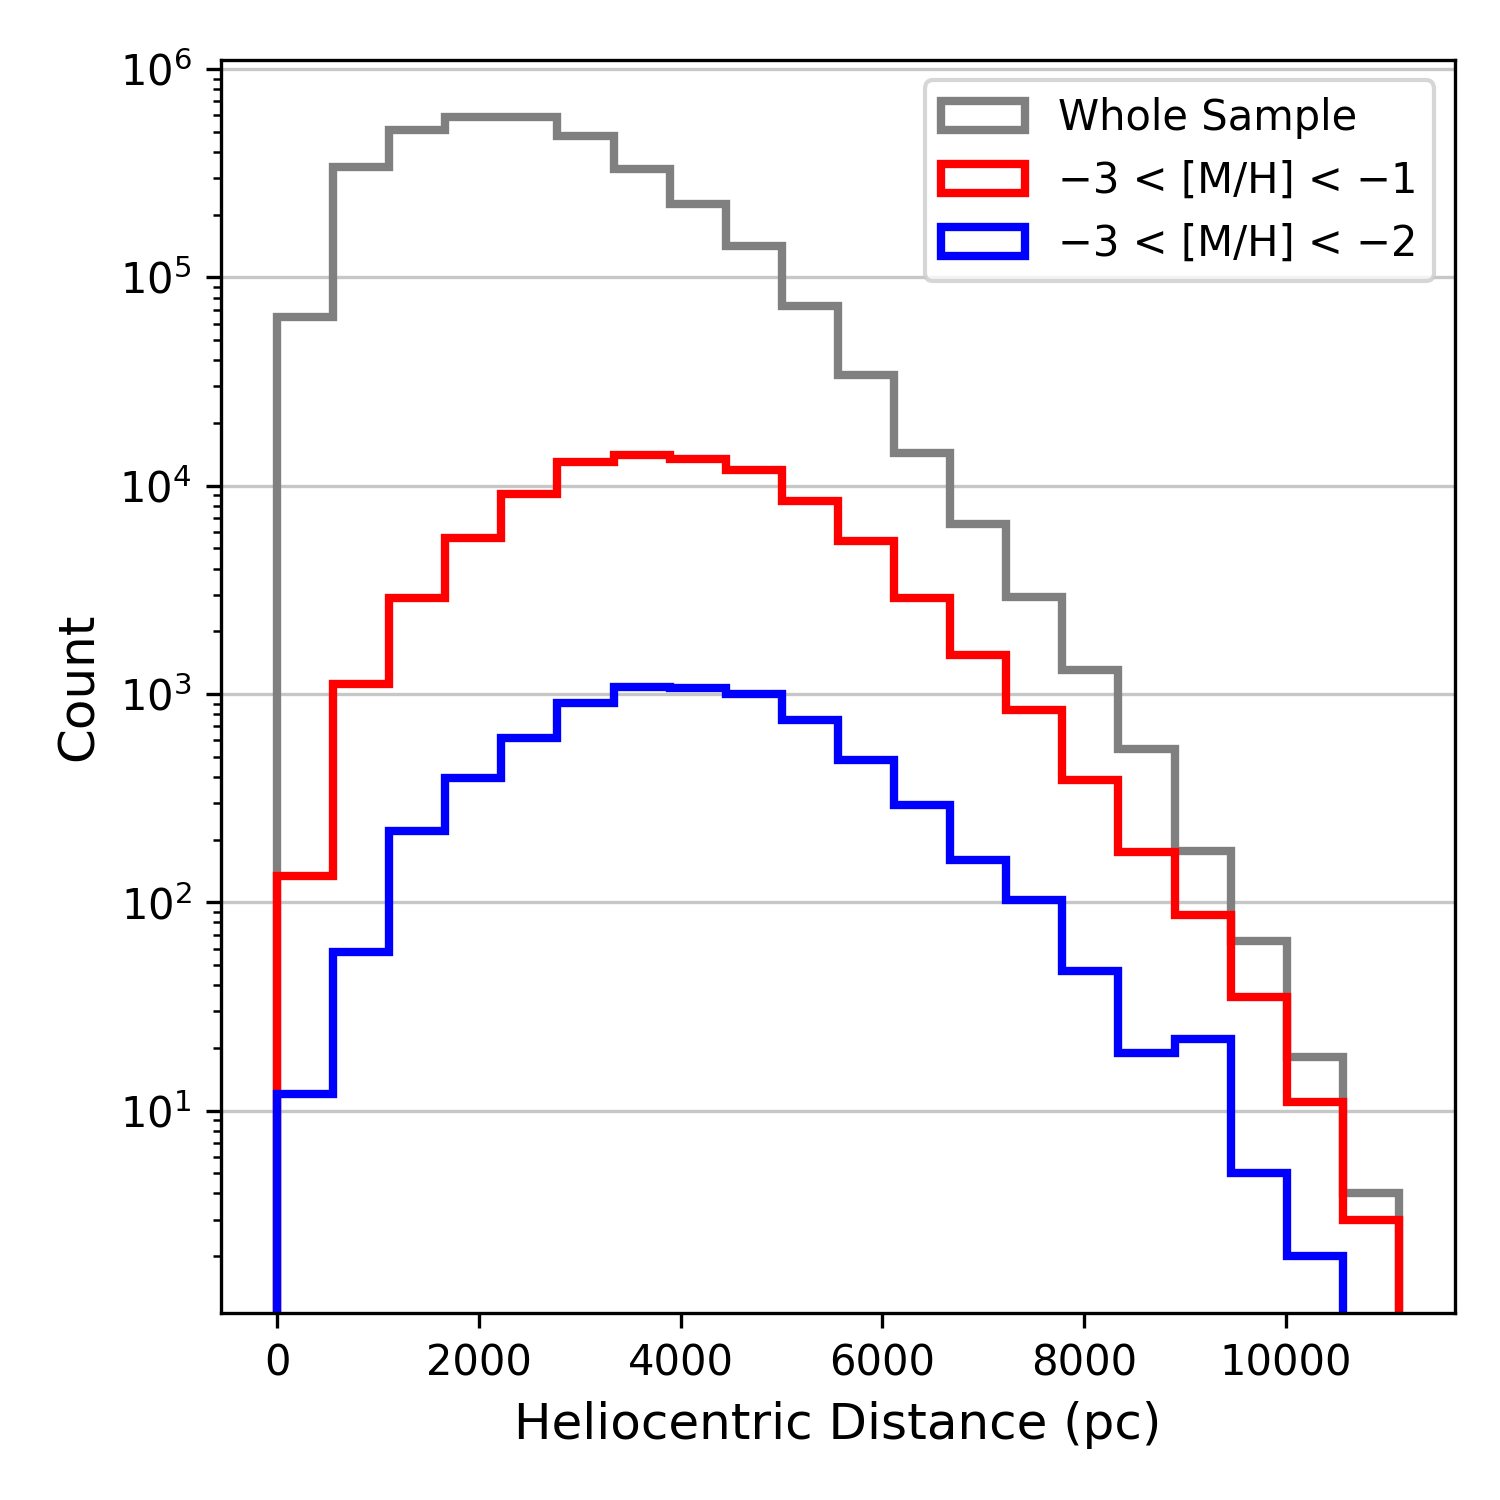
\includegraphics[width=\textwidth]{../figures/distance_histogram.png}
    \caption{Heliocentric distance}
    \label{fig:dist_hist}
  \end{subfigure}\hfill
  %--- Middle panel -----------------------------------------------------------
  \begin{subfigure}[b]{0.32\textwidth}
    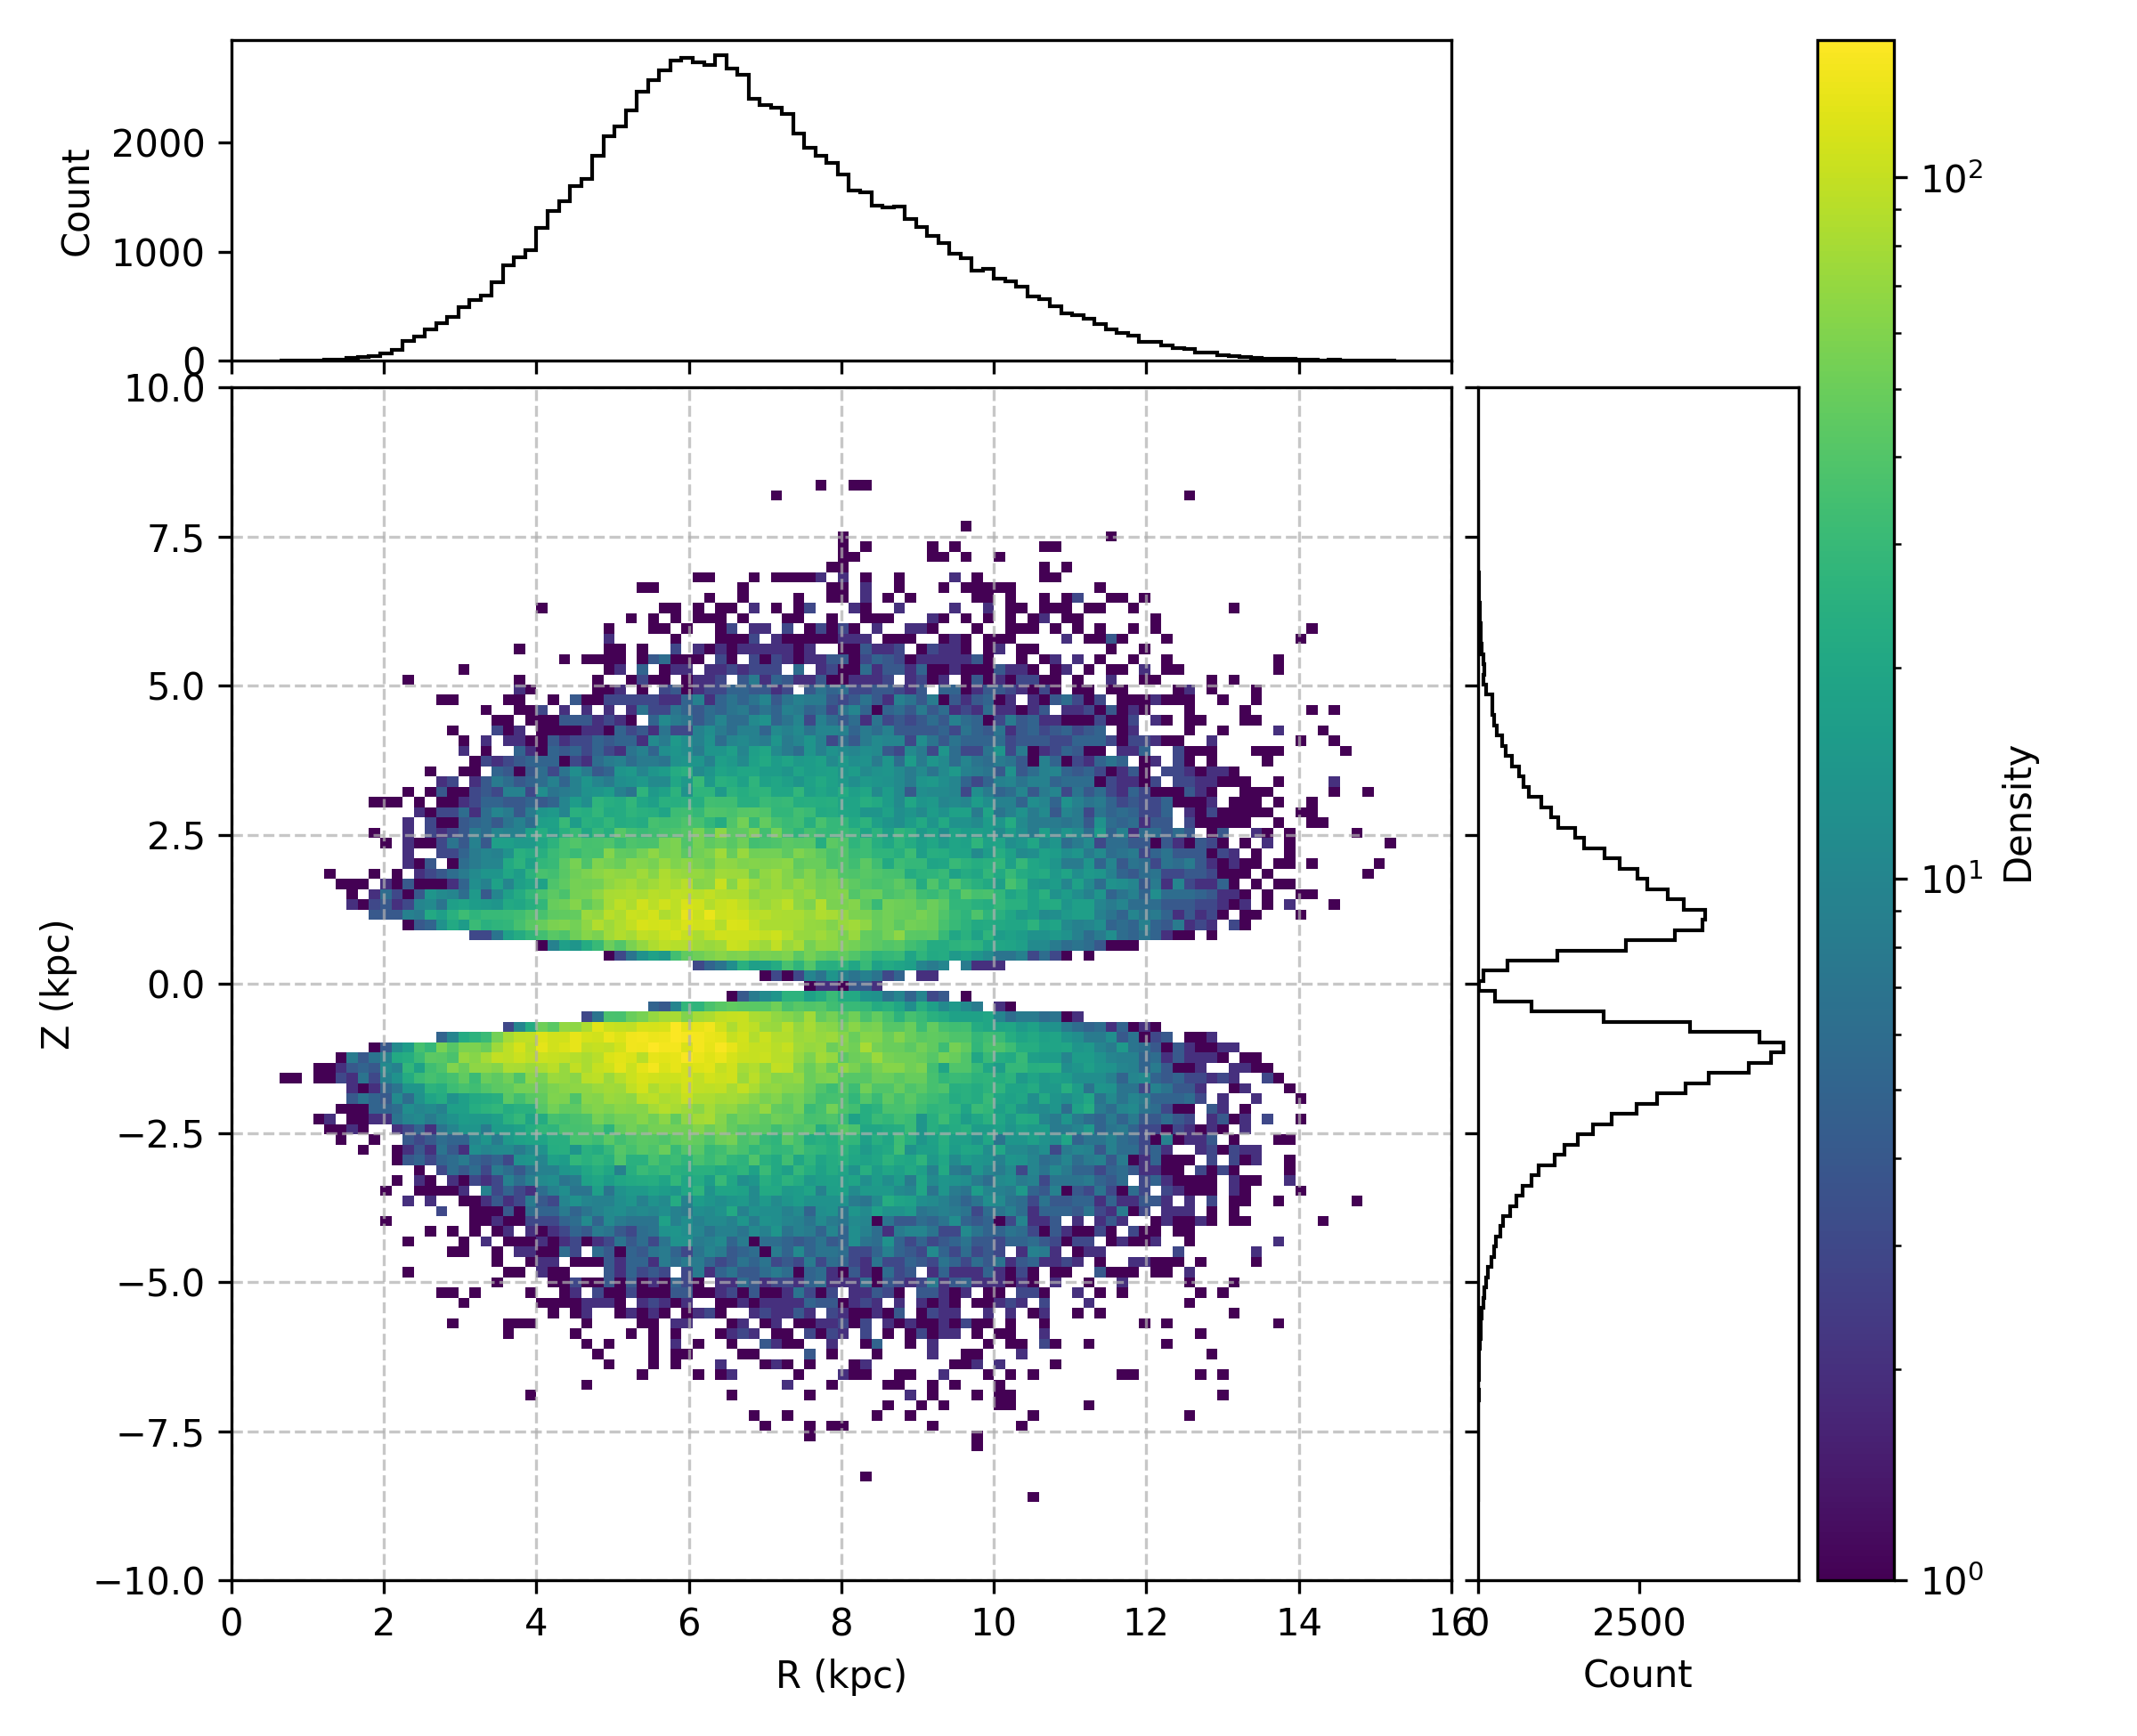
\includegraphics[width=\textwidth]{../figures/ZR_distribution.png}
    \caption{$R$–$Z$ distribution}
    \label{fig:ZR_dist}
  \end{subfigure}\hfill
  %--- Right panel ------------------------------------------------------------
  \begin{subfigure}[b]{0.32\textwidth}
    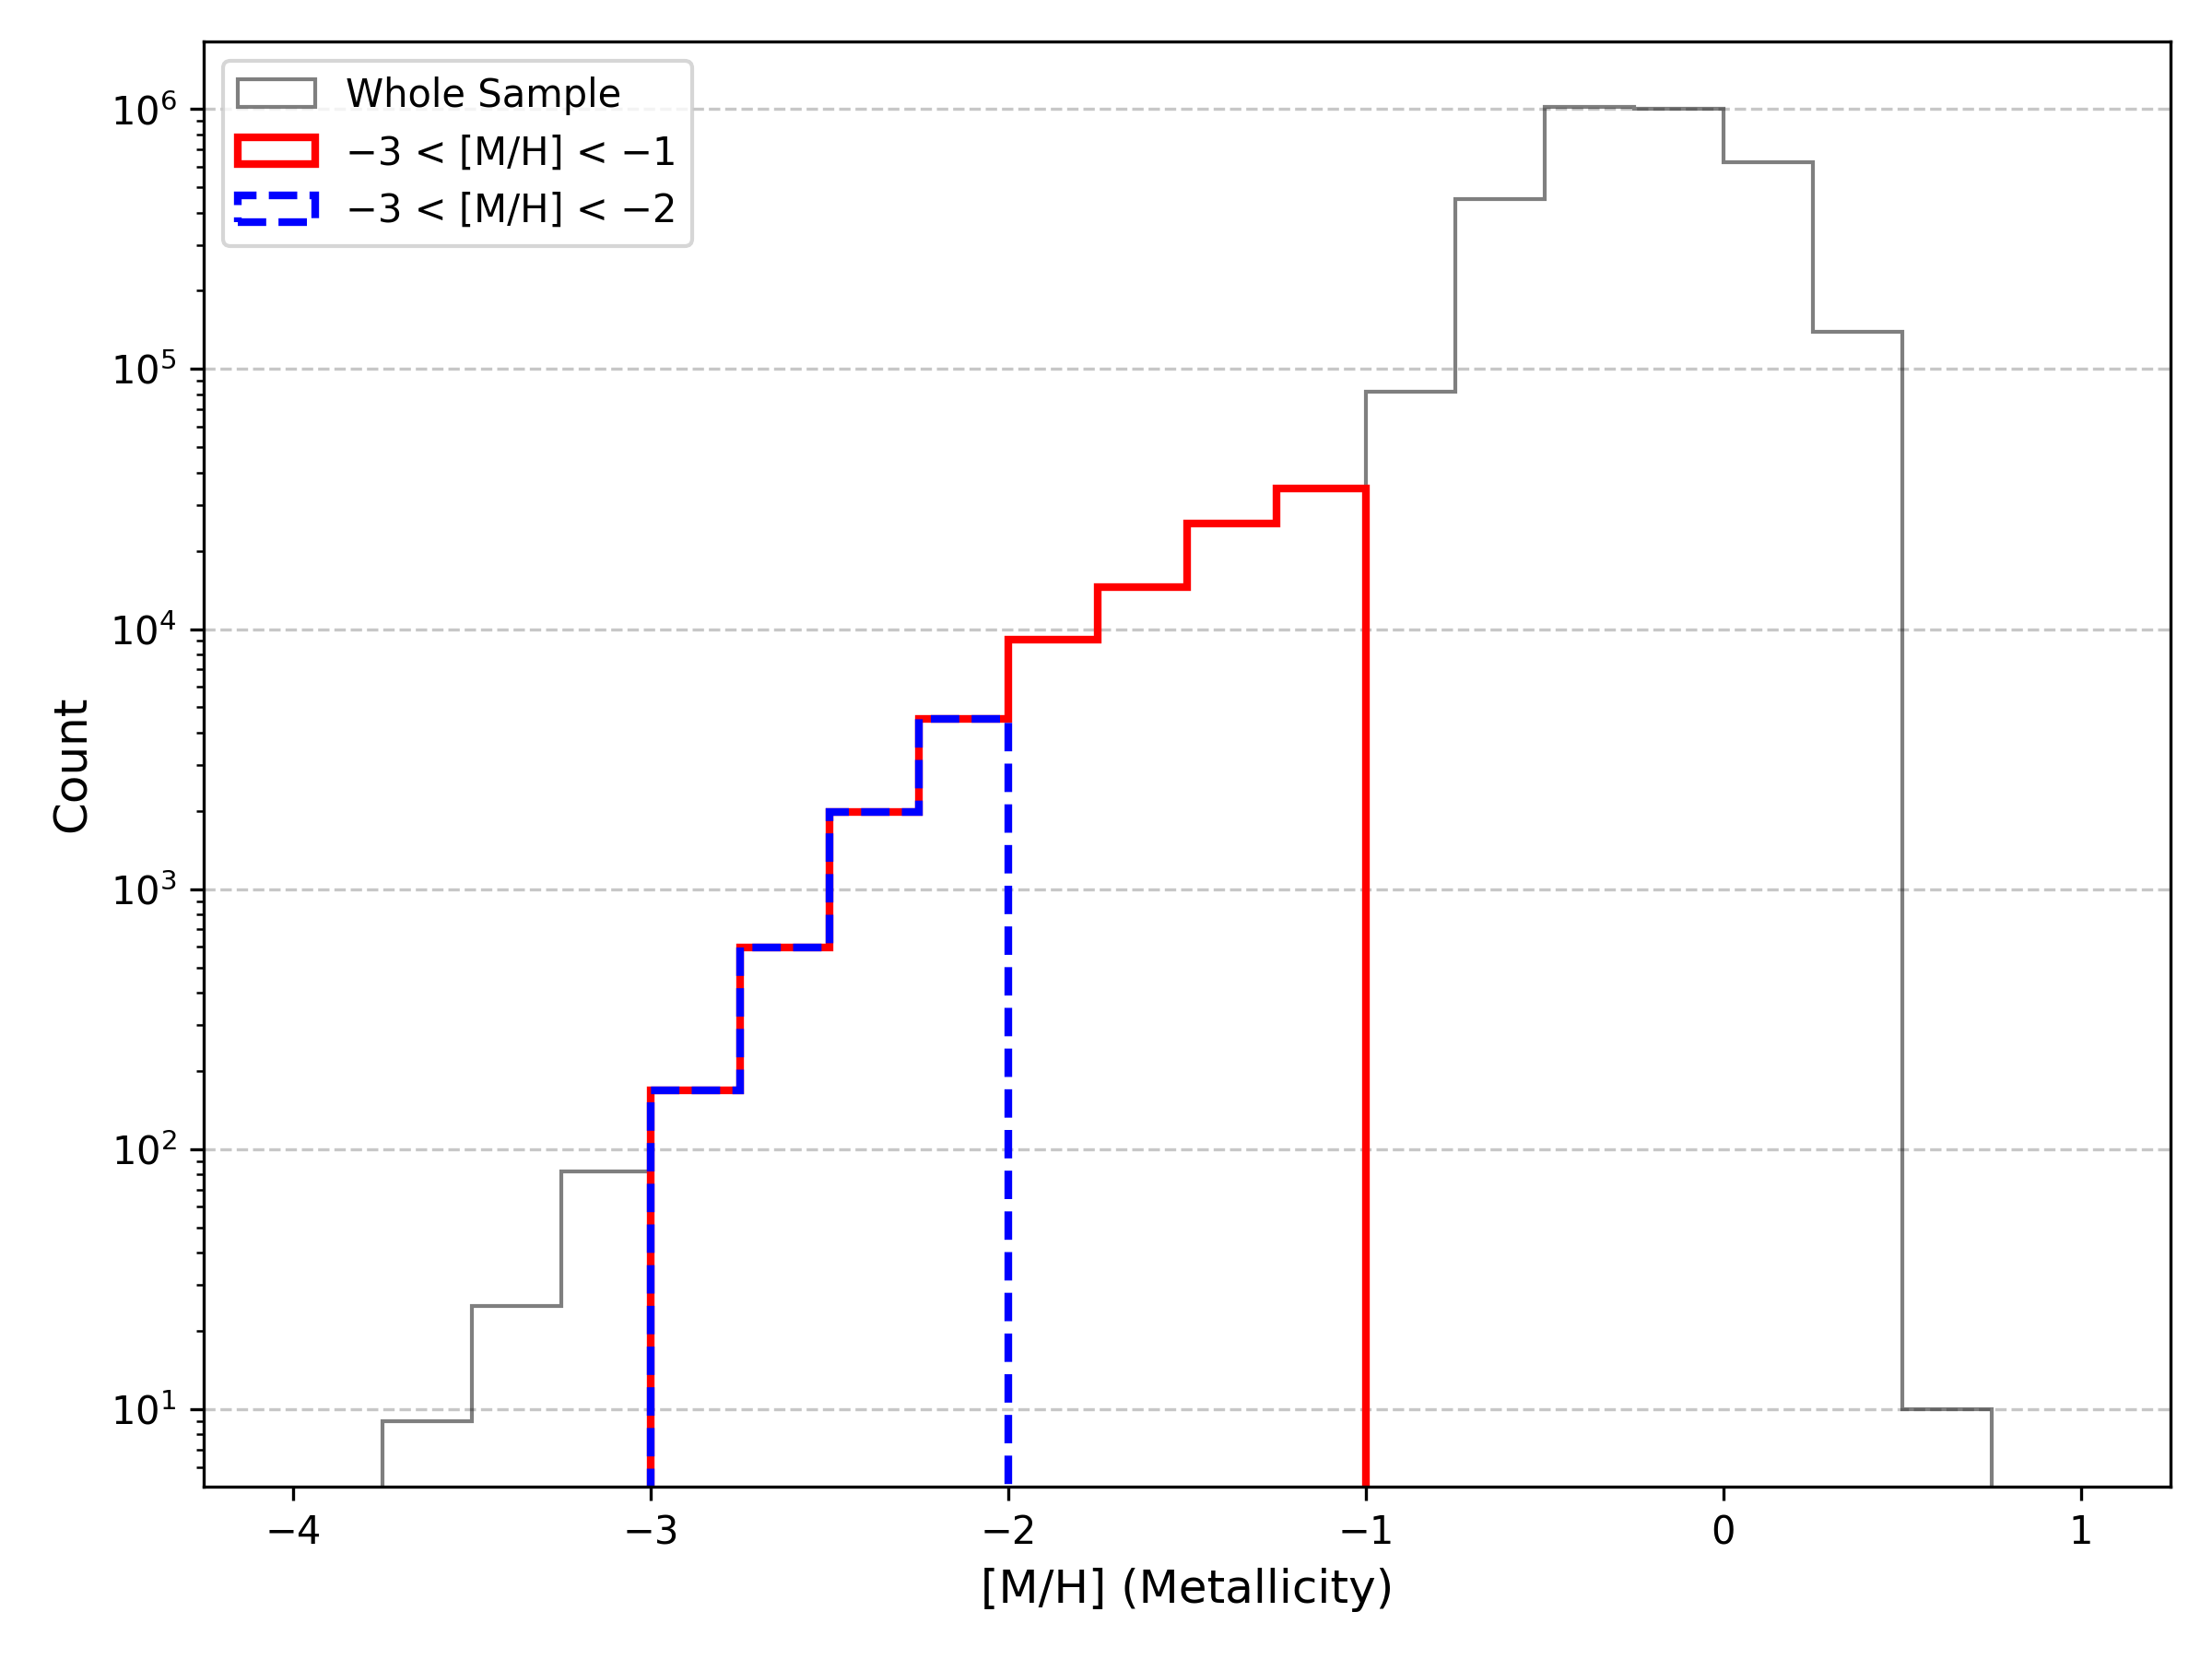
\includegraphics[width=\textwidth]{../figures/metallicity_distribution.png}
    \caption{Metallicity}
    \label{fig:met_dist}
  \end{subfigure}

  \caption{Properties of the final RGB sample after all quality and footprint cuts.
           \textit{Left:} heliocentric-distance histogram for the whole sample (grey); the
           subsets with $-3<\mathrm{[M/H]}<-1$ and $-3<\mathrm{[M/H]}<-2$ are shown in
           solid red and dashed blue, respectively.  
           \textit{Middle:} density map in Galactocentric cylindrical coordinates.  
           The empty band at low $|Z|$ is a selection artefact of our
           latitude/extinction cuts, which deliberately remove the thin–disc mid-plane;
           the concentration around $R\!\simeq\!5$–$8$\,kpc reflects the volume
           accessible to bright RGB stars interior to the Solar circle and coincides
           with the molecular ring region where the stellar surface density peaks.  
           \textit{Right:} Metallicity distribution of our data sample. Line colours are the same as in the left panel.}
  \label{fig:data_properties}
\end{figure}

\subsection{Galactocentric Positions and Velocities}
\label{subsec:velocities}

Six–dimensional phase–space coordinates are obtained with
astropy.coordinates.  We adopt a Galactocentric frame
with $R_{0}=8.1$\,kpc and $Z_{0}=25$\,pc \citep{McMillan2016}, and a solar
velocity\footnote{Cartesian components $(U,V,W)$, where $U$ is radially
outwards, $V$ is aligned with Galactic rotation, and $W$ points to the
North Galactic Pole.}
$(U_{\odot},V_{\odot},W_{\odot})=(11.1,\,245,\,7.25)$\,km\,s$^{-1}$
\citep{Schonrich2010}.
The cylindrical velocity components
$(v_{R},v_{\phi},v_{Z})$ are extracted from the transformed
SkyCoord module.

To propagate measurement errors we generate
$N_{\rm MC}=100$ Monte–Carlo realisations per star, drawing
parallax, proper motions, radial velocity, and distance from their
reported uncertainties (the proper–motion covariance is honoured
through a bivariate normal).  Each realisation is transformed to the
Galactocentric frame, yielding distributions of
$v_{R}$, $v_{\phi}$, and $v_{Z}$; the $1\sigma$ widths of those
distributions are stored as per–star velocity uncertainties.




\begin{figure}
  \centering
  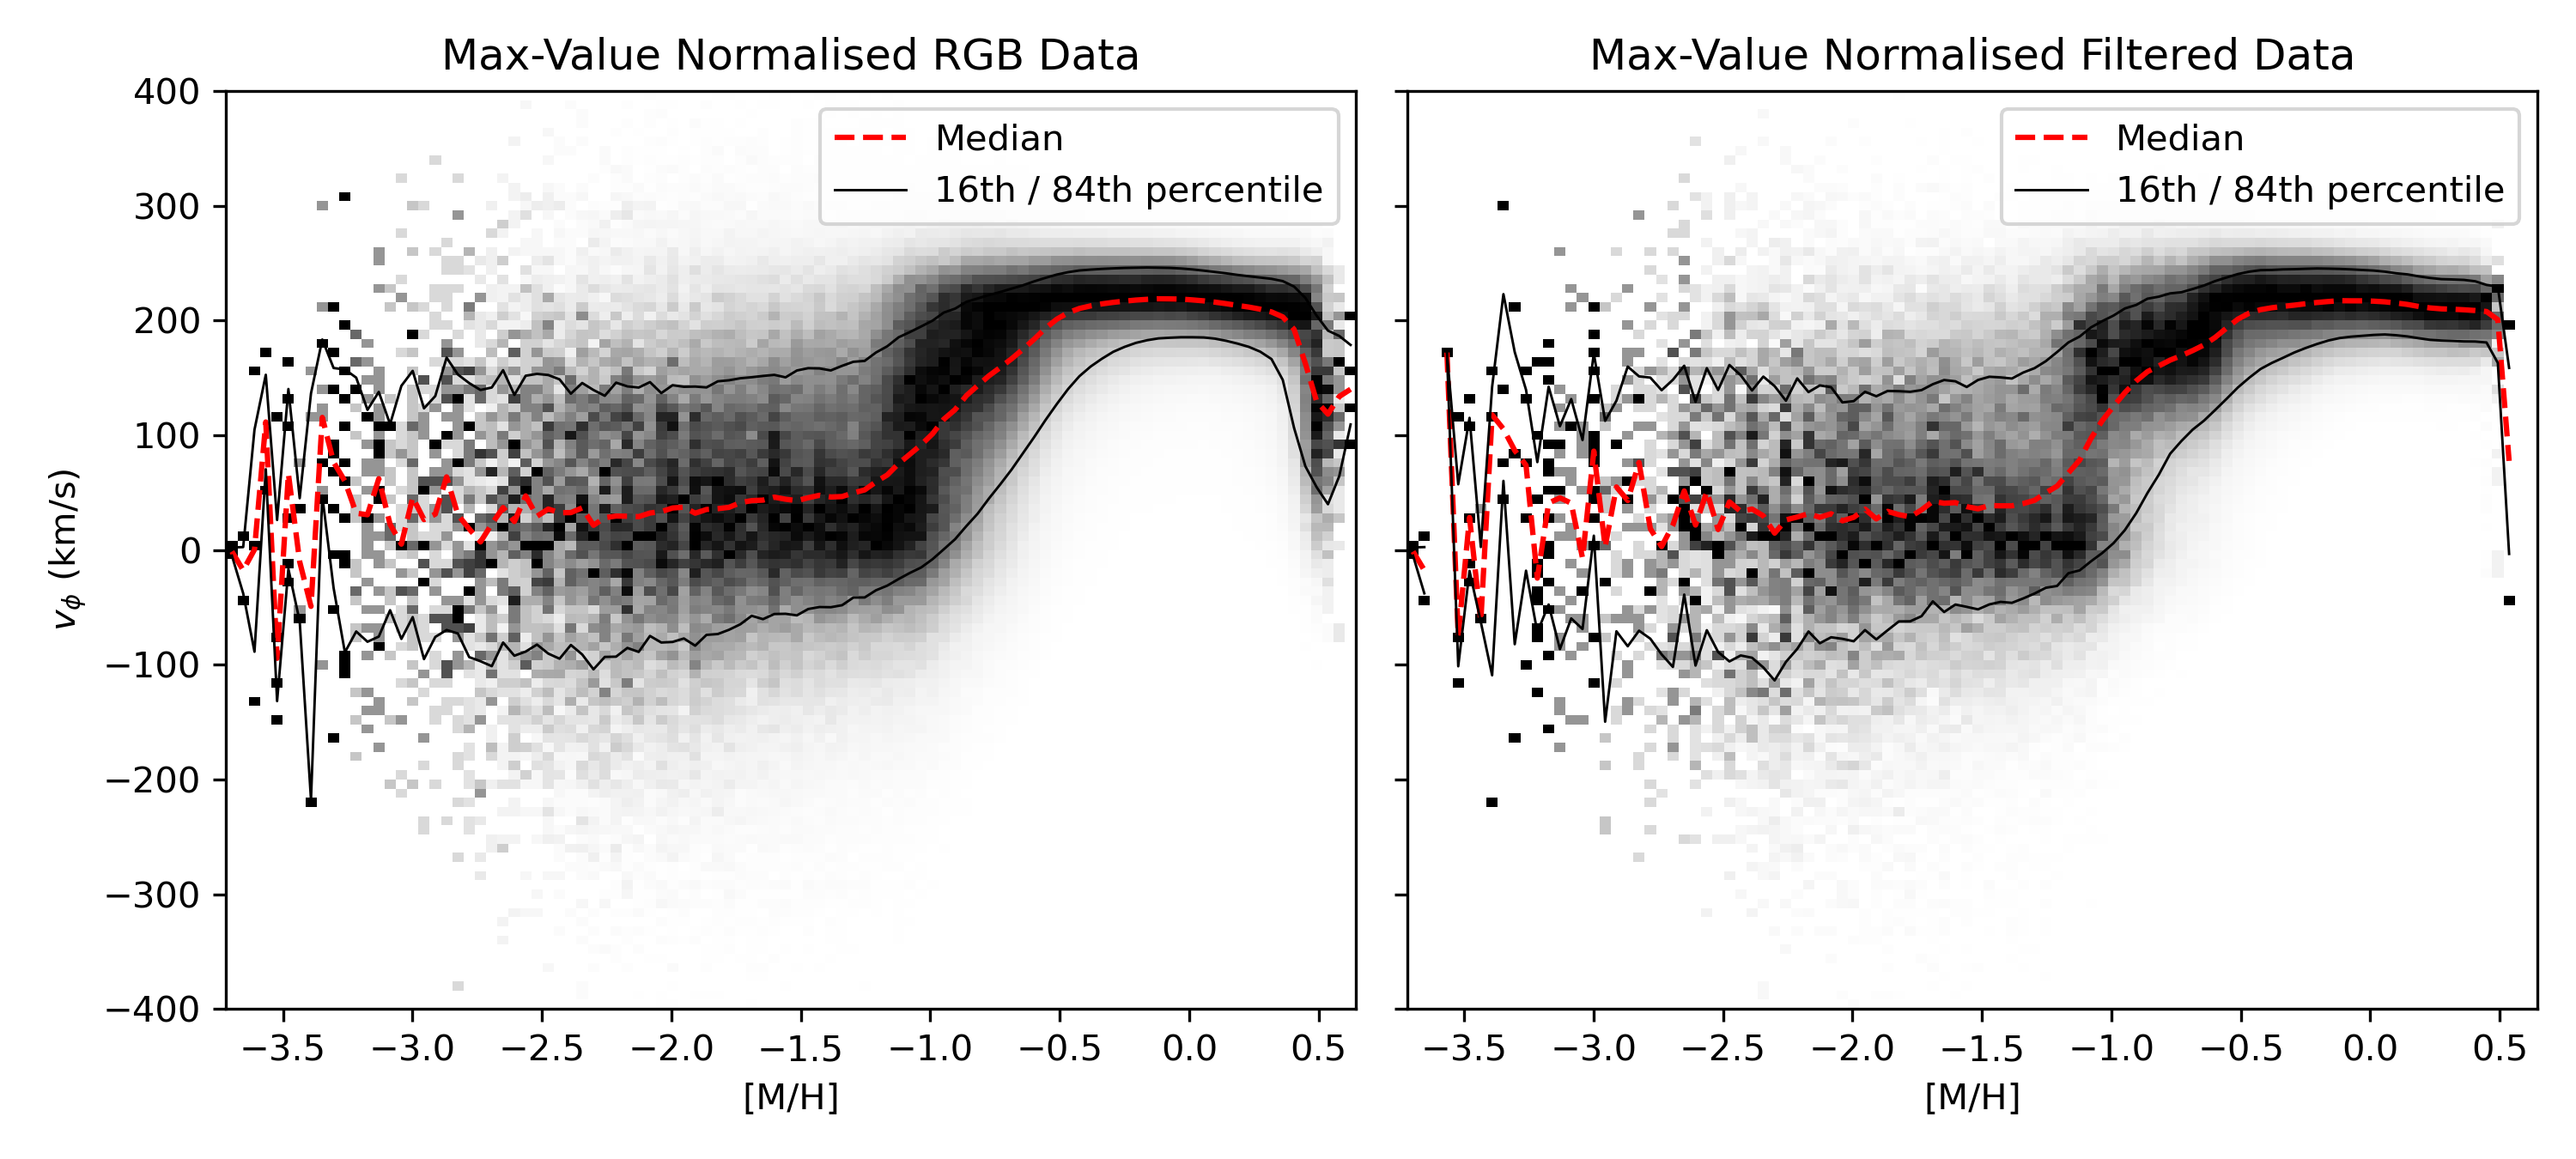
\includegraphics[width=0.94\textwidth]{../figures/vphi_histograms_with_tracks.png}
  \caption{Column-normalised density in the $v_{\phi}$–[M/H] plane.
           \textit{Left:} the bright-RGB catalogue of \citet{Andrae2023}.
           \textit{Right:} the same sample after all distance,
           dust, and quality cuts.  Greyscale pixels show the normalised
           counts in each metallicity bin; the red dashed curve is the
           median $v_{\phi}$, and the black curves trace the 16$^{\text{th}}$
           and 84$^{\text{th}}$ percentiles.}
  \label{fig:vphi_tracks}
\end{figure}



As shown in Figure~\ref{fig:vphi_tracks}, stellar azimuthal velocities
evolve increase with metallicity.  Halo–like kinematics dominate at
${\rm [M/H]}\lesssim-1.5$ with statstics
indicative of a pressure-supported component.  A rapid spin-up appears over the 
metallicity range ${\rm [M/H]} \simeq -1.3$ to $-0.9$, consistent with \citet{Belokurov2022}.
By ${\rm [M/H]}\gtrsim-0.5$ the stellar azimuthal velocities reaches the Local
Standard-of-Rest value ($\approx220\;\mathrm{km\;s^{-1}}$) and the
velocity dispersion dispersion falls, marking the
transition to a disc.  Visually, using \ref{fig:vphi_tracks}, we can observe
that the onset of ordered rotation in the Milky Way occurred when the inter-stellar medium
reached roughly one-tenth solar metallicity.


\begin{figure}
  \centering
  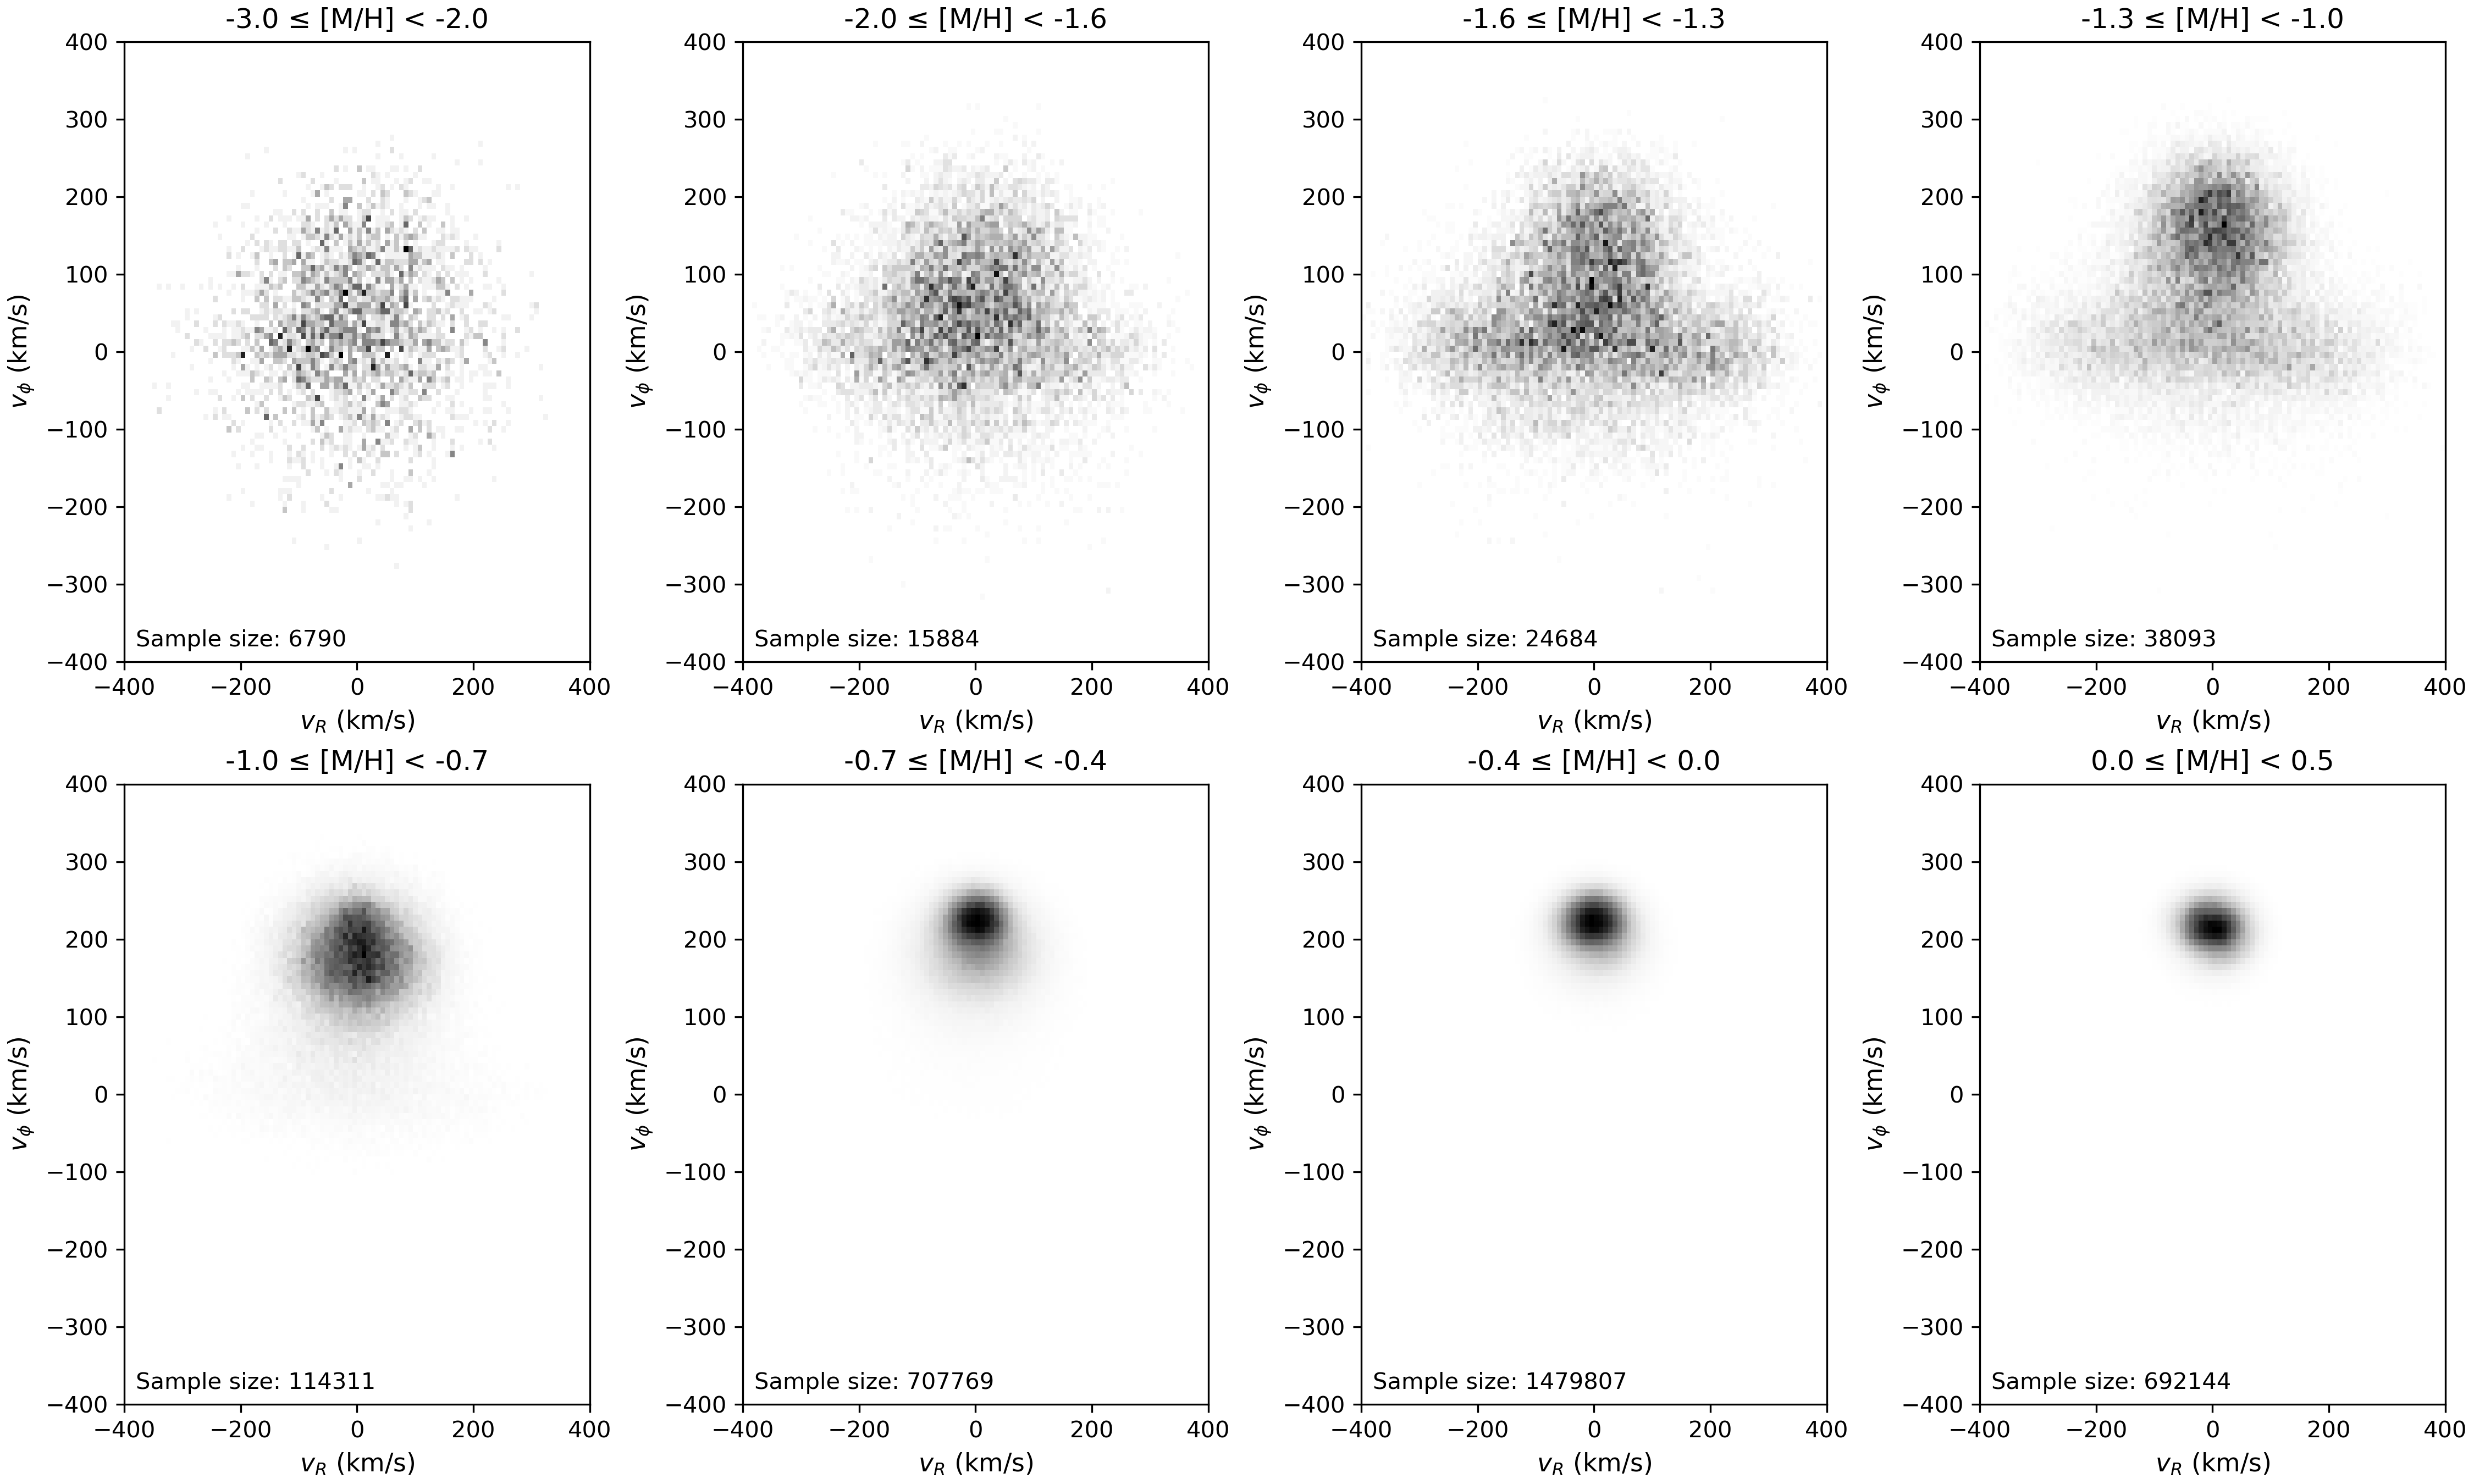
\includegraphics[width=\textwidth]
                   {../figures/vphi_metallicity_histograms.png}
  \caption{Galactocentric velocity distributions as a function of metallicity.
           Each panel shows the column–normalised density of stars in the
           $v_R$–$v_\phi$ plane for the metallicity interval printed at the
           top. With increasing metallicity the distribution contracts in both
           directions—signalling lower velocity dispersion—while the bulk
           of stars moves upward to larger prograde azimuthal velocity.
           }
  \label{fig:vRvphi_bins}
\end{figure}


\begin{figure}
  \centering
  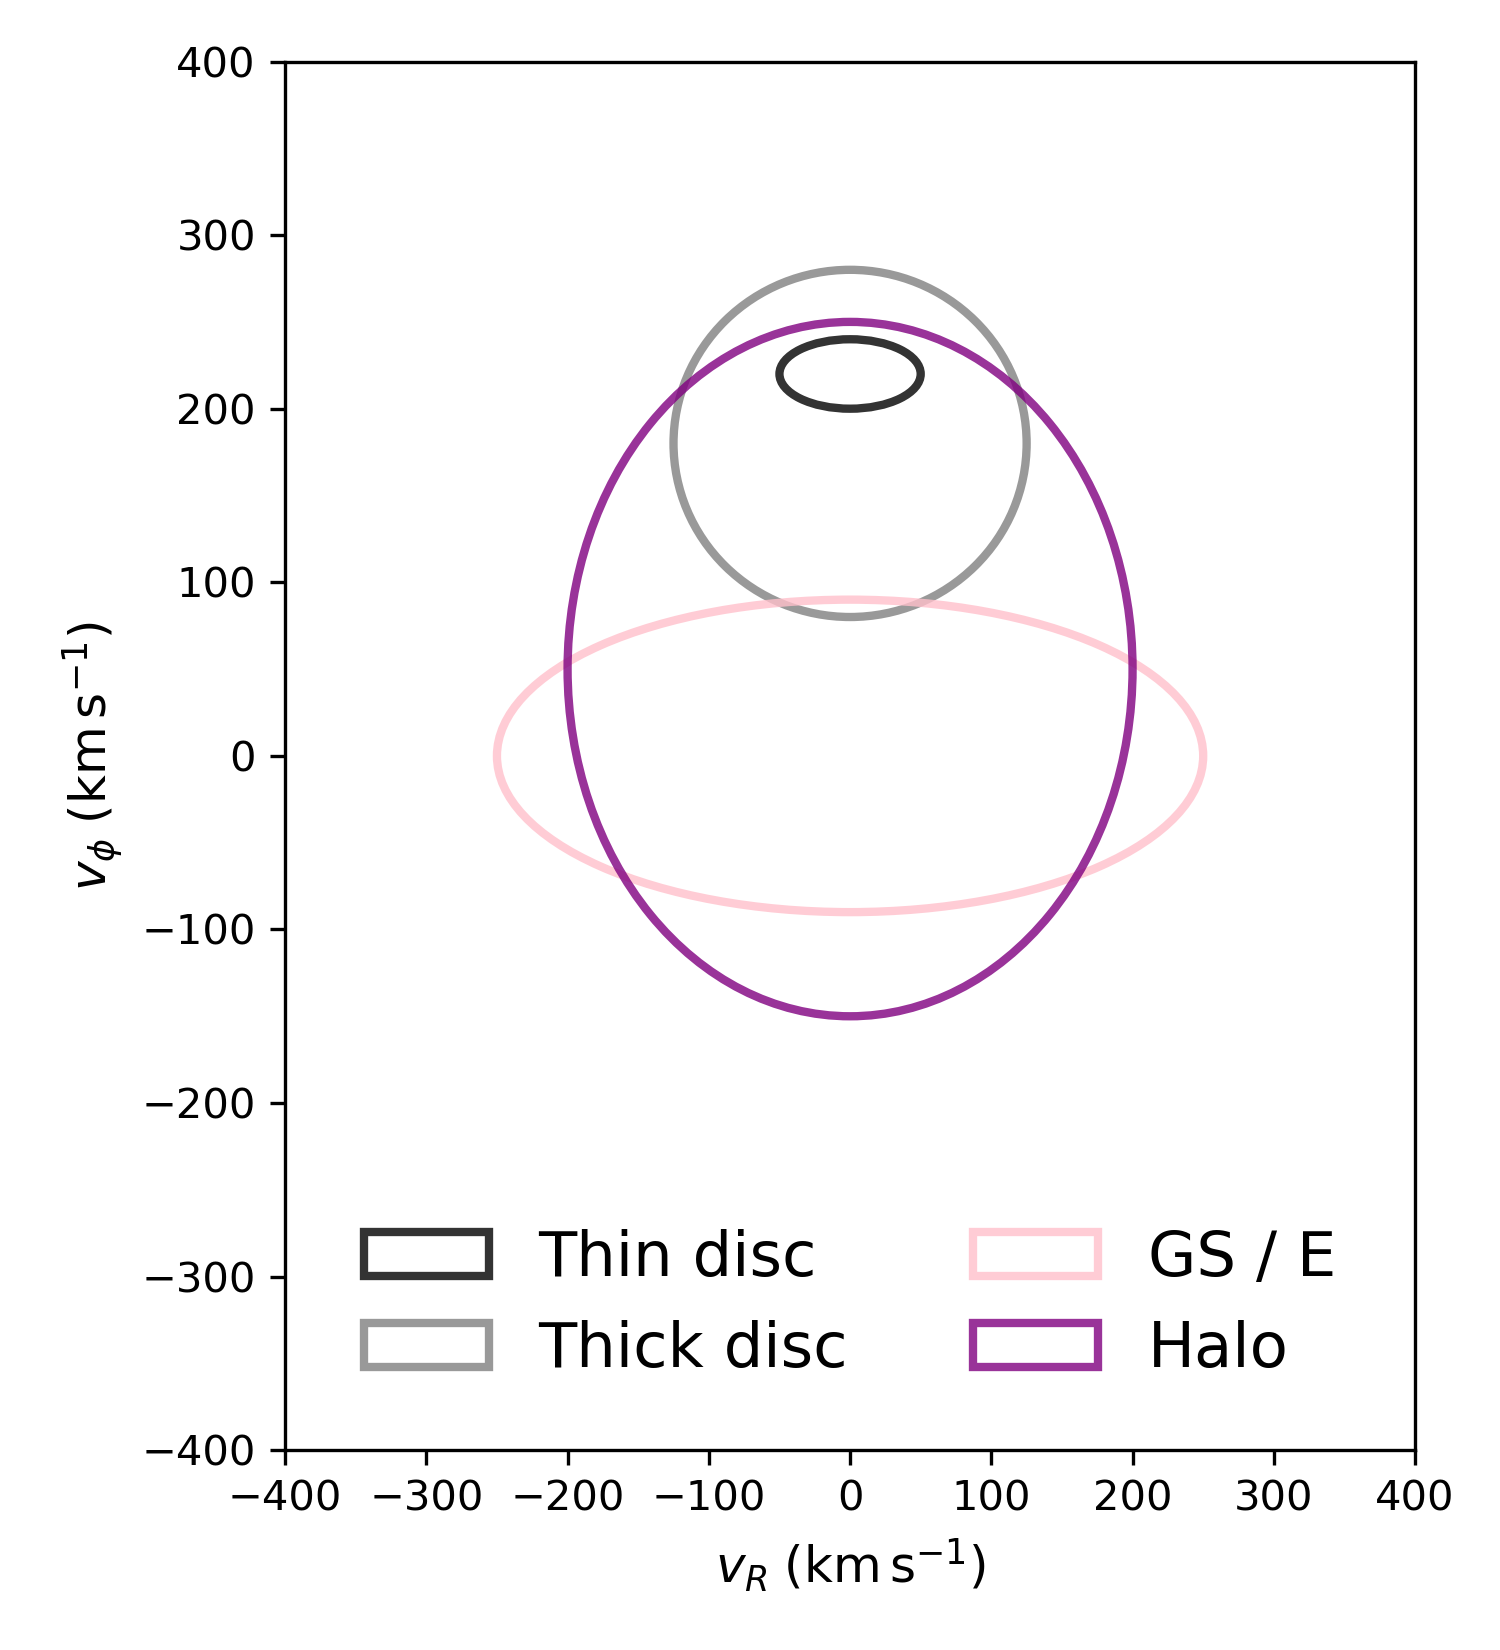
\includegraphics[width=0.3\columnwidth]
                   {../figures/reference_velocity_ellipses.png}
  \caption{Ellipses mark the approximate extent of the thin disc
           (\textcolor{black}{black}), thick disc (\textcolor{gray}{grey}),
           Gaia–Sausage/Enceladus debris (\textcolor{pink}{pink}) and the
           pressure-supported stellar halo (\textcolor{purple}{purple}).
           The figure serves as a visual key for interpreting the data panels
           in Fig.~\ref{fig:vRvphi_bins}.}
  \label{fig:ref_ellipses}
\end{figure}

As shown in Fig.~\ref{fig:vRvphi_bins}, stars with
${\rm[M/H]}\!\geq\!-1.0$ have a strong prograde bias in azimuthal velocities, 
with a peak at $v_\phi\!\gtrsim\!180$ km s$^{-1}$ and a relatively narrow
distribution in $v_R$. As shown in Fig.~\ref{fig:ref_ellipses}, this is consistent with 
the thin– and thick-disc ellipses. 
Below ${\rm[M/H]}\simeq-1.0$ the distribution broadens and
drops toward $v_\phi\!\approx\!0$, indicating
pressure supported kinematics, characteristic of the stellar halo and
the radial Gaia–Sausage/Enceladus debris.  At the lowest
metallicities (${\rm[M/H]}\lesssim-1.5$) the contours are nearly
isotropic with only a mild prograde bias.  Hence, any
rotation-supported very-metal-poor disc must contribute at most a
small fraction of the population. In subsequent analysis we quantitatively assess
these observations.

Given we are testing whether a very-metal-poor stellar disc exists, we naturally 
restrict the sample to stars within \mbox{$|Z|<2.5$ kpc} of the galactic mid-plane. 
This keeps the focus on stars close to the plane, where any disc-like population 
(whether formed in situ or deposited by mergers) would be found \citep{Tkachenko_2025}.

Upon comparison with \citet{zhang2024existencemetalpoordiscmilky}, we note that our 
sample is approximately the same size - with a difference of less than 0.002\% of the sample size in each bin.



\section{Methodology}

\subsection{Gaussian Mixture Model}

To quantitatively investigate the kinematic structure of metal-poor stars and assess 
the presence of a potential very-metal-poor disc, we use a Gaussian Mixture Model (GMM) framework
 as done by \citet{zhang2024existencemetalpoordiscmilky}. 
GMMs are a class of unsupervised machine learning algorithms commonly used in data science 
for clustering and density estimation. They model a dataset as a weighted sum of multivariate 
Gaussian distributions, each corresponding to a latent sub-population within the data.

From a probabilistic perspective, the GMM assumes that each observed data point is generated from a 
hidden (latent) variable indicating membership in one of the Gaussian components. This latent space 
formulation allows the model to assign probabilistic classifications to data points, providing a 
soft clustering where each star has a fractional likelihood of belonging to each component. In our case, 
the data are three-dimensional velocity vectors $(v_R, v_\phi, v_Z)$, and the latent space captures 
distinct kinematic substructures in this space.

We implement the GMM fitting using the pyGMMis package \citep{pygmmis} in the $v_R$, $v_\phi$, and $v_Z$
phase space. This algorithm extends the standard 
Expectation-Maximisation (EM) algorithm with the ``Extreme Deconvolution'' technique developed by 
\citet{Bovy2011}. This method is particularly well-suited to astronomical datasets, as it incorporates 
measurement uncertainties into the GMM fitting by modifying the EM updates to account for known errors 
on each data point. In our case, these uncertainties are derived from the Gaia astrometric and 
spectroscopic data and are represented by diagonal covariance matrices encoding the squared uncertainties 
in $v_R$, $v_\phi$, and $v_Z$ for each star.


\subsection{Number of Gaussian Components}
\label{subsec:n_components}

We apply the GMM separately to each metallicity bin with ${\rm [M/H]} < -1$, as we are specifically 
interested in detecting any rotationally supported structure among the very metal-poor stars. An important decision 
must be made when implementing the appropriate number of components in applying Gaussian Mixture Models. Too few 
components may underfit the data, missing real substructures, while too many will overfit, leading to spurious 
and physically uninterpretable results.

We select the optimal number of components using the Bayesian Information Criterion (BIC) \citealt{Schwarz1978}. 
The BIC is defined as

\begin{equation}
\mathrm{BIC} = k \ln(n) - 2 \ln \mathcal{L},
\end{equation}

where $k = (1 + 3 + 6) \times N - 1$ is the total number of free parameters in a model with $N$ Gaussian components 
(accounting for the weights, means, and covariances), $n$ is the number of stars in the sample, and $\mathcal{L}$ 
is the maximum likelihood of the fit. The BIC penalizes model complexity, such that adding extra components 
without a significant gain in likelihood will result in a higher BIC value.

\begin{figure*}[h]
    \centering
    \begin{subfigure}[t]{0.23\textwidth}
        \centering
        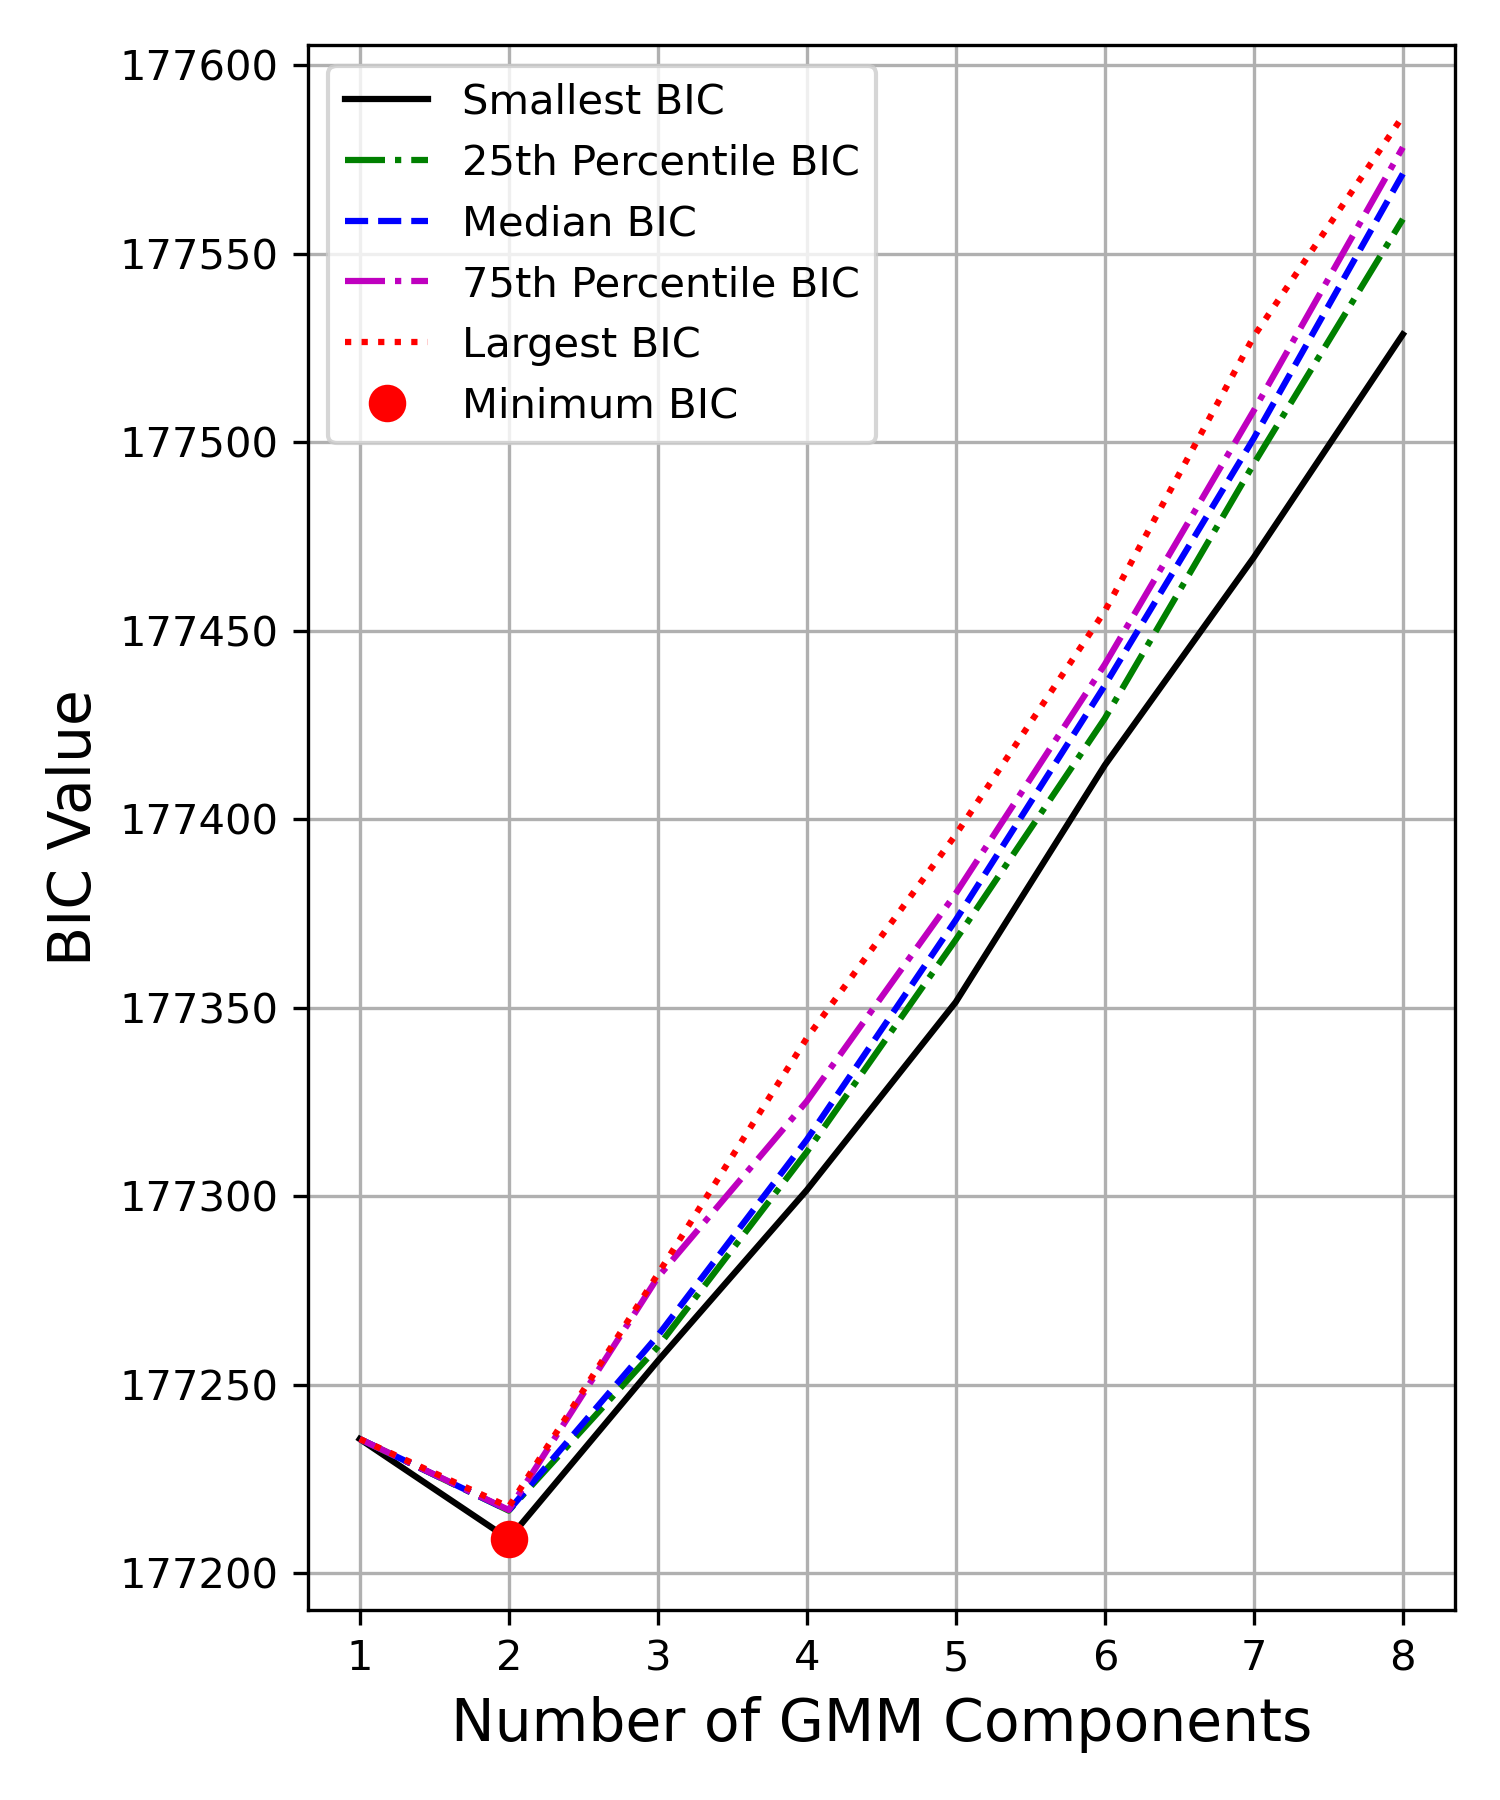
\includegraphics[width=\linewidth]{../figures/bic_vmp.png}
        \caption{$-3.0 < \mathrm{[M/H]} < -2.0$}
    \end{subfigure}
    \hfill
    \begin{subfigure}[t]{0.23\textwidth}
        \centering
        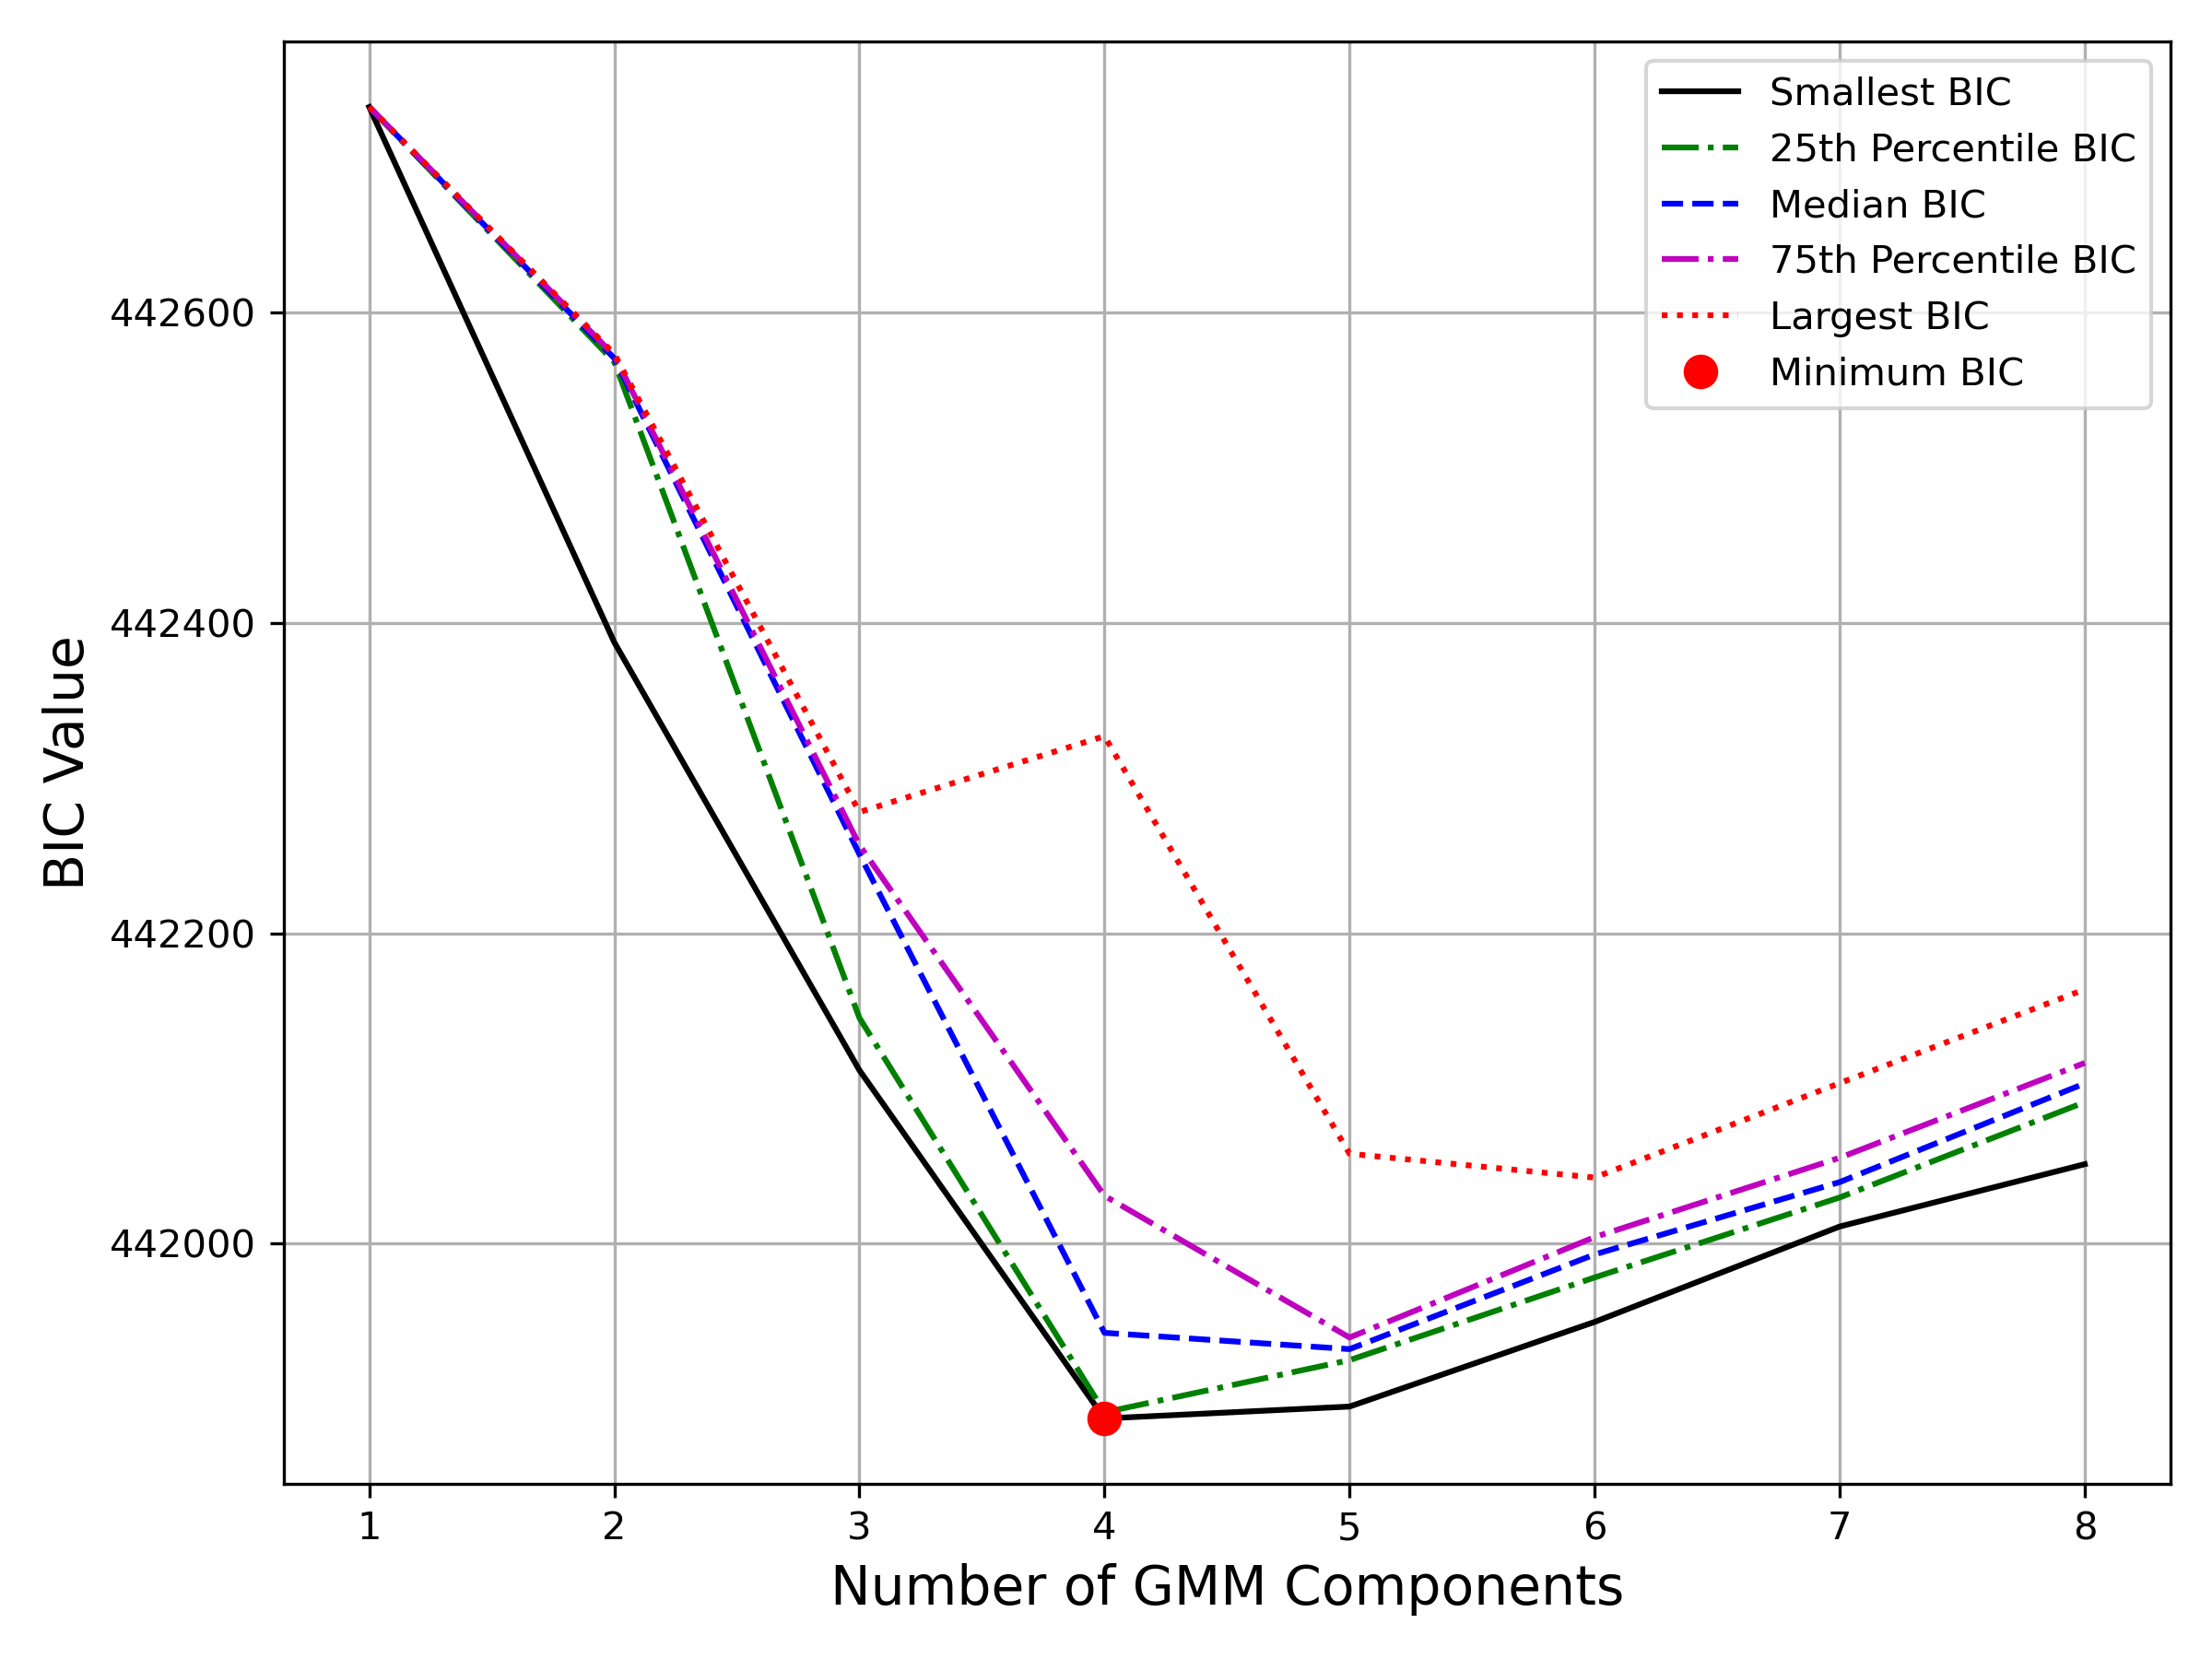
\includegraphics[width=\linewidth]{../figures/bic_imp.png}
        \caption{$-2.0 < \mathrm{[M/H]} < -1.6$}
    \end{subfigure}
    \hfill
    \begin{subfigure}[t]{0.23\textwidth}
        \centering
        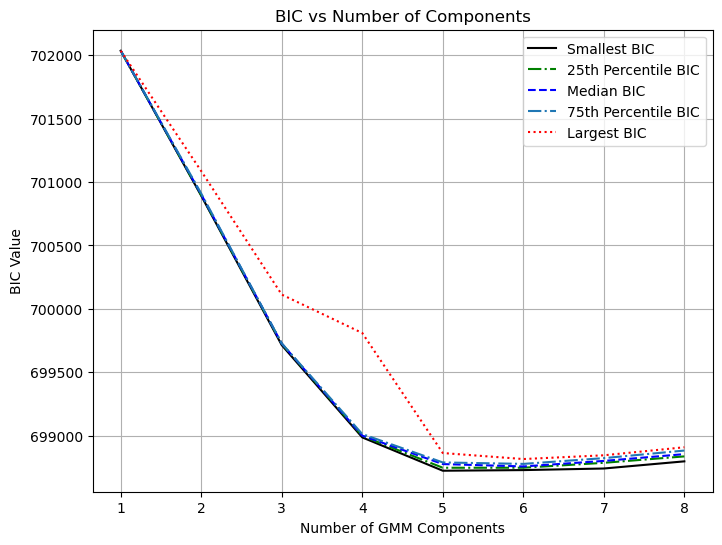
\includegraphics[width=\linewidth]{../figures/bic_mp1.png}
        \caption{$-1.6 < \mathrm{[M/H]} < -1.3$}
    \end{subfigure}
    \hfill
    \begin{subfigure}[t]{0.23\textwidth}
        \centering
        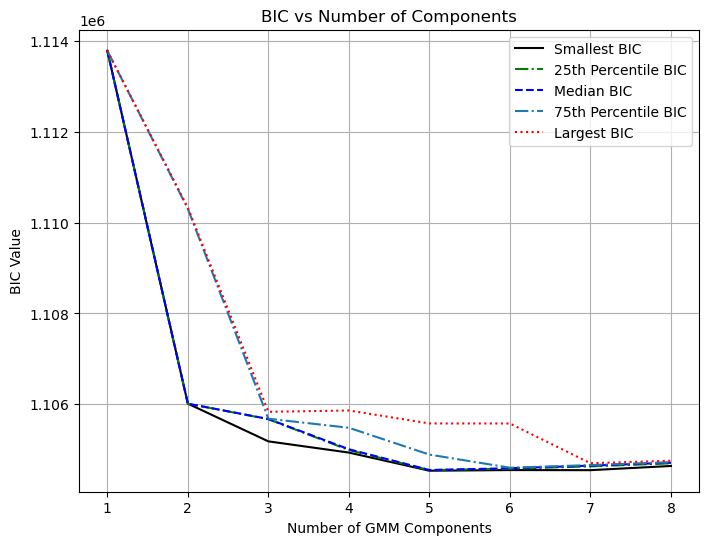
\includegraphics[width=\linewidth]{../figures/bic_mp2.png}
        \caption{$-1.3 < \mathrm{[M/H]} < -1.0$}
    \end{subfigure}

    \caption{BIC distributions as a function of the number of GMM components in each metallicity bin. The optimum number of components is indicated by the minimum BIC value (highlighted in red).}
    \label{fig:bic_vs_n_components}
\end{figure*}


The Expectation-Maximisation algorithm can become trapped in local minima, so we performed 50 initialisations 
for each $N$ and recorded the BIC value for each trial. The minimum BIC value across all trials indicated 
the statistically preferred model and suggests that the global optimum was likely reached. 

To improve convergence and model stability, the GMM components in each trial were initialised using the kmeans algorithm. 
This is is due to the sensitivity of GMMs to their starting conditions: poor initialisation can lead to convergence 
on undesirable solutions, particularly in high-dimensional or overlapping data. KMeans clustering provides an
initialisation point by partitioning the velocity space into compact, roughly spherical clusters. This works well with the 
assumptions of Gaussian components and often gives faster, more stable convergence and more physically meaningful results. 
In our application, where stellar substructures are partially overlapping in velocity space, this method applies well.

In Figure~\ref{fig:bic_vs_n_components}, we show the distribution of BIC values across four metallicity bins as
a function of $N$. The resulting preferred number of components are 2, 4, 5, and 5 for the VMP, IMP, MP1, and MP2 bins.
This is in agreement with the findings of \citet{zhang2024existencemetalpoordiscmilky}.
Our analysis, however, selects the lowest BIC each time, removing the need for a subjective choice of the number of components
when BIC values are very similar. \citet{zhang2024existencemetalpoordiscmilky}, when observing the BIC values for the MP1 bin 
chooses to use 5 components instead of 6 despite the BIC score for the 6-component model being lower than the 5-component model.

 
\section{Results}

\subsection{Gaussian Mixture Model Fit}
\label{subsec:gmm}

Using the number of components selected by the BIC criteria, we fit the GMM to the data in each metallicity bin as shown in 
Figure~\ref{fig:gmm_decompositions}. We increased the number of initialisations to 100 for the final fitting to ensure convergence to a
stable solution.

\begin{figure*}[h]
    \centering
    \begin{subfigure}[t]{0.24\textwidth}
        \centering
        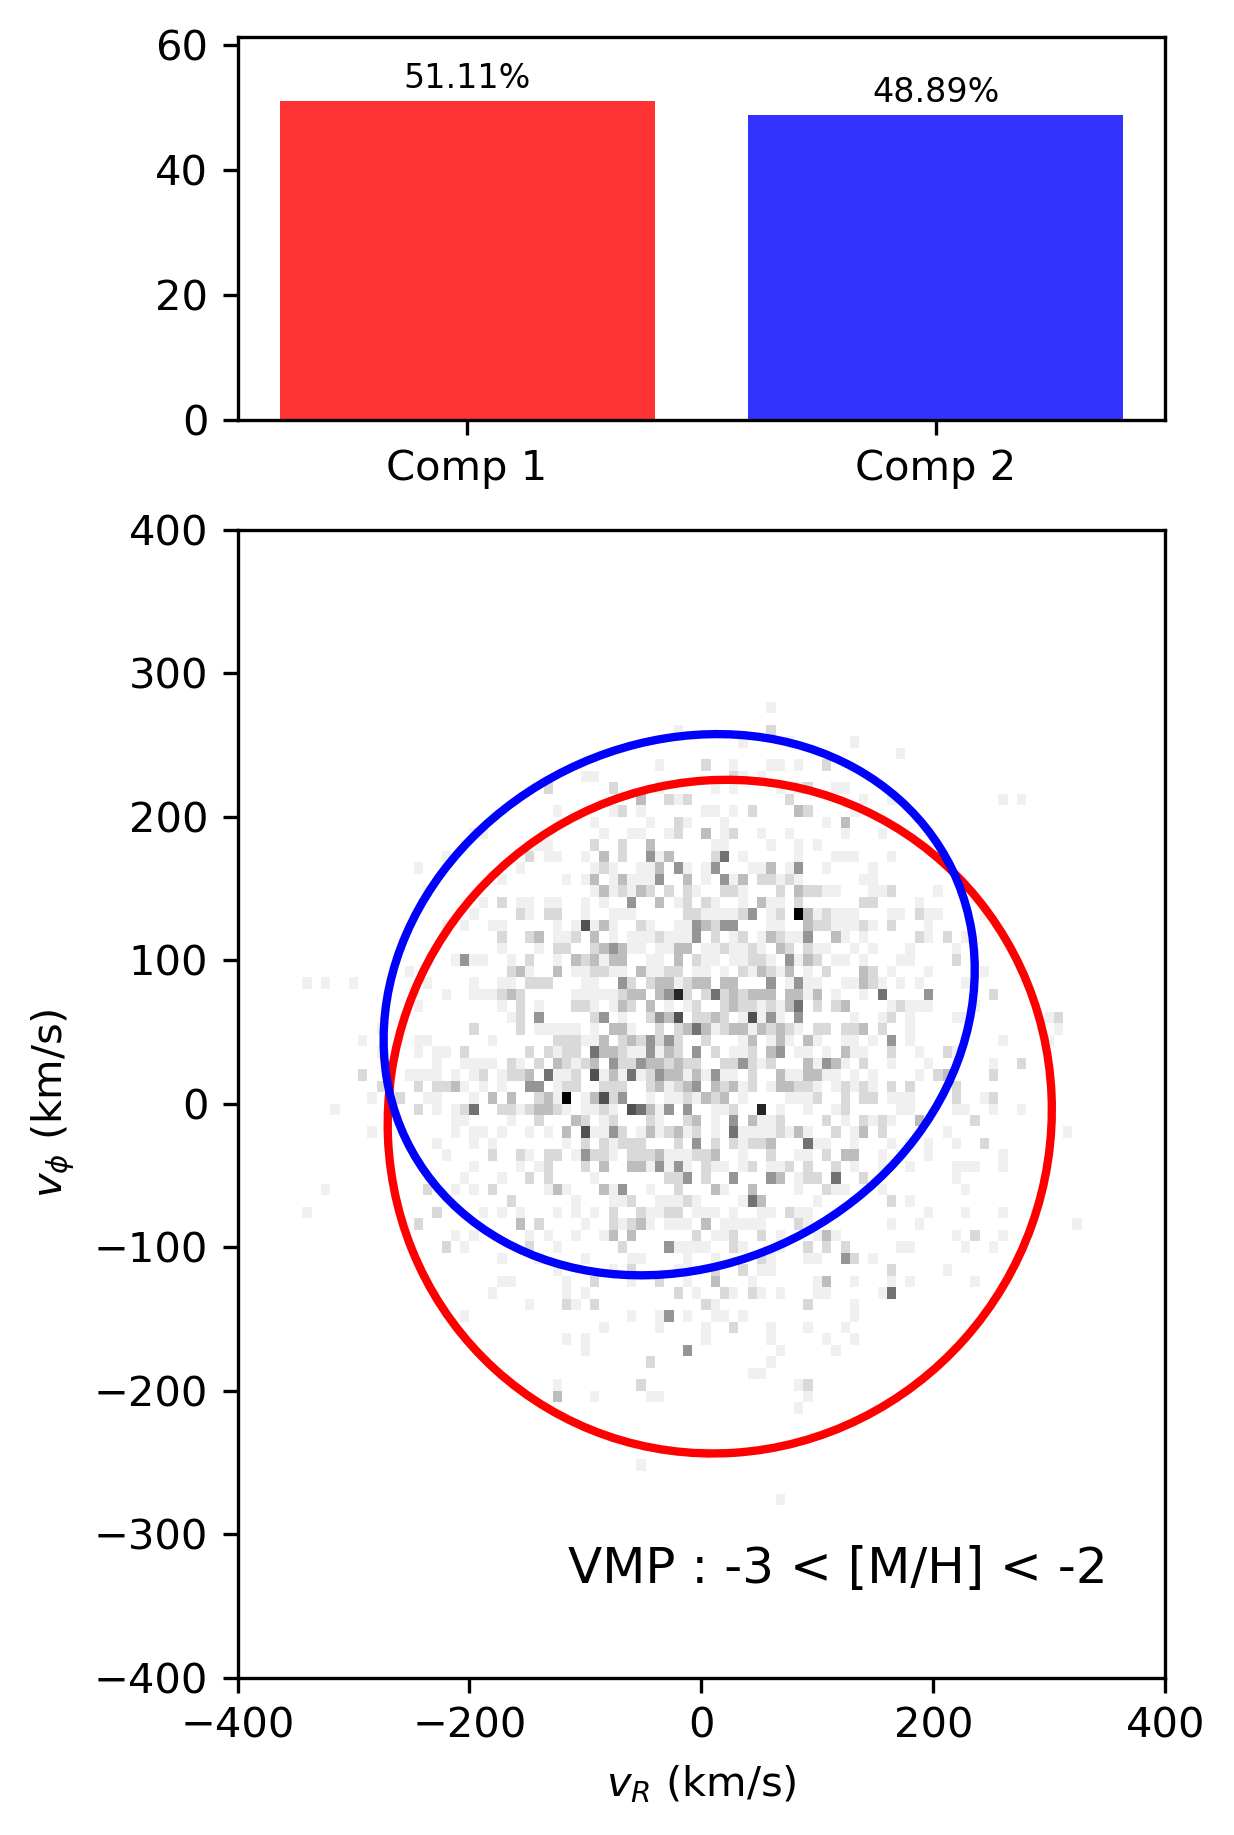
\includegraphics[width=\linewidth]{../figures/gmm_VMP.png}
    \end{subfigure}
    \hfill
    \begin{subfigure}[t]{0.24\textwidth}
        \centering
        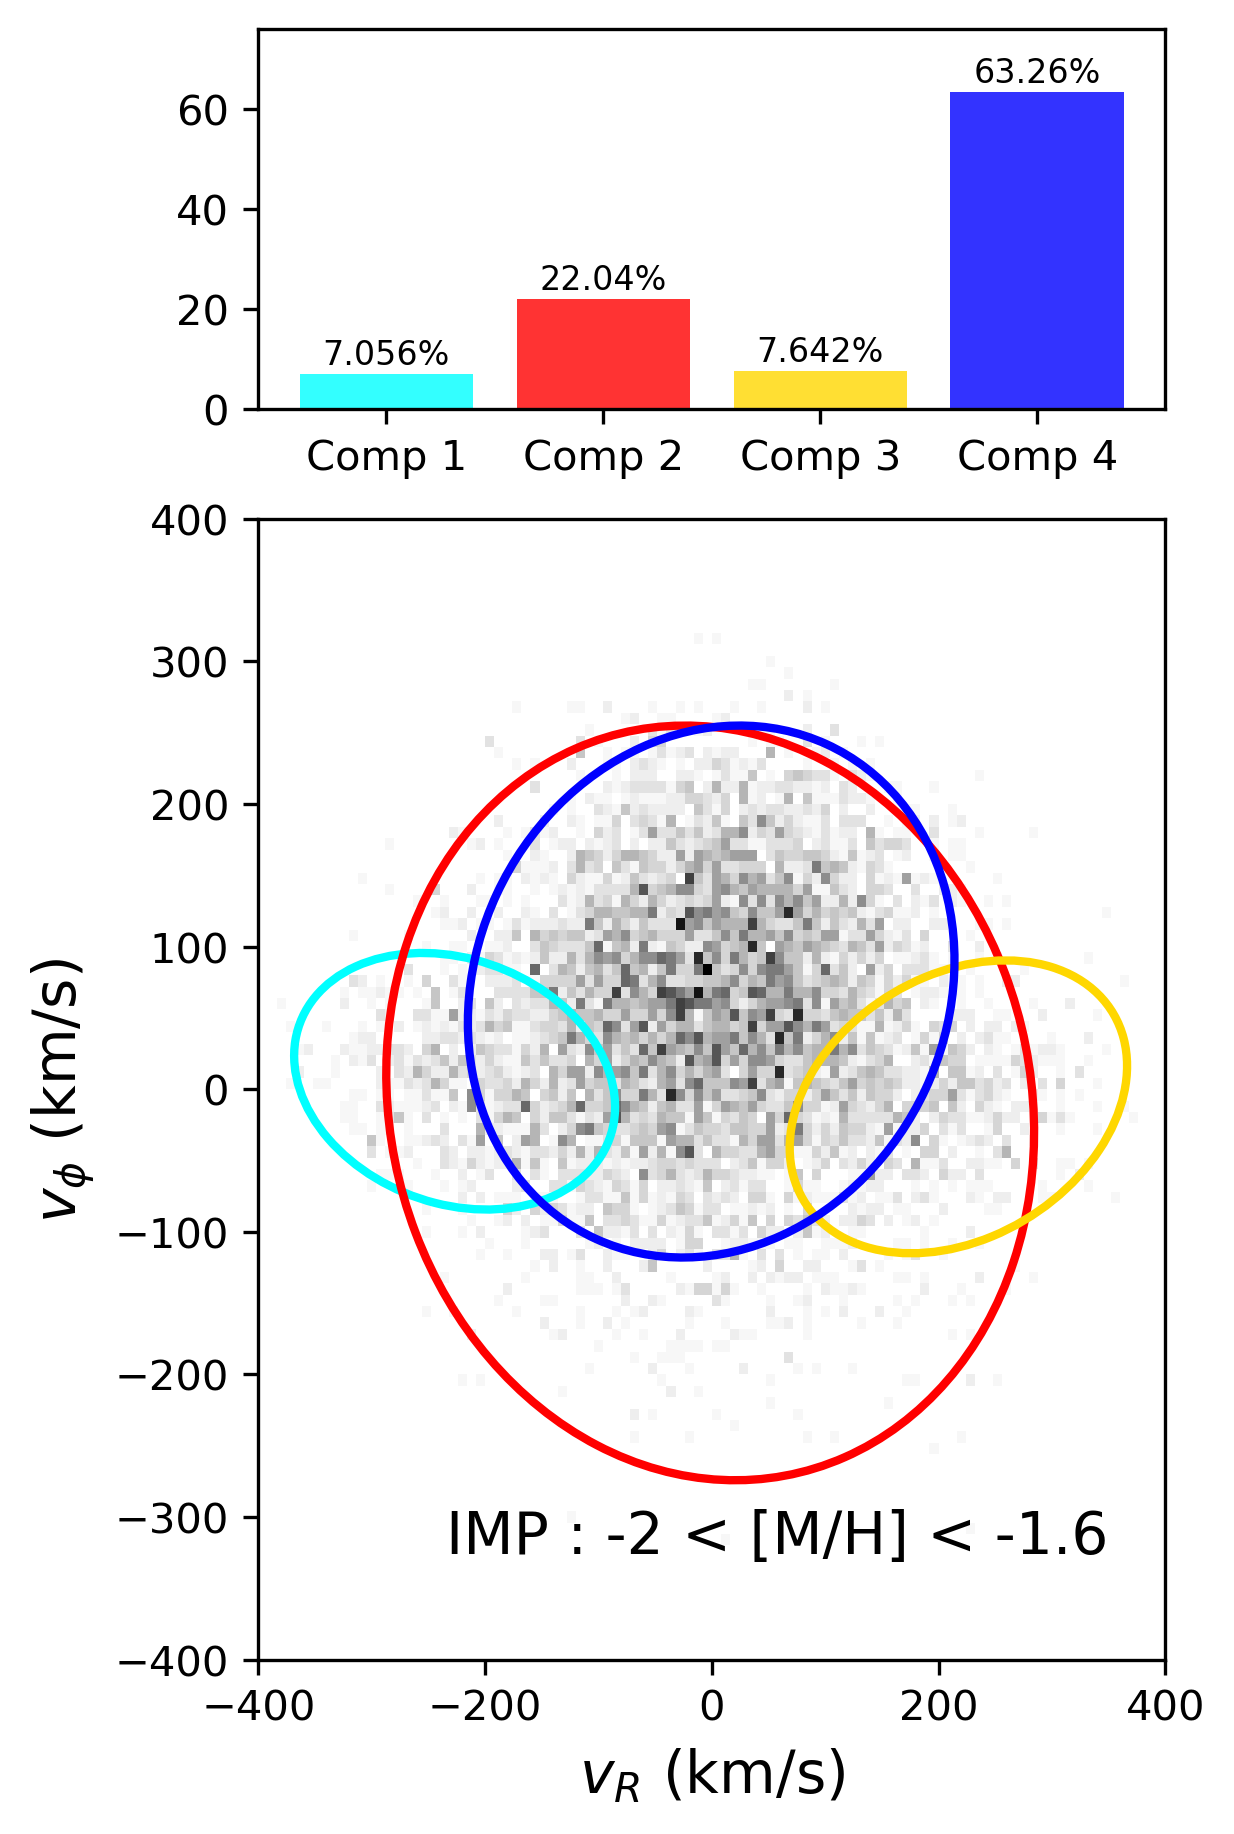
\includegraphics[width=\linewidth]{../figures/gmm_IMP.png}
    \end{subfigure}
    \hfill
    \begin{subfigure}[t]{0.24\textwidth}
        \centering
        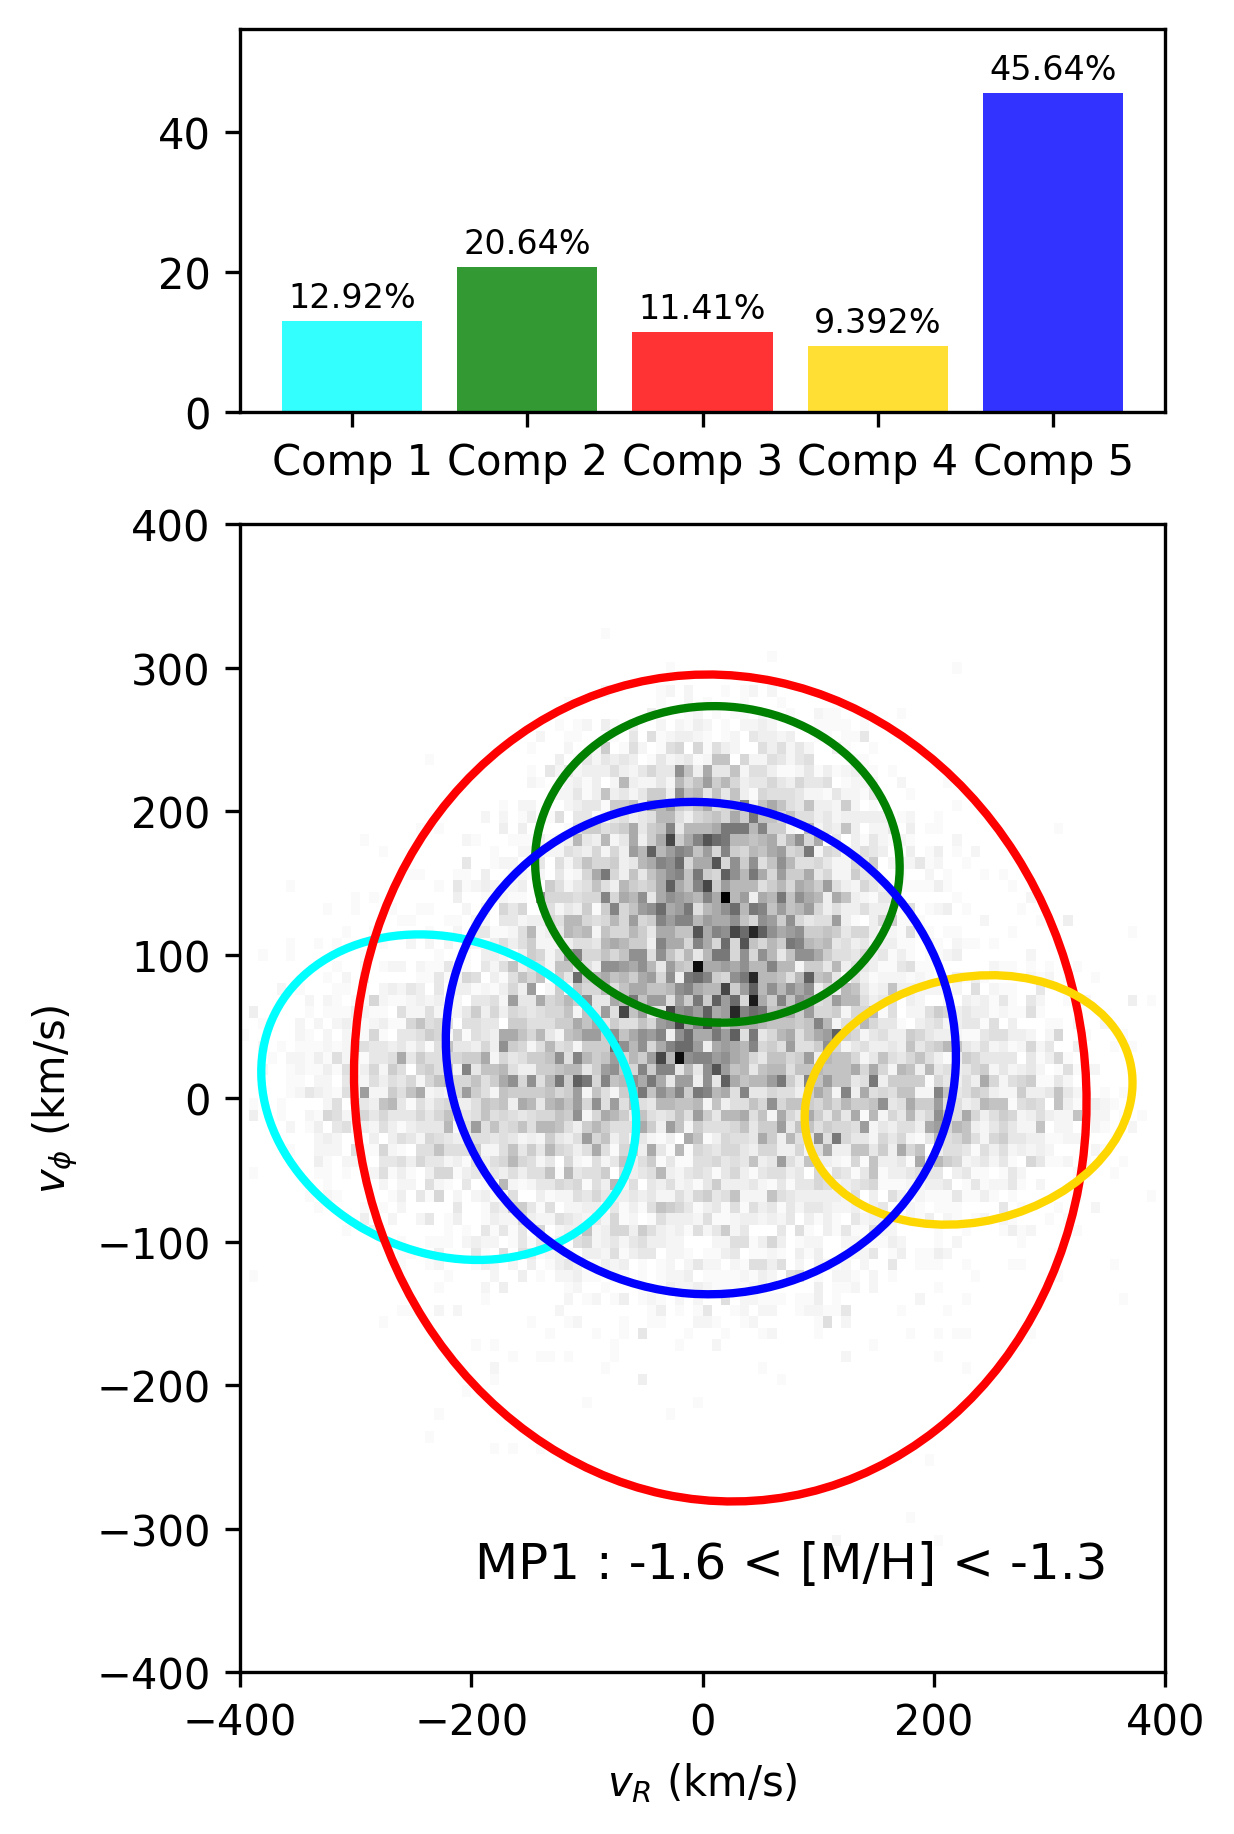
\includegraphics[width=\linewidth]{../figures/gmm_MP1.png}
    \end{subfigure}
    \hfill
    \begin{subfigure}[t]{0.24\textwidth}
        \centering
        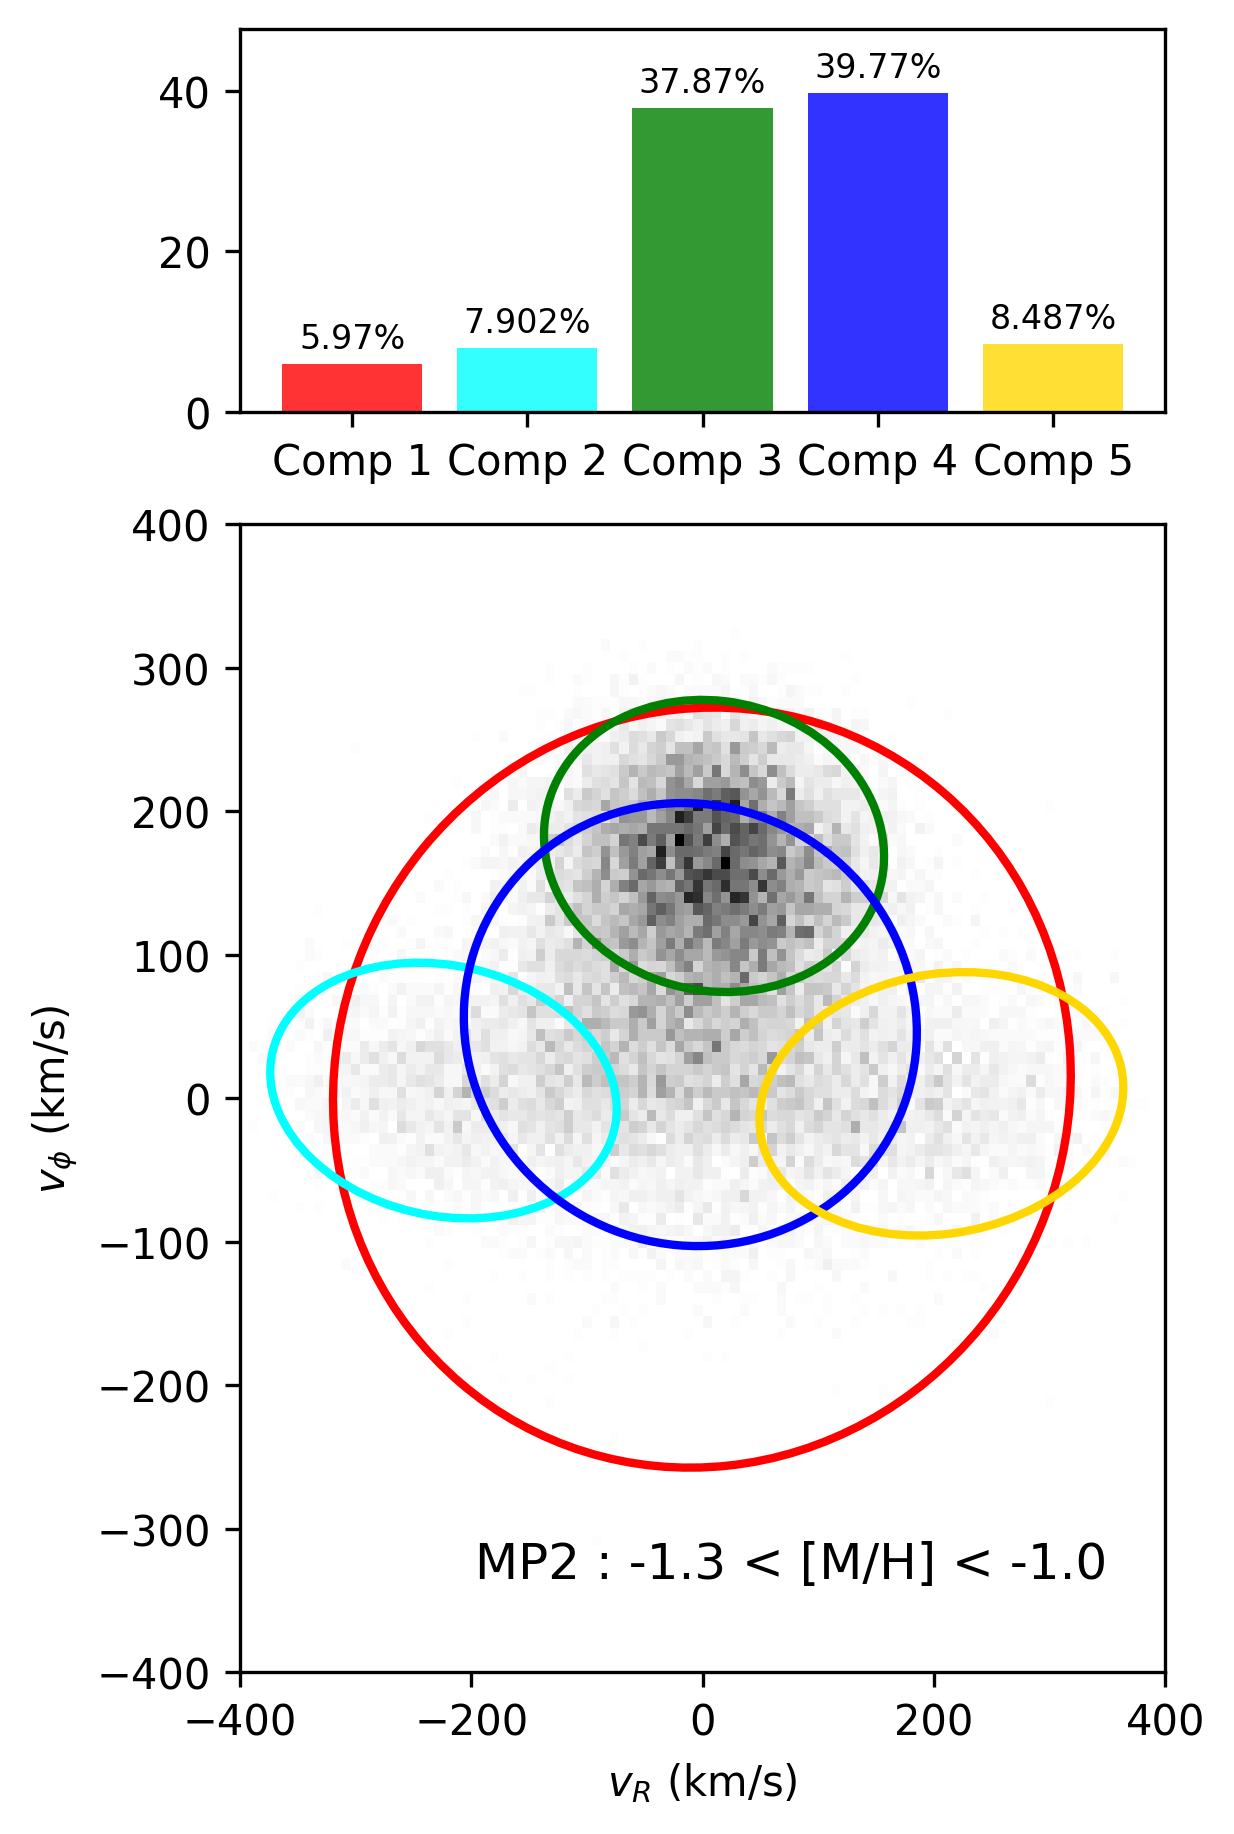
\includegraphics[width=\linewidth]{../figures/gmm_MP2.png}
    \end{subfigure}
    
    \caption{
        Gaussian Mixture Model decompositions of the stellar velocity distribution in the $v_R$–$v_\phi$ plane for each metallicity bin. 
        The bottom panel of each subfigure shows the 2D velocity distribution with GMM components overplotted as ellipses representing the 1$\sigma$ contours in $v_R$–$v_\phi$.
        The top panel shows the fractional contribution.
    }
    \label{fig:gmm_decompositions}
\end{figure*}

As shown in Figure~\ref{fig:gmm_decompositions}, the GMM is able to capture kinematic substructures in the velocity space 
of metal-poor stars. As metalicity increases, a gaussian component with a clear prograde rotation signal emerges (in green),
indiciative of a disc-like structure. The statistics of the GMM fit are summarised in Table~\ref{tab:gmm_parameters},
which lists the weights, means, and dispersions of each component in the four metallicity bins.

At $\mathrm{[M/H]} < -1.6$ (the VMP and IMP regimes), a disc component is not observed. Instead, the kinematic structure 
is dominated by a prograde halo and a stationary halo. In the VMP bin, the sample is almost evenly split between these 
two components, with the stationary halo contributing 51.1\% and the prograde halo 48.9\%. Both show broad velocity 
dispersions, with only modest rotational support ($\overline{v_\phi} \sim 69$ km\,s$^{-1}$ for the prograde halo) 
and no evidence for a kinematically cold disc-like structure.

In the IMP bin, the picture remains qualitatively similar, although the prograde halo dominates more strongly 
(63.3\%) and additional substructure becomes apparent. Two minor components, interpreted as fragments of the 
Gaia–Sausage/Enceladus (GS/E) merger debris, are also identified, each contributing $\sim$7\% of the population 
and exhibiting highly radial orbits ($|v_R| > 200$ km\,s$^{-1}$). These GS/E components are characterised by 
strong anisotropy and contribute to the broadening of the halo distribution, but again show no signature of 
disc-like kinematics. The absence of a cold, rotating disc in these bins suggests that if a very-metal-poor 
disc exists, it must be a minor contributor to the local stellar population.

Our GMM decomposition recovers the same substructures identified by \citet{zhang2024existencemetalpoordiscmilky} 
across all metallicity bins. We find similar velocity dispersions and centroid trends for the stationary halo, 
prograde halo, and GS/E components. Notably, our model assigns a more comparable weight to the 
prograde halo component in the VMP bin, in contrast to the dominant stationary 
halo reported by \citet{zhang2024existencemetalpoordiscmilky}. We also observe some variation 
in the centroid $v_\phi$ values of GS/E substructures, although their bimodal spatial structure is preserved. 

\begin{table*}
\centering
\begin{tabular}{lccccccc}
\hline
\textbf{Components} & \textbf{Weights (\%)} & $\mathbf{v_R}$ & $\boldsymbol{\sigma_R}$ & $\mathbf{v_\phi}$ & $\boldsymbol{\sigma_\phi}$ & $\mathbf{v_Z}$ & $\boldsymbol{\sigma_Z}$ \\
\hline
\multicolumn{8}{l}{\textbf{VMP:} $-3.0 < \mathrm{[M/H]} < -2.0$ (4768 stars)} \\
Stationary halo     & 51.1 & 15.86   & 143.17 &  -9.13  & 117.36 & -0.08 & 122.64 \\
Prograde halo       & 48.9 & -19.14  & 127.43 &  68.86  &  94.28 & -0.90 &  82.89 \\
\hline
\multicolumn{8}{l}{\textbf{IMP:} $-2.0 < \mathrm{[M/H]} < -1.6$ (12052 stars)} \\
Stationary halo     & 22.0 &  -1.45  & 142.88 &  -9.59  & 132.32 & -0.91 & 124.92 \\
Prograde halo       & 63.3 &  -0.58  & 107.32 &  68.52  &  93.27 & -1.16 &  72.56 \\
GS/E(1)             &  7.1 & -226.92 &  70.78 &   5.60  &  44.98 &  8.43 &  88.40 \\
GS/E(2)             &  7.6 &  217.52 &  74.41 & -12.35  &  51.35 & -4.22 &  89.78 \\
\hline
\multicolumn{8}{l}{\textbf{MP1:} $-1.6 < \mathrm{[M/H]} < -1.3$ (19142 stars)} \\
Stationary halo     & 11.3 &  15.09  & 158.68 &   7.11  & 144.33 & -2.55 & 132.08 \\
Prograde halo       & 44.5 &  -3.02  & 111.54 &  31.79  &  85.15 & -0.54 &  70.36 \\
GS/E(1)             & 12.7 & -220.40 &  80.76 &   1.01  &  56.29 &  0.47 &  91.00 \\
GS/E(2)             &  9.4 &  229.32 &  71.22 &  -0.82  &  43.42 &  1.42 &  92.69 \\
Thick disc          & 22.1 &  12.93  &  79.56 & 160.32  &  56.58 & -2.31 &  68.83 \\
\hline
\multicolumn{8}{l}{\textbf{MP2:} $-1.3 < \mathrm{[M/H]} < -1.0$ (30892 stars)} \\
Stationary halo     &  6.1 &  -1.17  & 159.06 &   8.07  & 132.05 & -3.37 & 120.46 \\
Prograde halo       & 39.4 & -13.47  &  95.65 &  53.64  &  77.86 & -3.04 &  71.00 \\
GS/E(1)             &  7.9 & -224.68 &  74.44 &   5.73  &  44.63 &  2.41 &  87.27 \\
GS/E(2)             &  9.3 &  199.71 &  81.28 &  -3.30  &  46.84 & -2.07 &  88.99 \\
Thick disc          & 37.4 &  10.56  &  73.55 & 176.07  &  50.79 &  0.85 &  62.03 \\
\hline
\end{tabular}
\caption{Parameters of the Gaussian mixture model fittings in different metallicity bins.
 The unit for all velocity columns is km\,s$^{-1}$.}
\label{tab:gmm_parameters}
\end{table*}

\subsection{Rotational Support and the Onset of Disc Formation}

To assess the degree of rotational support in each component, we compute the ratio 
$V_{\rm rot} / \sigma_\phi$, where $V_{\rm rot}$ is the mean azimuthal velocity and 
$\sigma_\phi$ its dispersion. This ratio serves as a conventional diagnostic of disc-like 
kinematics, with values $\gtrsim 3$ indicating rotation-supported populations. As shown in 
Figure~\ref{fig:v_over_sigma}, all components in the VMP and IMP bins fall below this threshold, 
confirming that the GMM identifies only dynamically hot, dispersion-supported structures in these 
regimes. This is consistent with the interpretation of the dominant components as stationary and 
prograde halo populations, with $V_{\rm rot} / \sigma_\phi \approx 0.7$ in both cases (see also 
Table~\ref{tab:gmm_parameters}).

At higher metallicities, a dynamically colder disc population emerges. In the MP1 bin, the thick 
disc component (green) rotates at $v_\phi \sim 160$ km\,s$^{-1}$ with $\sigma_\phi \sim 57$ km\,s$^{-1}$, 
yielding $V_{\rm rot} / \sigma_\phi \approx 2.8$. While just below the canonical boundary, this 
component’s low vertical dispersion and substantial weight (22.1\%) mark it as a distinct disc-like 
structure. By the MP2 bin, the disc becomes the dominant component (37.4\%), with 
$V_{\rm rot} / \sigma_\phi \approx 3.5$, indicating clear rotational support and a well-established 
thick disc. These trends point to a sharp transition in the stellar kinematics around 
$\mathrm{[M/H]} \sim -1.5$, consistent with the early onset of disc formation.

Meanwhile, the GS/E components — identifiable in the IMP, MP1, and MP2 bins — remain dynamically 
distinct, with high $|v_R|$, relatively small $v_\phi$, and negligible rotational support, reinforcing 
their origin as debris from a major radial merger \citep{Helmi2018}. Notably, given 
the estimated time of the GS/E accretion event (of order 8–11 Gyr ago \citep{Gallart2019,Belokurov2020,DiMatteo2019}),its stellar 
debris is expected to be phase-mixed. This 
implies that the positive and negative $v_R$ components should contribute approximately equally. 
This symmetry is indeed observed in the two MP bins. However, in the IMP bin the distribution is 
clearly asymmetric, with the negative $v_R$ GS/E component (aqua) containing nearly twice as many 
stars as the positive one (orange). This may suggest incomplete phase mixing or contamination by 
other structures at this intermediate metallicity.


\begin{figure}[h]
    \centering
    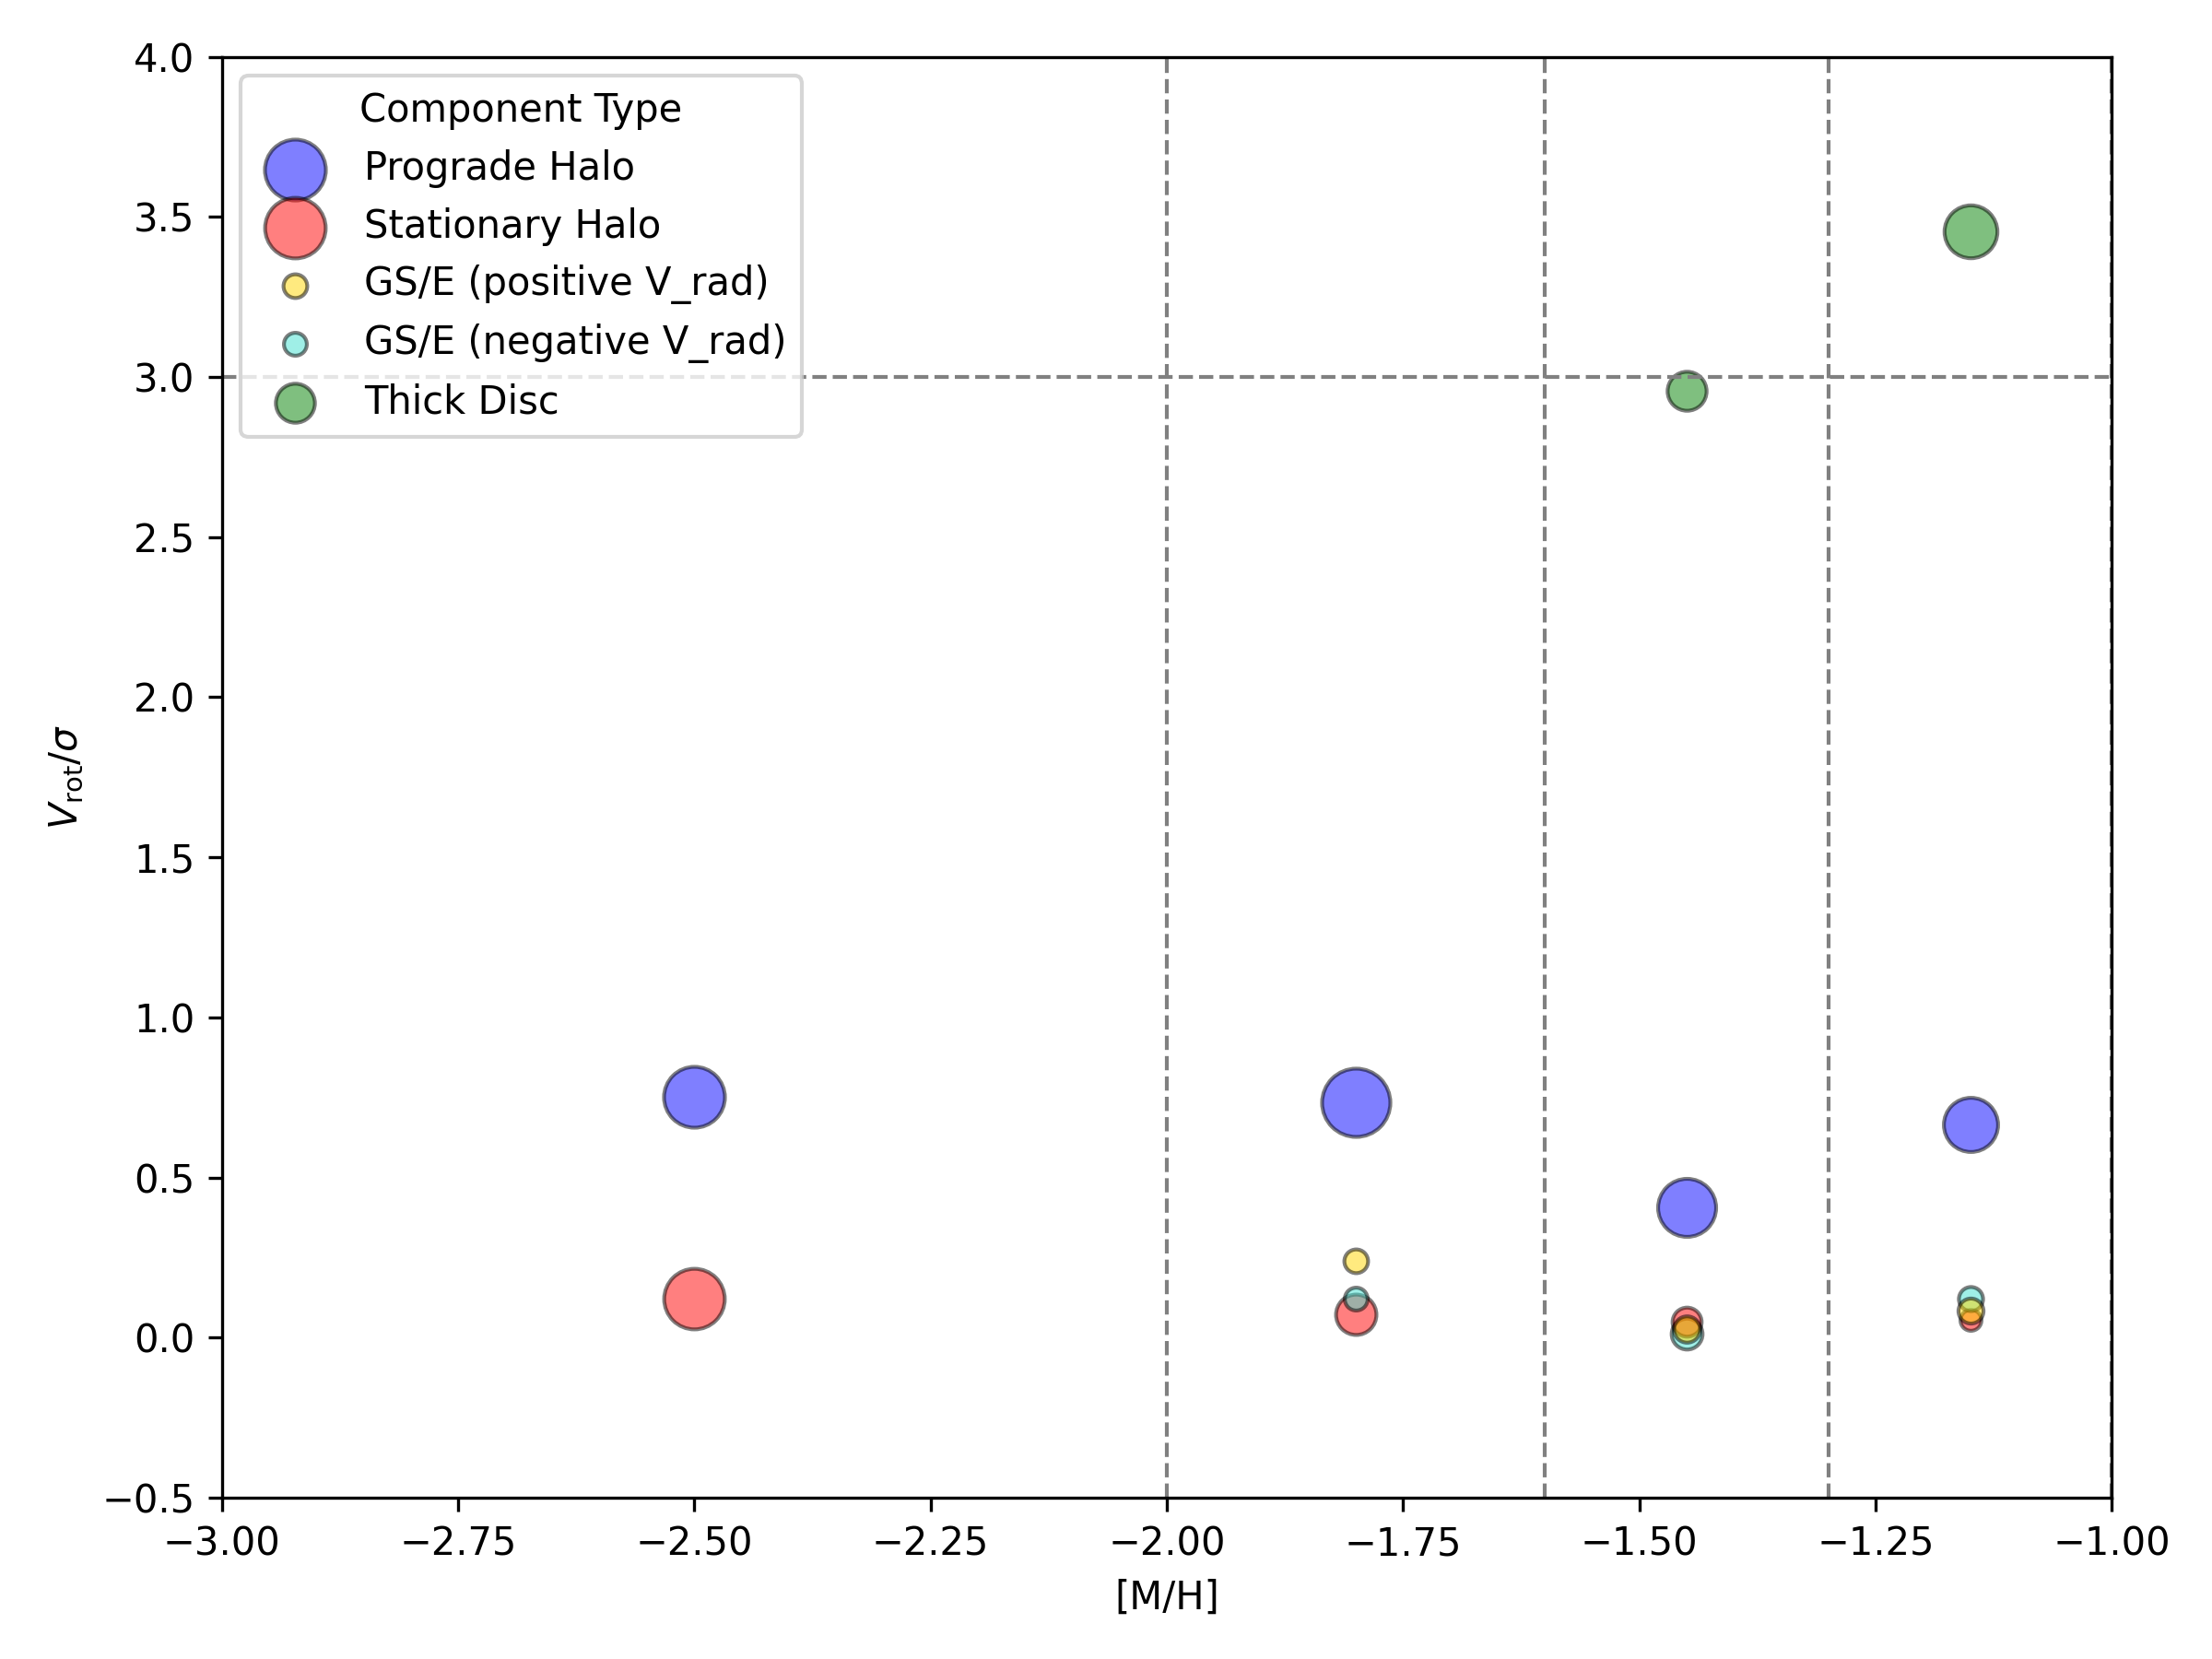
\includegraphics[width=\linewidth]{../figures/v_over_sigma_per_component.png}
    \caption{Ratio of mean rotational velocity to azimuthal velocity dispersion, $V_{\rm rot} / \sigma_\phi$, for individual GMM components in each metallicity bin. Larger squares correspond to more dominant components. Colours match the GMM components in Figure~\ref{fig:gmm_decompositions}.}
    \label{fig:v_over_sigma}
\end{figure}

\subsection{Residual Analysis for Hidden Disc Populations}

One of the limitations of GMMs is that they can fail to detect substructures that contribute 
only weakly to the overall distribution. To address this, we perform a residual analysis to test 
whether a disc-like population—too weak to be picked up by the GMM—might nonetheless be present 
in the VMP and IMP metallicity regimes.

We generated a synthetic dataset by drawing the same number of mock stars as observed stars from 
the best-fit GMM in each bin. Since our GMM uses the Extreme Deconvolution algorithm, which accounts 
for observational uncertainties during fitting, the raw samples from the model are noise-free. 
However, comparing these directly to real data would be inappropriate due to the absence of measurement 
error. To resolve this, we assign each mock star the velocity uncertainties of its nearest neighbour 
in the observed data (in $(v_R, v_\phi, v_Z)$ space), and then add Gaussian noise according to 
these uncertainties.

We then bin both the observed and mock data in the $(v_R, v_\phi)$ plane and compute the 
normalized residual map, defined as

\[
H_{\mathrm{residual}} = \frac{H_{\mathrm{obs}} - H_{\mathrm{mock}}}{H_{\mathrm{obs}} + H_{\mathrm{mock}} + \epsilon},
\]

where $H_{\mathrm{obs}}$ and $H_{\mathrm{mock}}$ are the 2D histograms and $\epsilon = 10^{-5}$ is added 
to avoid division by zero. The residual maps are shown in the top row of Figure~\ref{fig:residuals} for 
the VMP and IMP bins. The grey dashed ellipses highlight a $2\sigma$ region of a hypothetical thick disc 
with mean velocity $(v_R, v_\phi) = (0, 180)$\,km\,s$^{-1}$ and dispersions $(\sigma_R, \sigma_\phi) 
= (70, 50)$\,km\,s$^{-1}$, consistent with the thick disc component seen in the MP2 metallicity bin.

To quantify the possible presence of a hidden disc, we count the excess number of observed stars inside 
this thick disc ellipse relative to the GMM-generated sample. We repeat this calculation for 200 Monte 
Carlo realizations to estimate the residual and its uncertainty. The results are shown as horizontal 
dashed lines in the bottom row of Figure~\ref{fig:residuals}, representing a disc-like residual 
of $40.4 \pm 24.8$ stars in the VMP bin and $76.9 \pm 42.8$ stars in the IMP bin.

To interpret these residuals, we repeat the same procedure but now inject a mock disc population—
generated from the same thick disc Gaussian—into the GMM baseline. By varying the injected disc 
fraction from 0\% to 5\% of the sample and recalculating the residual each time, we construct a 
relationship between disc fraction and expected residual. This is shown as the solid black line in the 
bottom panels of Figure~\ref{fig:residuals}, with the red shaded region indicating the $1\sigma$ 
uncertainty across Monte Carlo trials.

\begin{figure}[ht]
    \centering
    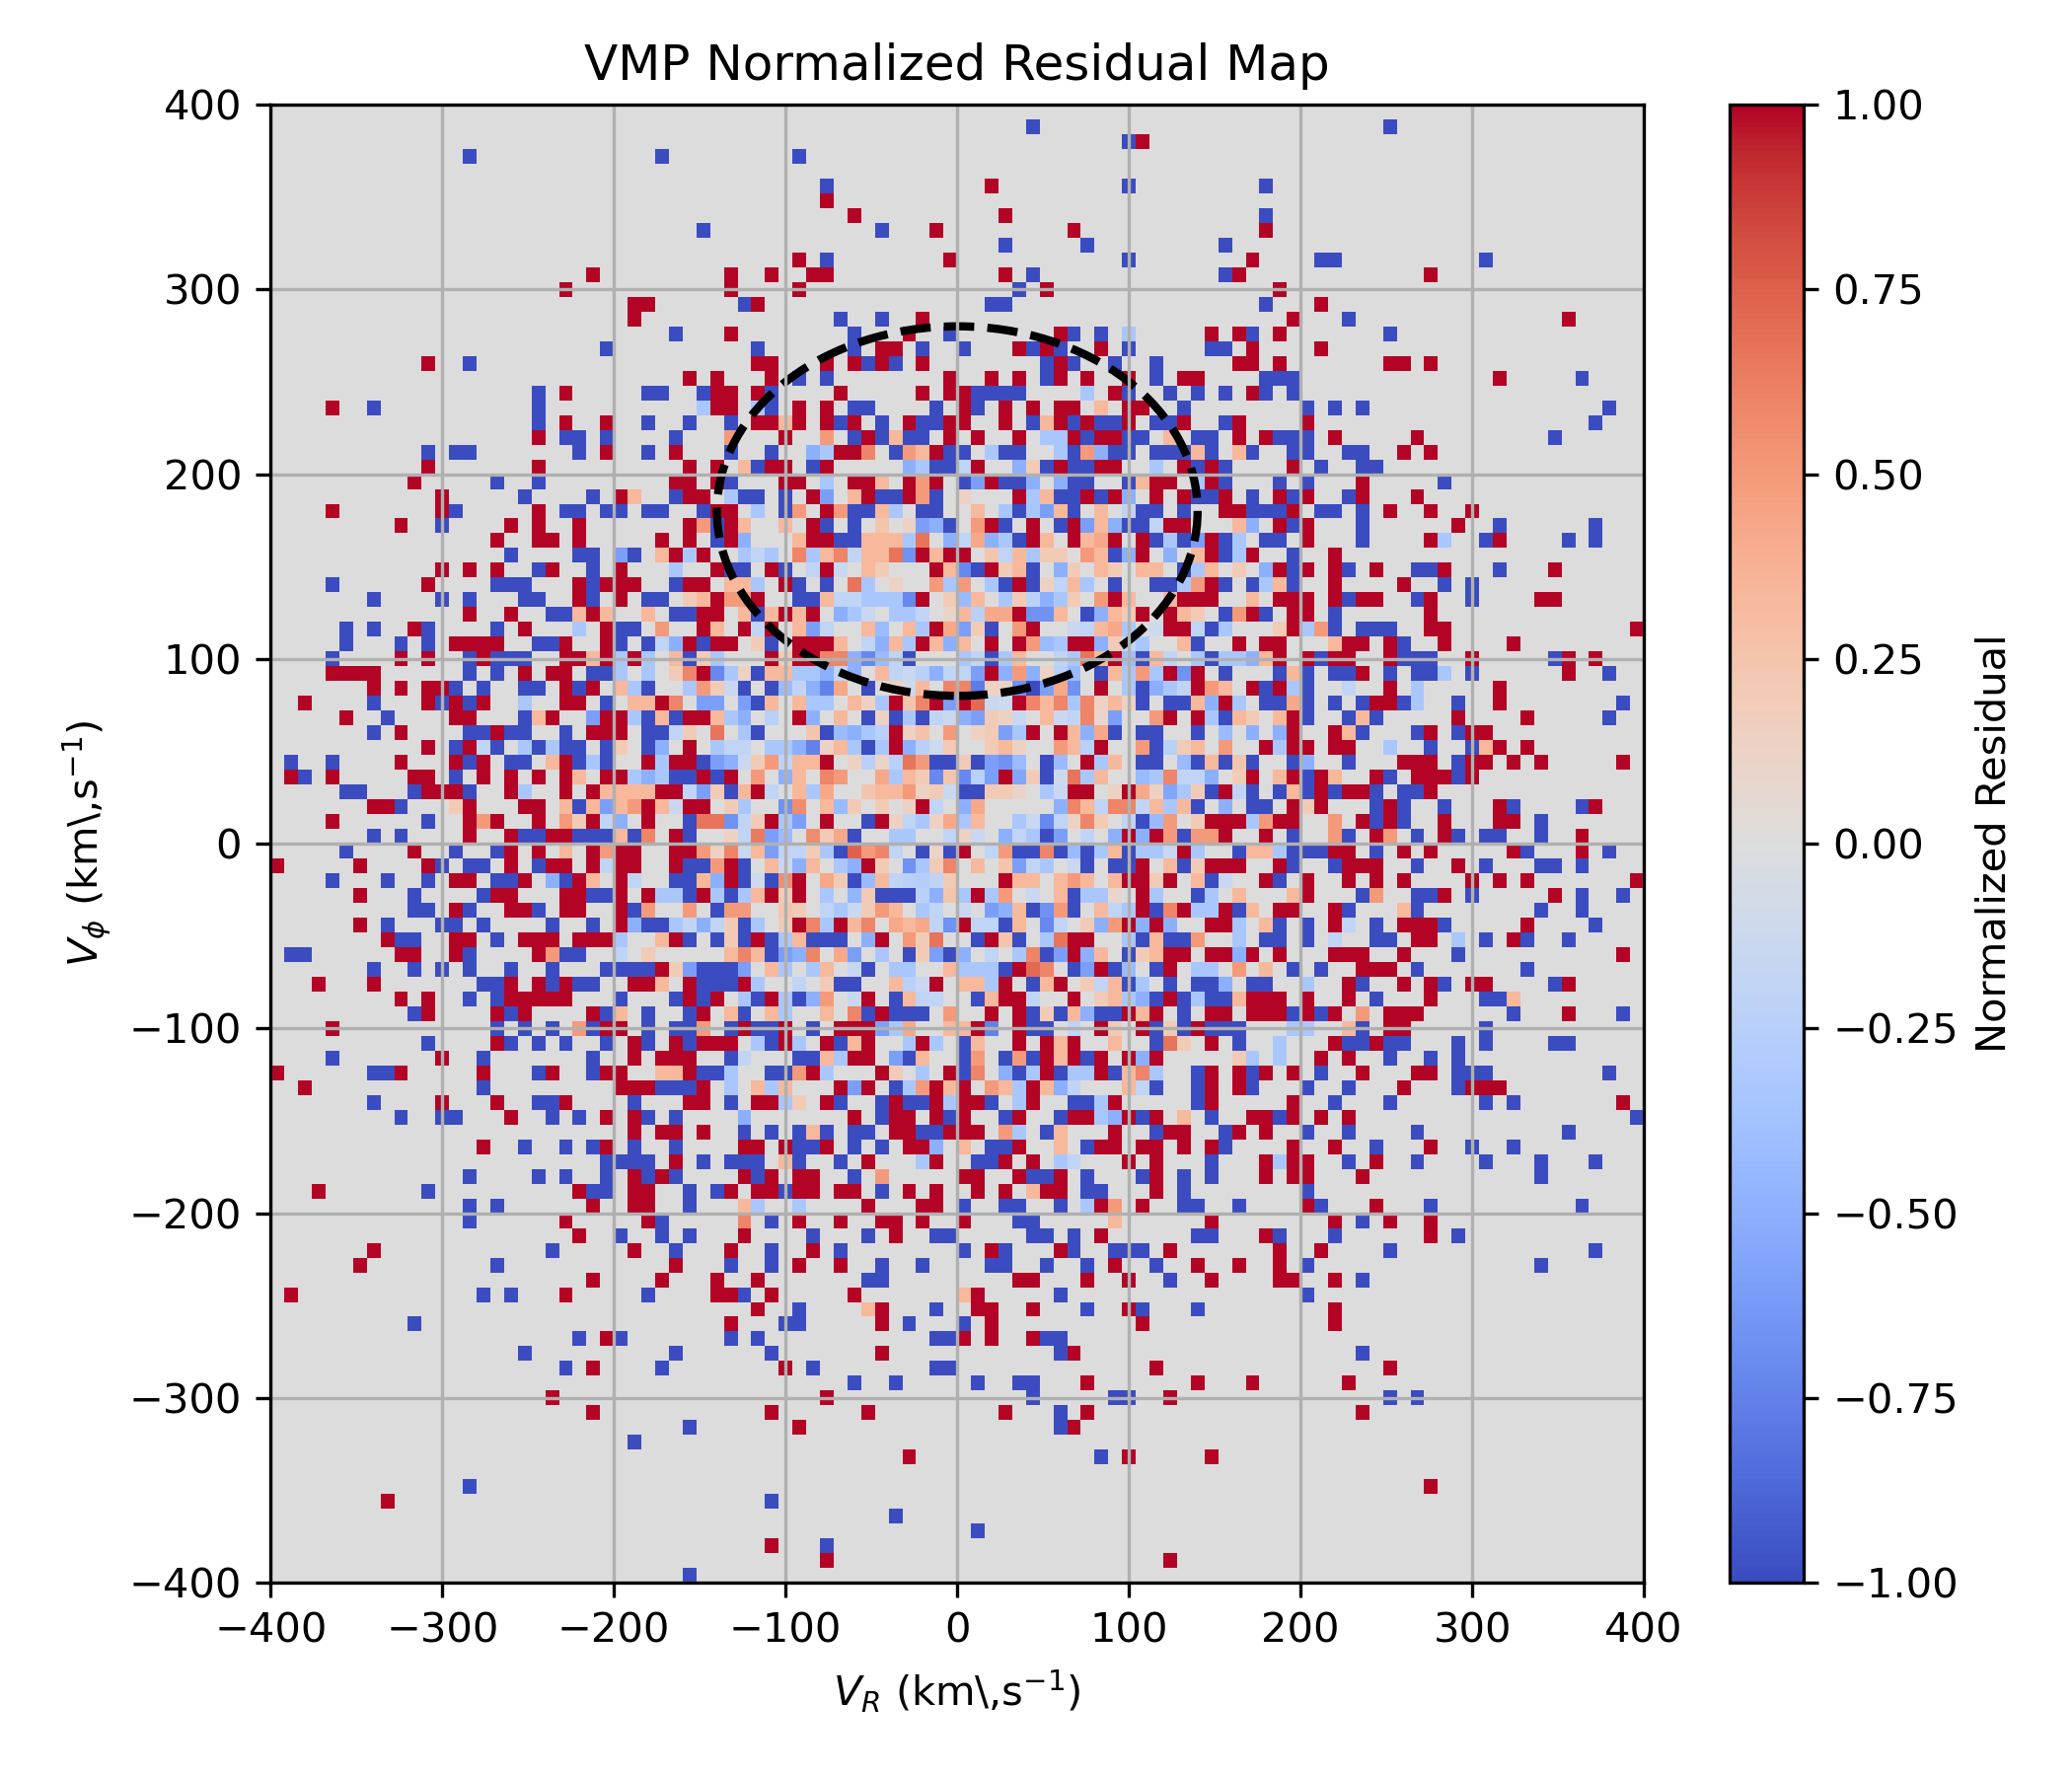
\includegraphics[width=0.49\textwidth]{../figures/vmp_residual_map.png}
    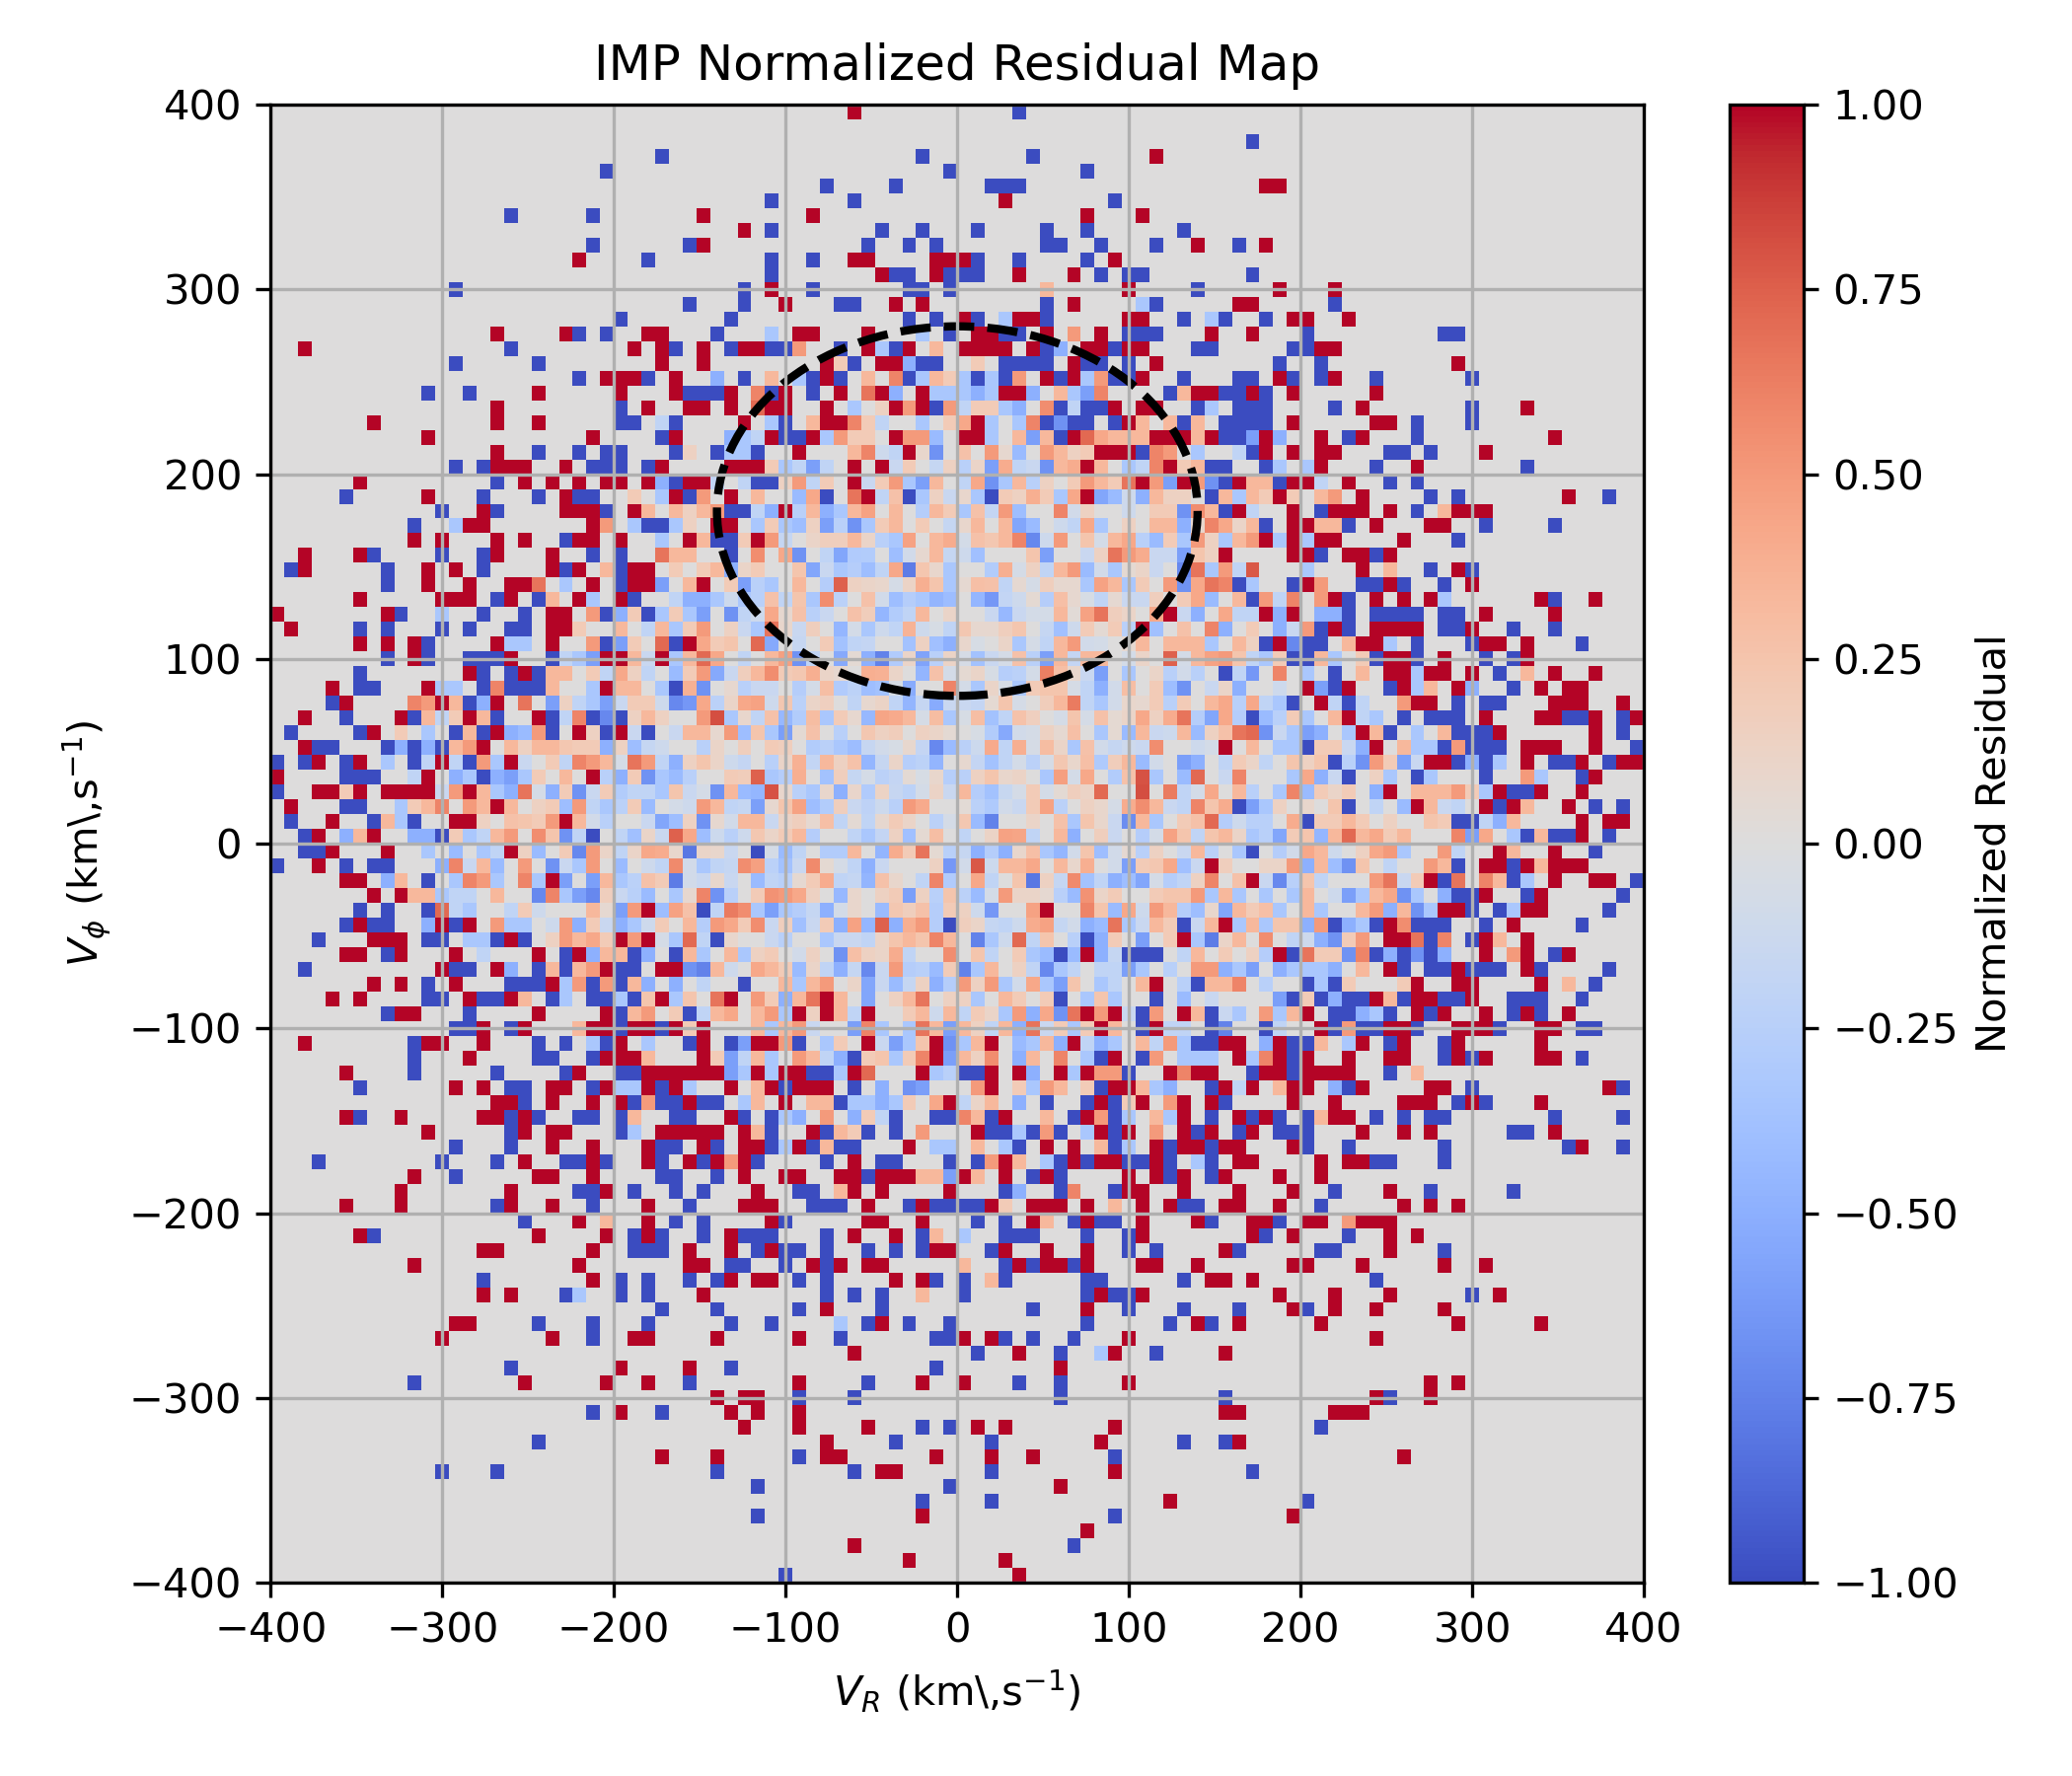
\includegraphics[width=0.49\textwidth]{../figures/imp_residual_map.png} \\
    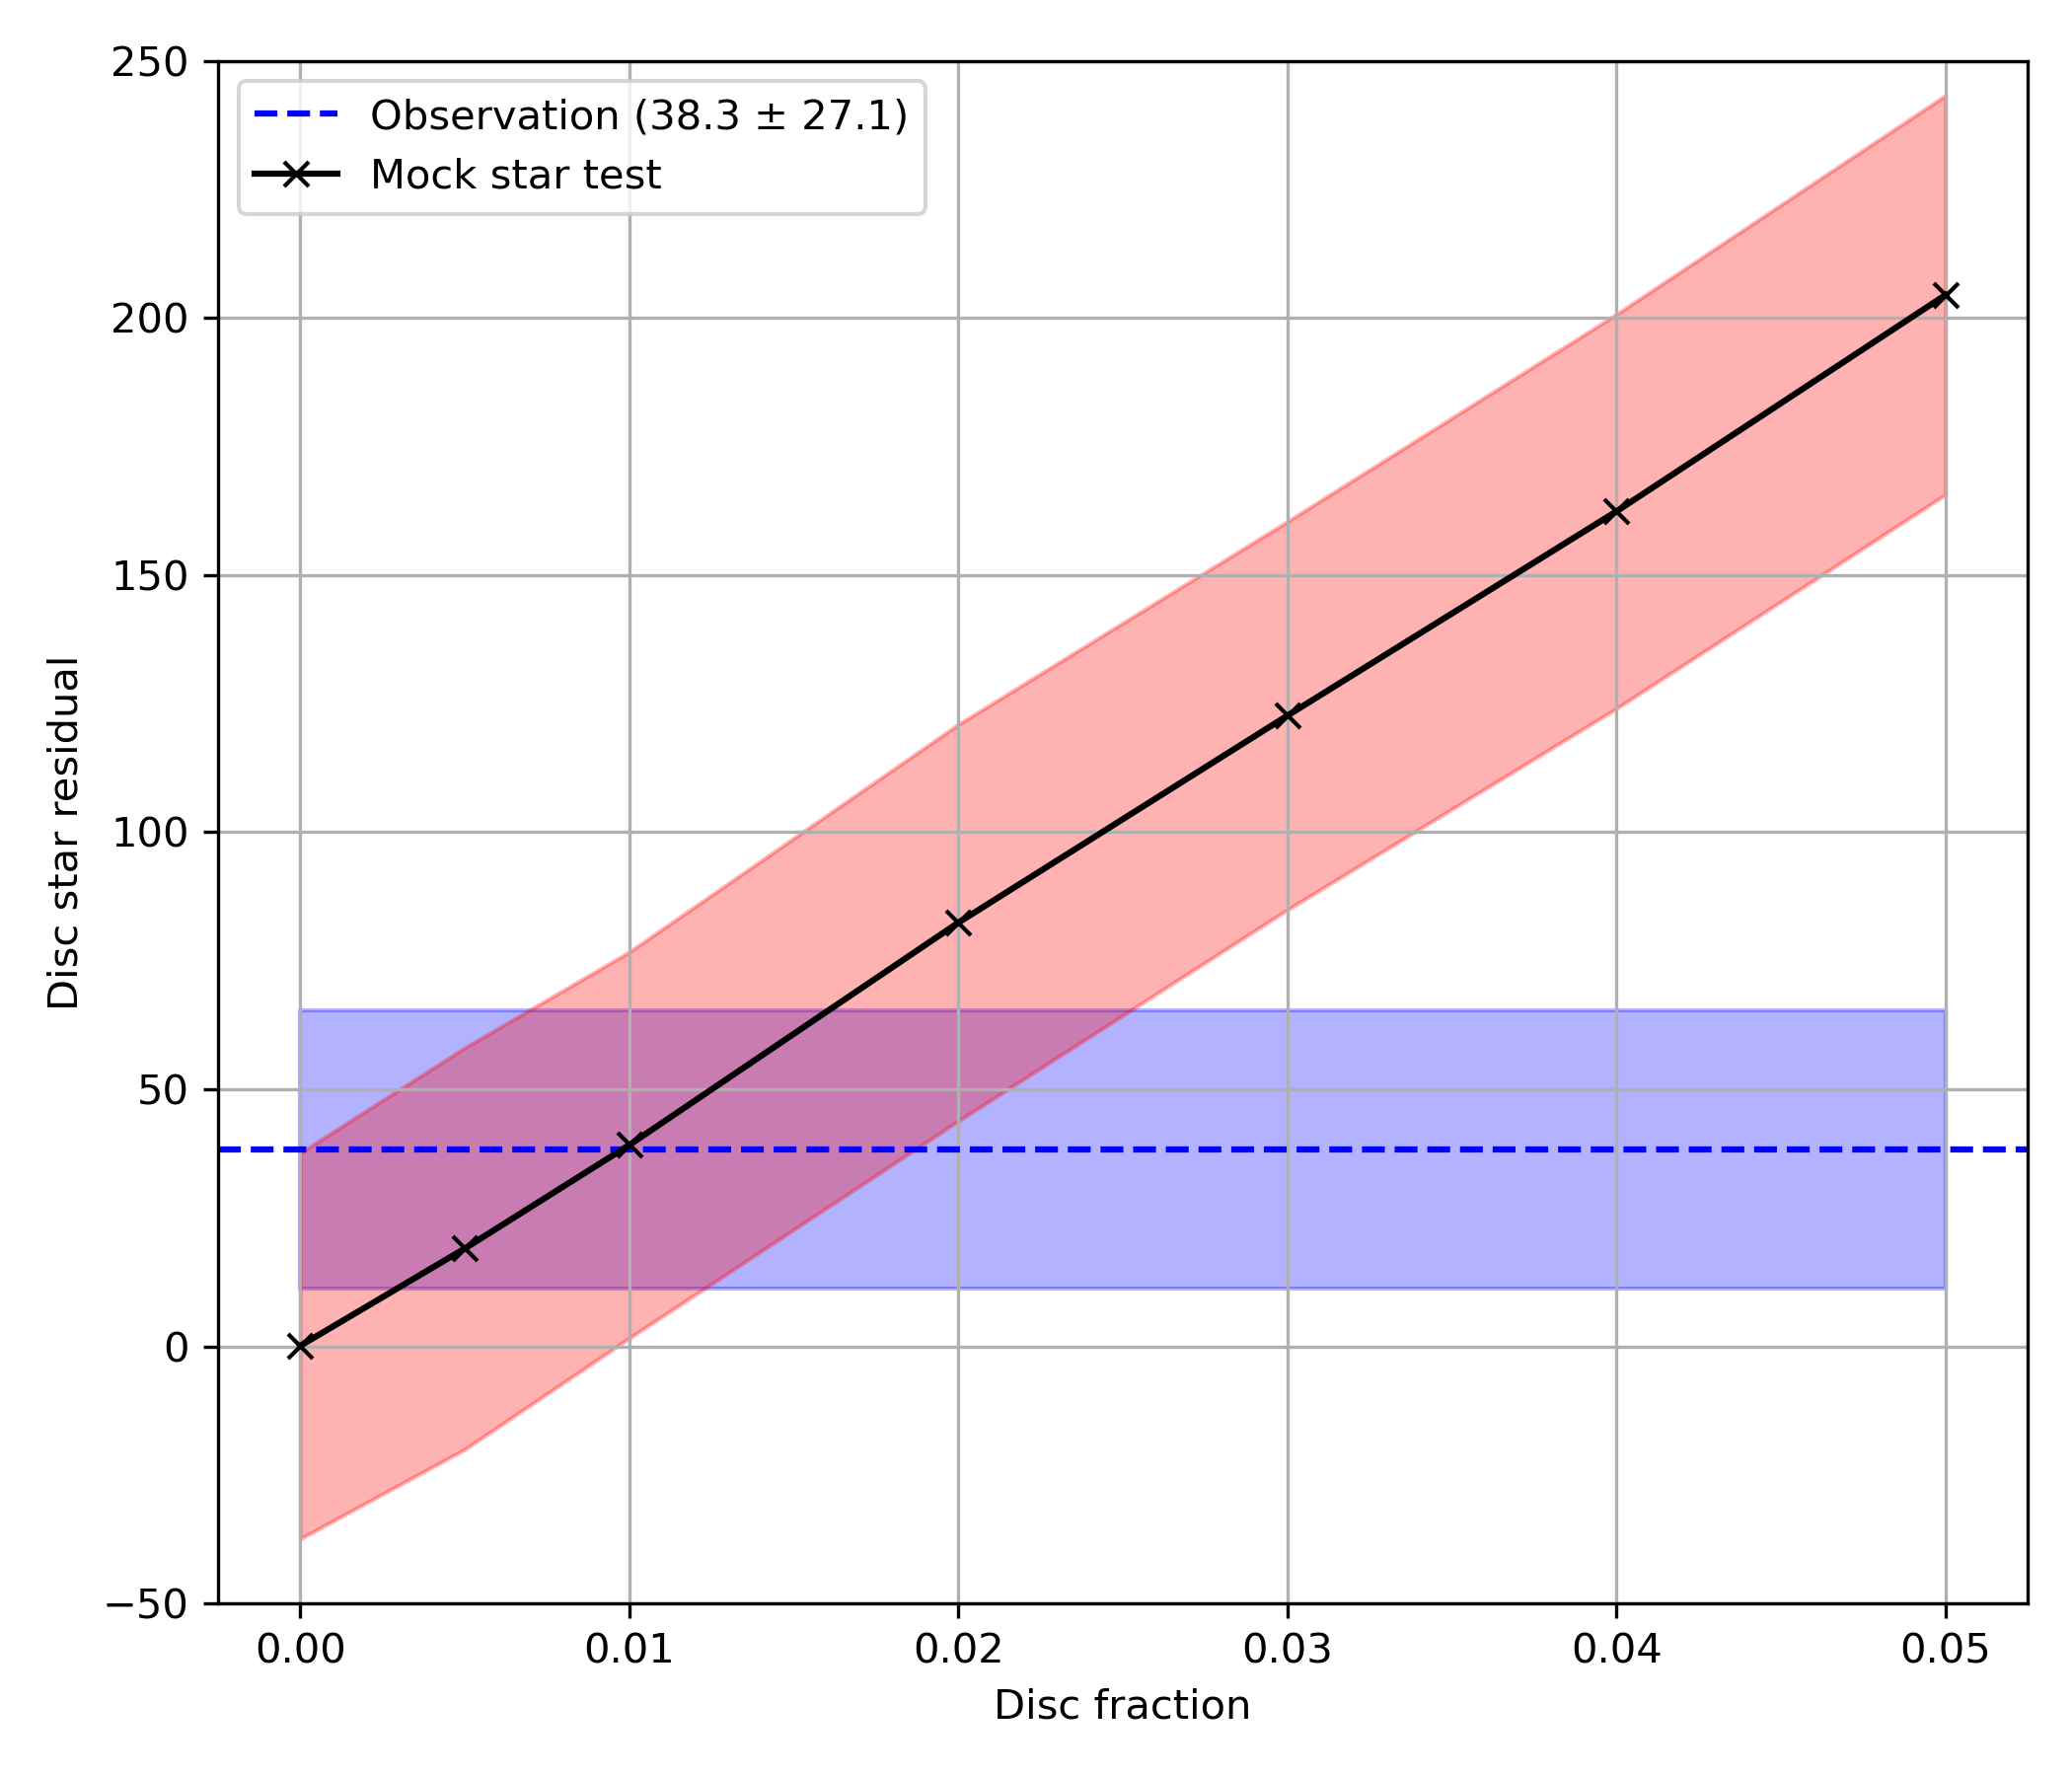
\includegraphics[width=0.49\textwidth]{../figures/vmp_disc_fraction.png}
    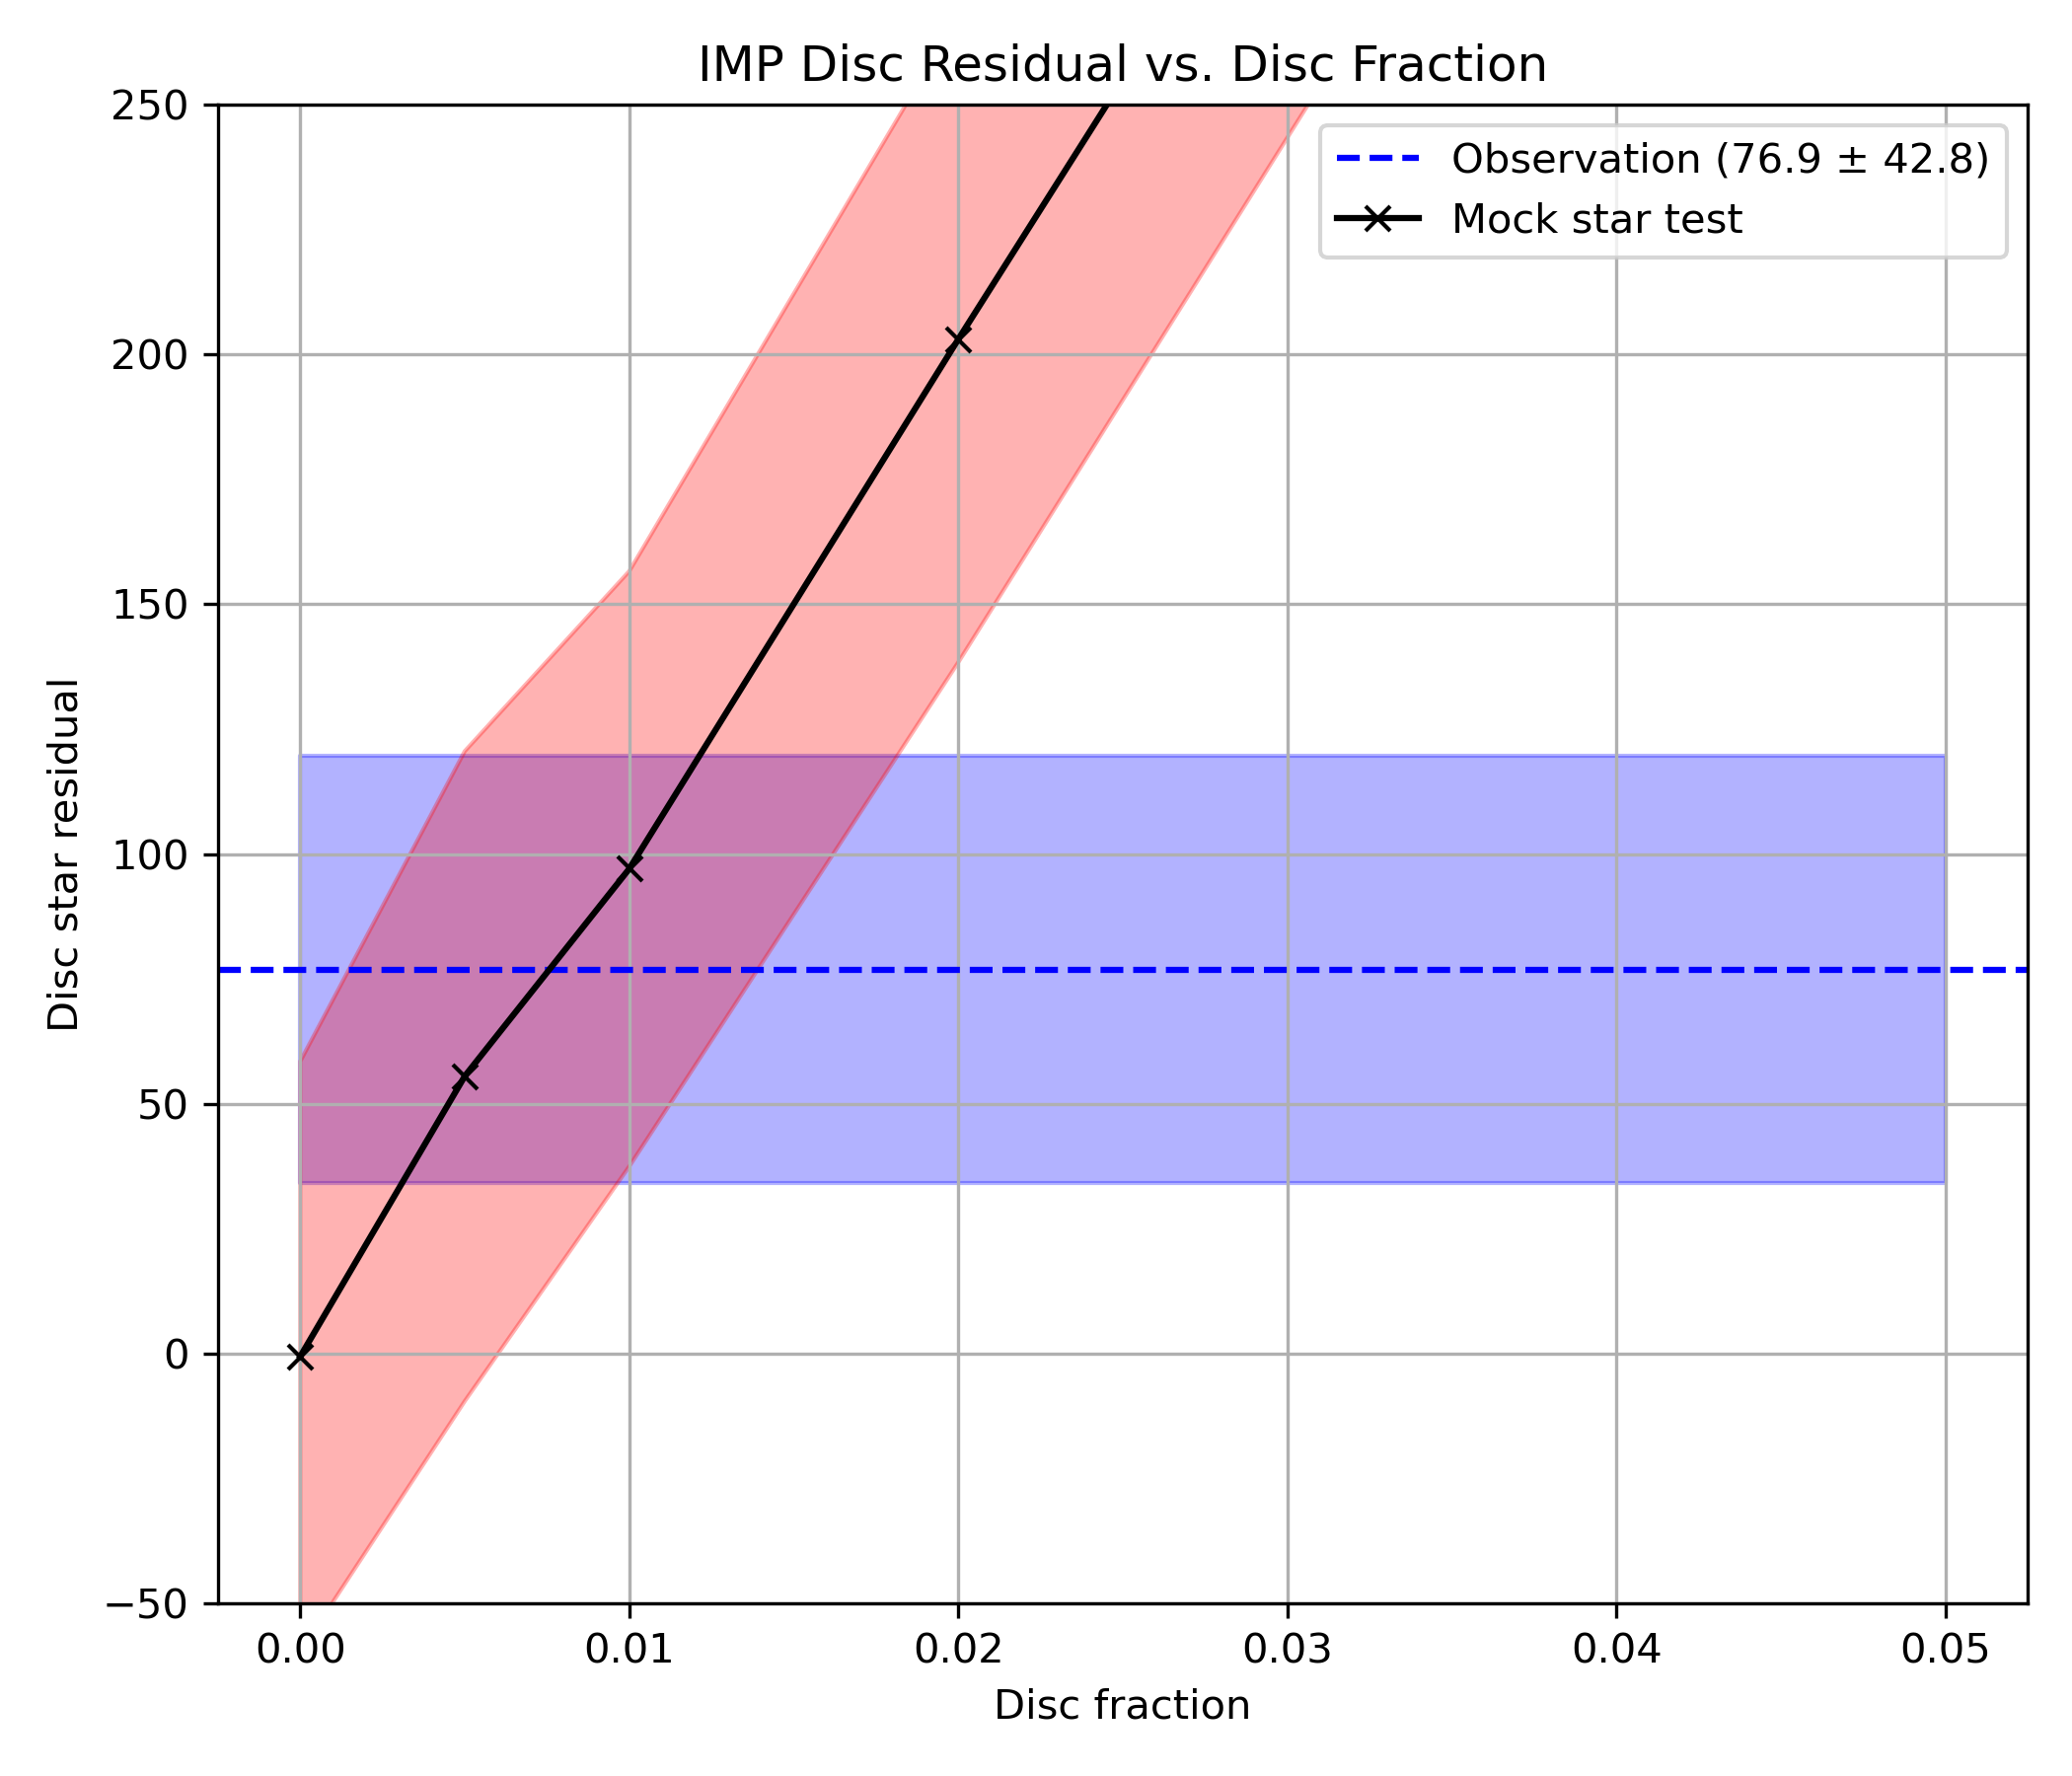
\includegraphics[width=0.49\textwidth]{../figures/imp_disc_fraction.png}
    \caption{Top: Normalized residual maps between observed and GMM-predicted velocity distributions in $(v_R, v_\phi)$ for the VMP (left) and IMP (right) metallicity bins. Grey ellipses show the $2\sigma$ contour of the fiducial thick disc model. Bottom: Disc residuals as a function of injected disc fraction. The dashed line and blue band indicate the observed residual and its uncertainty. The solid black line and red region show mock test results and their uncertainties.}
    \label{fig:residuals}
\end{figure}


\section{Extension analysis}
\subsection{Alpha–element abundance}\label{subsec:alpha}

We extend the chemo–kinematic analysis by adding the
alpha-to-iron ratio $[\alpha/\mathrm{Fe}]$, where the “alpha’’ elements
(O, Ne, Mg, Si, S, Ca, Ti) are produced almost entirely in core–collapse
(\hbox{Type II}) supernovae, whereas most iron is released later by
thermonuclear (Type Ia) explosions.  Because the two channels operate on
very different time-scales—$\sim$10–30 Myr for Type II versus
$\gtrsim$\,0.1–1 Gyr for Type Ia—the quantity $[\alpha/\mathrm{Fe}]$
encodes the star-formation history of a stellar population:

\begin{itemize}
  \item \textbf{High $[\alpha/\mathrm{Fe}]$.}  
      Rapid, intense star formation enriches gas with $\alpha$-elements 
      before significant iron production from Type Ia supernovae occurs, 
      leading to elevated $[\alpha/\mathrm{Fe}]$. This chemical signature is typical 
      of the in-situ thick disc, stellar halo, and some ancient accreted material. 
      However, at fixed metallicity, accreted populations, especially dwarf galaxies,
       tend to show lower $[\alpha/\mathrm{Fe}]$ 
      compared to in-situ stars, reflecting their slower chemical evolution.


  \item \textbf{Low $[\alpha/\mathrm{Fe}]$.}  
        A more prolonged formation history allowed Type Ia ejecta to
        accumulate, diluting the alpha enhancement.  The present-day thin
        disc and metal-rich bulge occupy this regime.
\end{itemize}

Hence the $[\alpha/\mathrm{Fe}]$–$[\mathrm{M/H}]$ plane acts as a chemical
clock: populations that overlap in $[\mathrm{M/H}]$ but differ in formation
time-scale separate cleanly in $[\alpha/\mathrm{Fe}]$.

Following \citet{Vis2024}, we separate the RGB catalogue into
high- and low-$[\alpha/{\rm M}]$ sequences using the XP abundances of
\citet{Li2024} and model each subset with an error–convolved
Gaussian–mixture as described earlier.  Before fitting the GMM,
we can expect to see some differences between the high- and low-$[\alpha/{\rm M}]$ sequences
as summarised below.  

In the high-$[\alpha/{\rm M}]$ sequence, the oldest, in-situ population formed rapidly from well-mixed,
$\alpha$-rich gas. Below $[\mathrm{M/H}]\!\approx\!-1.6$ we therefore
expect a single non-rotating halo Gaussian.  As enrichment proceeds,
gas spins up and produces the thick disc: a prograde, kinematically
warm Gaussian whose weight rises steeply between
$[\mathrm{M/H}]\!\simeq\!-1.6$ and $-1.0$ and dominates for
$[\mathrm{M/H}]>-0.7$.  Accreted debris from the last major merger
(Gaia–Sausage/Enceladus, GS/E) should not be prominent here
because GS/E stars are typically \emph{less} $\alpha$-enhanced than the
in-situ thick disc at the same metallicity
\citep[e.g.][]{Helmi2018}; our conservative
high-$[\alpha/{\rm M}]$ cut should remove most of this material.

In the low-$[\alpha/{\rm M}]$ sequence,
lower $[\alpha/{\rm M}]$ signals slower enrichment, typical of dwarf
satellites or the Milky Way disc after Type-Ia supernovae began adding
iron.  A single halo Gaussian should suffice below
$[\mathrm{M/H}]\!\approx\!-1.3$, with a cold, high-weight thin-disc
Gaussian—centred near the Local Standard of Rest and
$\sigma\!\lesssim\!30\;\mathrm{km\,s^{-1}}$—emerging above that
threshold.  Our footprint excludes $|b|<10^{\circ}$, however, and thus
removes most of the geometrically thin disc; the ultra-cold Gaussian
may therefore be absent at the low metalicities we are inspecting. 
 The aim is instead to pinpoint the onset
of disc-like rotation in the low-$[\alpha/{\rm M}]$ sequence despite
this selection bias.





\subsection{Data}


We obtain the $\alpha$-to-metal abundance ratios from the
XP–based catalogue of \citet{Li2024}, whose neural-network
model, trained on high-resolution \textsc{APOGEE}~DR17
spectra, achieves a typical precision of $\simeq0.05$\,dex for
bright sources ($G<16$).  
Following \citet{Vis2024}, we cross-match the XP-based $\alpha$ catalogue 
of \citet{Li2024} with the metallicity-selected red-giant branch sample . This base sample already 
incorporates the red-giant selection and photometric quality cuts from 
\citet{Andrae2023}, including limits on surface gravity, colour–magnitude 
position, and XP calibration reliability. 

To further ensure robust $\alpha$ abundances and kinematics, we apply 
several additional cuts:
\begin{itemize}\setlength\itemsep{2pt}
  \item we reject stars within $1^\circ$ of known dwarf galaxies and 
        those associated with globular clusters;
  \item a reddening cut $E(B-V)<0.5$ removes stars in regions of high 
        extinction, where XP abundances are less reliable;
  \item a Galactic latitude cut $|b|>10^\circ$ similarly avoids 
        the dust-dominated plane;
  \item we relax the fractional parallax uncertainty cut relative to 
        Section~\ref{subsec:data_sample}, requiring only $\mathrm{fpu}<0.2$
        to retain sufficient stars in the metal-poor regime, which is 
        the focus of this analysis.
\end{itemize}


We obtain approximately 3.4 million stars in our final sample with alpha element abundances.

\begin{figure}[h]
    \centering
    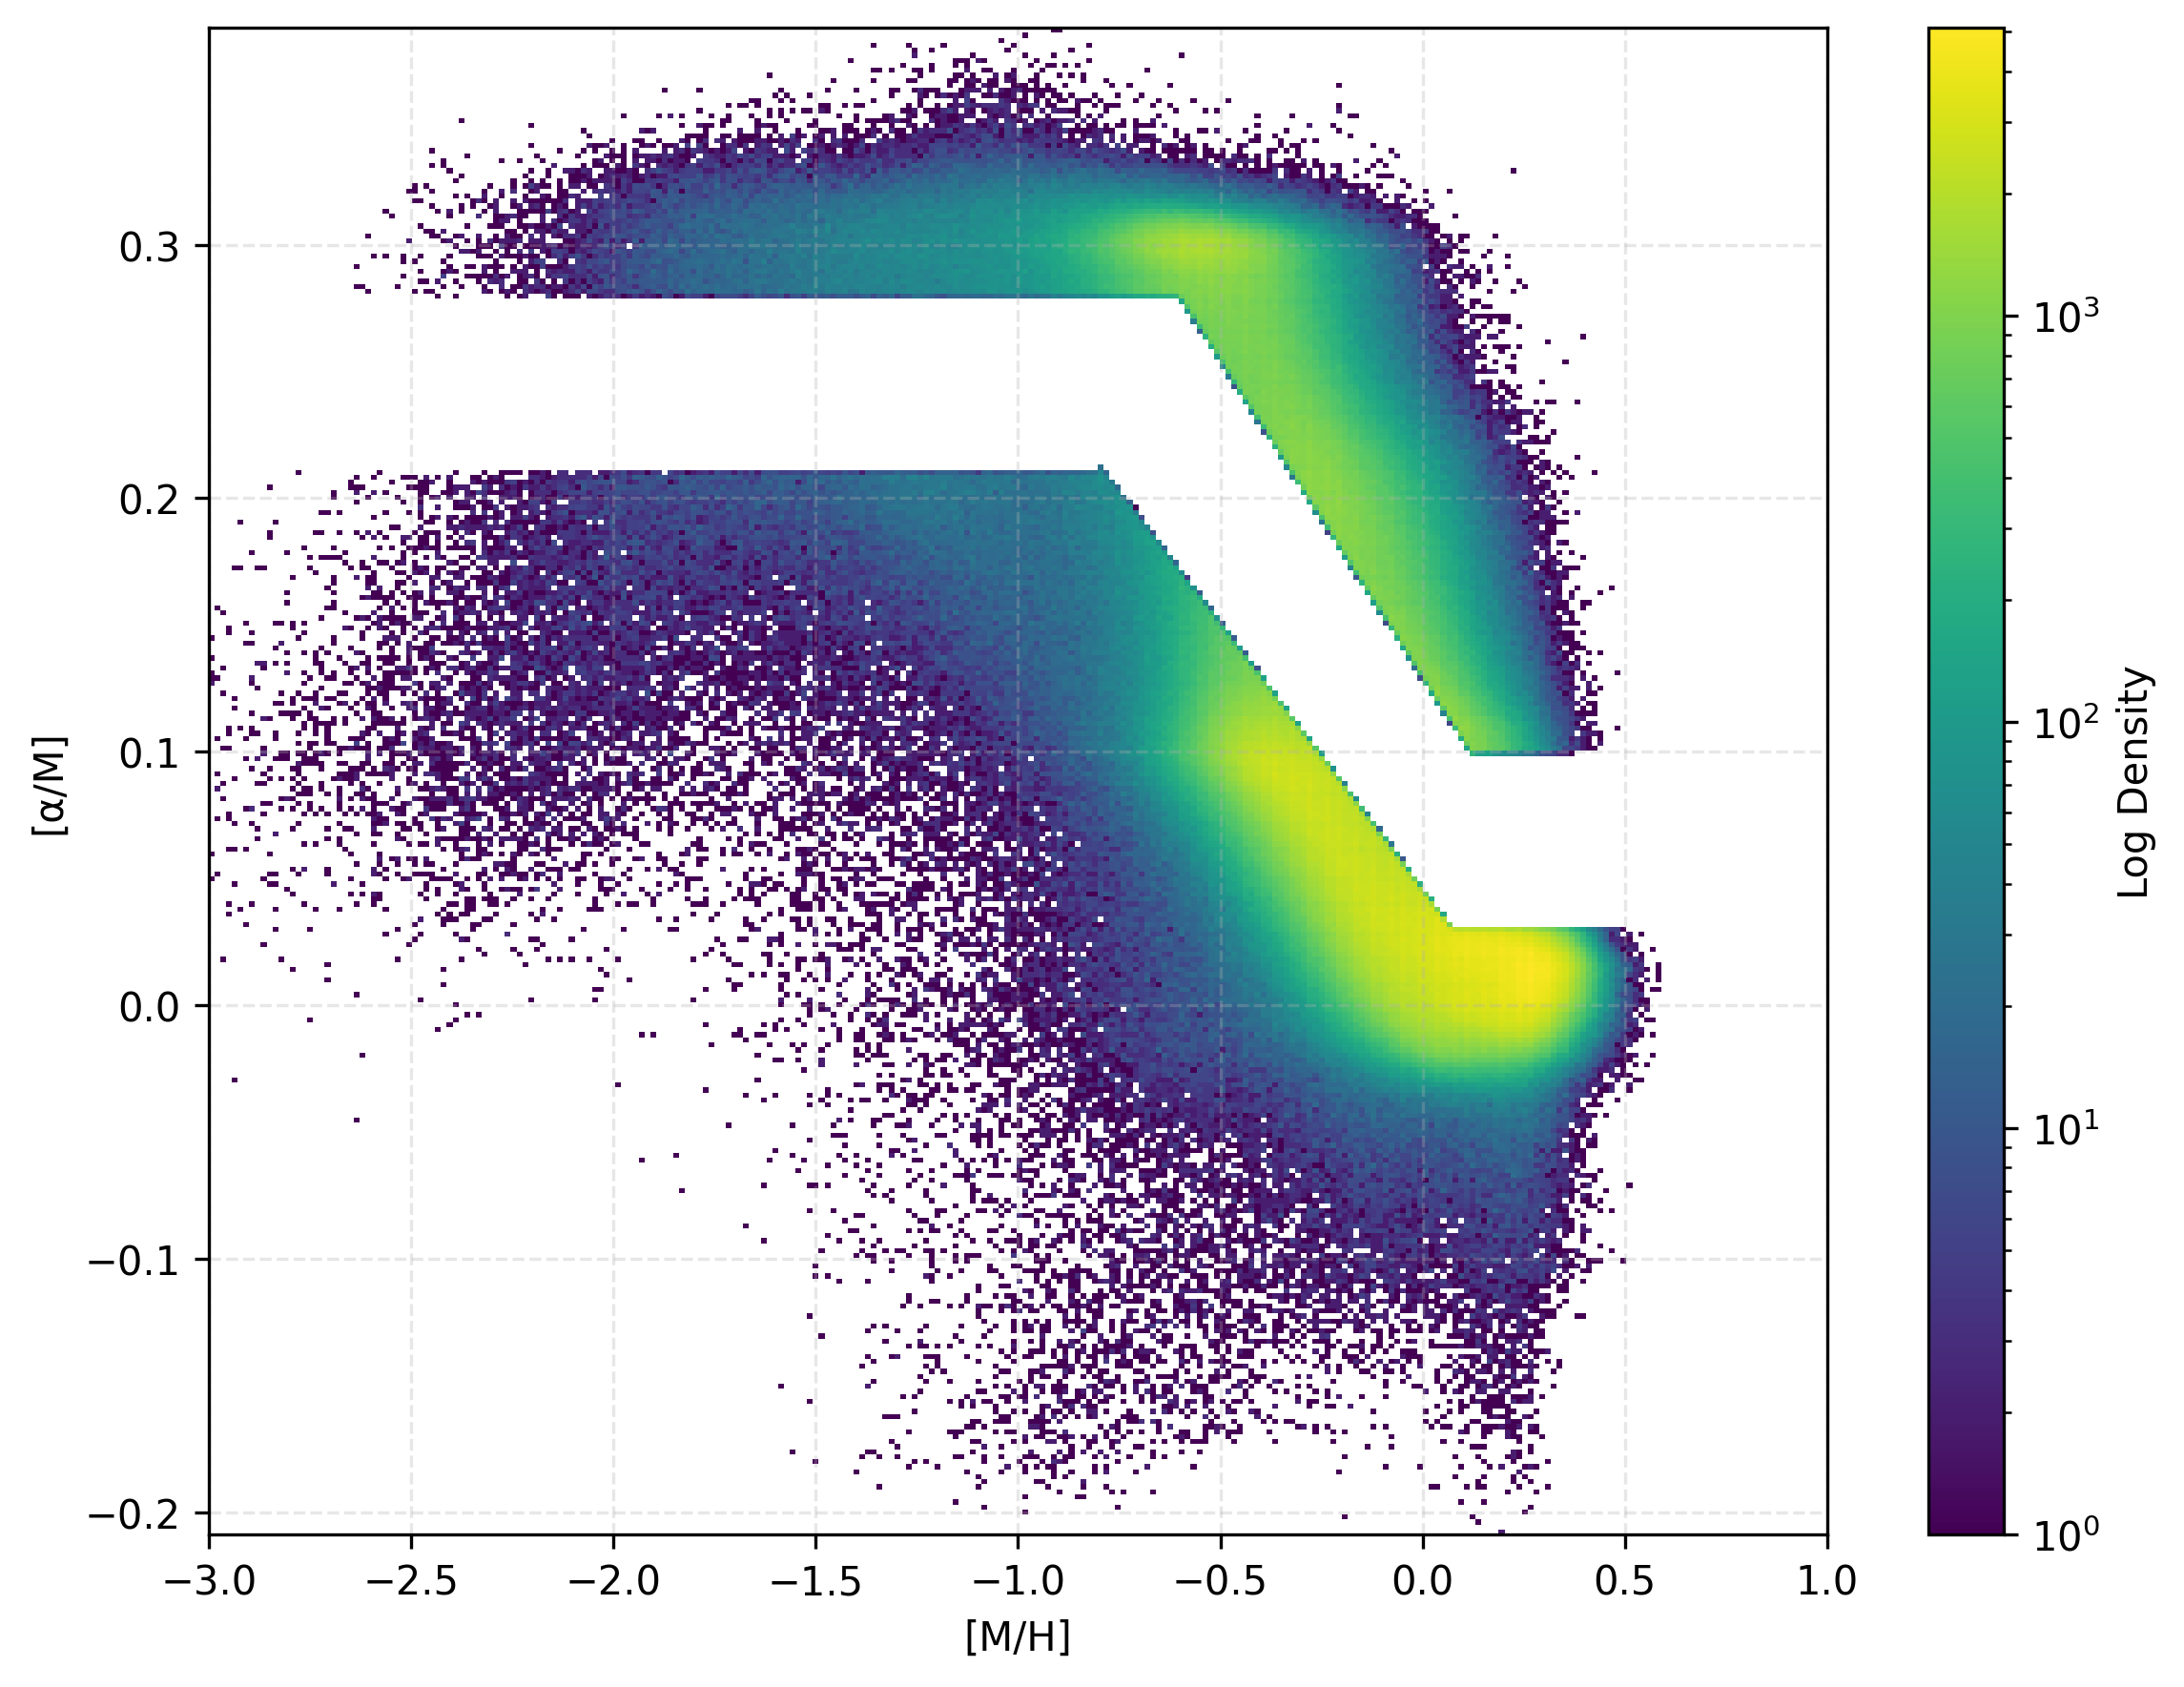
\includegraphics[width=0.49\textwidth]{../figures/alpha_vs_metalicity.png}
    \caption{Density of stars in the $[\alpha/\mathrm{M}]$–$[\mathrm{M/H}]$ plane.
             The high-$\alpha$ and low-$\alpha$ sequences are separated by the
             piece-wise linear boundary . The transition zone
             between the two sequences is clearly removed from this plot and discarded from
             subsequent analysis.}
    \label{fig:alphametal}
\end{figure}


  
Figure~\ref{fig:alphametal} displays the logarithmic density of our
RGB sample in the $[\alpha/\mathrm{M}]$–$[\mathrm{M/H}]$ plane.  Following
\citet{Chandra_2024}, but with a deliberately tighter boundary as in \citet{Vis2024}:

\[
\begin{aligned}
\text{high-}\alpha:\;&
  \begin{cases}
    [\mathrm{M/H}]<-0.60 &
      [\alpha/\mathrm{M}]>0.28\\
    -0.60\le[\mathrm{M/H}]\le0.125 &
      [\alpha/\mathrm{M}]>-0.25[\mathrm{M/H}]+0.13\\
    [\mathrm{M/H}]>0.125 &
      [\alpha/\mathrm{M}]>0.10
  \end{cases}\\[4pt]
\text{low-}\alpha:\;&
  \begin{cases}
    [\mathrm{M/H}]<-0.80 &
      [\alpha/\mathrm{M}]<0.21\\
    -0.80\le[\mathrm{M/H}]\le0.07 &
      [\alpha/\mathrm{M}]<-0.21[\mathrm{M/H}]+0.04
  \end{cases}
\end{aligned}
\]
%
and discard the intermediate “transition’’ band.

This high-$\alpha$ threshold is raised so that the
chemistry of the Gaia–Sausage/Enceladus debris
\citep{Belokurov2018,Helmi2018} does not leak into the
in-situ sequence;  
and the exclusion band is widened to maximise purity in both
sub-samples \citep{Vis2024}.  

Figure~\ref{fig:rz_metallicity} shows how metallicity varies with Galactocentric radius \(R\) and height \(z\).
The all-star map already hints at a global decline in \( [\mathrm{M/H}] \) away from the plane and the Solar circle.
This decline is more pronounced in the low-$\alpha$ sequence.


\begin{figure}[H]
  \centering
  \begin{subfigure}{0.6\textwidth}
    \centering
    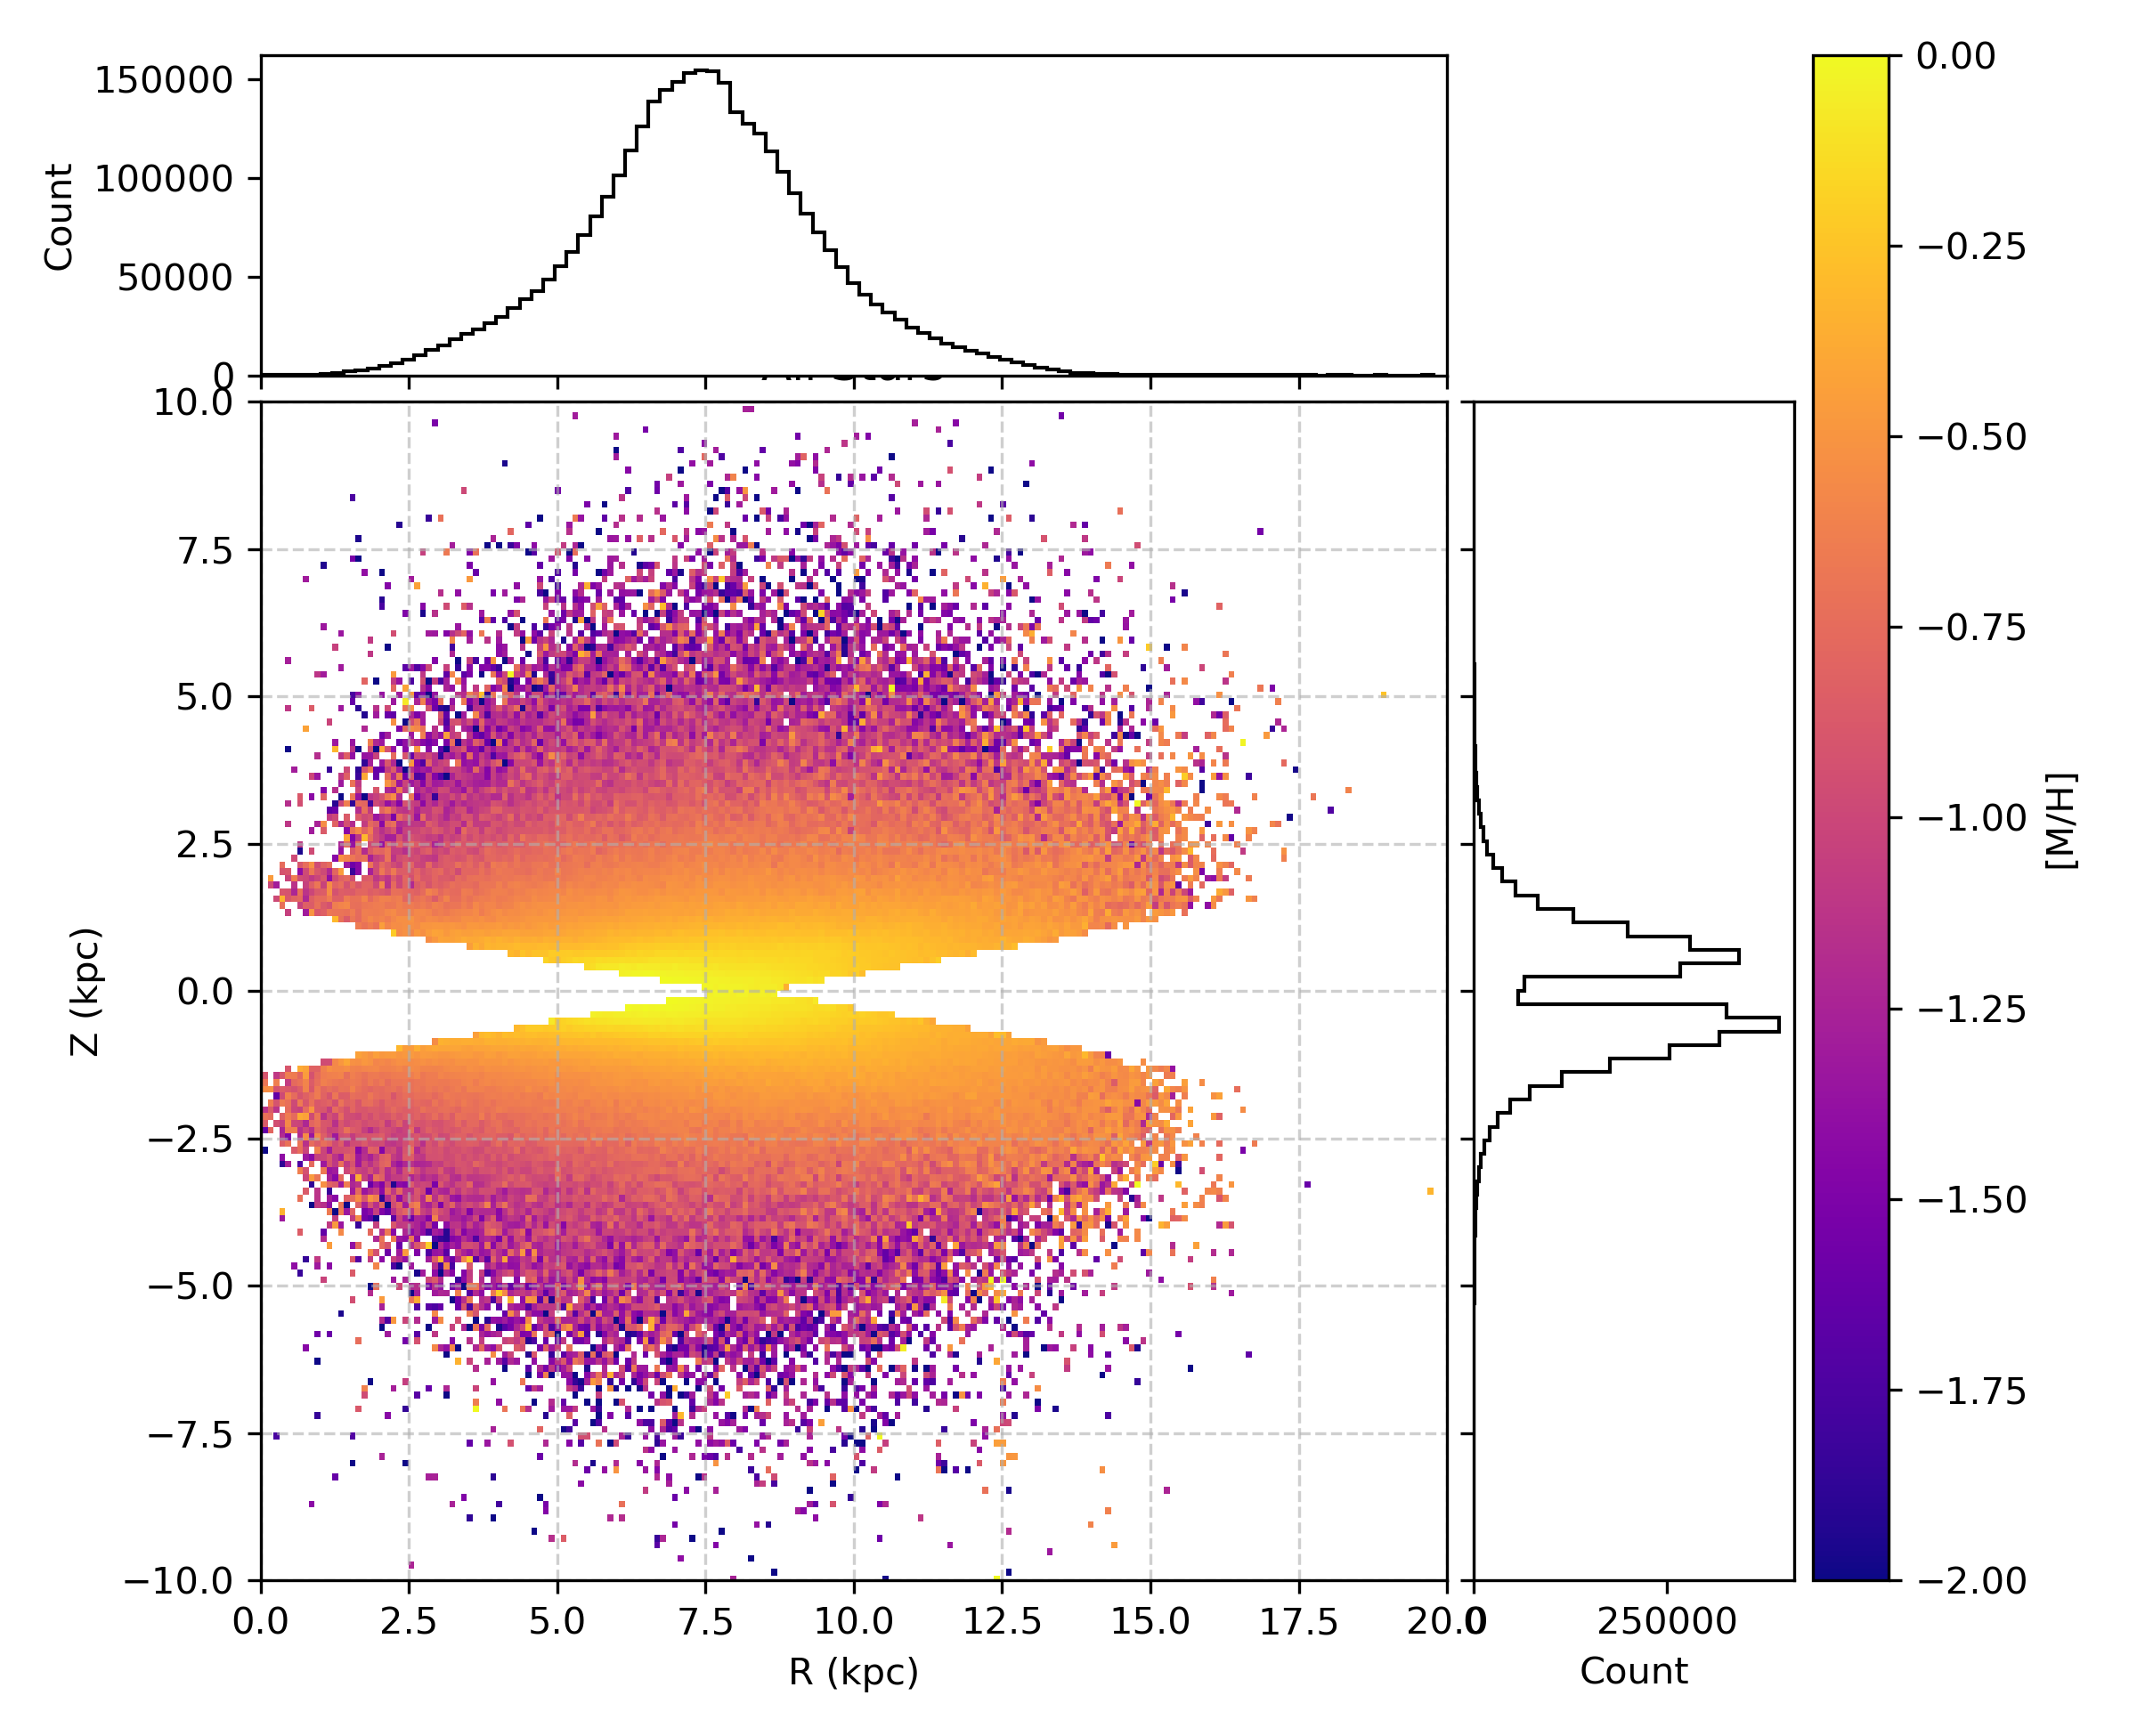
\includegraphics[width=\textwidth]{../figures/vis_rz_metallicity_all.png}
    \caption{All RGB stars}
    \label{fig:rz_all}
  \end{subfigure}

  \vspace{0.8em}

  \begin{subfigure}{0.45\textwidth}
    \centering
    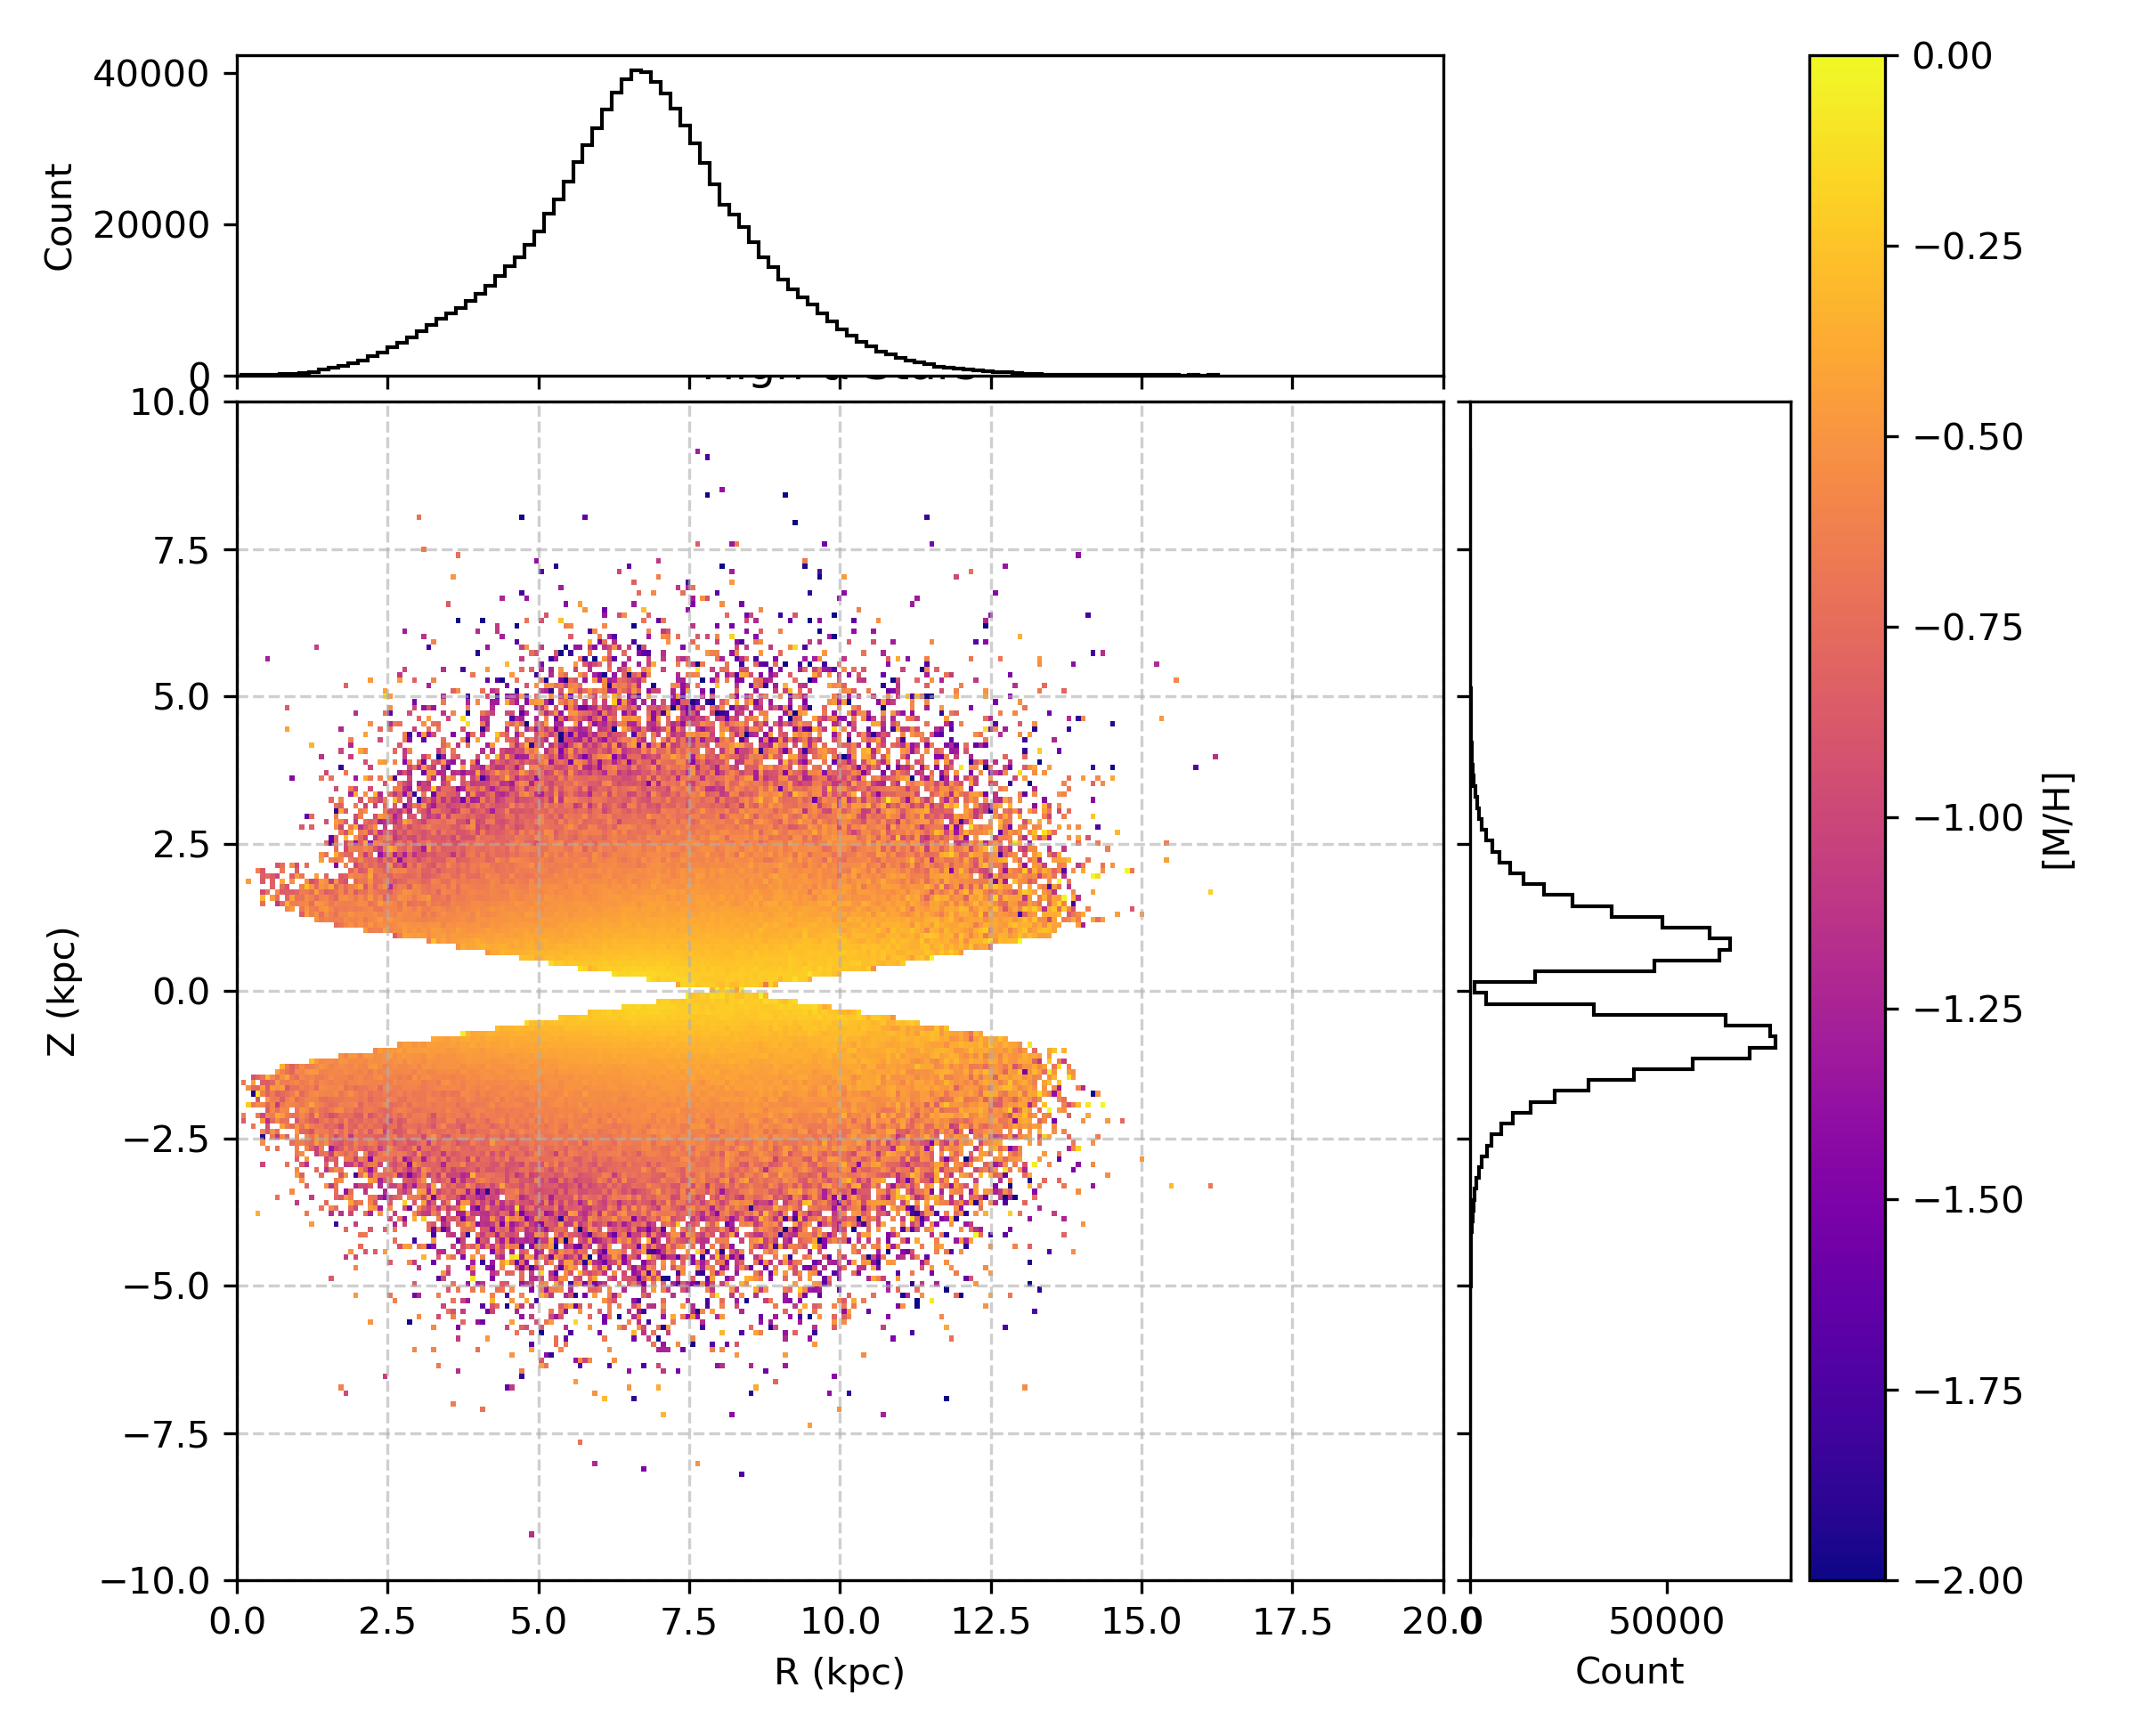
\includegraphics[width=\textwidth]{../figures/vis_rz_metallicity_high_alpha.png}
    \caption{High-$\alpha$ subsample}
    \label{fig:rz_highalpha}
  \end{subfigure}\hfill
  \begin{subfigure}{0.45\textwidth}
    \centering
    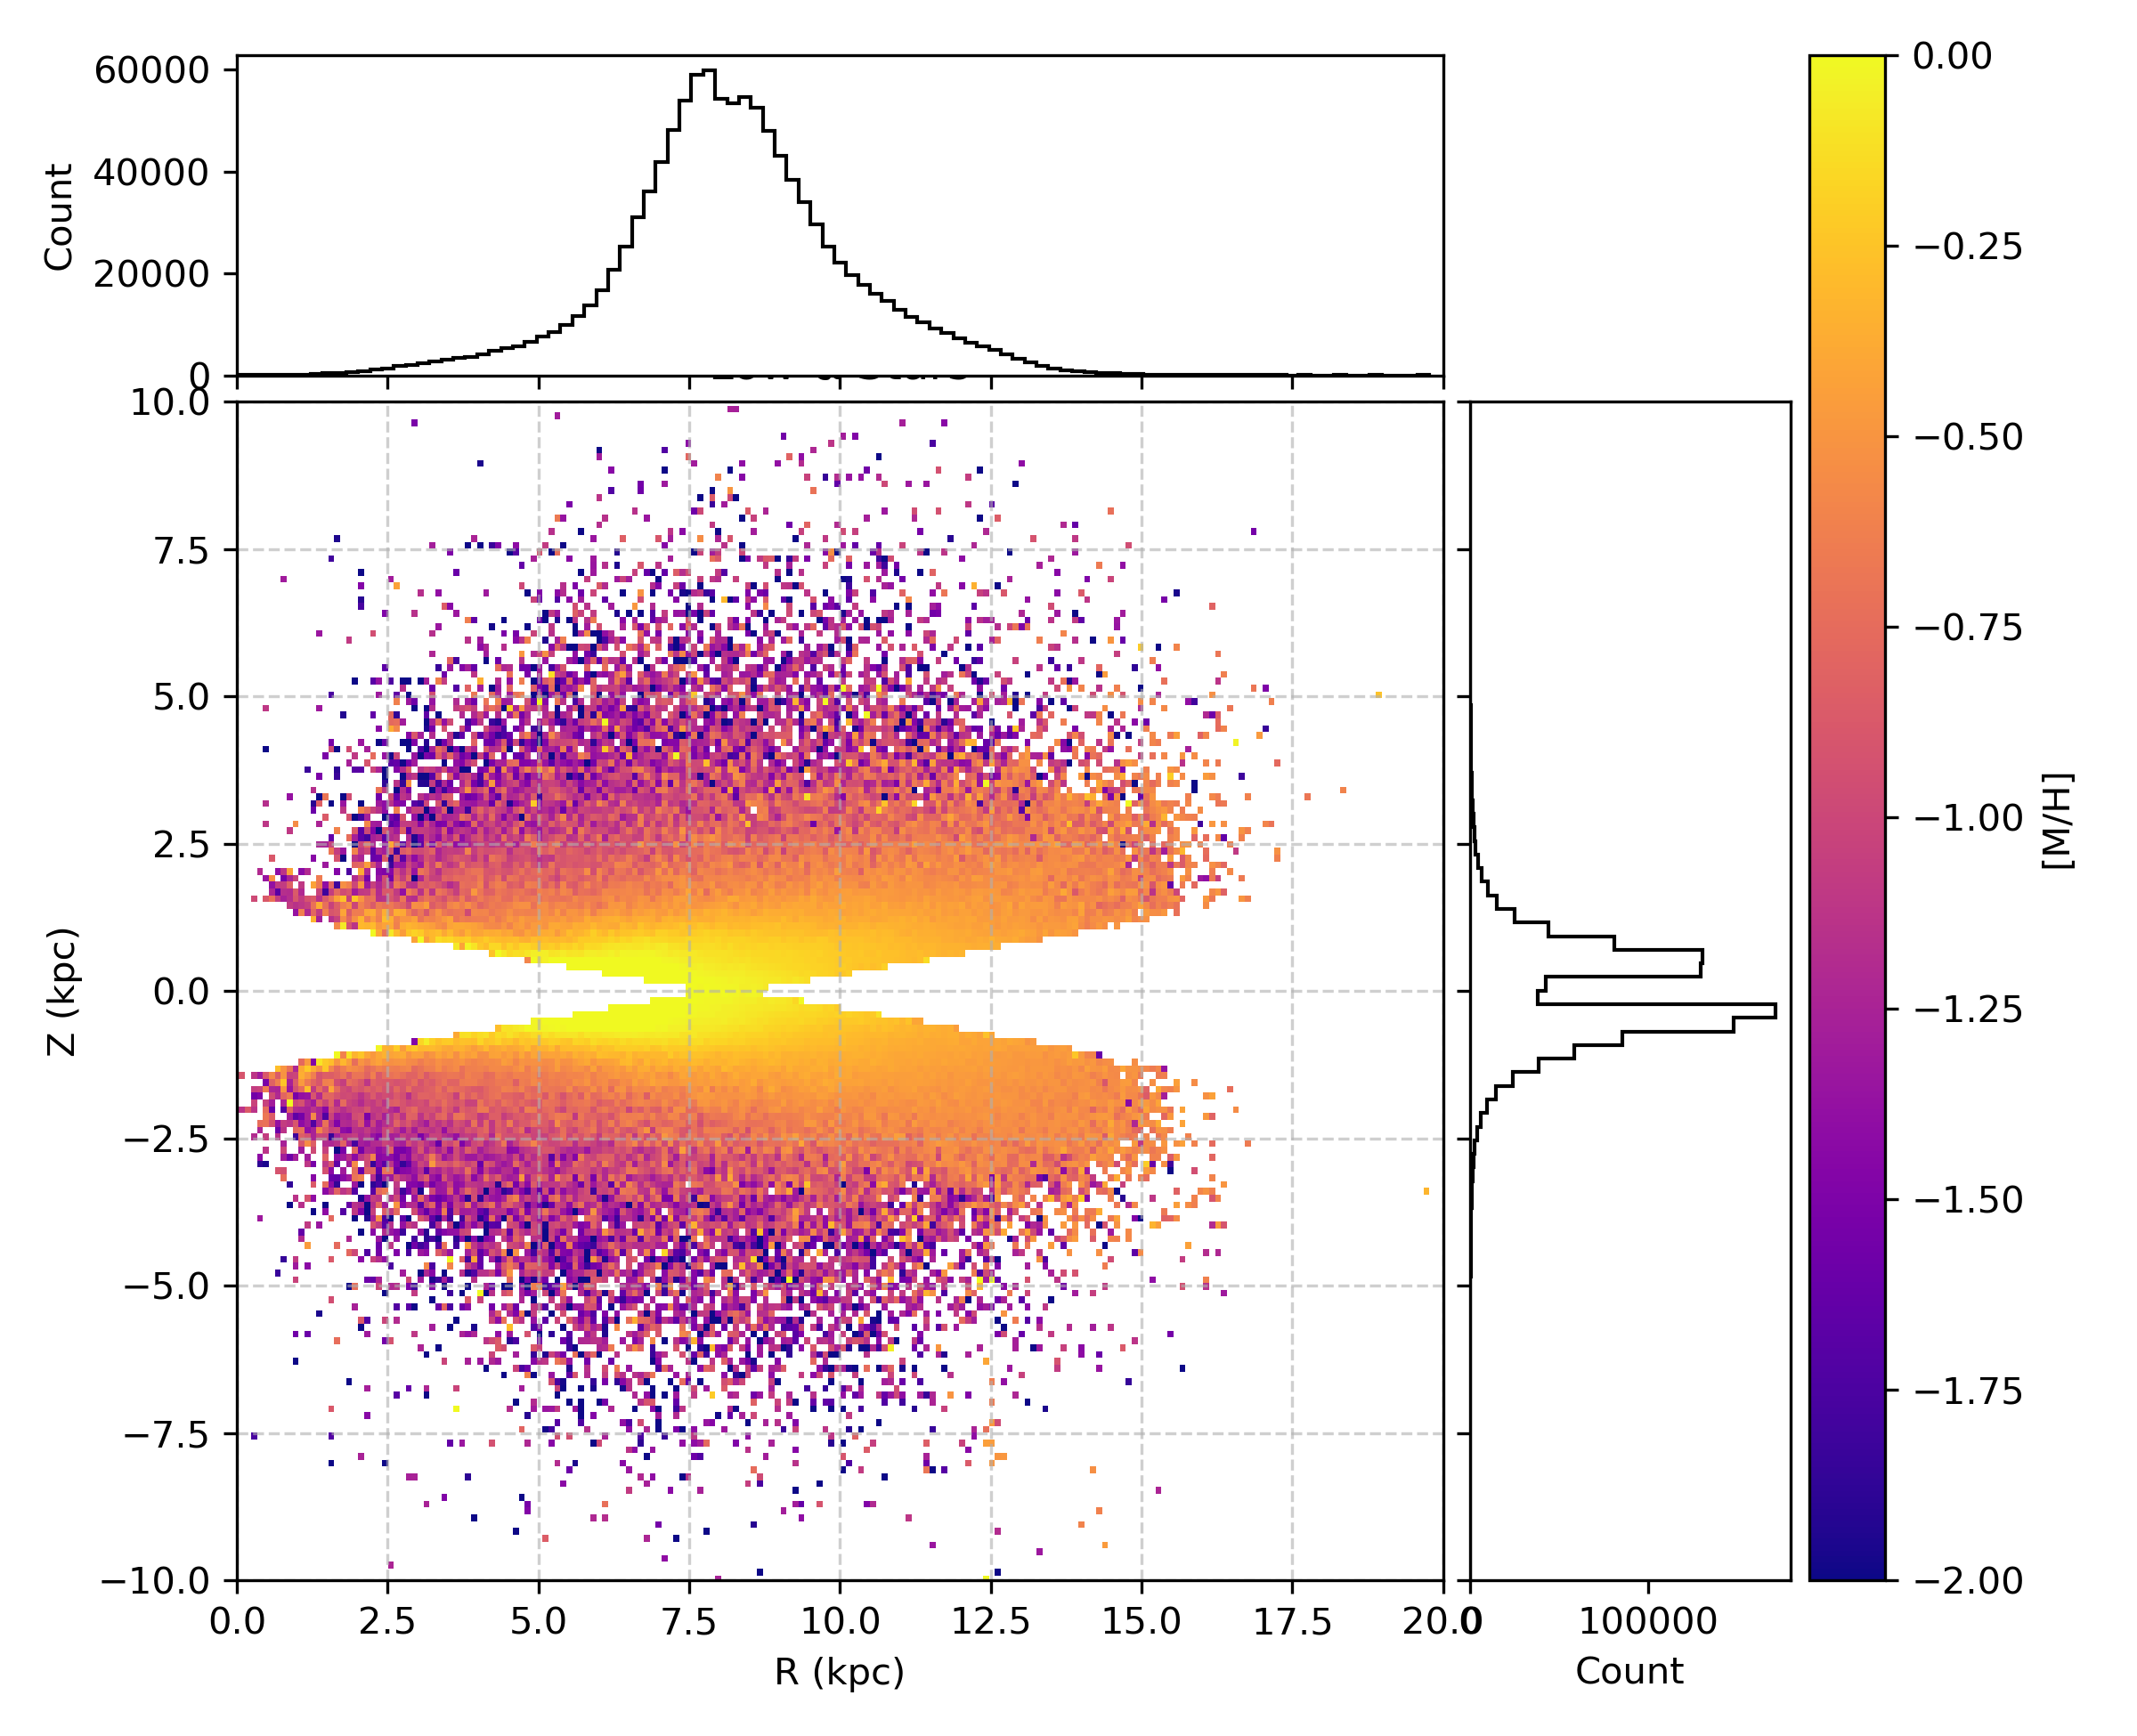
\includegraphics[width=\textwidth]{../figures/vis_rz_metallicity_low_alpha.png}
    \caption{Low-$\alpha$ subsample}
    \label{fig:rz_lowalpha}
  \end{subfigure}

  \caption{Mean $[\mathrm{M/H}]$ colour–coded in the
           Galactocentric $R$–$z$ plane.  
           \textit{Top:} the complete $G<16$ RGB sample.
           \textit{Bottom left:} high-$\alpha$ stars; \textit{bottom right:} low-$\alpha$ stars.
           The high-$\alpha$ population is more centrally concentrated and
           shows a shallower vertical metallicity gradient.}
  \label{fig:rz_metallicity}
\end{figure}

\begin{figure*}
  \centering
  %--------------------------- full sample --------------------------
  \begin{subfigure}[b]{0.32\textwidth}
    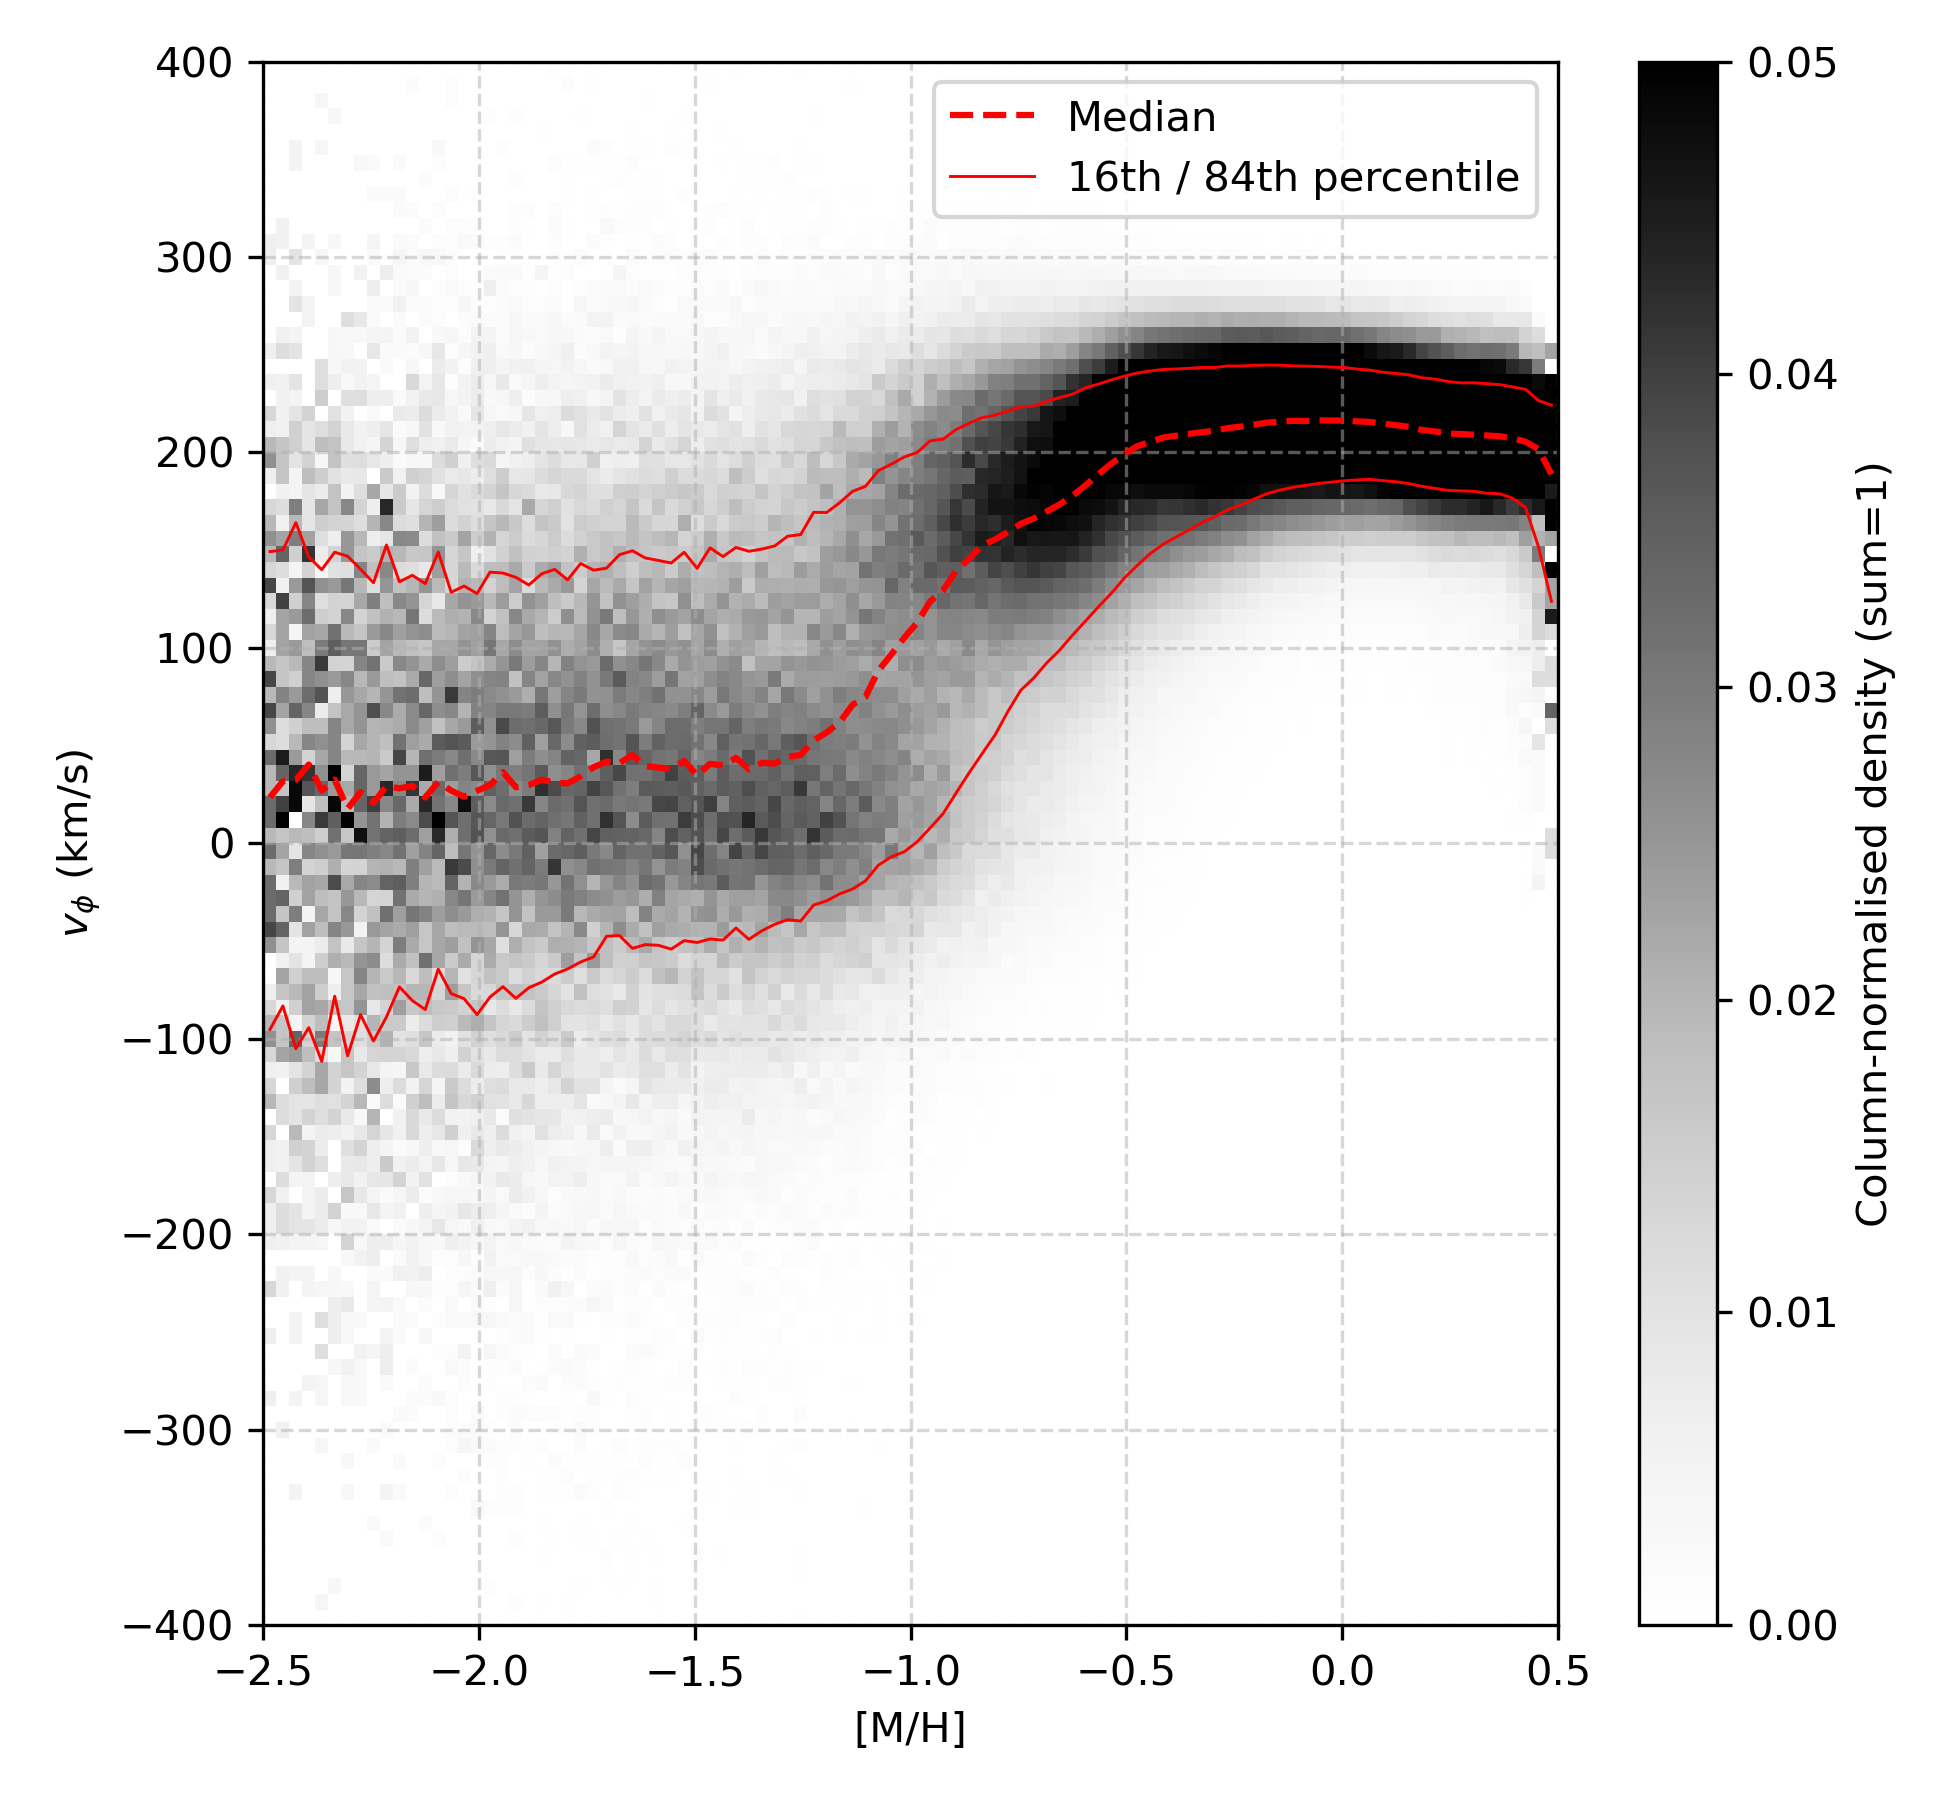
\includegraphics[width=\textwidth]{../figures/vis_mh_vphi_all.png}
    \caption{all RGB stars}
  \end{subfigure}\hfill
  %-------------------------- high-α sample --------------------------
  \begin{subfigure}[b]{0.32\textwidth}
    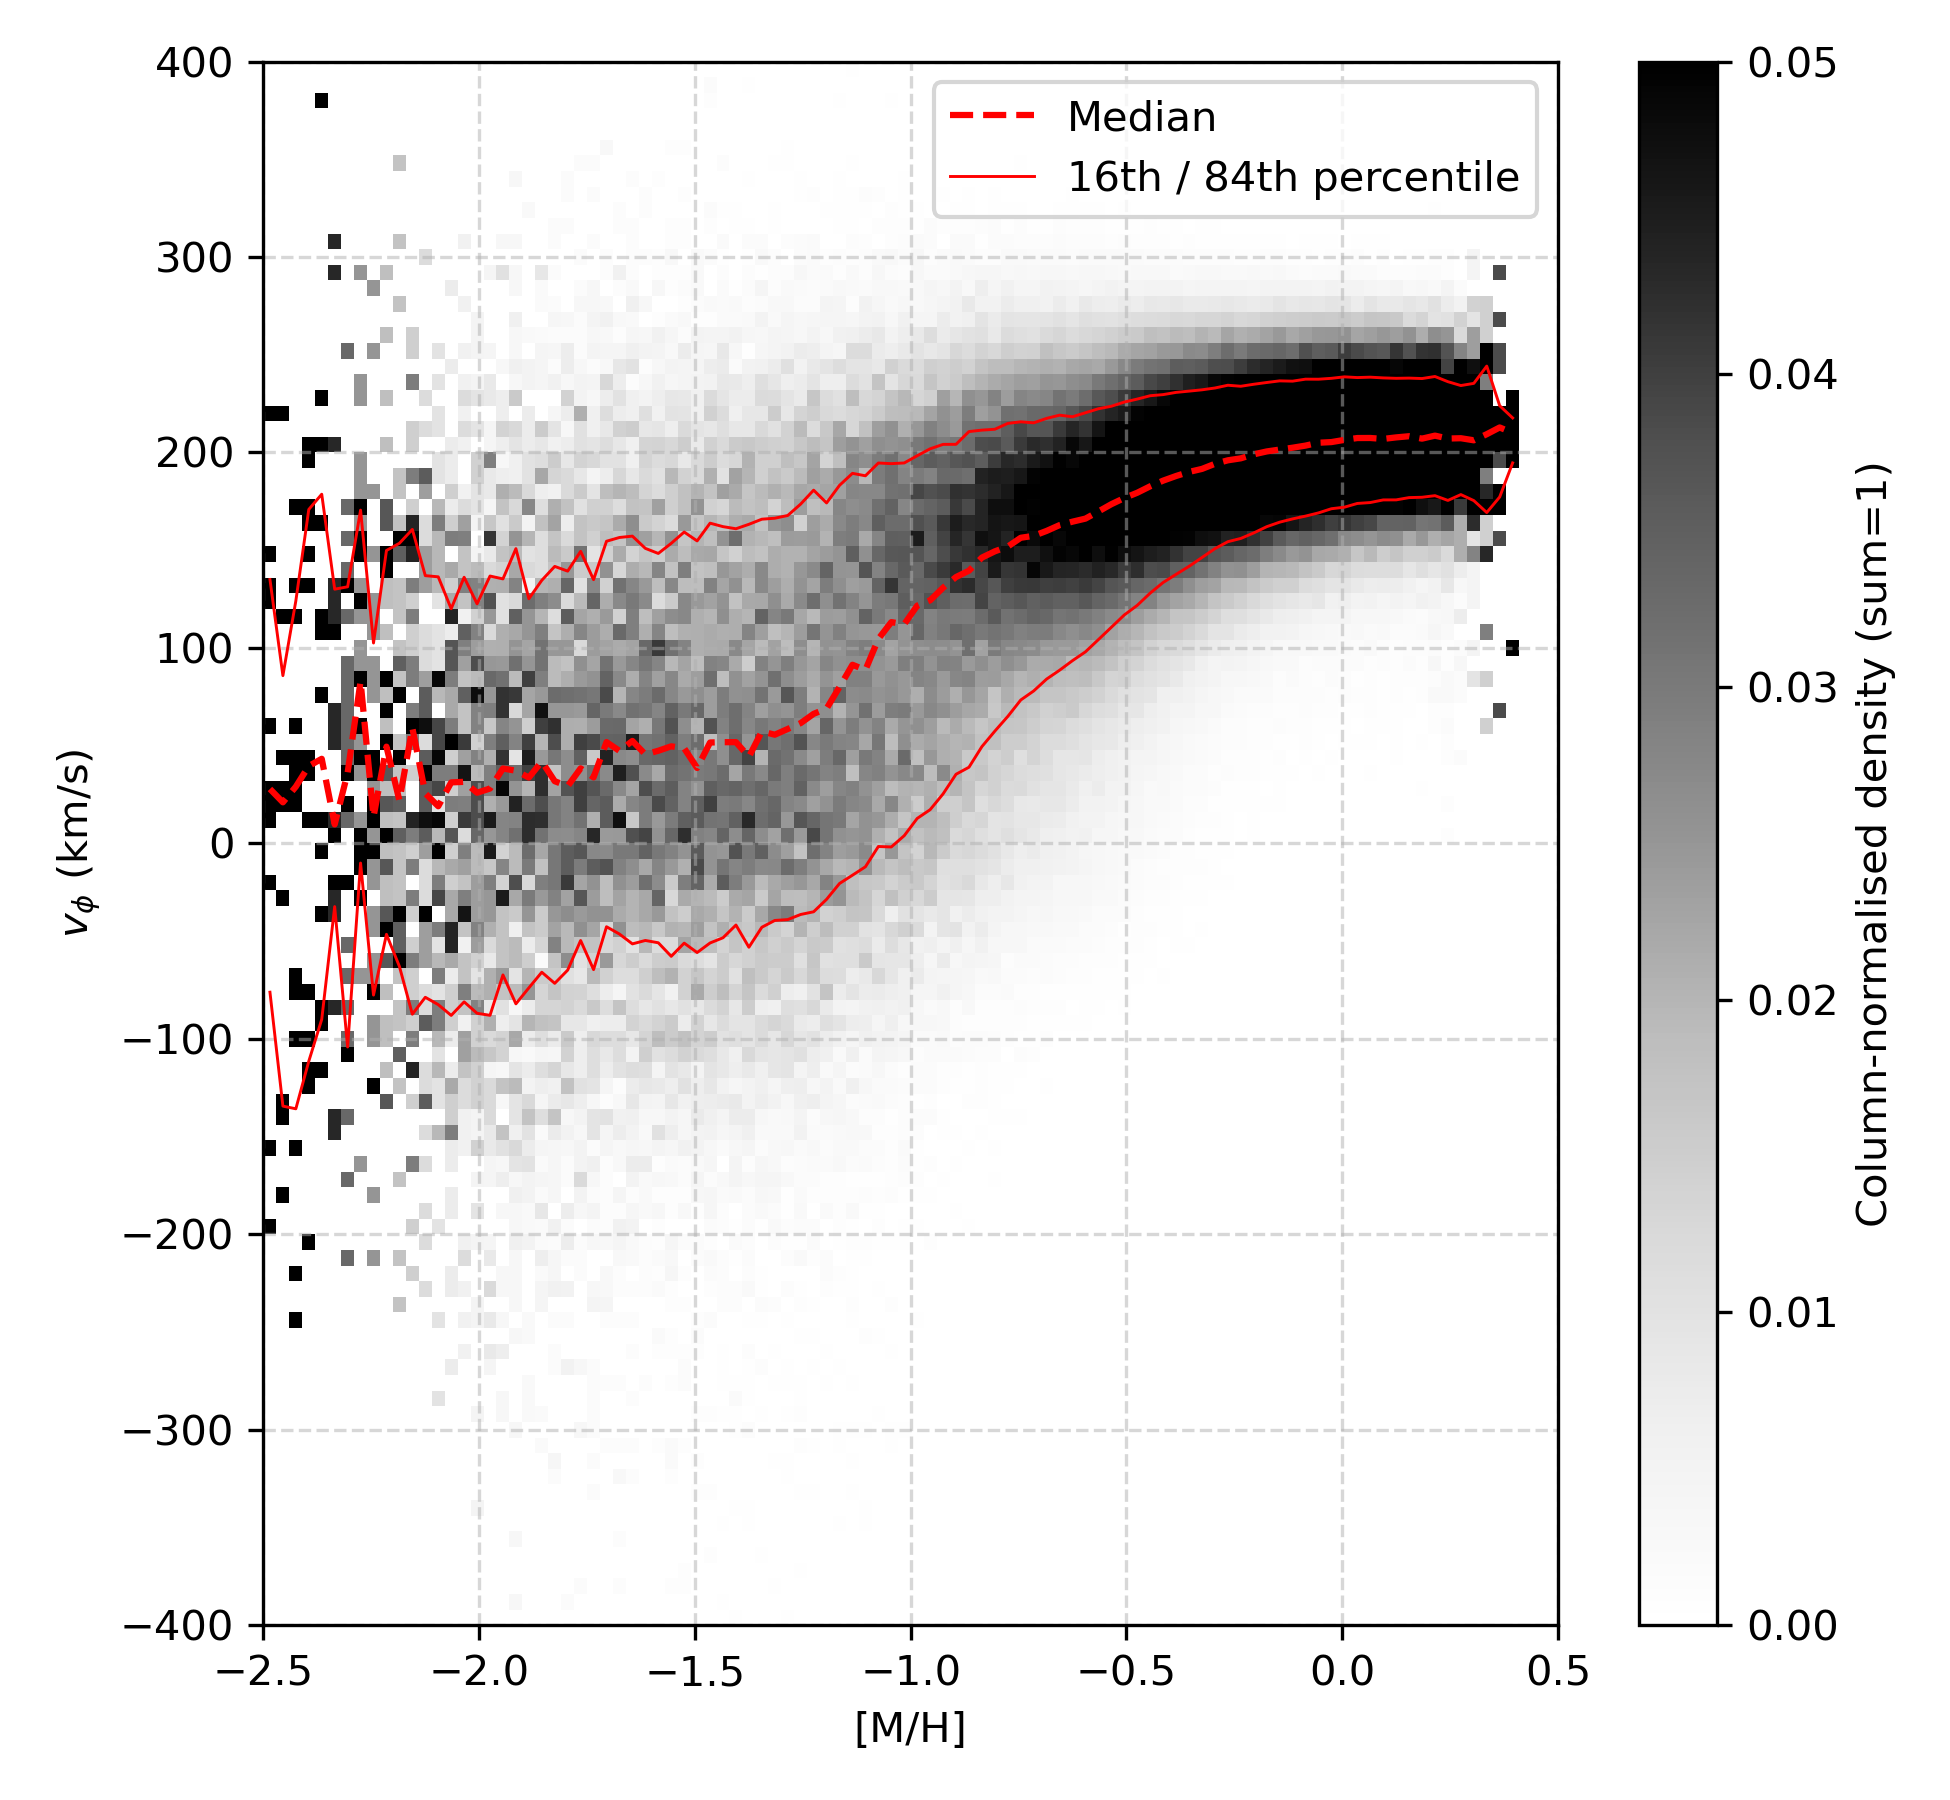
\includegraphics[width=\textwidth]{../figures/vis_mh_vphi_high_alpha.png}
    \caption{high-$\alpha$ sequence}
  \end{subfigure}\hfill
  %-------------------------- low-α sample ---------------------------
  \begin{subfigure}[b]{0.32\textwidth}
    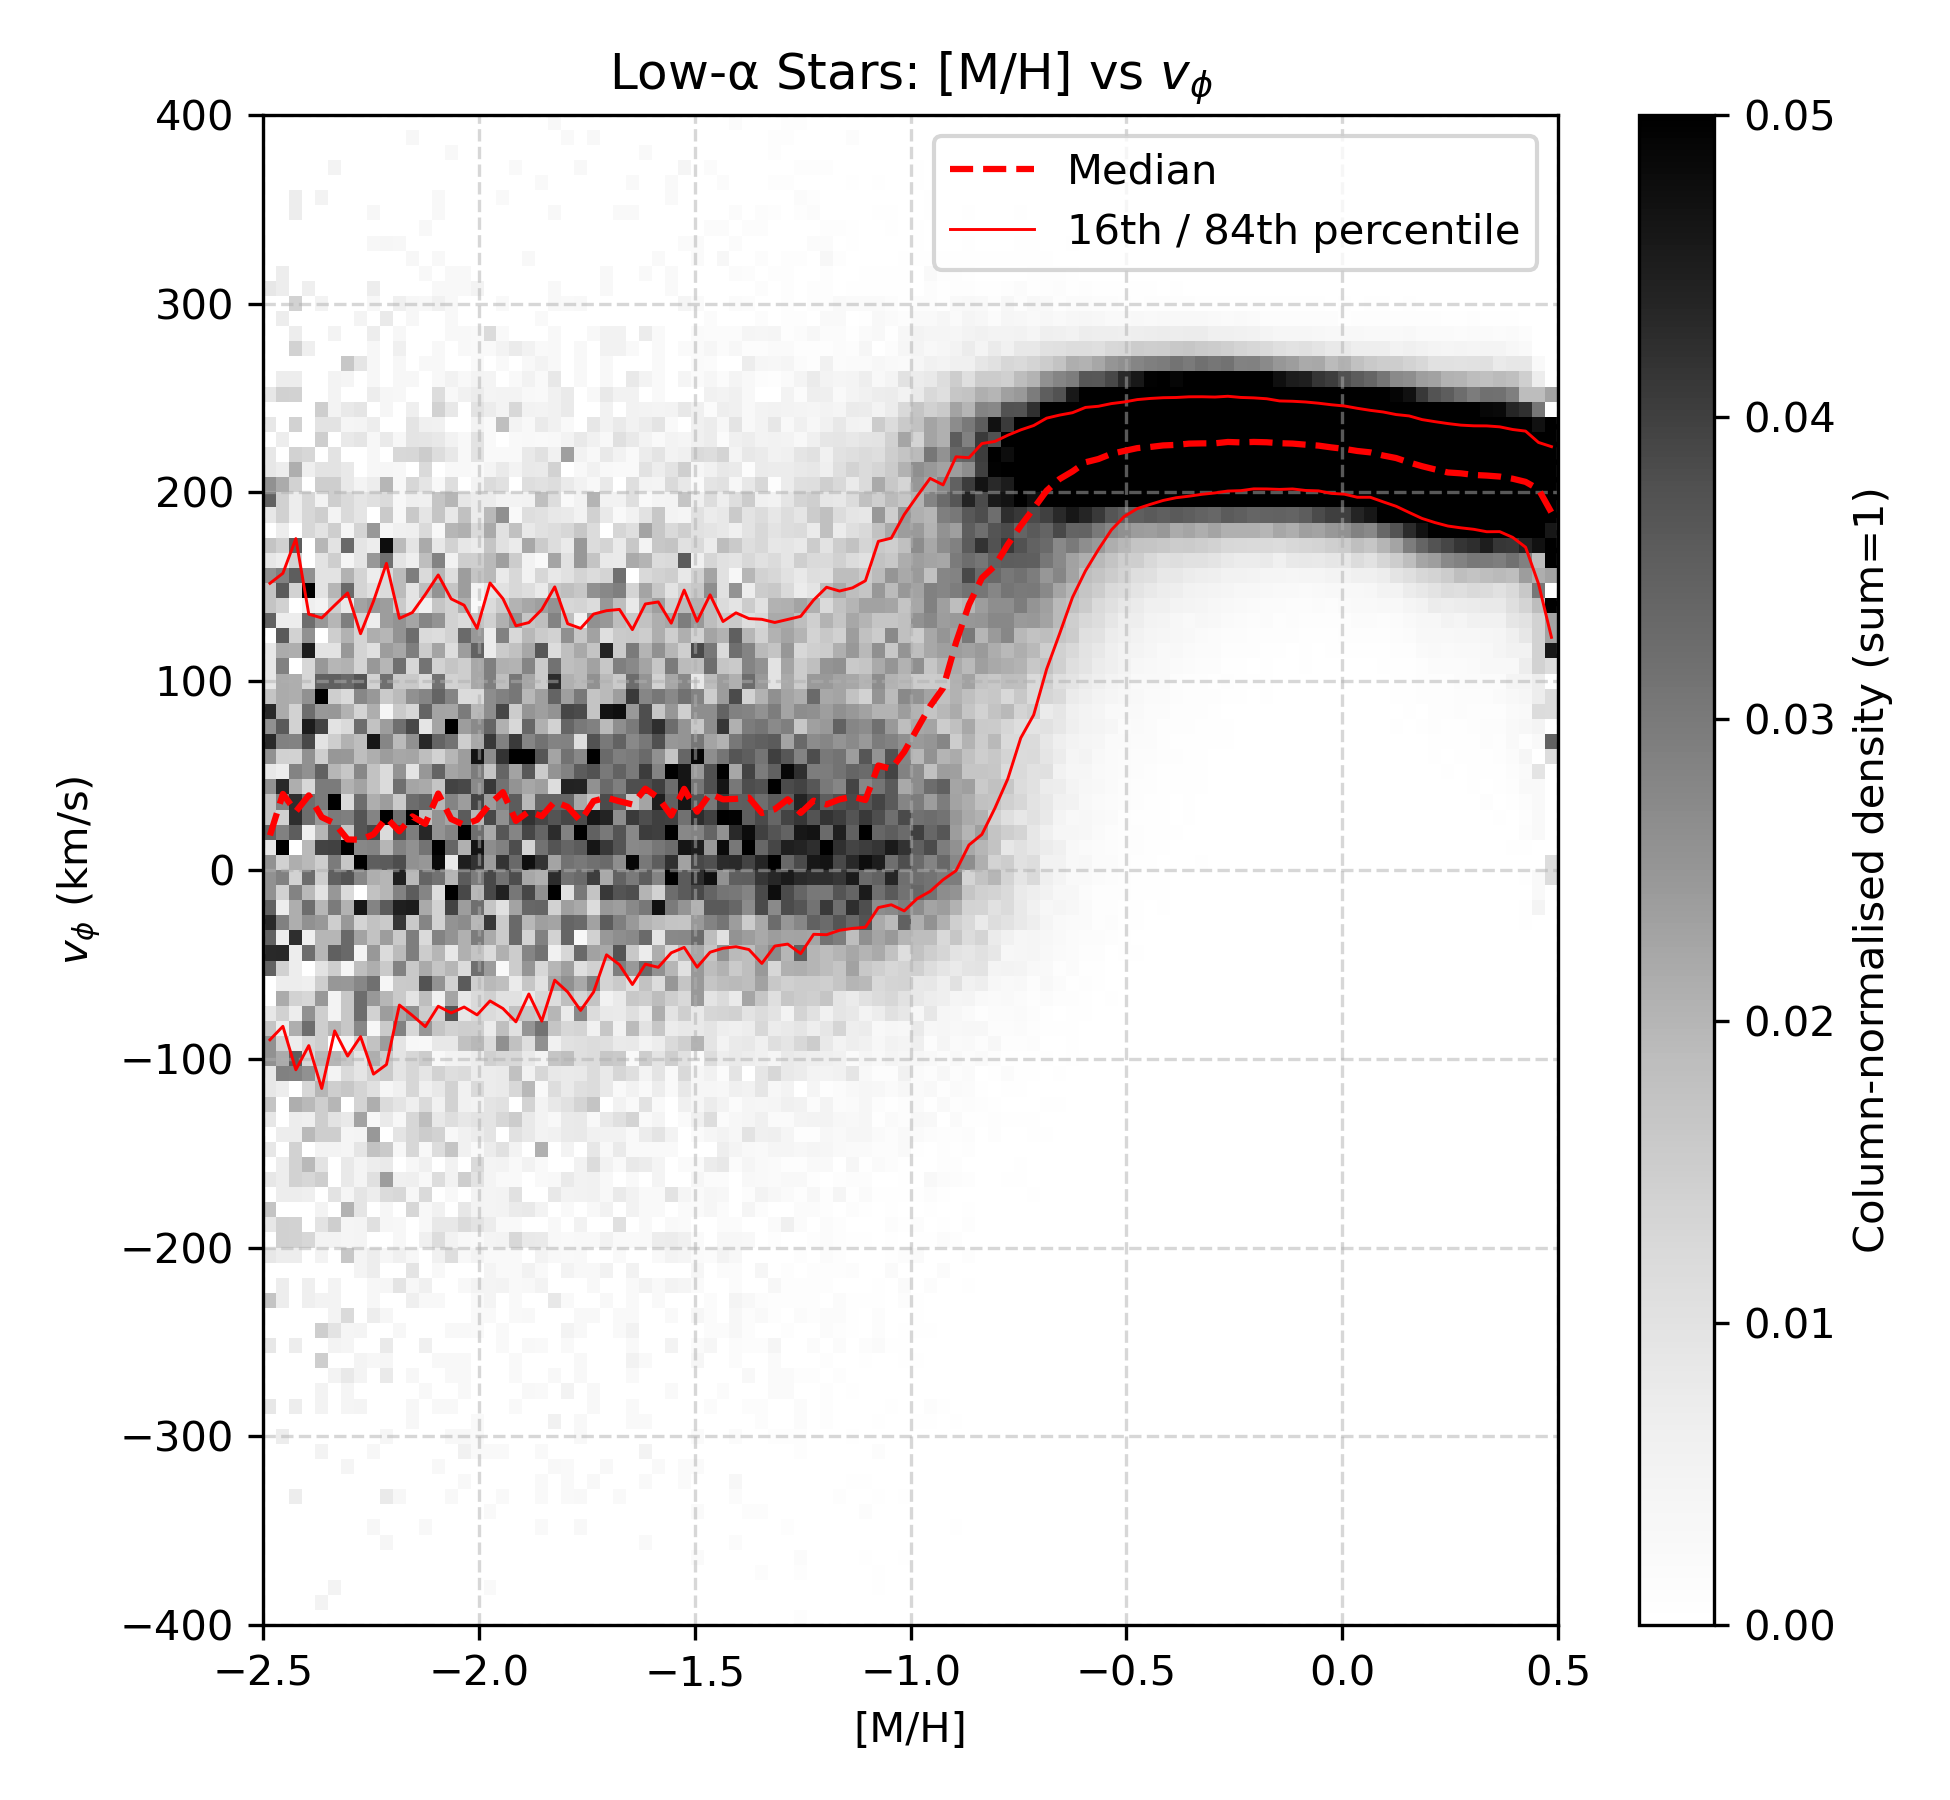
\includegraphics[width=\textwidth]{../figures/vis_mh_vphi_low_alpha.png}
    \caption{low-$\alpha$ sequence}
  \end{subfigure}

  \caption{Azimuthal velocity as a function of metallicity. 
           Each panel shows the column-normalised density in the
           $[\mathrm{M/H}]$–$v_\phi$ plane together with running medians
           (red dashed) and 16th/84th percentiles (black).  
           Left: full RGB sample.  Centre / right: chemically separated
           high-$\alpha$ and low-$\alpha$ subsamples defined in
           Sect.~\ref{sec:data}.}
  \label{fig:mh_vphi_alpha}
\end{figure*}

 

As shown in Figure~\ref{fig:mh_vphi_alpha}, high-$\alpha$ giants 
exhibit a gradual spin-up with increasing metallicity.  
At low metallicities ($[\mathrm{M/H}]\lesssim -2$), the population 
shows mild net prograde rotation with large dispersion, 
consistent with a dynamically hot stellar halo. From $[\mathrm{M/H}]\gtrsim -1.3$, 
there is a steady increase in rotation velocity and a corresponding decrease in 
dispersion, indicative of a transition toward the thick disc.  
By $[\mathrm{M/H}]\gtrsim -0.5$, most stars occupy a kinematic regime characterised 
by elevated $v_\phi$ and moderate dispersion, consistent with a dynamically hot 
but rotationally supported thick disc. This continuous trend supports 
a scenario in which the Galaxy’s in-situ population gradually acquired angular 
momentum as star formation progressed.


In the low-$\alpha$ panel, stars with $[\mathrm{M/H}]\lesssim -1.2$ exhibit kinematics similar 
to those in the high-$\alpha$ sequence, showing mild prograde rotation and high velocity dispersion. 
However, above $[\mathrm{M/H}]\gtrsim -1.2$, the low-$\alpha$ sequence 
undergoes a sharper transition to a population with high net prograde rotation and lower velocity dispersion. 
By $[\mathrm{M/H}]\gtrsim -0.5$, the low-$\alpha$ population exhibits kinematics consistent with the thin disc: 
a strongly rotating, dynamically cold component with lower dispersion than the high-$\alpha$ sequence.


In summary, the high-$\alpha$ sequence shows a gradual transition from
a dynamically hot halo to a thick disc, while the low-$\alpha$ sequence
shows a more abrupt transition to a dynamically cold disc at higher metallicities.



Following the method described in Section~\ref{subsec:velocities}, we obtain full six-dimensional
phase-space coordinates for the chemically separated high- and low-$\alpha$ subsamples.
Figure~\ref{fig:vr_vphi_alpha} shows the distribution of stars in the $v_R$–$v_\phi$ plane
across metallicity bins for the high-$\alpha$ (top) and low-$\alpha$ (bottom) populations.

The low-$\alpha$ sample exhibits a strong rotationally supported component, particularly at
higher metallicities ($[\mathrm{M/H}] \gtrsim -1.0$), with a narrow $v_\phi$ distribution centred
around $\sim200$ km/s and low radial velocity dispersion—clear hallmarks of thin-disc kinematics.
As metallicity decreases, this rotational component becomes less pronounced, with broader
distributions in both $v_R$ and $v_\phi$ appearing at $[\mathrm{M/H}] \lesssim -1.5$, consistent
with increased contamination from halo or accreted populations.

The high-$\alpha$ stars, by contrast, show a continuous transition from a kinematically hot,
low-rotation regime at low metallicities to a more rotation-supported disc at higher
metallicities. This reflects the gradual build-up of the thick disc over time, as also noted in
\citet{Chandra_2024}. The velocity dispersion is broader throughout,
indicating that high-$\alpha$ stars trace older, more dynamically heated populations.

\begin{figure}[H]
  \centering
  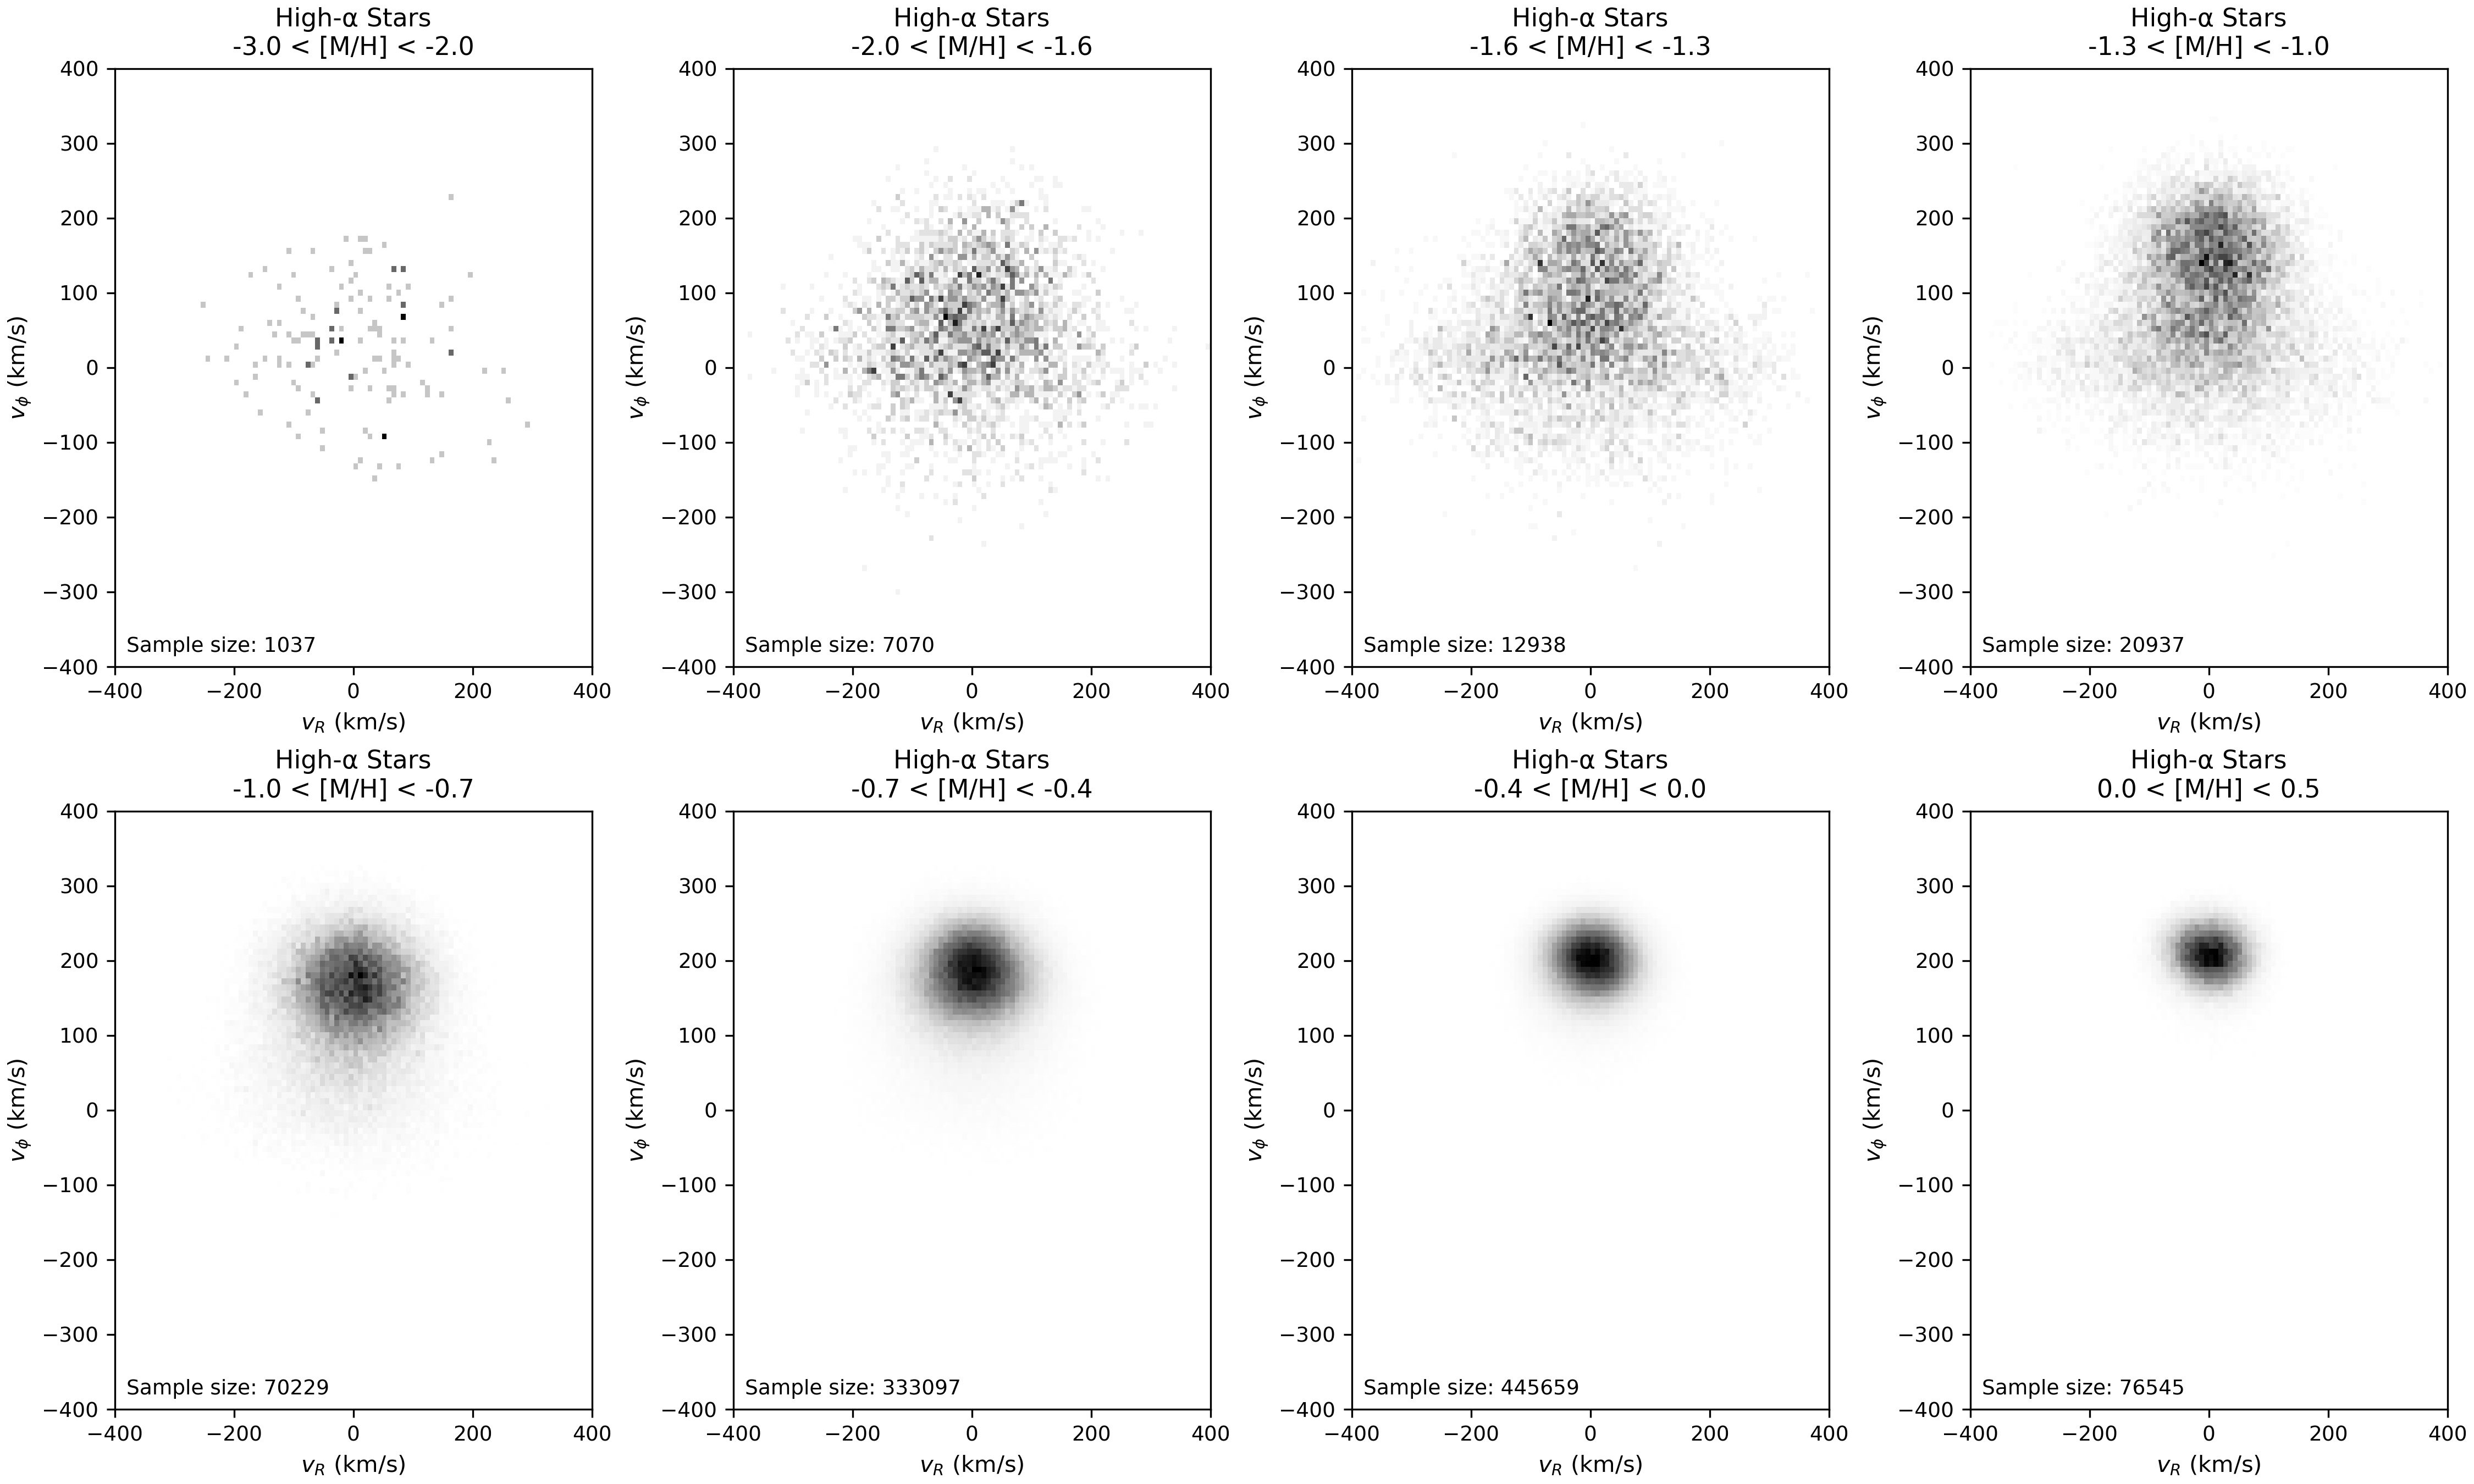
\includegraphics[width=\textwidth]{../figures/high_alpha.png}
  \vspace{0.5em}
  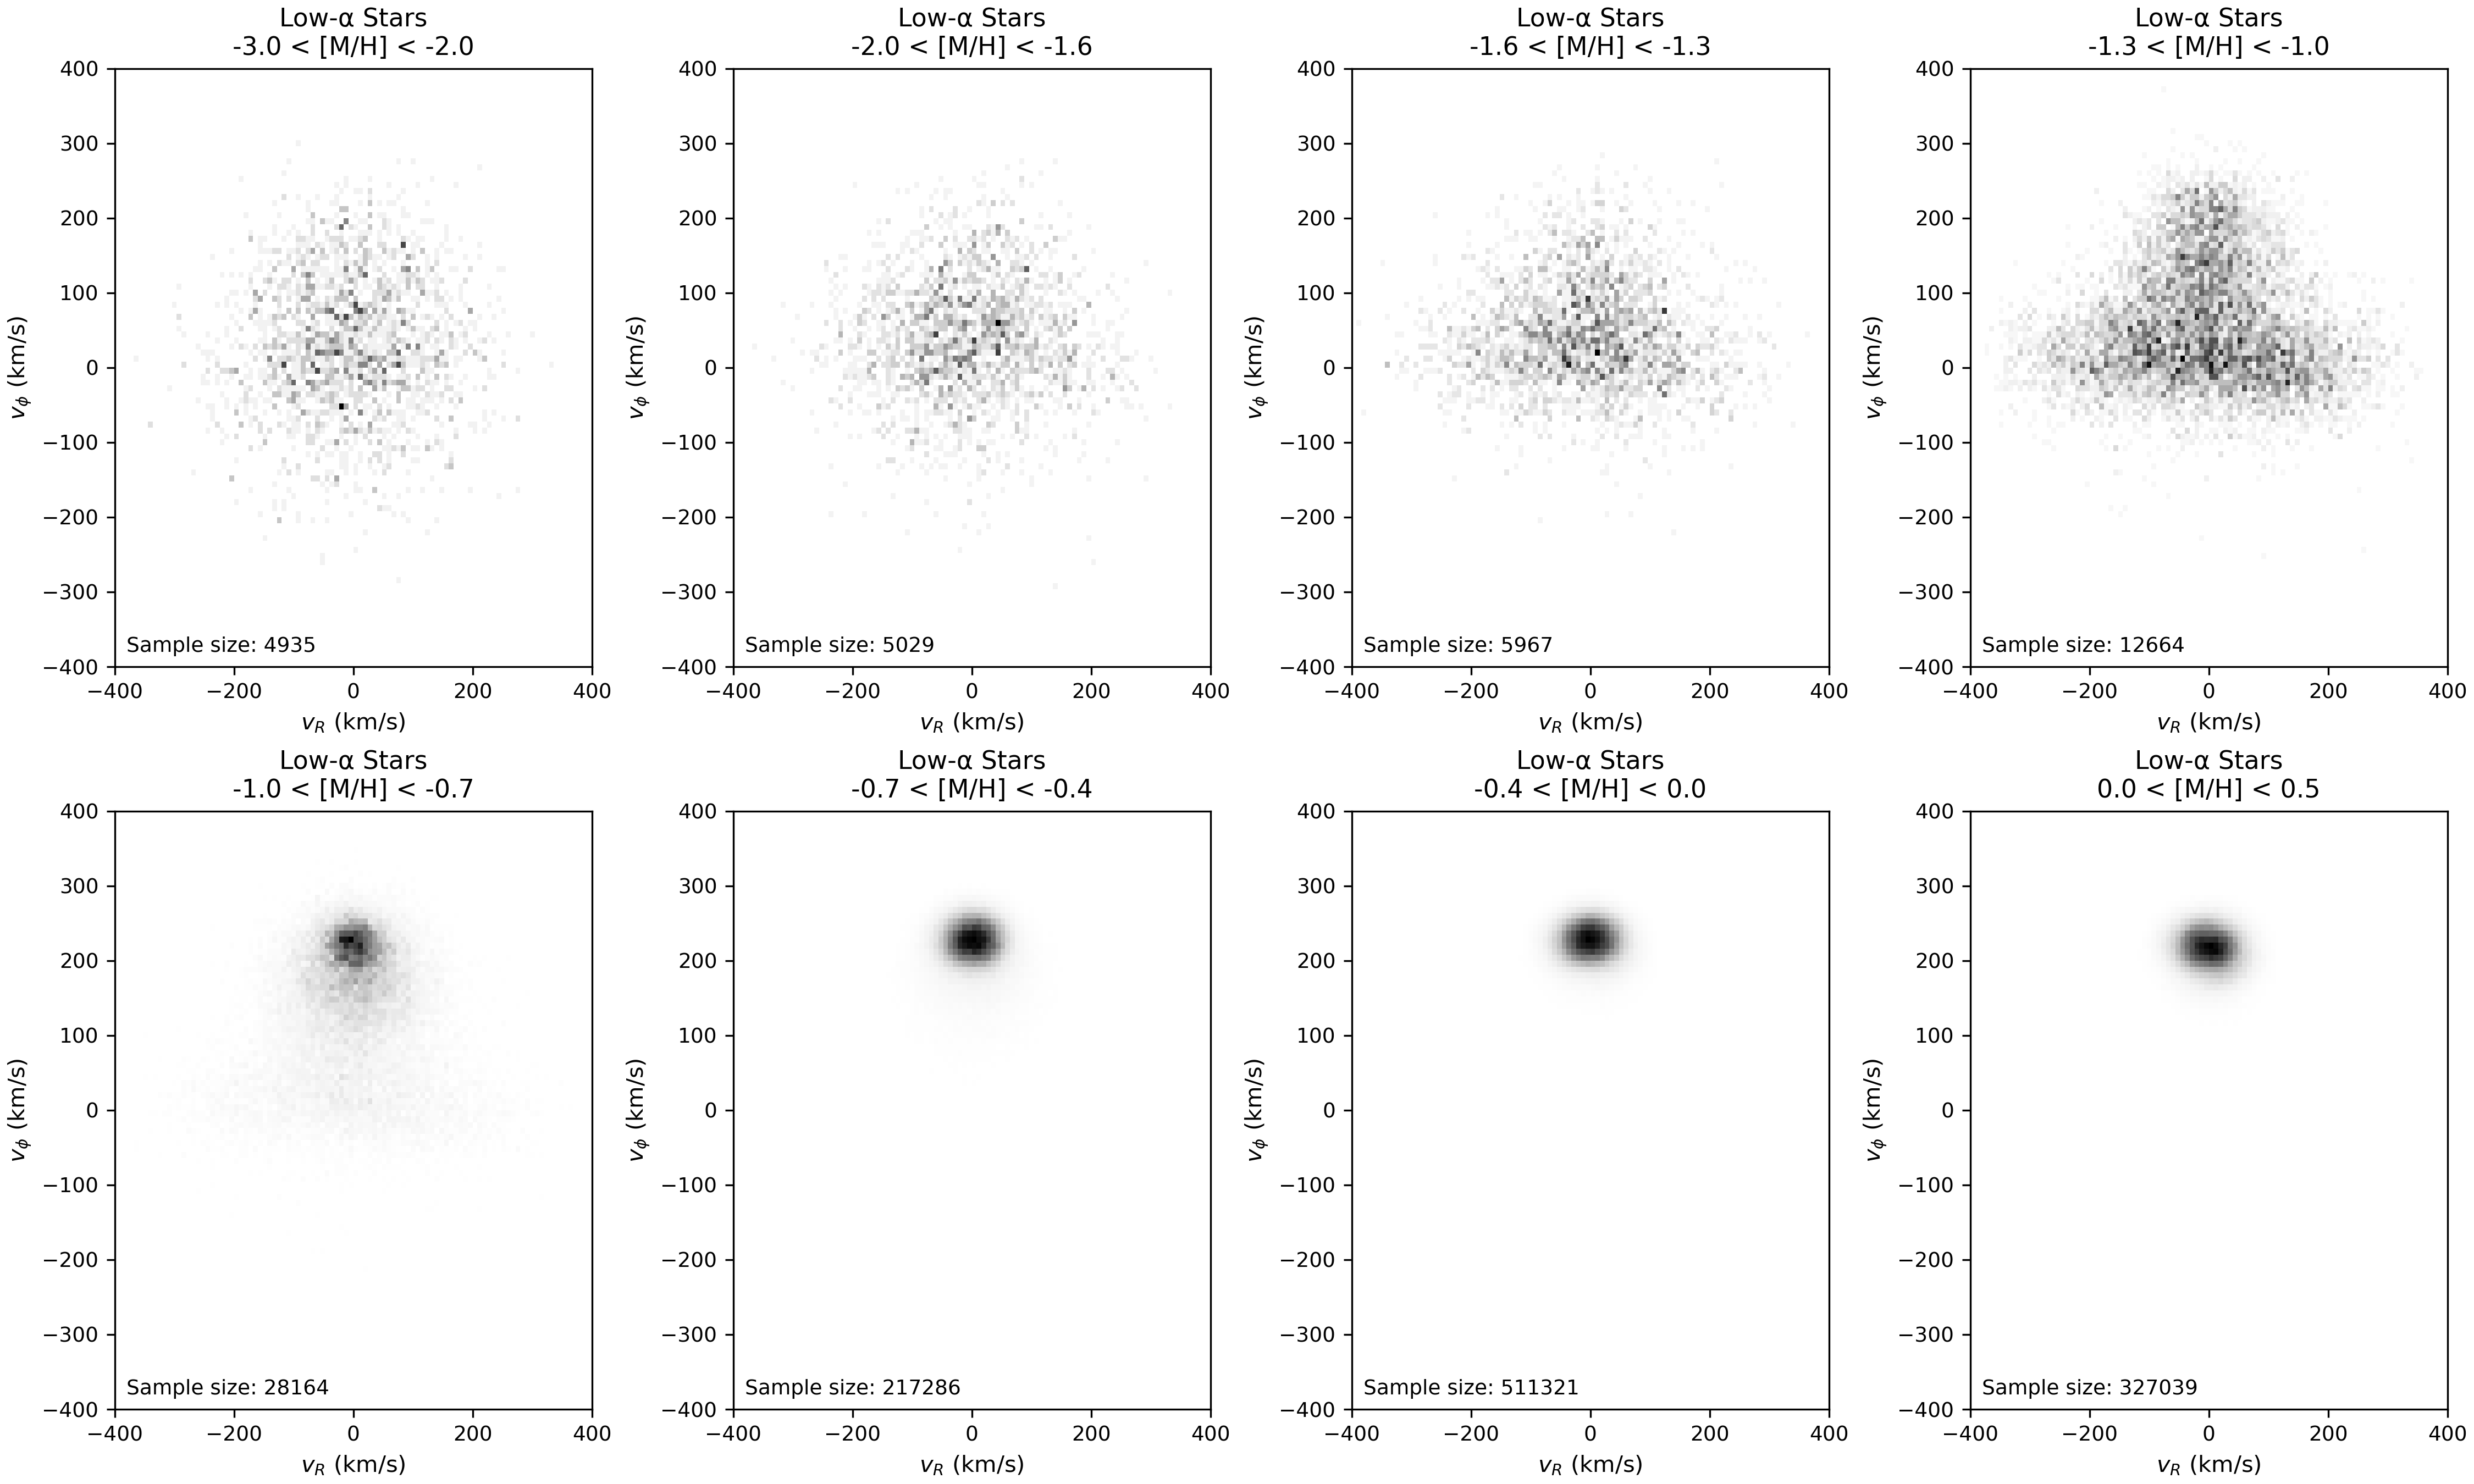
\includegraphics[width=\textwidth]{../figures/low_alpha.png}
  \caption{Distribution of stars in $v_R$–$v_\phi$ space across eight metallicity bins
           (increasing left to right, top to bottom) for the high-$\alpha$ population (top)
           and low-$\alpha$ population (bottom). The low-$\alpha$ stars are clearly more
           rotation-supported at high metallicities, while the high-$\alpha$ sample shows a
           broader velocity structure across all bins, consistent with thick-disc and halo populations.}
  \label{fig:vr_vphi_alpha}
\end{figure}

\subsection{Gaussian Mixture Model Fit}

We follow the same Gaussian mixture model fitting procedure as in
Section~\ref{subsec:gmm}, but now separately for the high- and low-$\alpha$ sequences.

\begin{table}[H]
  \centering
  \resizebox{0.95\textwidth}{!}{%
    \begin{tabular}{lcccc}
      \toprule
      $\alpha$-Sequence & VMP ($[\mathrm{M/H}]<-2.0$) & IMP ($-2.0<[\mathrm{M/H}]<-1.3$) & MP1 ($-1.3<[\mathrm{M/H}]<-1.0$) & MP2 ($-1.0<[\mathrm{M/H}]<-0.7$) \\
      \midrule
      High-$\alpha$ & 1 & 4 & 5 & 3 \\
      Low-$\alpha$  & 1 & 2 & 4 & 6 \\
      \bottomrule
    \end{tabular}
  }
  \caption{Number of Gaussian Mixture components selected by the BIC for each metallicity bin, split by $\alpha$-sequence.}
    \label{tab:gmm_components_alpha}
\end{table}

Following the methodology described in Section~\ref{subsec:n_components}, Table~\ref{tab:gmm_components_alpha} summarises the number of components selected by the Bayesian Information Criterion (BIC) for each metallicity bin.
It shows that both $\alpha$–sequences are well-described by a single broad Gaussian in the very–metal–poor (VMP) bin, consistent with a pressure–supported halo.  
With increasing metallicity the low–$\alpha$ branch adds components gradually (1\,$\rightarrow$\,2\,$\rightarrow$\,4\,$\rightarrow$\,6), reflecting the orderly emergence of a thin–disc peak and its progressively colder tail.  
The high–$\alpha$ stars, in contrast, already require four Gaussians in the intermediate-metallicity bin (IMP) and peak at five in MP1 before contracting to three in the metal-rich MP2 interval ($-1.0<\mathrm{[M/H]}<-0.7$).

\begin{figure*}[htbp]
    \centering

    % High-alpha row
    \begin{subfigure}[t]{0.24\textwidth}
        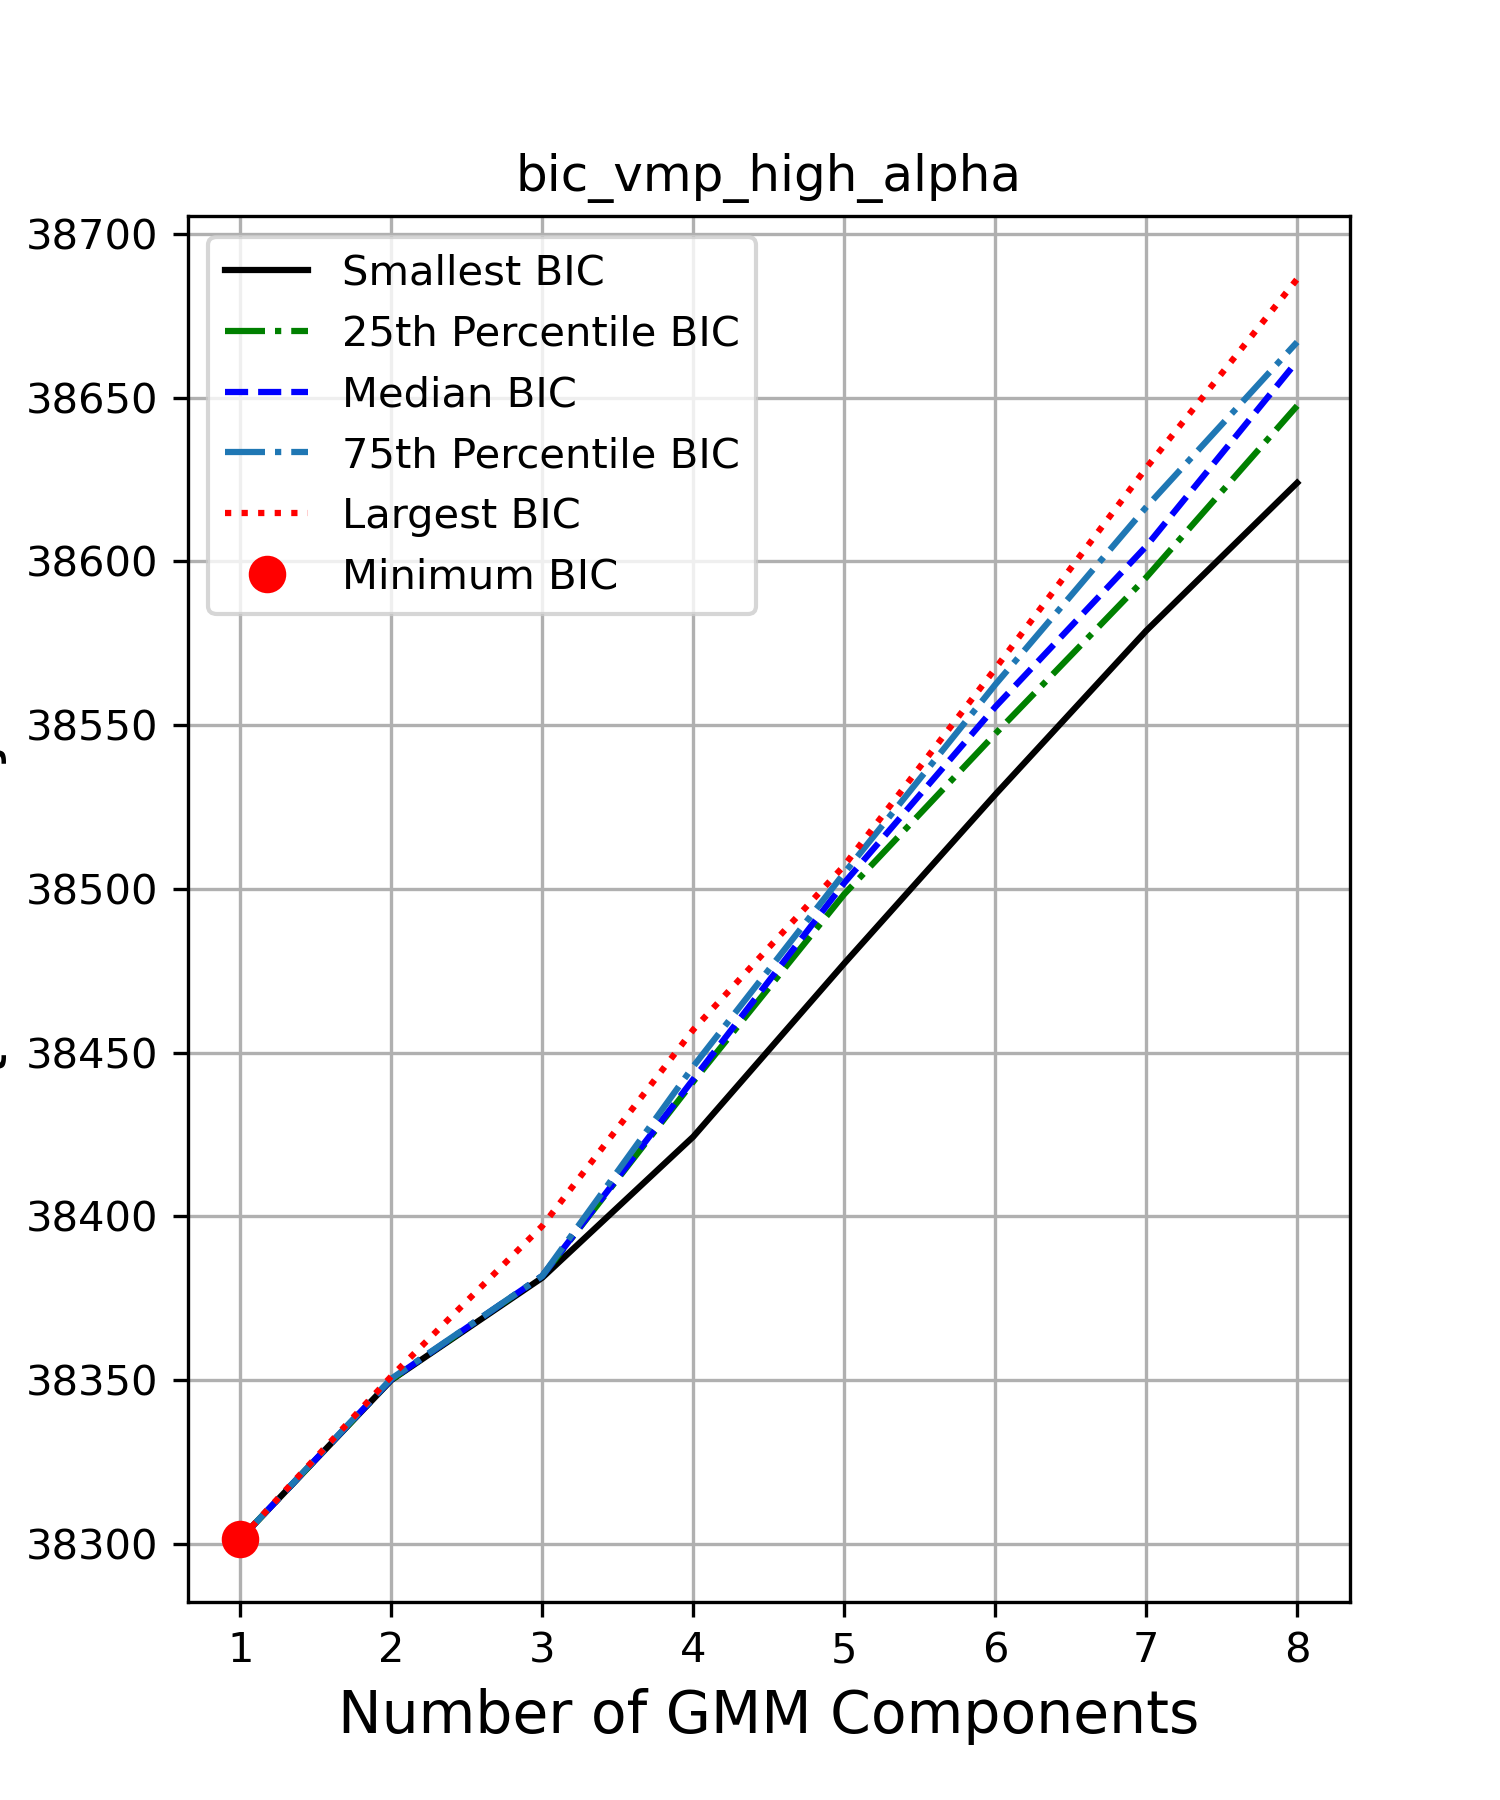
\includegraphics[width=\textwidth]{../figures/bic_vmp_high_alpha.png}
        \caption{High-$\alpha$ VMP}
    \end{subfigure}
    \begin{subfigure}[t]{0.24\textwidth}
        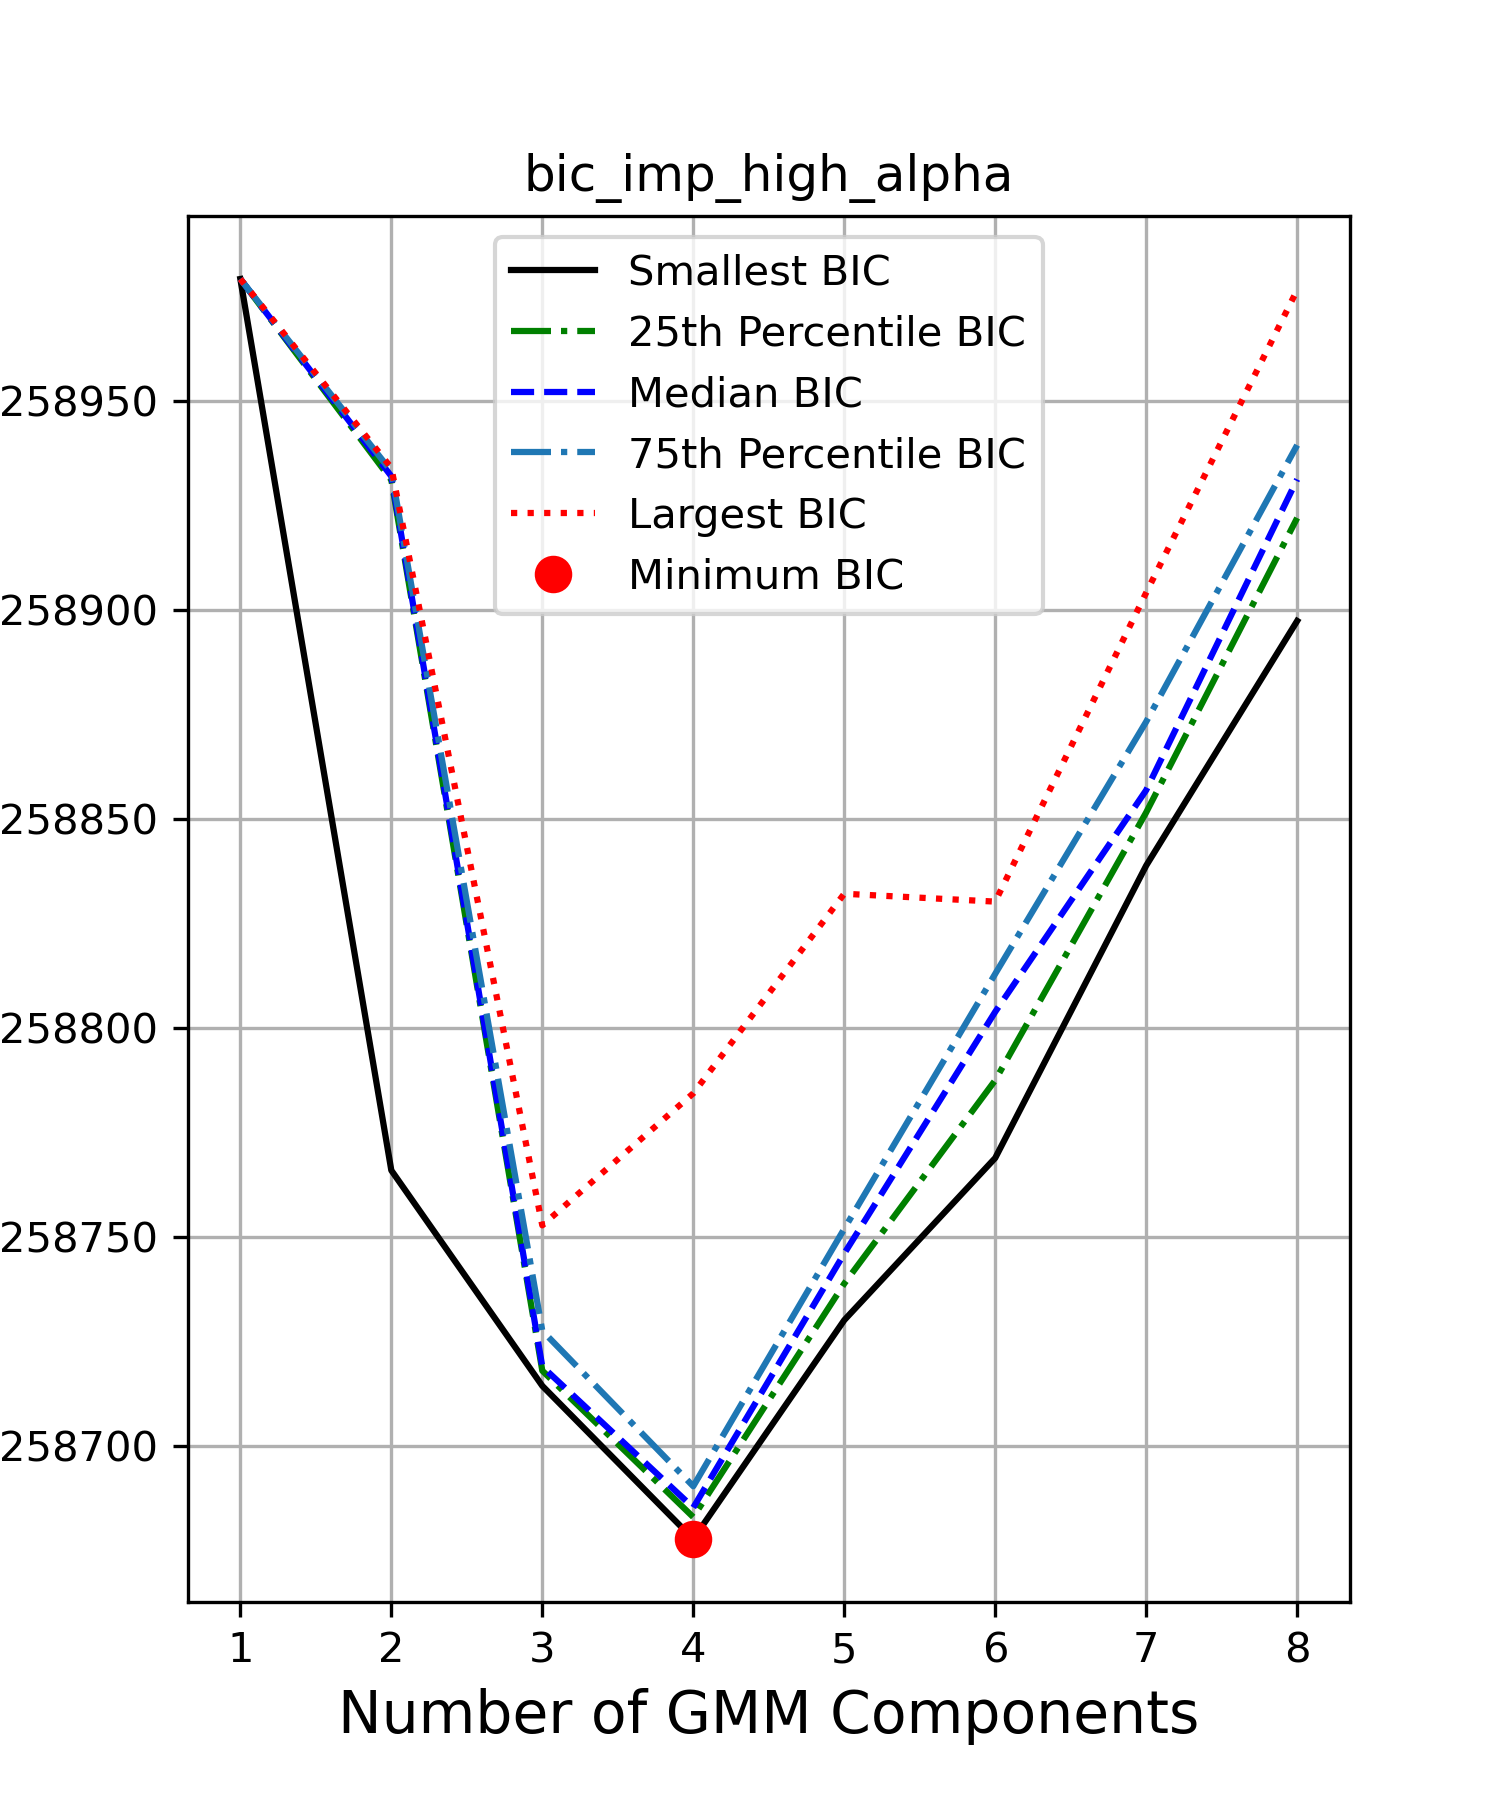
\includegraphics[width=\textwidth]{../figures/bic_imp_high_alpha.png}
        \caption{High-$\alpha$ IMP}
    \end{subfigure}
    \begin{subfigure}[t]{0.24\textwidth}
        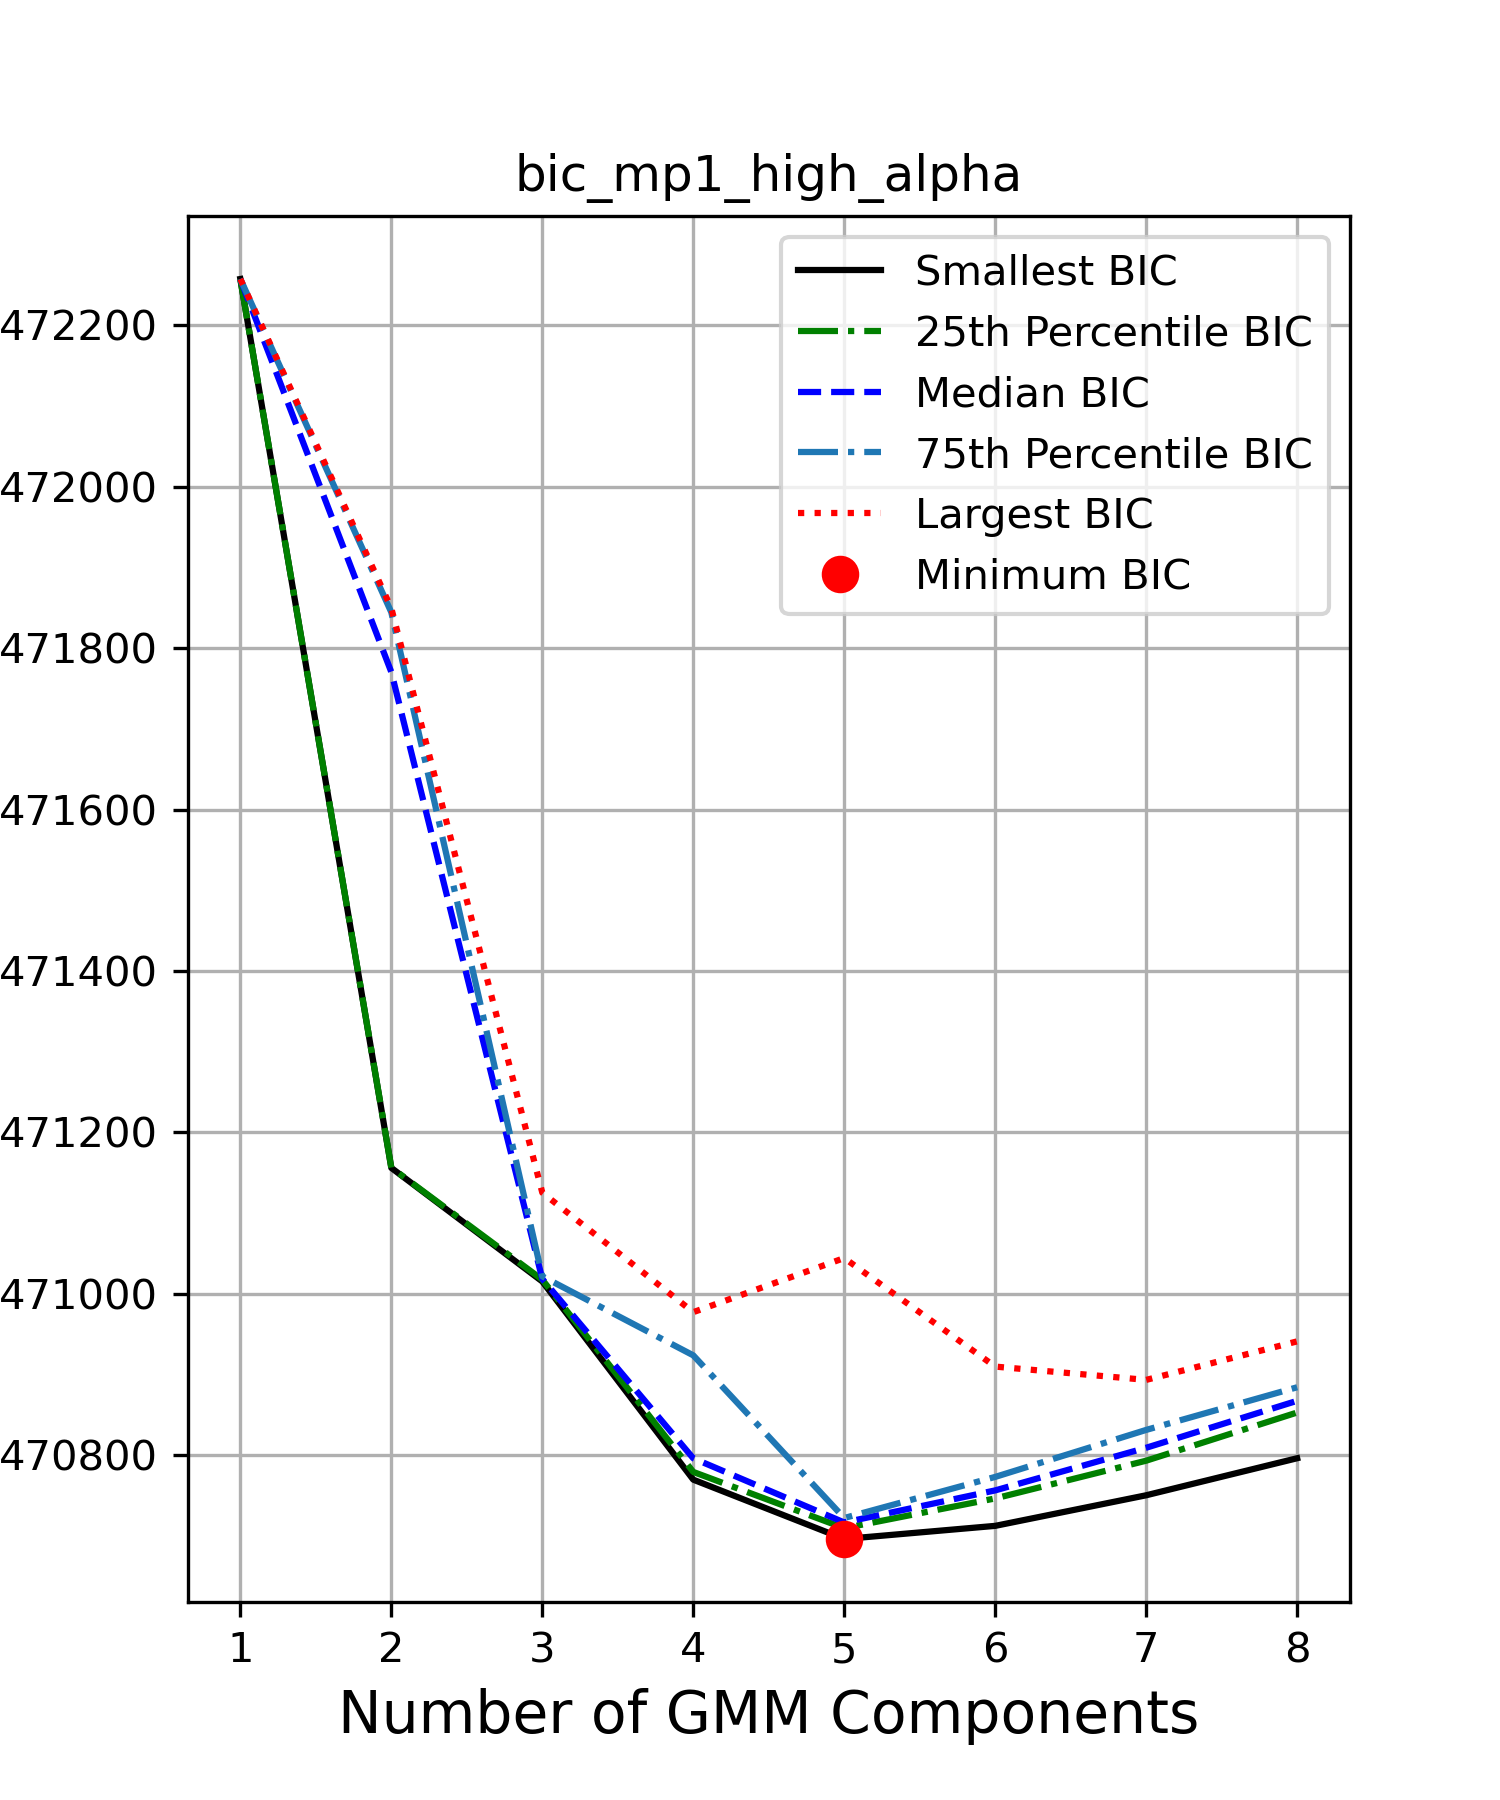
\includegraphics[width=\textwidth]{../figures/bic_mp1_high_alpha.png}
        \caption{High-$\alpha$ MP1}
    \end{subfigure}
    \begin{subfigure}[t]{0.24\textwidth}
        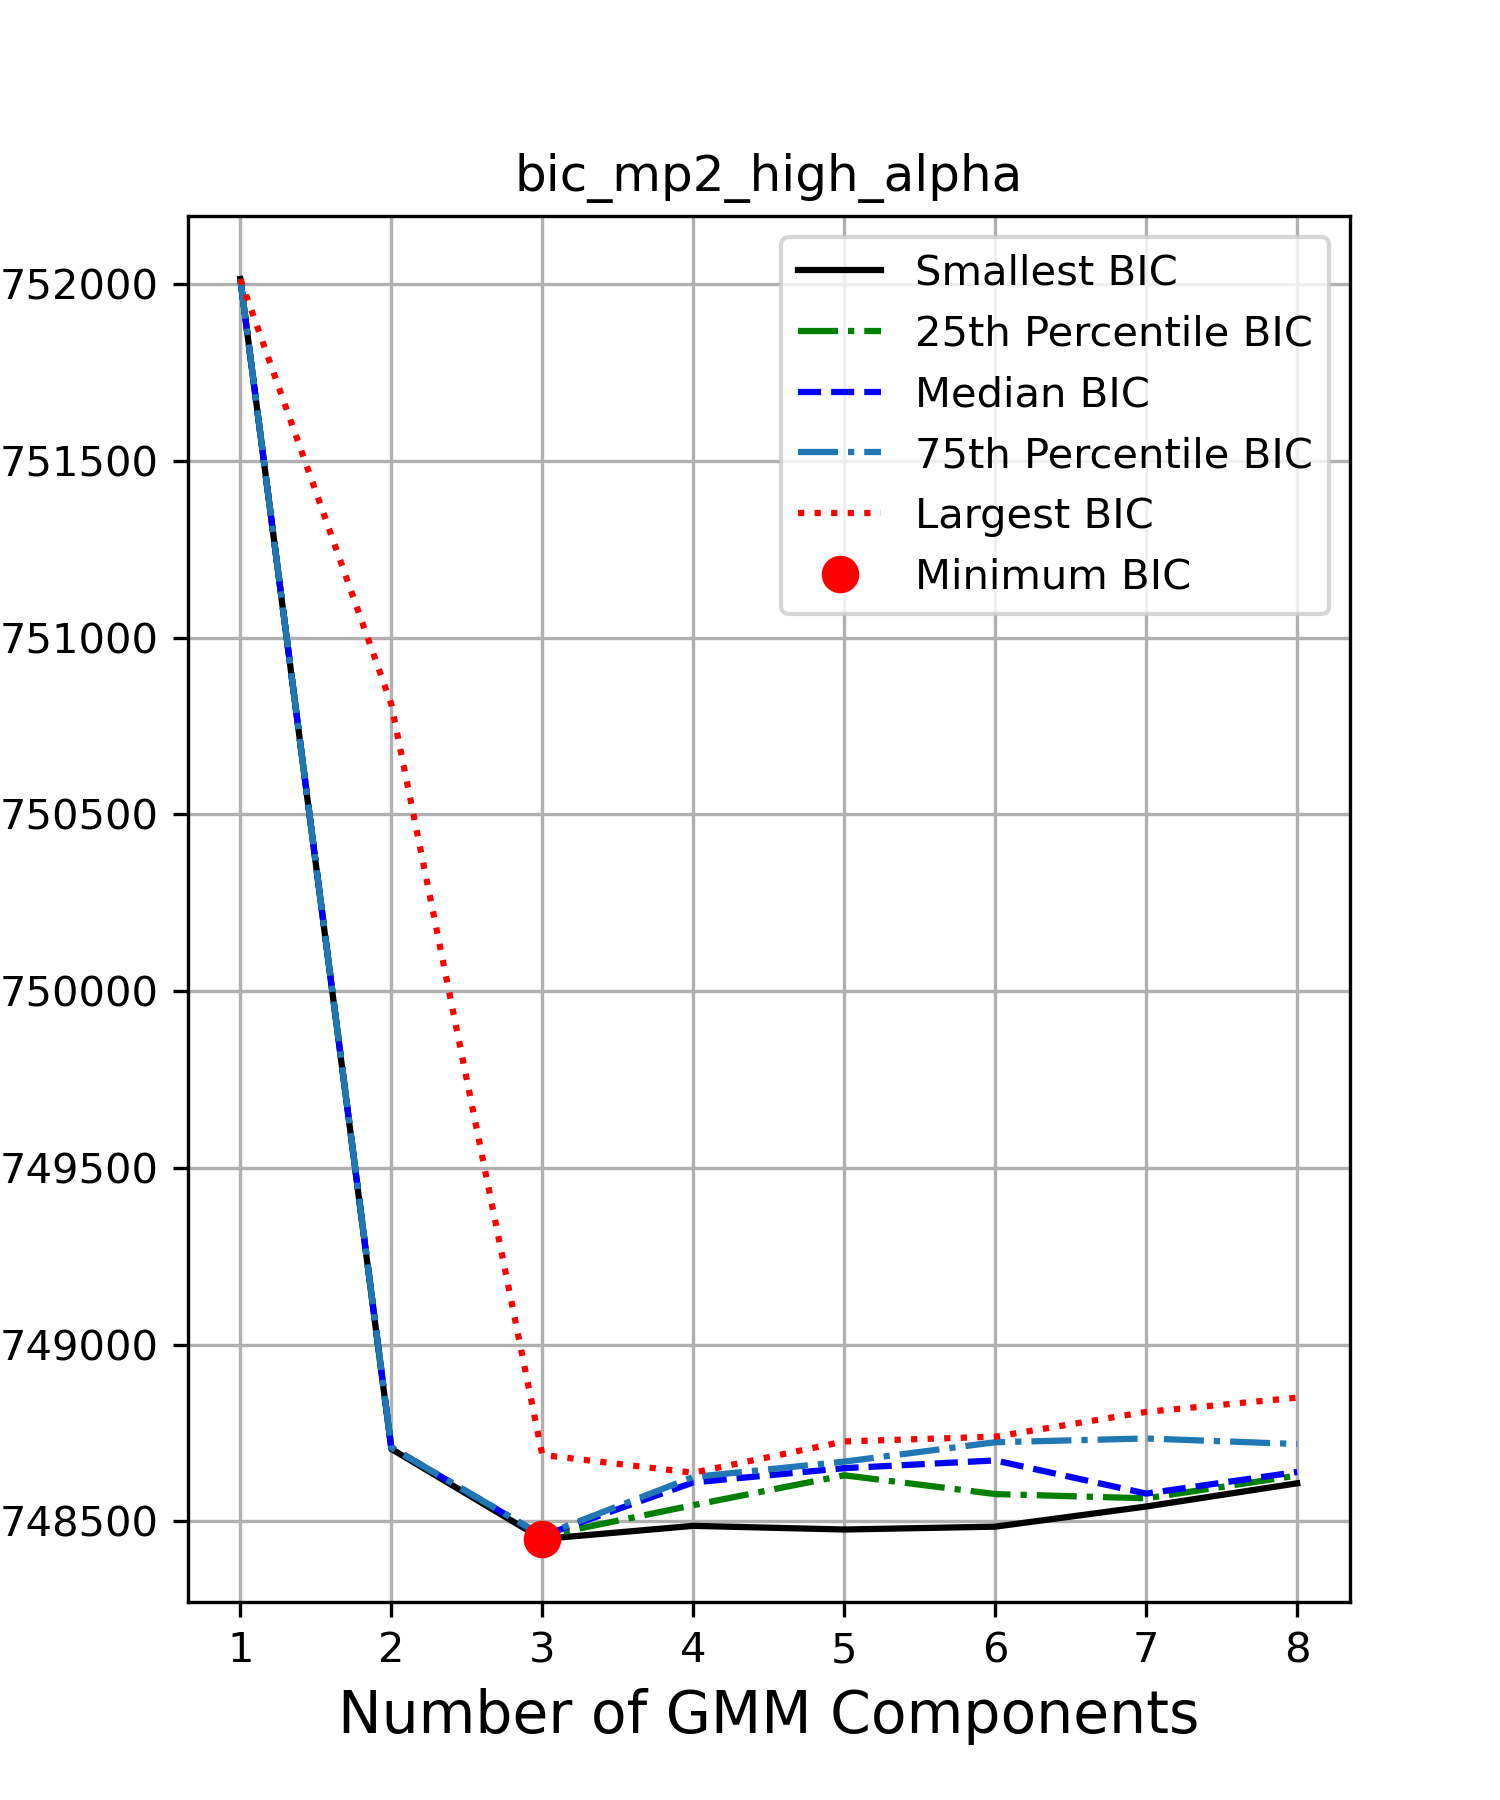
\includegraphics[width=\textwidth]{../figures/bic_mp2_high_alpha.png}
        \caption{High-$\alpha$ MP2}
    \end{subfigure}

    \vspace{0.5em}

    % Low-alpha row
    \begin{subfigure}[t]{0.24\textwidth}
        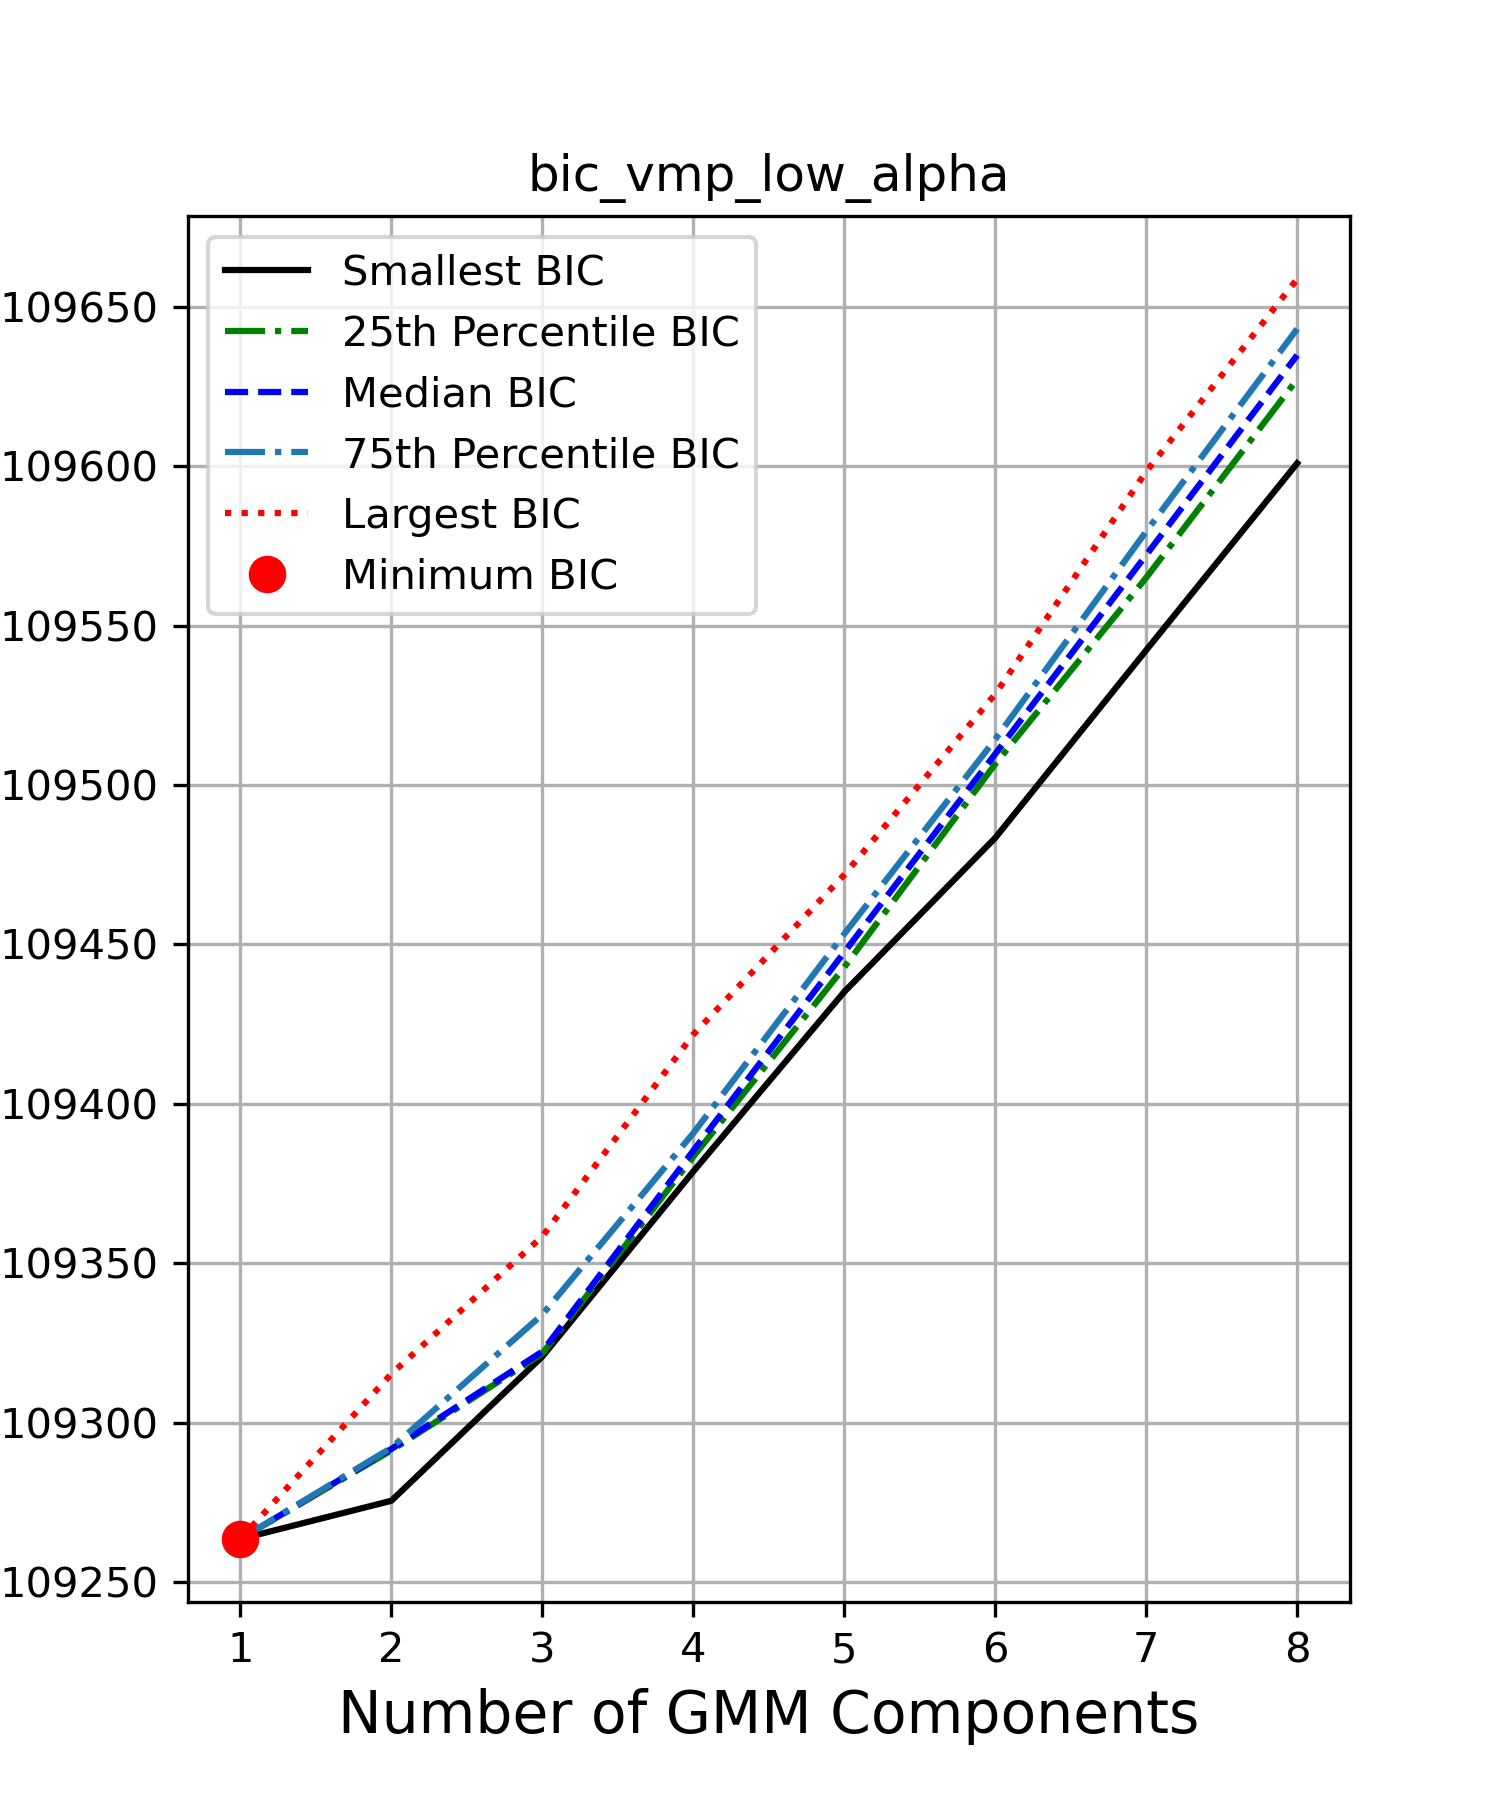
\includegraphics[width=\textwidth]{../figures/bic_vmp_low_alpha.png}
        \caption{Low-$\alpha$ VMP}
    \end{subfigure}
    \begin{subfigure}[t]{0.24\textwidth}
        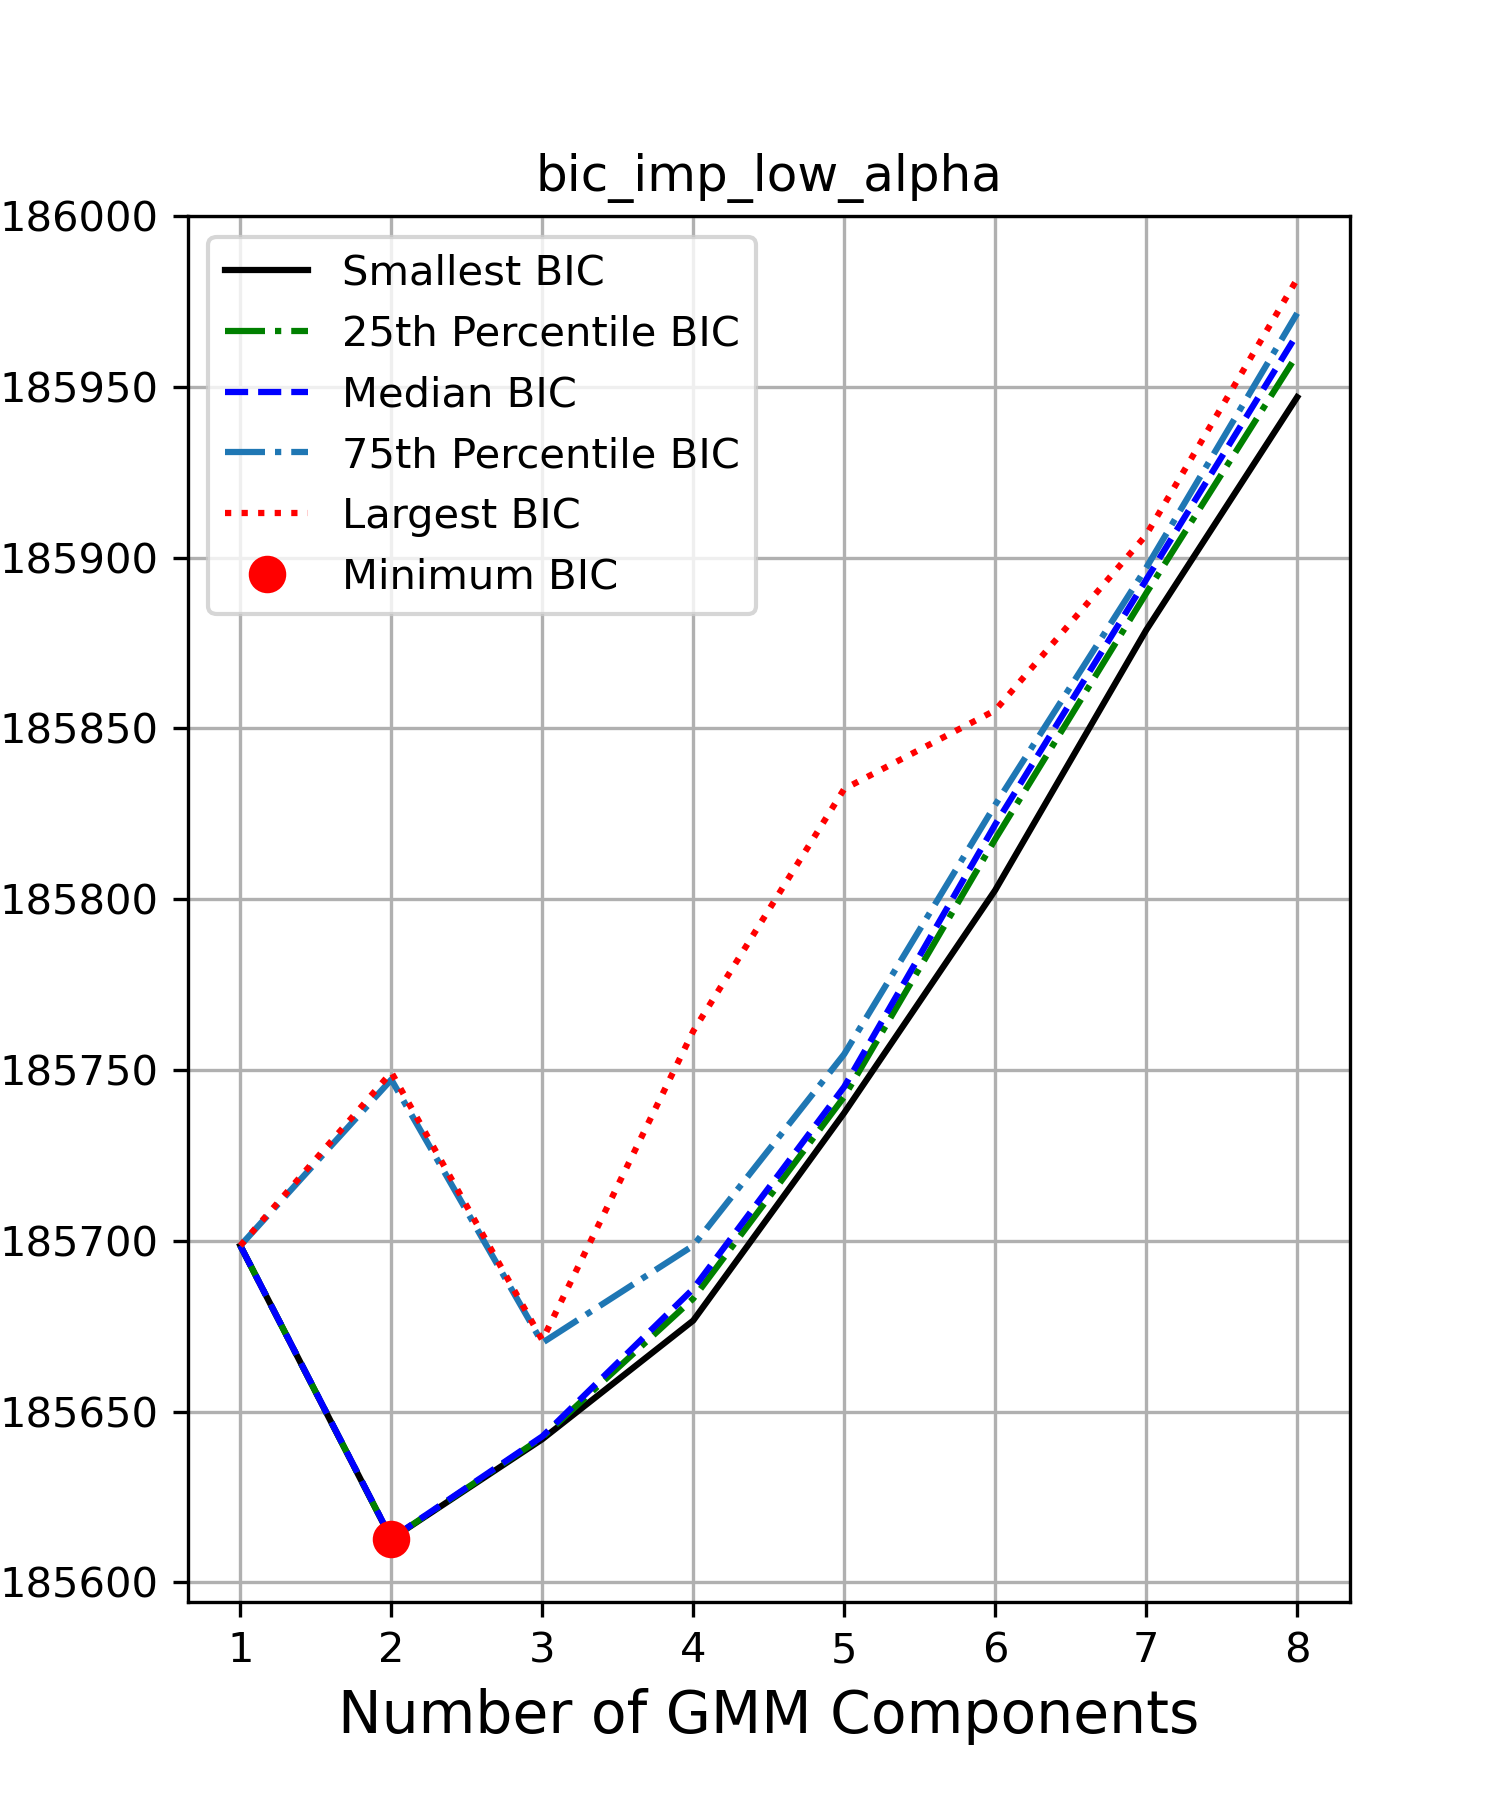
\includegraphics[width=\textwidth]{../figures/bic_imp_low_alpha.png}
        \caption{Low-$\alpha$ IMP}
    \end{subfigure}
    \begin{subfigure}[t]{0.24\textwidth}
        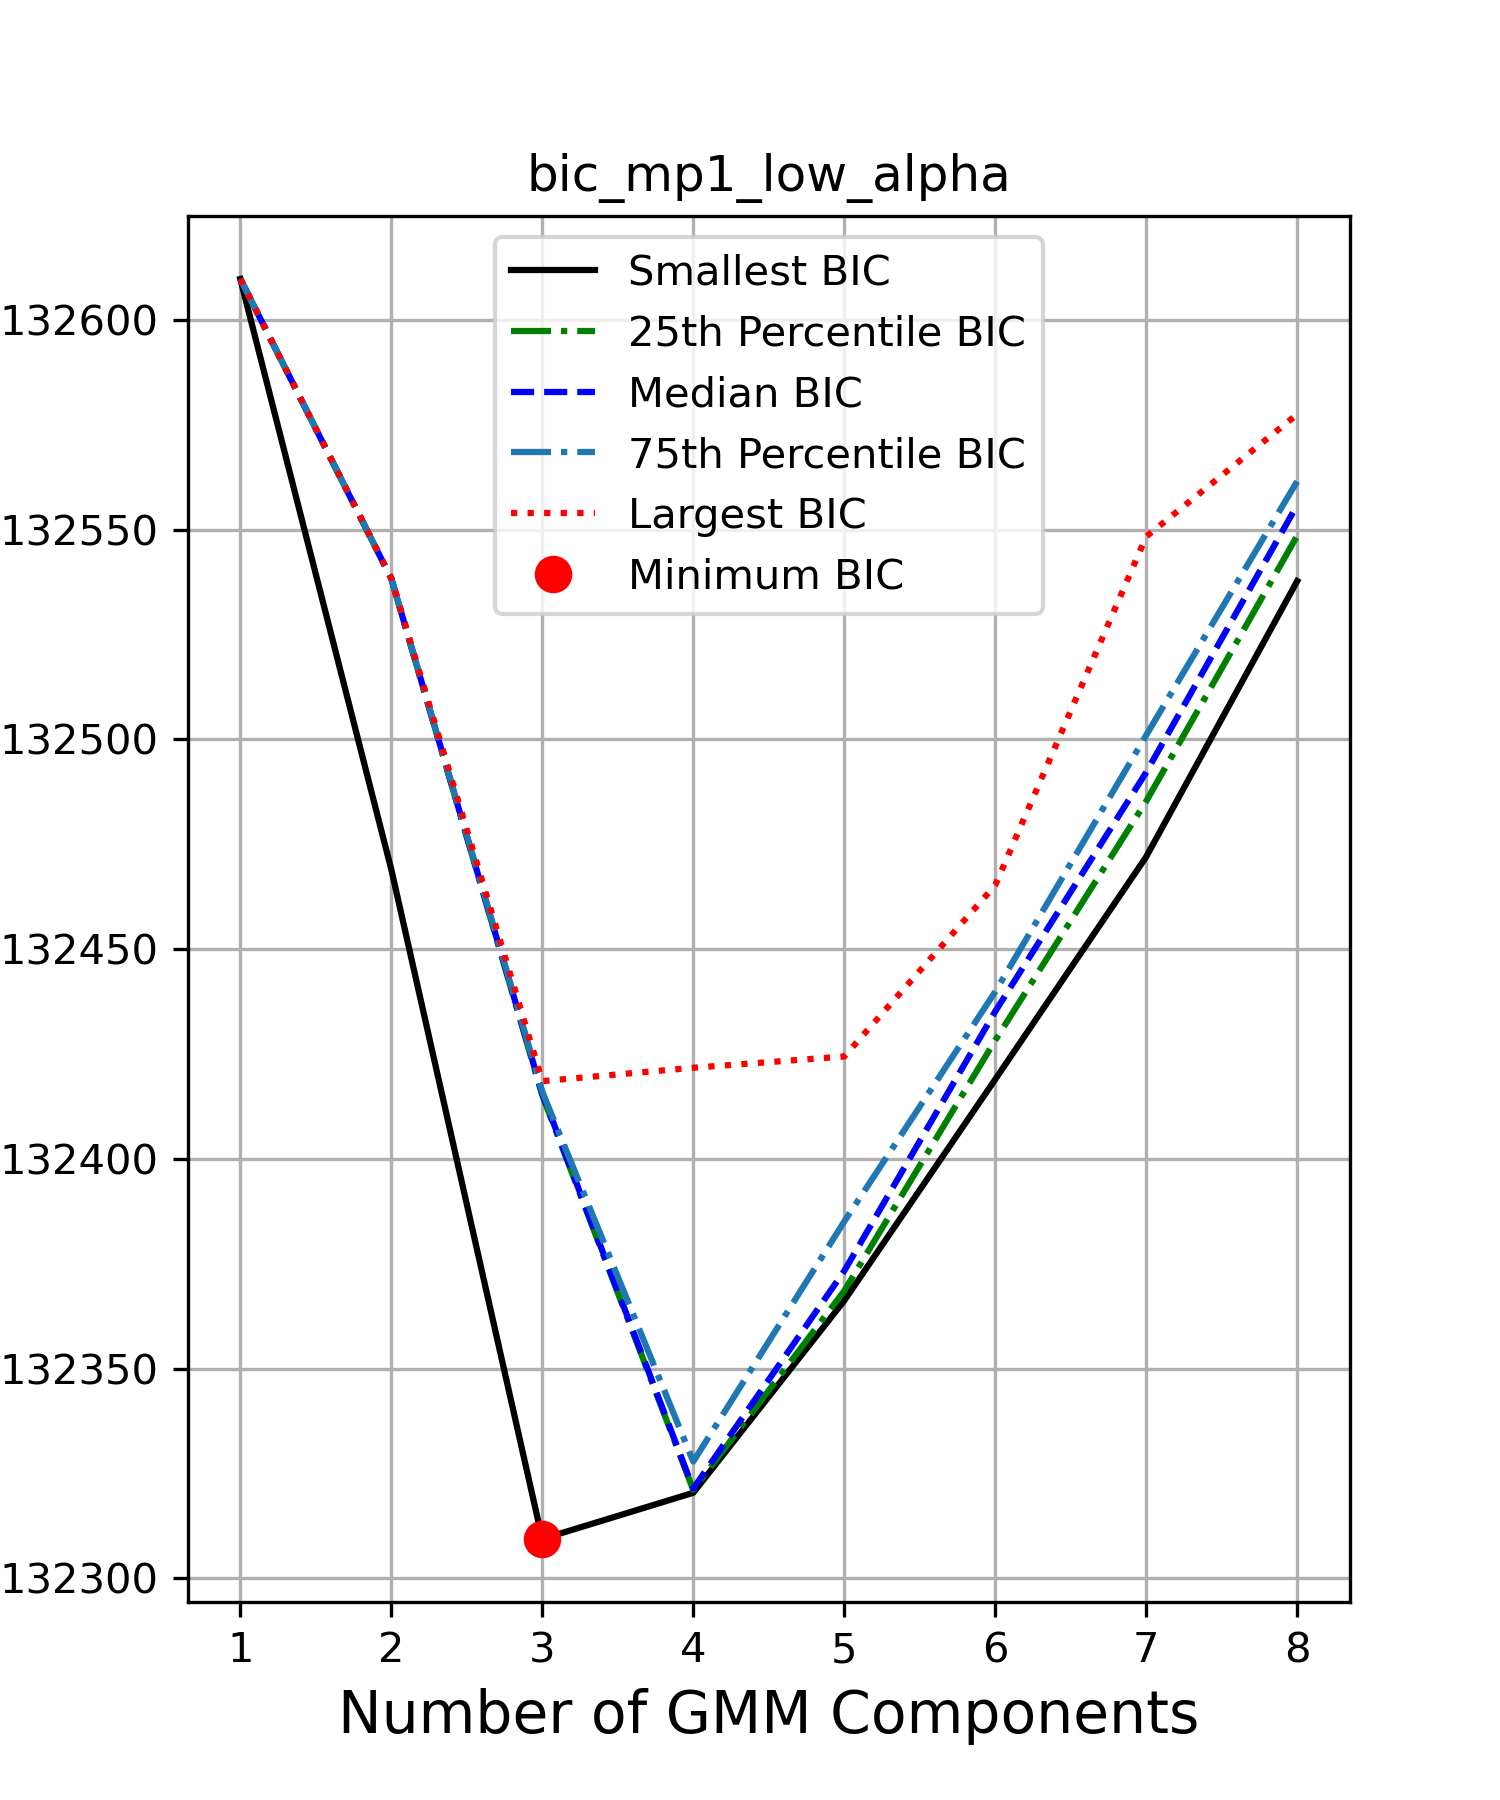
\includegraphics[width=\textwidth]{../figures/bic_mp1_low_alpha.png}
        \caption{Low-$\alpha$ MP1}
    \end{subfigure}
    \begin{subfigure}[t]{0.24\textwidth}
        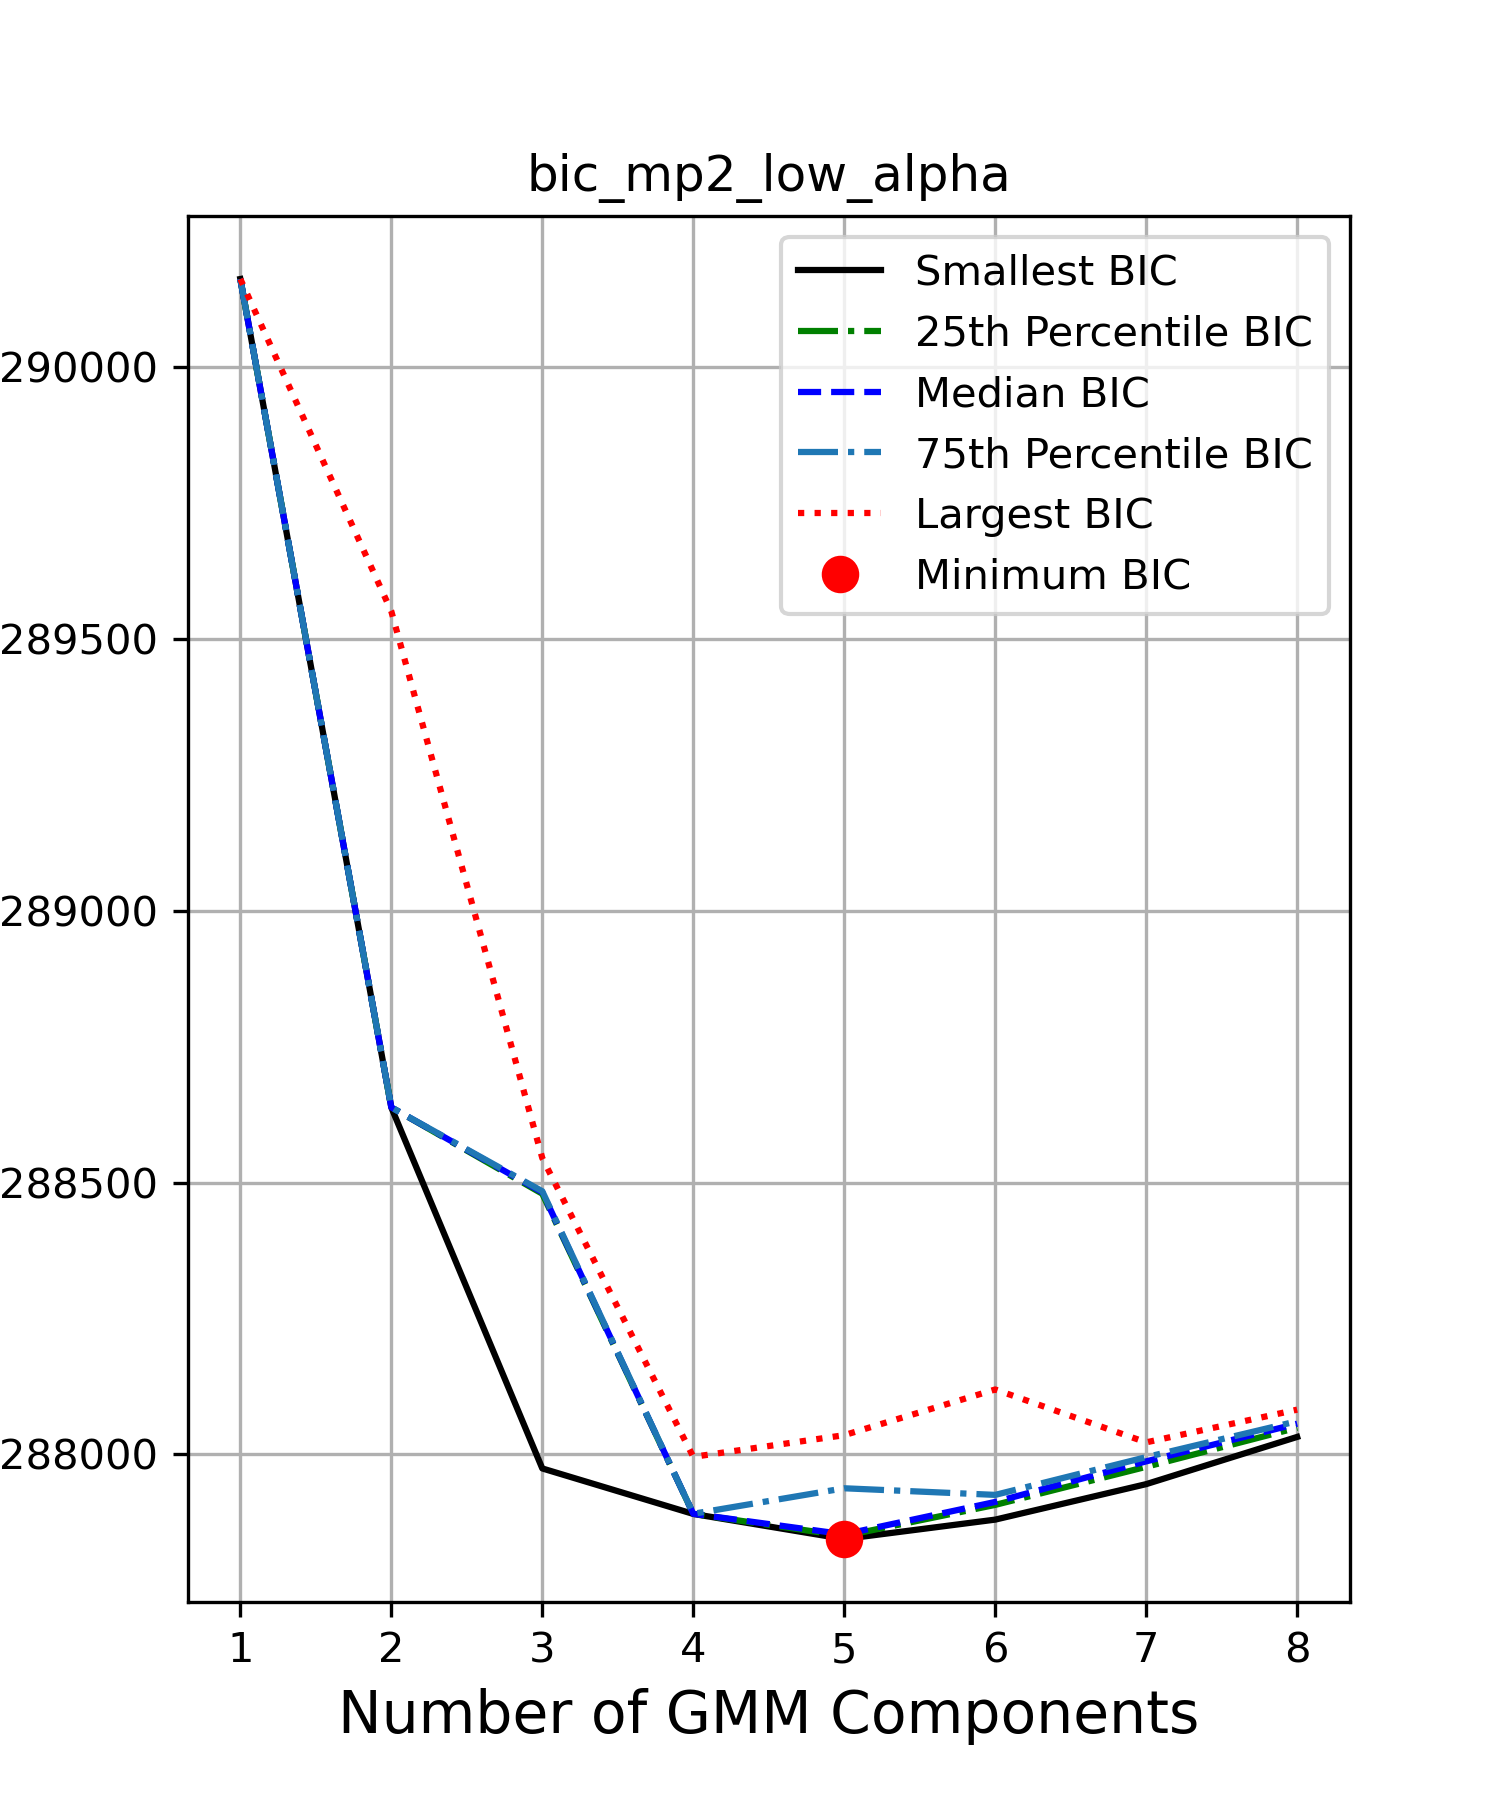
\includegraphics[width=\textwidth]{../figures/bic_mp2_low_alpha.png}
        \caption{Low-$\alpha$ MP2}
    \end{subfigure}

    \caption{BIC scores for different metallicity bins, grouped by high- and low-$\alpha$ populations.}
    \label{fig:bic_grid}
\end{figure*}


\subsection{High alpha Gaussian Mixture Model Fit}

\begin{figure}[H]
  \centering

  \begin{subfigure}{0.245\linewidth}
    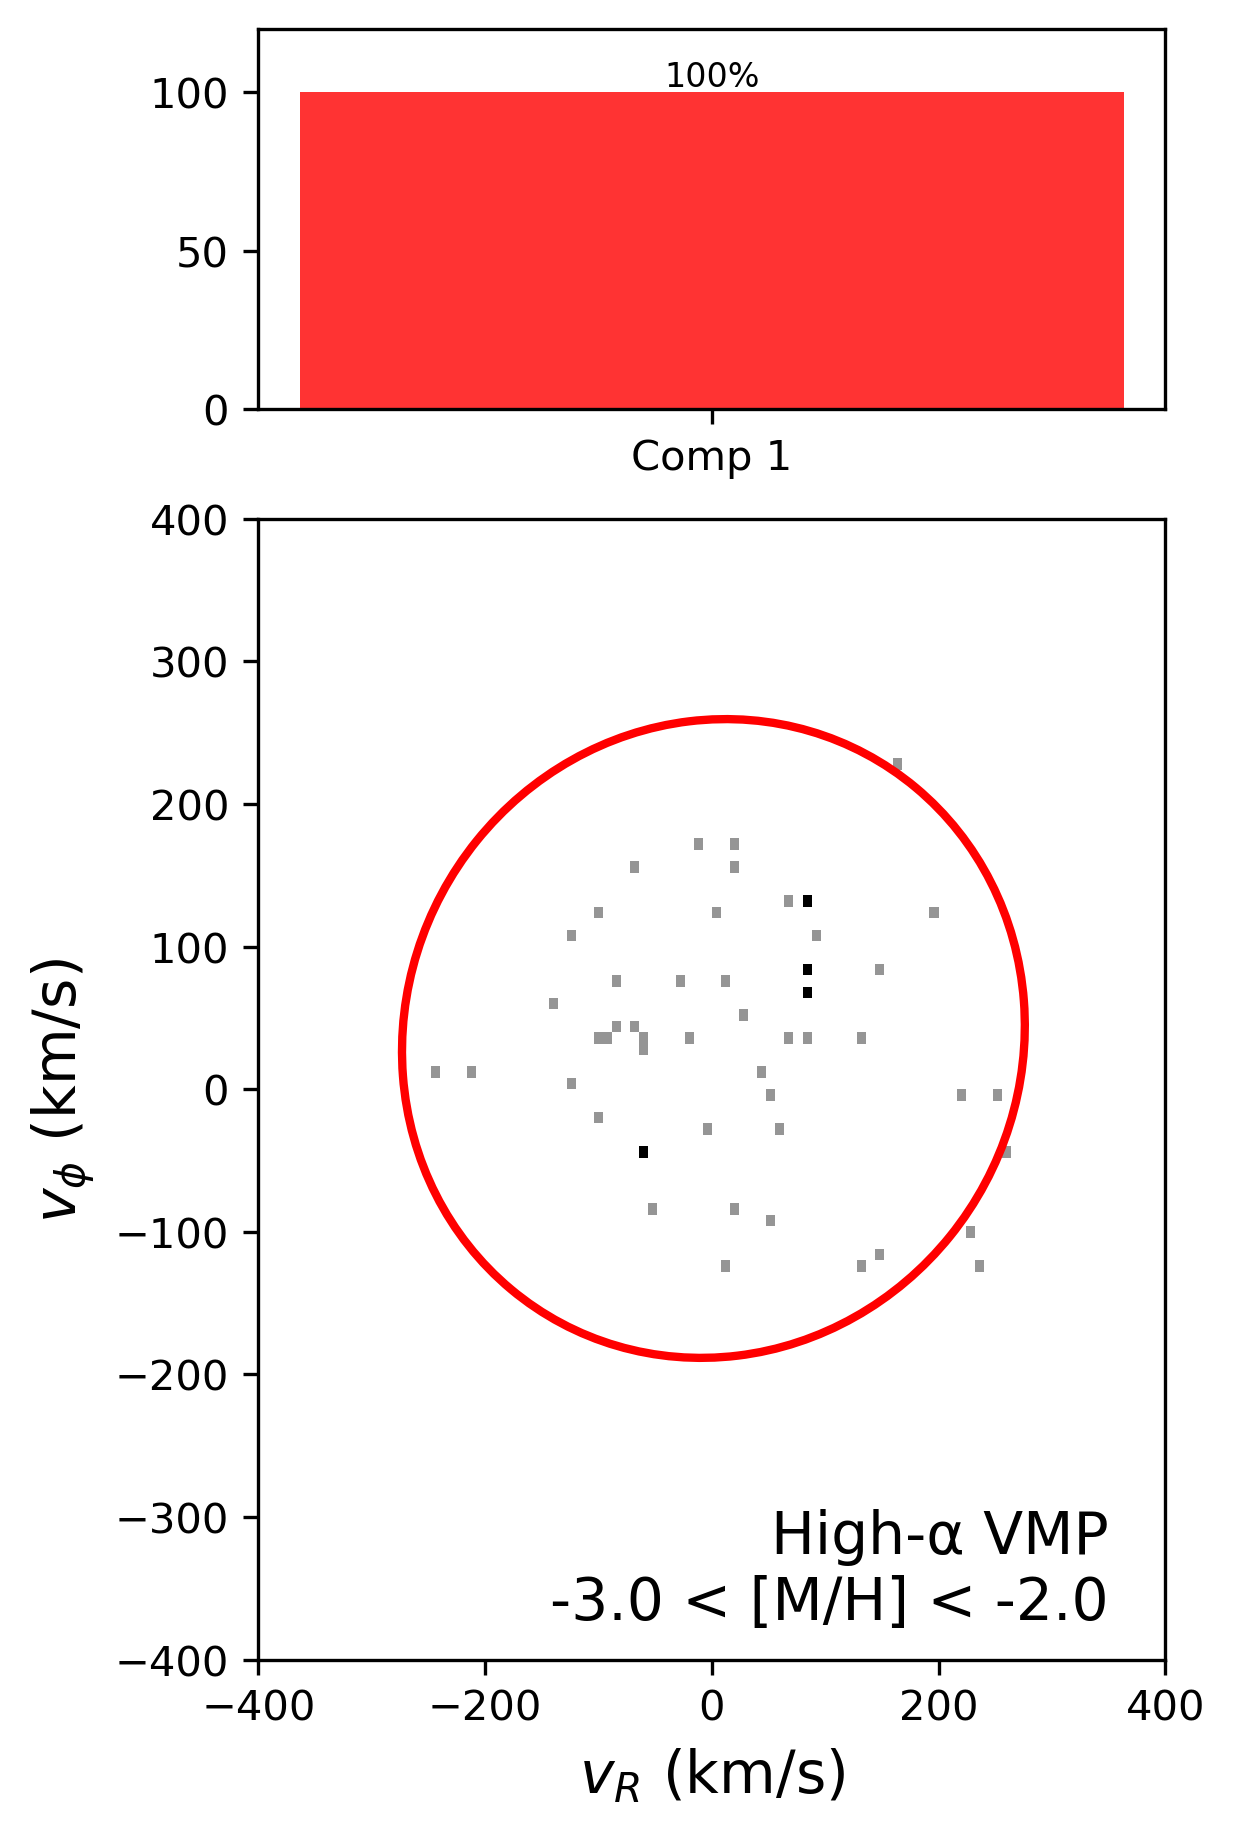
\includegraphics[width=\linewidth]{../figures/gmm_vmp_high_alpha_k1.png}
    \caption{VMP ($k{=}1$)}
    \label{fig:vmp_hi}
  \end{subfigure}\hfill
  \begin{subfigure}{0.245\linewidth}
    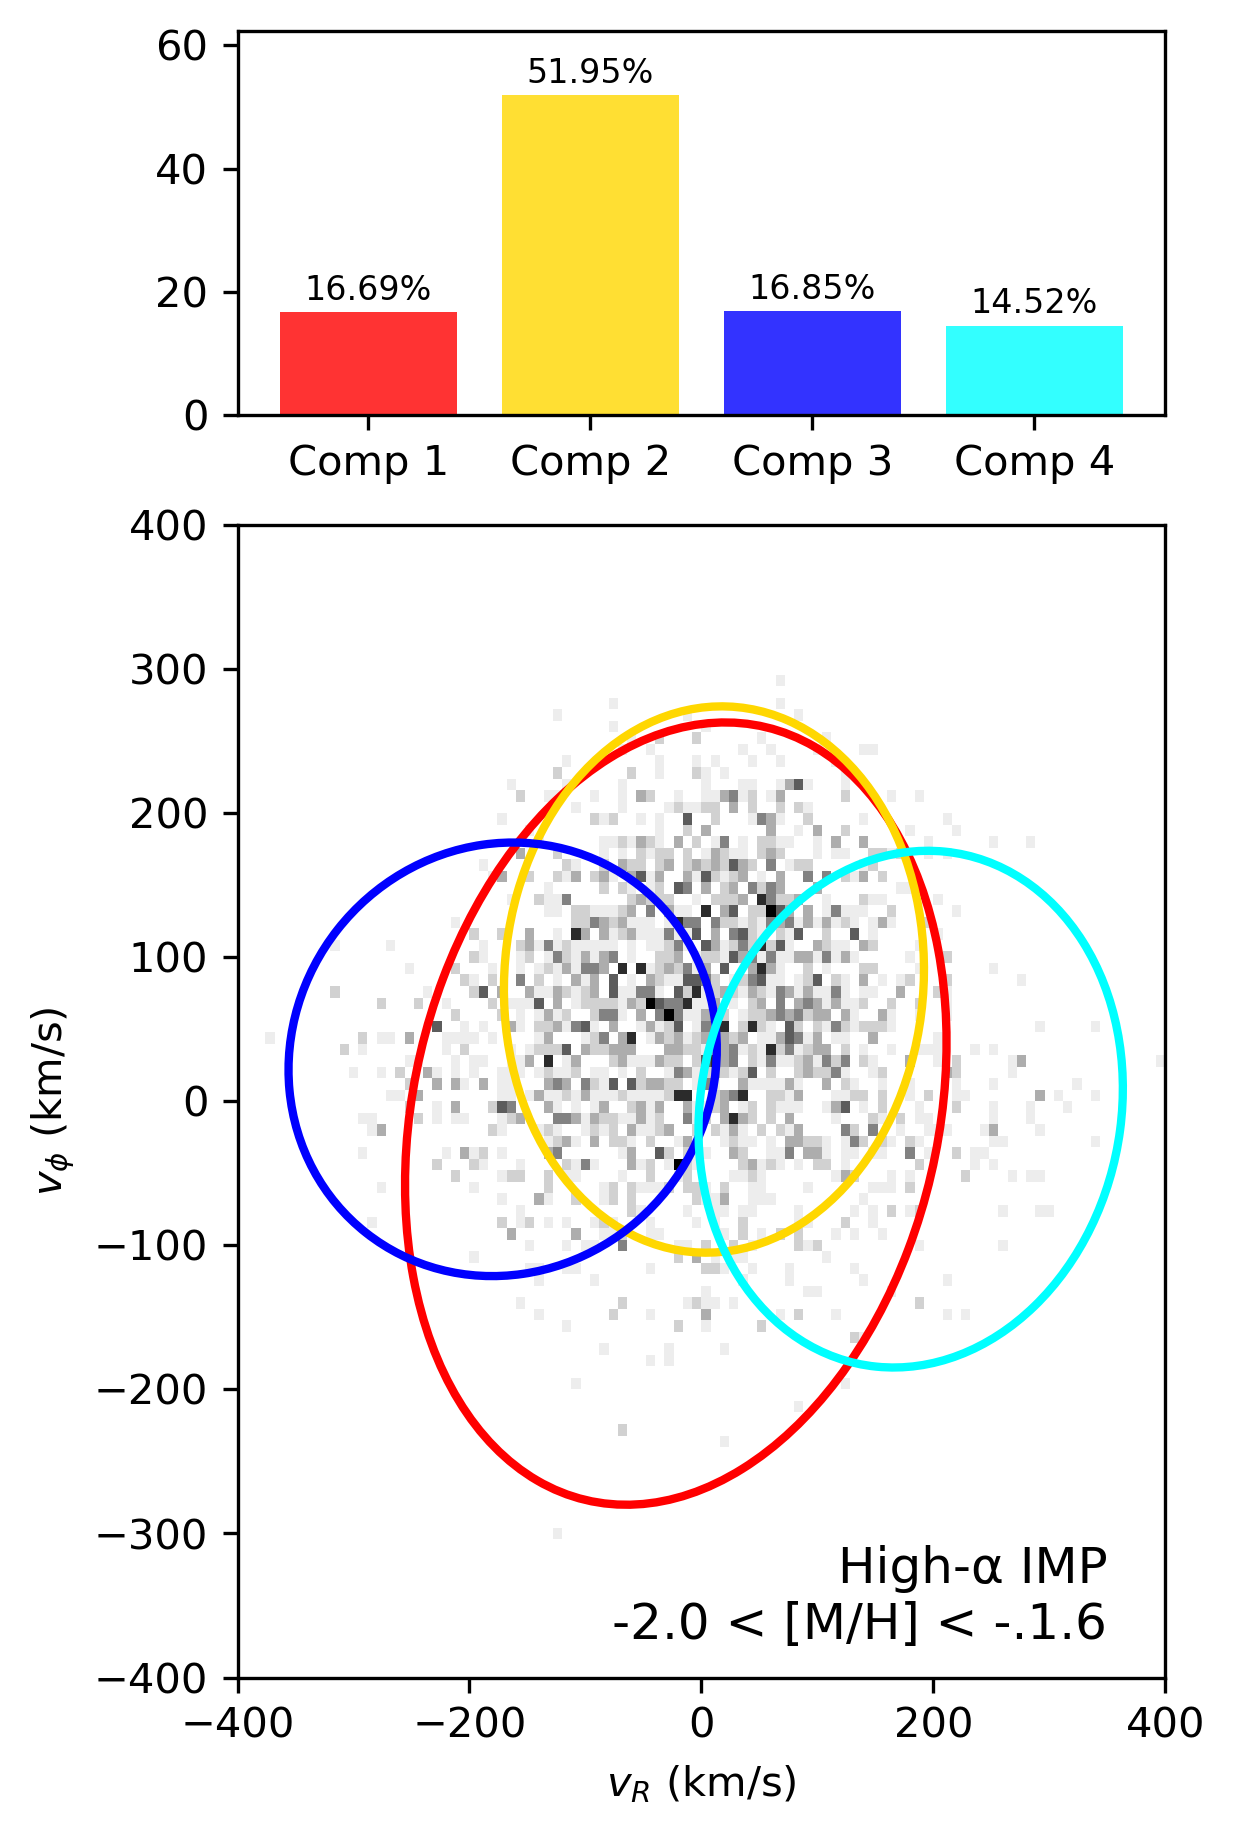
\includegraphics[width=\linewidth]{../figures/gmm_imp_high_alpha_k4.png}
    \caption{IMP ($k{=}4$)}
    \label{fig:imp_hi}
  \end{subfigure}\hfill
  \begin{subfigure}{0.245\linewidth}
    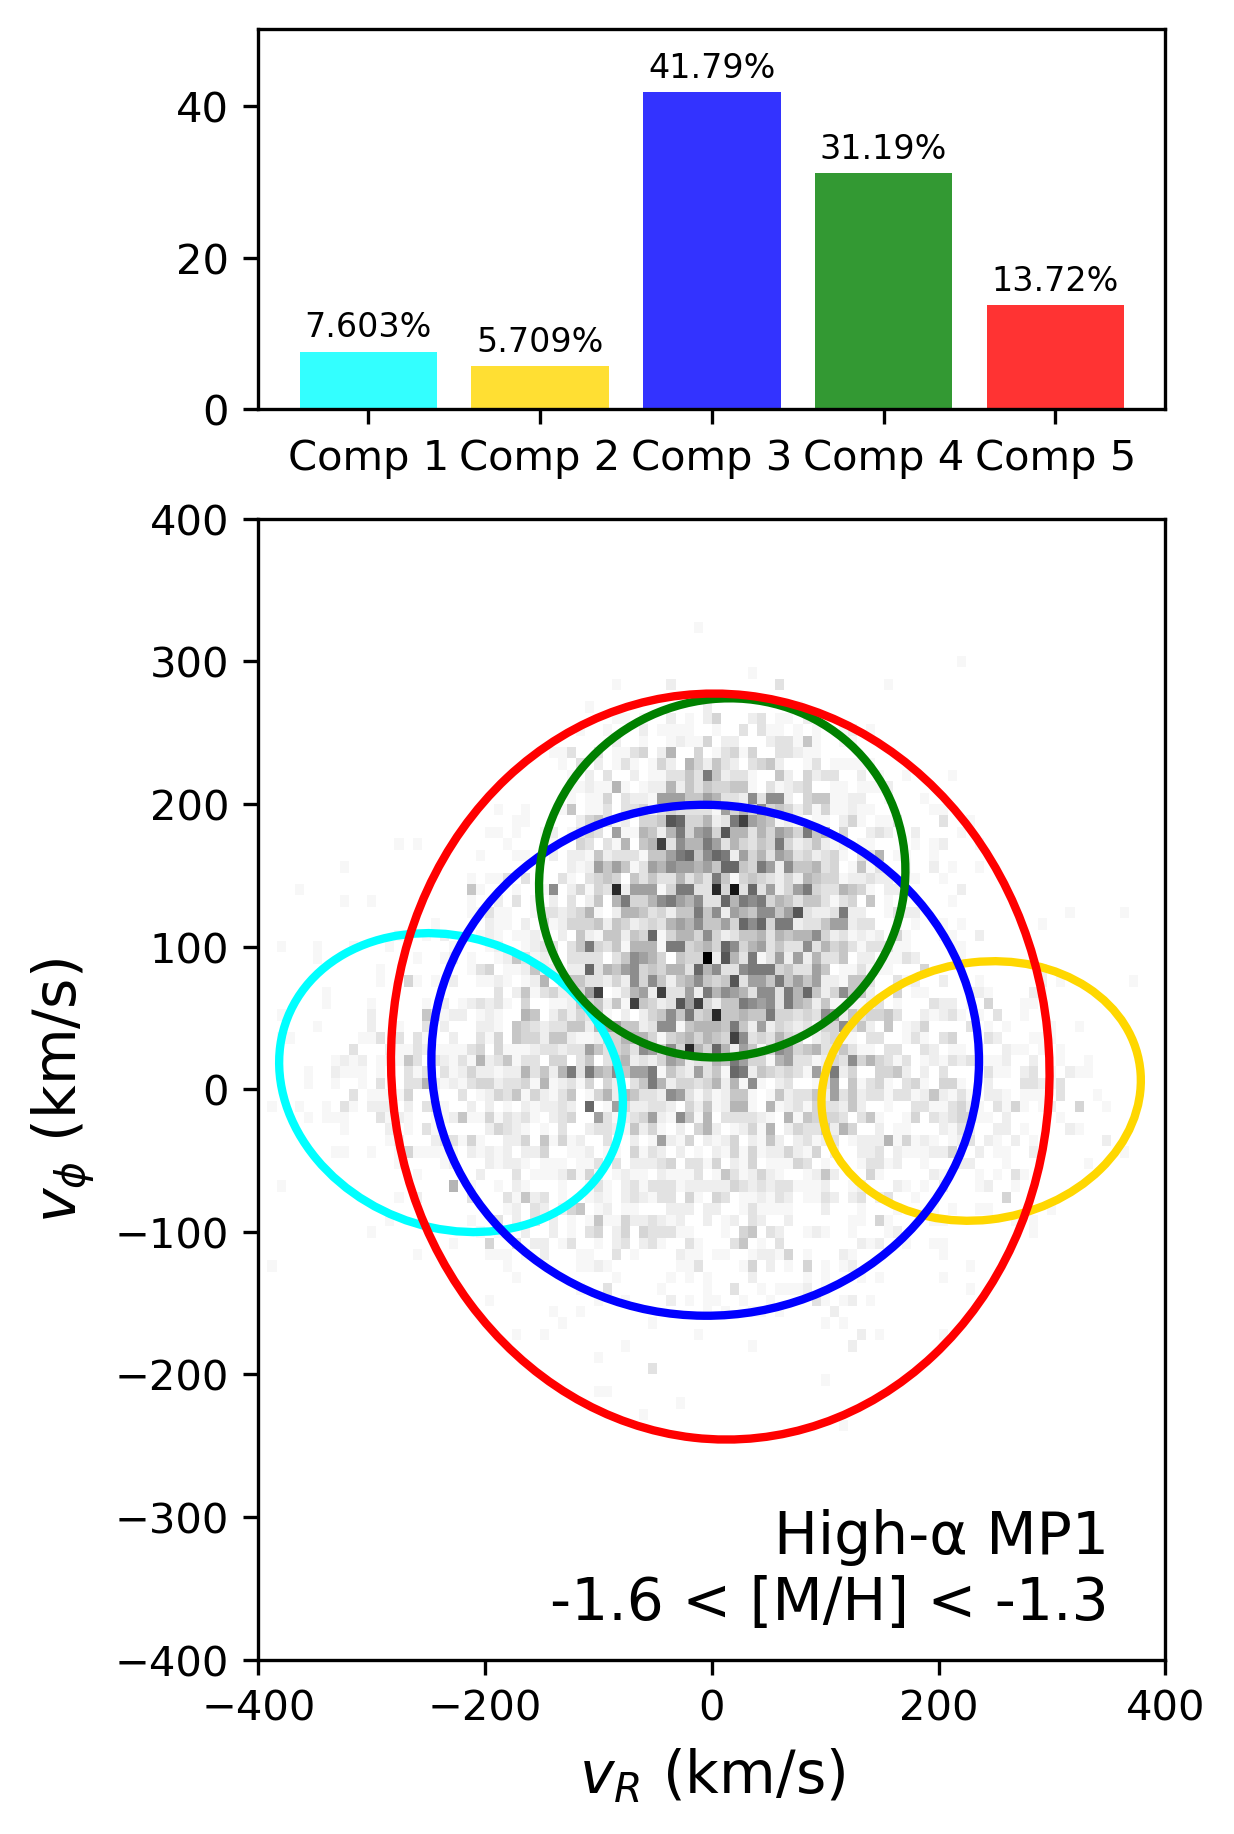
\includegraphics[width=\linewidth]{../figures/gmm_mp1_high_alpha_k5.png}
    \caption{MP1 ($k{=}4$)}
    \label{fig:mp1_hi}
  \end{subfigure}\hfill
  \begin{subfigure}{0.245\linewidth}
    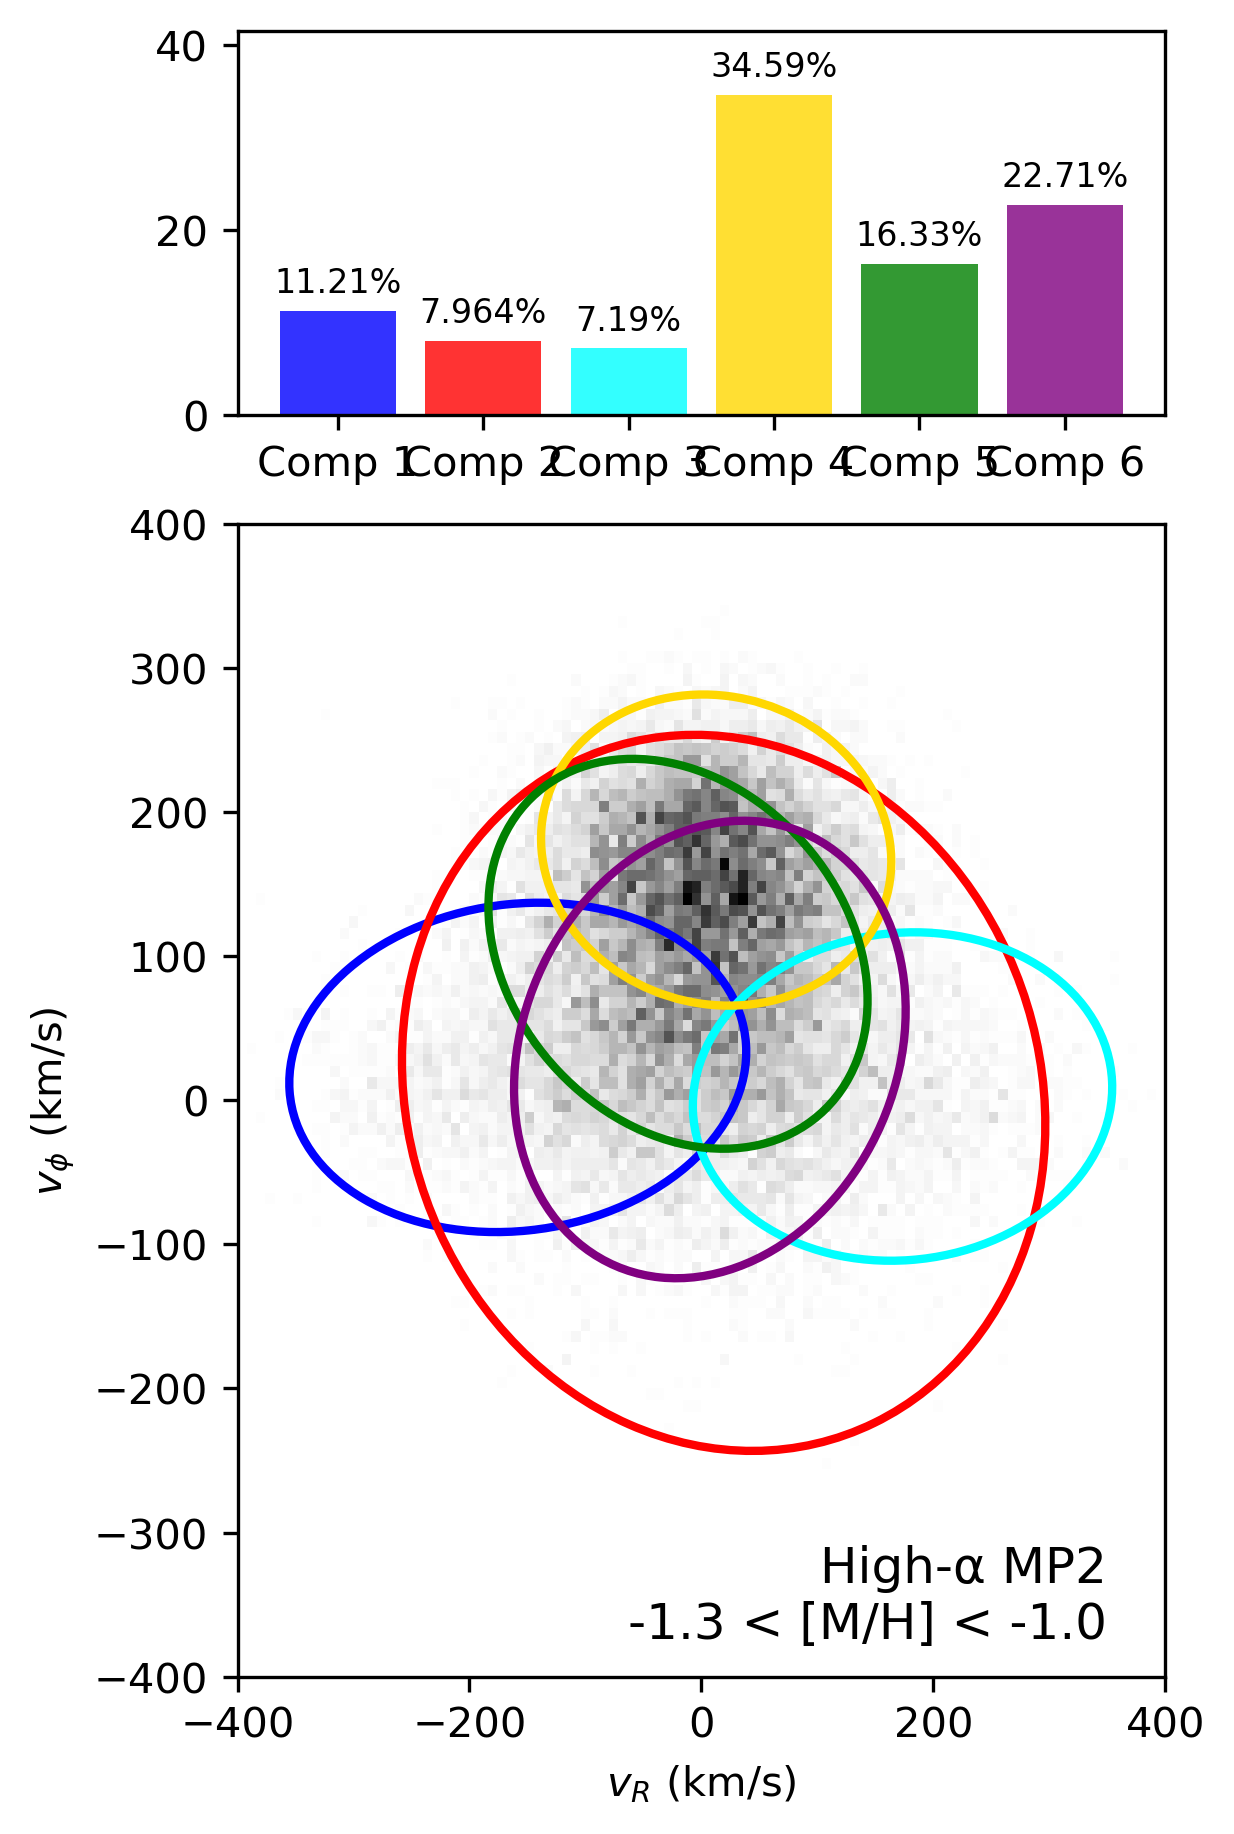
\includegraphics[width=\linewidth]{../figures/gmm_mp2_high_alpha_k6.png}
    \caption{MP2 ($k{=}6$)}
    \label{fig:mp2_hi}
  \end{subfigure}

  \caption{XD--GMM decomposition of high-$\alpha$ giants in four metallicity bins. Grey ellipses mark the $1\sigma$ contours of each Gaussian component.}
  \label{fig:gmm_4wide_hi}
\end{figure}

\begin{table}[H]
\centering
\begin{tabular}{lccccccc}
\hline
\textbf{Components} & \textbf{Weights (\%)} & $\mathbf{v_R}$ & $\boldsymbol{\sigma_R}$ & $\mathbf{v_\phi}$ & $\boldsymbol{\sigma_\phi}$ & $\mathbf{v_Z}$ & $\boldsymbol{\sigma_Z}$ \\
\hline
\multicolumn{8}{l}{\textbf{VMP:} $-3.0 < \mathrm{[M/H]} < -2.0$ (657 stars)} \\
Stationary halo     & 100.0 &   1.40 & 137.36 &  35.59 & 111.99 &  7.60 & 102.48 \\
\hline
\multicolumn{8}{l}{\textbf{IMP:} $-2.0 < \mathrm{[M/H]} < -1.6$ (5219 stars)} \\
Stationary halo     &  16.7 & -22.06 & 116.74 &  -8.55 & 135.74 & -2.64 & 125.40 \\
Prograde halo       &  51.9 &  10.84 &  90.56 &  84.51 &  94.79 & -0.76 &  69.42 \\
GS/E (1)            &  16.8 &-171.35 &  92.33 &  29.12 &  75.23 &  0.50 &  87.09 \\
GS/E (2)            &  14.5 & 180.48 &  91.48 &  -5.47 &  89.66 & -2.87 &  94.37 \\
\hline
\multicolumn{8}{l}{\textbf{MP1:} $-1.6 < \mathrm{[M/H]} < -1.3$ (10265 stars)} \\
Stationary halo     &   13.7 &   7.44 & 145.24 &  15.90 & 130.80 & -8.97 & 127.11 \\
Prograde halo       &   41.8 &  -5.85 & 120.77 &  20.31 &  89.59 & -1.29 &  72.85 \\
GS/E (1)            &   7.6 &-230.09 &  75.81 &   4.65 &  52.41 &  8.69 &  94.68 \\
GS/E (2)            &   5.7 & 237.61 &  70.43 &  -1.23 &  45.51 & -3.73 &  92.81 \\
Thick disc          &   31.2 &   9.18 &  80.79 & 148.23 &  62.97 &  2.99 &  68.92 \\
\hline
\multicolumn{8}{l}{\textbf{MP2:} $-1.3 < \mathrm{[M/H]} < -1.0$ (17314 stars)} \\
Stationary halo     &  17.7 &  15.91 & 141.96 &   2.13 & 101.75 & -1.68 &  98.90 \\
GS/E                &  30.5 & -18.50 & 141.08 &  22.42 &  56.55 & -2.40 &  77.98 \\
Thick Disk          &  51.8 &   5.22 &  76.27 & 159.54 &  57.94 & -0.83 &  67.18 \\
\hline
\end{tabular}
\caption{GMM component weights and kinematics for the high-$\alpha$ sequence.  
Velocities are in km\,s$^{-1}$. Weights indicate the fraction of stars per metallicity bin.}
\label{tab:gmm_higha_stats}
\end{table}


\subsection{Low alpha Gaussian Mixture Model Fit}

\begin{figure}[H]
  \centering
  \begin{subfigure}{0.24\linewidth}
    \centering
    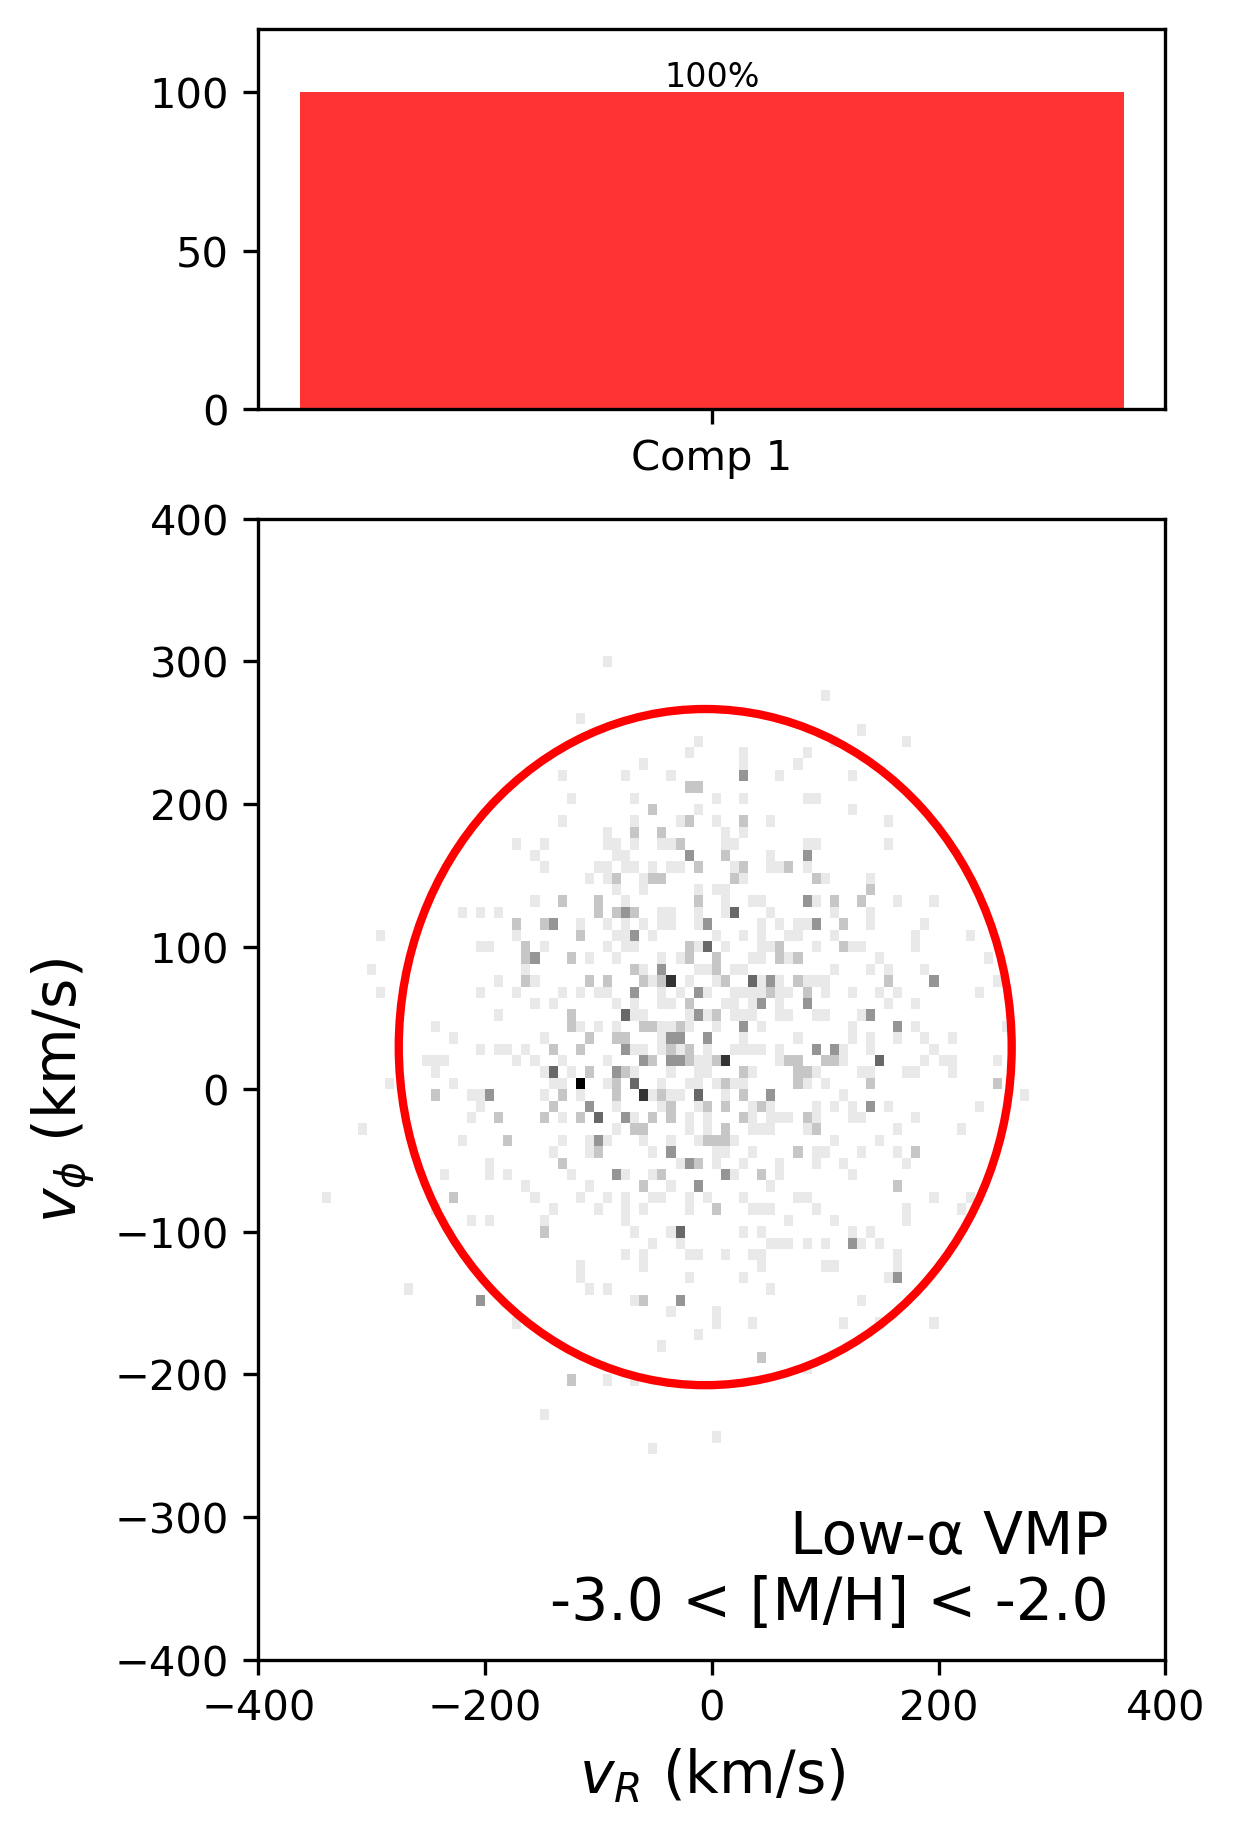
\includegraphics[width=\linewidth]{../figures/gmm_vmp_low_alpha_k1.png}
    \caption{VMP ($k{=}1$)}
    \label{fig:gmm_vmp_lo}
  \end{subfigure}\hfill
  \begin{subfigure}{0.24\linewidth}
    \centering
    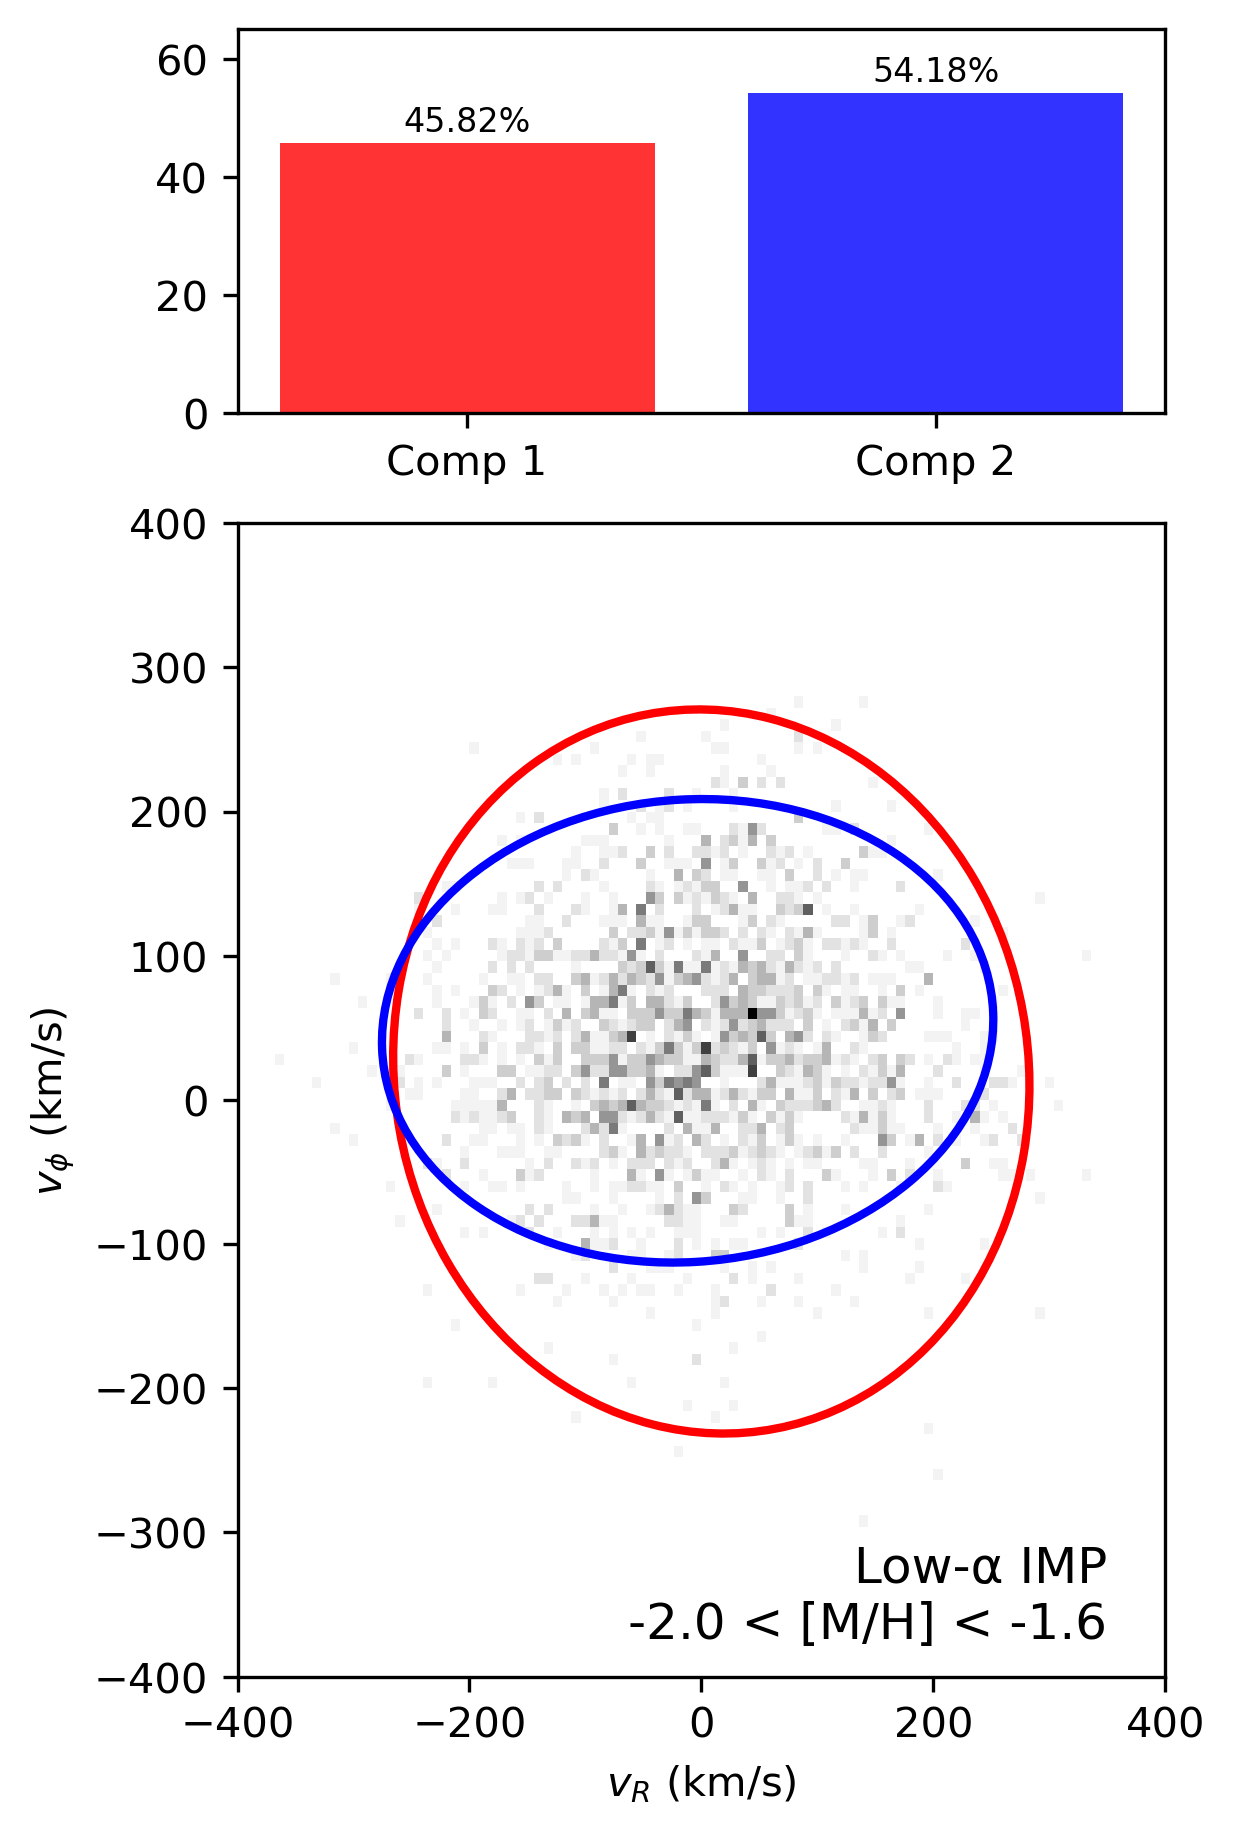
\includegraphics[width=\linewidth]{../figures/gmm_imp_low_alpha_k2.png}
    \caption{IMP ($k{=}2$)}
    \label{fig:gmm_imp_lo}
  \end{subfigure}\hfill
  \begin{subfigure}{0.24\linewidth}
    \centering
    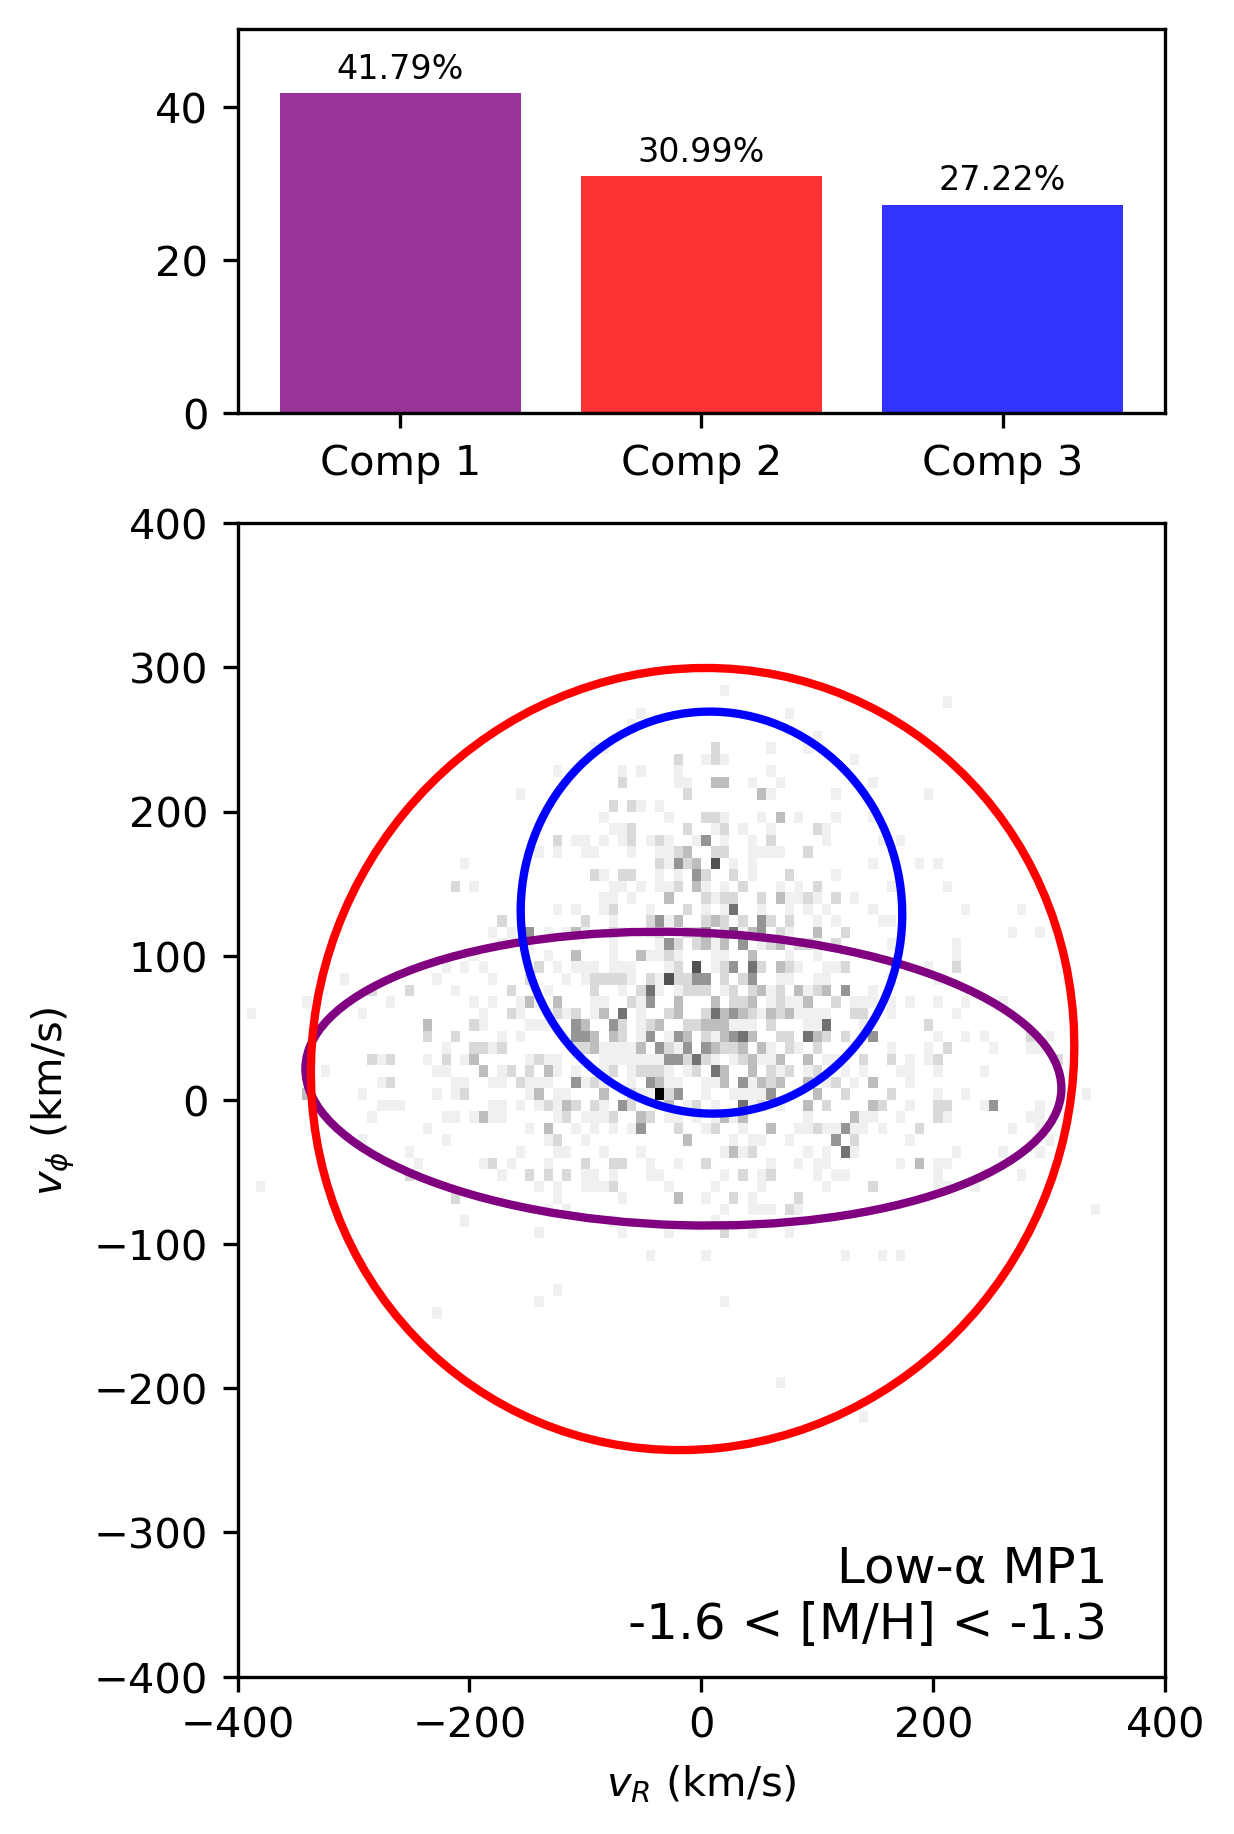
\includegraphics[width=\linewidth]{../figures/gmm_mp1_low_alpha_k4.png}
    \caption{MP1 ($k{=}4$)}
    \label{fig:gmm_mp1_lo}
  \end{subfigure}\hfill
  \begin{subfigure}{0.24\linewidth}
    \centering
    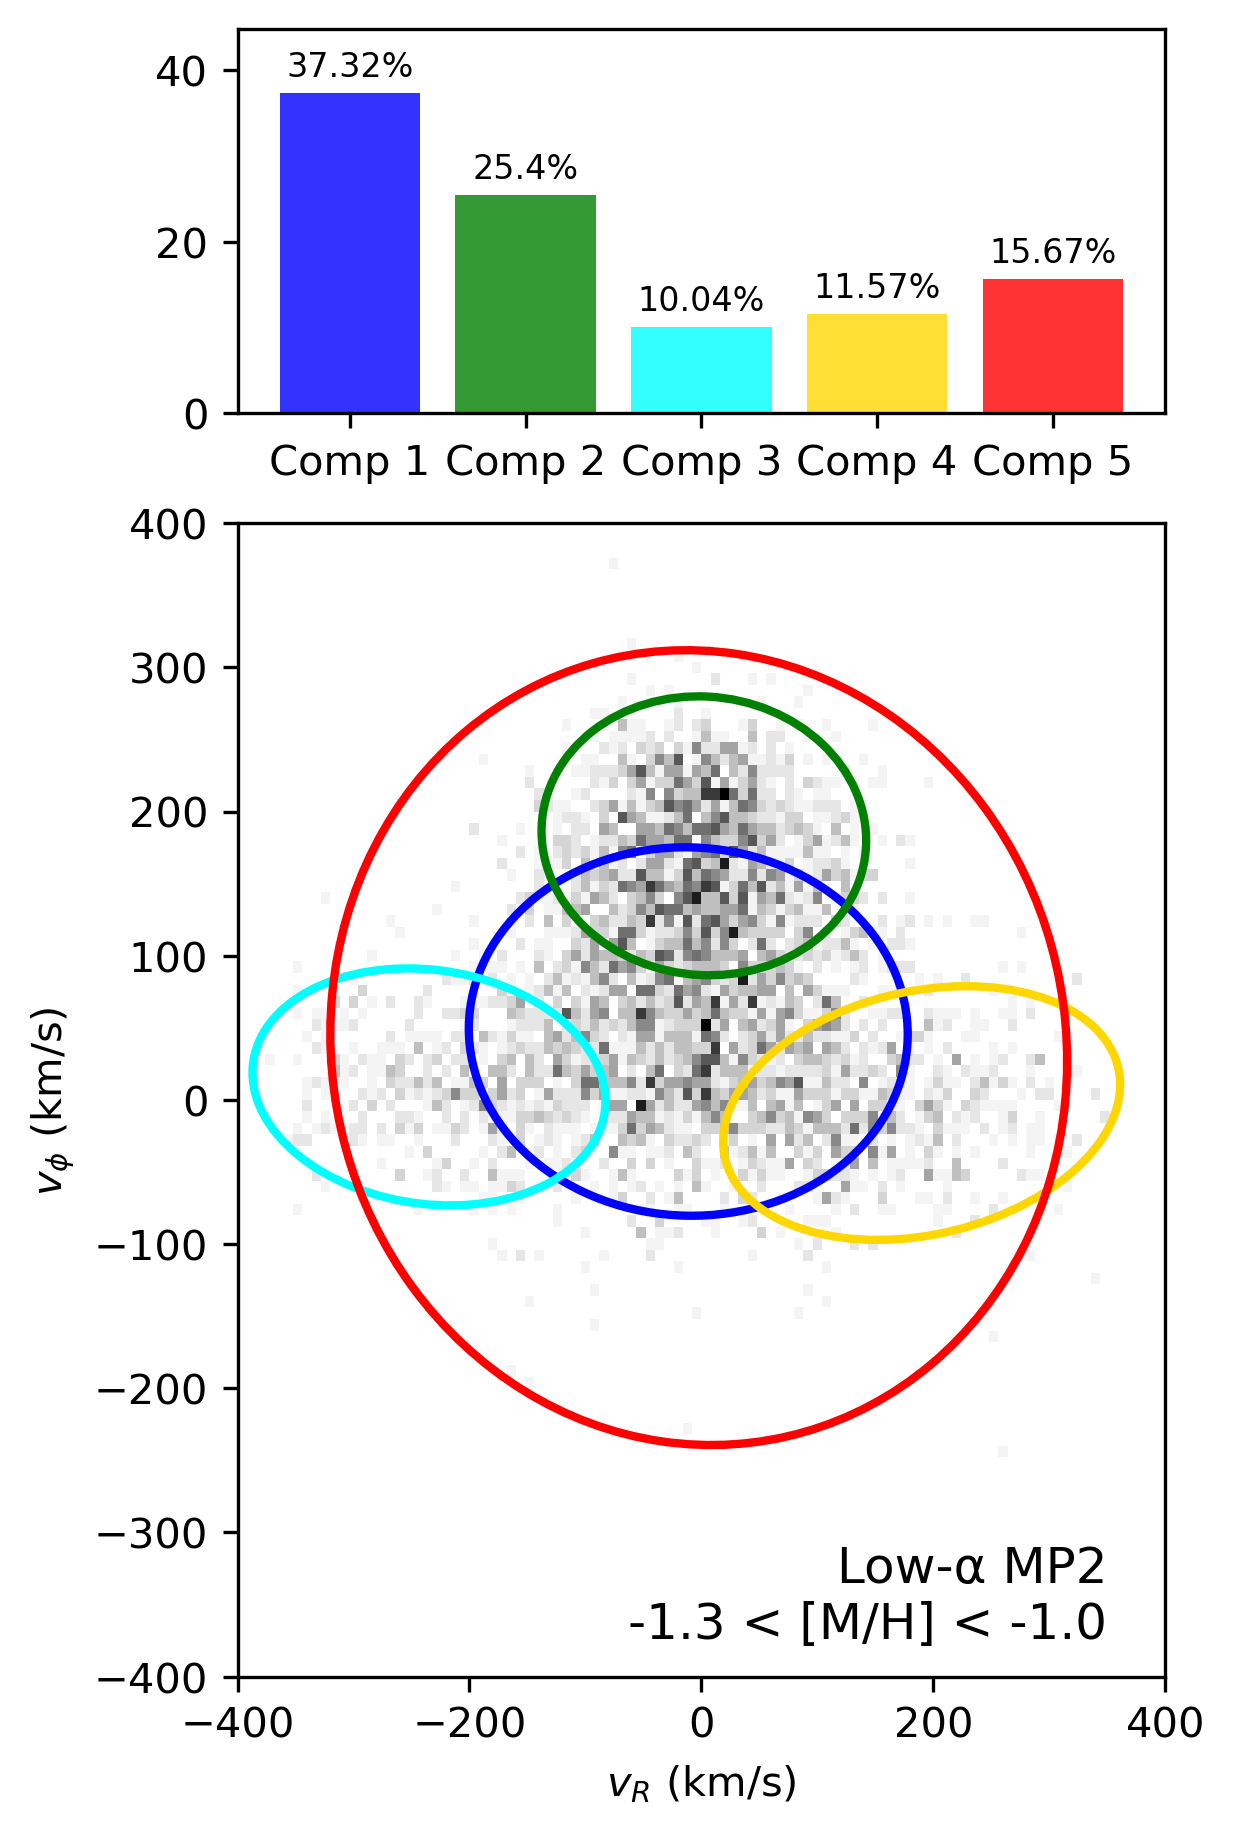
\includegraphics[width=\linewidth]{../figures/gmm_mp2_low_alpha_k6.png}
    \caption{MP2 ($k{=}6$)}
    \label{fig:gmm_mp2_lo}
  \end{subfigure}

  \caption{XD–GMM decomposition of low-$\alpha$ giants in four metallicity
           bins.  Grey ellipses show the $1\sigma$ contours of every Gaussian component.}
  \label{fig:gmm_lowalpha_panel}
\end{figure}

\begin{table}[H]
\centering
\begin{tabular}{lccccccc}
\hline
\textbf{Components} & \textbf{Weights (\%)} & $\mathbf{v_R}$ & $\boldsymbol{\sigma_R}$ & $\mathbf{v_\phi}$ & $\boldsymbol{\sigma_\phi}$ & $\mathbf{v_Z}$ & $\boldsymbol{\sigma_Z}$ \\
\hline
\multicolumn{8}{l}{\textbf{VMP:} $-3.0 < \mathrm{[M/H]} < -2.0$ (2929 stars)} \\
Stationary halo     & 100.0 &  -5.82 & 135.18 &  29.55 & 118.56 &  1.34 & 107.10 \\
\hline
\multicolumn{8}{l}{\textbf{IMP:} $-2.0 < \mathrm{[M/H]} < -1.6$ (3228 stars)} \\
Stationary halo     &  37.1 &  12.33 & 139.85 &  22.87 & 129.23 & -4.43 & 120.51 \\
Prograde halo       &  62.9 &  -7.34 & 138.11 &  49.68 &  91.25 &  4.08 &  75.99 \\
\hline
\multicolumn{8}{l}{\textbf{MP1:} $-1.6 < \mathrm{[M/H]} < -1.3$ (3603 stars)} \\
Stationary halo     &  31.0 &  -7.58 & 164.57 &  28.31 & 135.62 & -4.92 & 121.66 \\
GS/E                &  41.8 & -15.50 & 162.97 &  14.71 &  50.94 & -1.93 &  73.60 \\
Thick Disk          &  27.2 &   8.72 &  82.25 & 129.87 &  69.71 &  3.13 &  60.68 \\
\hline
\multicolumn{8}{l}{\textbf{MP2:} $-1.3 < \mathrm{[M/H]} < -1.0$ (7945 stars)} \\
Stationary halo     &  15.7 &  -2.30 & 158.84 &  36.24 & 137.81 &  2.81 & 131.10 \\
Prograde halo       &  37.3 & -11.31 &  94.62 &  47.39 &  63.89 & -1.18 &  63.12 \\
GS/E (1)            &  10.0 &-234.89 &  76.09 &   8.99 &  41.09 & 10.70 &  93.79 \\
GS/E (2)            &  11.6 & 189.95 &  85.58 &  -9.15 &  43.99 & -8.49 &  89.69 \\
Thick disc          &  25.4 &   2.13 &  69.98 & 183.15 &  48.36 &  1.75 &  54.21 \\
\hline
\end{tabular}
\caption{XD--GMM component weights and kinematics for the low-$\alpha$ sequence.  
         Velocities are in km\,s$^{-1}$. Weights are the fractional contribution of each component.}
\label{tab:gmm_lowa_stats}
\end{table}



%--------------------------------------------------
\subsection{Comparing the high and low \texorpdfstring{$\alpha$}{α} GMMs}
\label{subsec:gmm_comparison}

The two chemical sequences reveal markedly different kinematic evolutions.

\paragraph{Very–metal–poor regime (VMP\,: $[\mathrm{M/H}]<-2$).}
Both samples are modelled by a single, non–rotating halo Gaussian,
confirming the absence of disc‐like motions at the lowest abundances.
The velocity ellipsoids are nearly isotropic
($\sigma_{R}\!:\!\sigma_{\phi}\!:\!\sigma_{Z}\!\simeq\!1\!:\!1\!:\!1$),
but the high-$\alpha$ stars have a $\sim$10\,km\,s$^{-1}$ smaller
$\sigma_{\phi}$, hinting at an early imprint of prograde stirring.

\paragraph{Intermediate–metallicity regime (IMP\,: $-2.0<[\mathrm{M/H}]<-1.6$).}
Here the low-$\alpha$ population already splits into
stationary and prograde halo Gaussians of comparable
weight\,(46\%/54\%), whereas the high-$\alpha$ fit is
still dominated by four hot components, two of which trace the
Gaia–Sausage/Enceladus debris.  Thus rotation sets in
earlier for $\alpha$–poor stars, but remains dynamically hot.

\paragraph{Disc onset (MP1\,: $-1.6<[\mathrm{M/H}]<-1.3$).}
A thick-disc Gaussian appears in the high-$\alpha$ branch
(31\% weight, $v_\phi\!\sim\!140$\,km\,s$^{-1}$), while the
low-$\alpha$ mixture still requires five halo/GS/E components and shows no
cold disc type structure.  High-$\alpha$ stars therefore seem settle into a
rotation‐supported structure sooner.

\paragraph{Transition to disc dominance (MP2\,: $-1.3<[\mathrm{M/H}]<-1.0$).}
The high-$\alpha$ solution simplifies to three Gaussians: a thick disc
(49\%), a GS/E-like halo (34\%) and a small stationary
halo (17\%).  In contrast, the low-$\alpha$ fit remains
complex (six Gaussians) but now includes a thick disc
(26\%) alongside four halo/GS/E components. We expect an ultra-cold,
thin-disc Gaussian, however this is absent in this analysis due to sample selection choices.

 
From this analysis we infer that the high-$\alpha$ sequence evolves from a dispersion–supported 
halo to a kinematically warm thick disc between $[\mathrm{M/H}]\simeq-1.6$ and $-1.3$, whereas 
the low-$\alpha$ sequence starts to gain rotation at slightly lower metallicity yet remains 
halo–dominated until $[\mathrm{M/H}]\gtrsim-1.3$.  
The continuing prominence of GS/E–type Gaussians in every low-$\alpha$ bin highlights the dynamical 
footprint of the last major merger on these stars, while the simpler three–component 
mix in the high-$\alpha$/MP2 slice suggests an earlier, cleaner consolidation of the \textit{in-situ} thick disc.  
Taken together, the two sequences trace the “two-phase’’ disc‐building picture of \citet{Haywood2013}: 
an early, $\alpha$-rich epoch that settles into the thick disc, followed by a later, 
$\alpha$-poor phase that assembles the thin disc from progressively 
enriched and dynamically cooler gas.



%------------------------------------------------------------------
\section{Discussion} \label{sec:discussion}
%------------------------------------------------------------------







\section{problems with \citet{zhang2024existencemetalpoordiscmilky}}

i do not believe random initial coditions are used for bic and gmm fitting
in order to get results with astrophsyical meaning, k means inistialisation is required
this is because gmms are very senstitive to initial conditions, and can easily get stuck in local minima.

\section{Extension direction}

\section{Conclusion}



\newpage
\bibliographystyle{abbrvnat}
\bibliography{references}




\end{document}
